\documentclass[titlepage]{article}

\usepackage[letterpaper,margin=1in,footskip=0.25in]{geometry}
\usepackage[hidelinks]{hyperref}
\usepackage{fancyhdr}
\usepackage{csquotes}
\usepackage{amsmath}
\usepackage{tikz}
\usepackage{subcaption}
\usepackage{graphicx}
\usepackage{amssymb}
\usepackage{float}

\MakeOuterQuote{"}

\numberwithin{figure}{section}
\numberwithin{table}{section}
\numberwithin{equation}{section}

\usetikzlibrary{knots,decorations.markings,positioning}
\tikzset{mini/.style={scale=0.15,baseline={(0,-0.09)},every path/.style={knot=red,thick}}}

\newcommand{\dq}[2]{``#1" (#2).}
\newcommand{\lbq}{<\hspace{-3pt}}
\newcommand{\rbq}{\hspace{-3pt}>}
\newcommand{\bpunknot}{\tikz[mini]{
    \draw circle (1cm);
}}
\newcommand{\vertopen}{\tikz[mini,every to/.style={bend angle=45,looseness=1.3}]{
    \draw (-1,1) to[bend left] (-1,-1);
    \draw (1,1) to[bend right] (1,-1);
}}
\newcommand{\horiopen}{\tikz[mini,every to/.style={bend angle=45,looseness=1.3}]{
    \draw (-1,-1) to[bend left] (1,-1);
    \draw (-1,1) to[bend right] (1,1);
}}

\renewcommand{\labelitemiii}{\scriptsize$\blacksquare$}

\title{{\Huge\emph{The Knot Book}}\\[5pt]\textcolor{gray!60!black}{Notes}\vspace{-0.5em}}
\author{Steven Labalme}
\date{\today}

\begin{document}




\pagenumbering{gobble}
\maketitle



\pagenumbering{roman}
\tableofcontents
\listoffigures
\listoftables
\newpage



\pagenumbering{arabic}
\pagestyle{fancy}
\fancyhf{}
\rfoot{Labalme \thepage}
\renewcommand{\headrulewidth}{0pt}
\section{Introduction}\label{sse:intro}
\subsection{Introduction}\label{sss:Introduction}
\begin{itemize}
    \item \textbf{Knot}: \dq{A knotted loop of string, except that we think of the string as having no thickness, its cross-section being a single point}{2}
    \item Do not distinguish between a `nice, even' knot and one that has been deformed through space.
    \item \textbf{Unknot}: \dq{The simplest knot of all\dots the unknoted circle}{2} \emph{Also known as} \textbf{trivial knot}. See Figure \ref{fig:circletrefoila}.
    \item \textbf{Trefoil knot}: \dq{The next simplest knot}{2} See Figure \ref{fig:circletrefoilb}.
    \begin{figure}[h!]
        \centering
        \begin{subfigure}{0.2\linewidth}
            \centering
            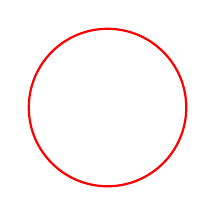
\begin{tikzpicture}
                \draw[red,thick] (0,0) circle (1cm);
            \end{tikzpicture}
            \caption{Trivial knot.}
            \label{fig:circletrefoila}
        \end{subfigure}
        \begin{subfigure}{0.2\linewidth}
            \centering
            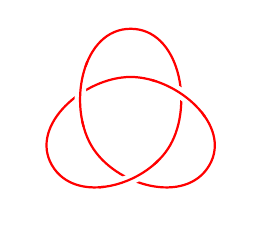
\begin{tikzpicture}
                \begin{knot}[
                    consider self intersections,
                    clip width=5
                ]
                    % could be defined with a combination of polar coordinates and foreach...
                    \strand[red,thick] (1,{3^0.5})
                        to [out=0,in=60] (1.5,0.25)
                        to [out=240,in=-60] (0,0)
                        to [out=120,in=180] (1,1.12)
                        to [out=0,in=60] (2,0)
                        to [out=240,in=-60] (0.5,0.25)
                        to [out=120,in=180] cycle
                    ;
                    \flipcrossings{1,3}
                \end{knot}
            \end{tikzpicture}
            \caption{Trefoil knot.}
            \label{fig:circletrefoilb}
        \end{subfigure}
        \caption{Projections of the two simplest knots.}
        \label{fig:circletrefoil}
    \end{figure}
    \item \textbf{Projection}: A picture of a knot, such as those in Figure \ref{fig:circletrefoil}.
    \begin{itemize}
        \item The same knots can have multiple projections (as they are deformed in space).
    \end{itemize}
    \item \textbf{Crossings}: The places in a projection where a knot crosses itself.
    \begin{itemize}
        \item The trefoil knot in Figure \ref{fig:circletrefoilb} is a \underline{three-crossing knot} because it crosses itself 3 times.
        \item Any one-crossing knot is trivial.
        \item \emph{Exercise 1.2}: Any two-crossing knot must be trivial because the simplest nontrivial knot is the trefoil knot, which has three crossings.
    \end{itemize}
    \item Atoms were originally thought to be tangles (knots) in the ether of the universe, but when chemists moved on, mathematicians took up knot theory. In the 1980s, biochemists began to see applications of knot theory in their research (see Section \ref{sse:biochemphys}).
    \item \textbf{Topology}: \dq{The study of the properties of geometric objects that are preserved under deformations}{6}
    \begin{itemize}
        \item Knot theory is a subfield of topology (see Section \ref{sse:topology}).
    \end{itemize}
    \begin{figure}[h!]
        \centering
        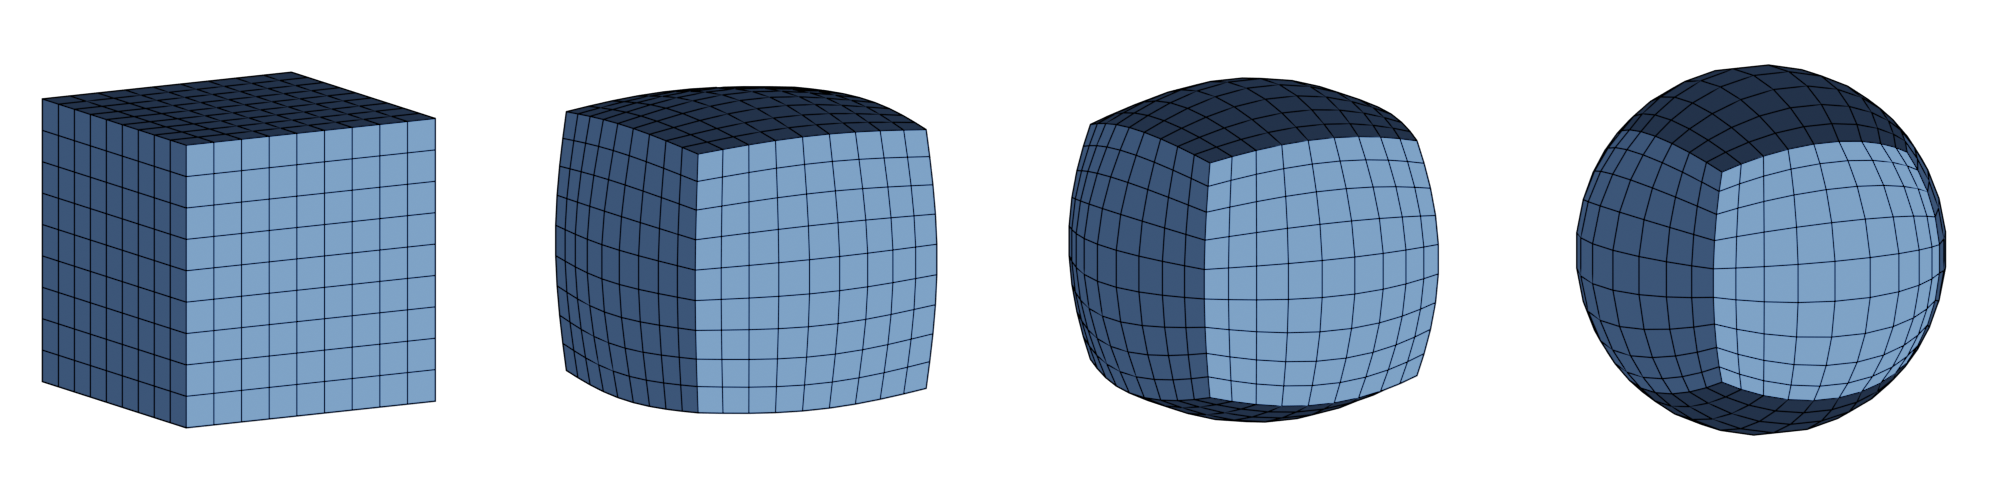
\includegraphics[width=0.7\linewidth]{Blender/CubeSphere.png}
        \caption{Deformation of a cube into a sphere.}
        \label{fig:cubesphere}
    \end{figure}
    \item Any knot can have a projection with as many crossings as desired.
    \item \textbf{Alternating knot}: \dq{A knot with a projection that has crossings that alternate between over and under as one travels around the knot in a fixed direction}{7}
    \begin{itemize}
        \item The trefoil is such a knot.
    \end{itemize}
    \item \emph{Exercise 1.7*}: By changing some of the crossings from over to under or vice versa, any projection of a knot can be made into a projection of the unknot$^[$\footnote{How can I \emph{show} something? How can I do these proofs? What kind of logic solves one of these? See Section \ref{sss:UnknottingNumber} for a direct proof of/solution to \emph{Exercise 1.7}.}$^]$. See Figure \ref{fig:knottotrivial}.
    \begin{figure}[h!]
        \centering
        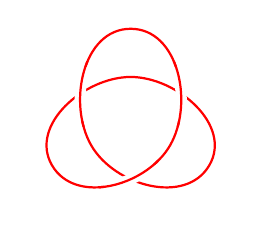
\begin{tikzpicture}
            \begin{knot}[
                consider self intersections,
                clip width=5
            ]
                \strand[red,thick] (1,{3^0.5})
                    to [out=0,in=60] (1.5,0.25)
                    to [out=240,in=-60] (0,0)
                    to [out=120,in=180] (1,1.12)
                    to [out=0,in=60] (2,0)
                    to [out=240,in=-60] (0.5,0.25)
                    to [out=120,in=180] cycle
                ;
                \flipcrossings{3}
            \end{knot}
        \end{tikzpicture}
        \caption{A projection of the unknot evoking the trefoil knot.}
        \label{fig:knottotrivial}
    \end{figure}
\end{itemize}


\subsection{Composition of Knots}\label{sss:Composition}
\begin{itemize}
    \item \textbf{Composition} (of two knots): \dq{A new knot obtained by removing a small arc from two knot projections and then connecting the four endpoints by two new arcs}{7}
    \begin{itemize}
        \item If two knots are designated $J$ and $K$, then their composition is denoted $J\#K$.
        \item Do not overlap the projections and choose two arcs that are on the outside to avoid new crossings.
        \item Make sure that the new arcs do not cross any of the the original knot projections or each other.
    \end{itemize}
    \item \textbf{Composite knot}: A knot that \dq{can be expressed as the composition of two knots, neither of which is the trivial knot}{8}
    \begin{itemize}
        \item This definition is analogous to composite integers, where an integer is \underline{composite} if it is the product of positive integers, neither of which is $1$.
        \item Similarly, if we compose any knot with the unknot, we get the same knot back.
    \end{itemize}
    \item \textbf{Factor knots}: \dq{The knots that make up the composite knot}{8}
    \item \textbf{Prime knot}: \dq{A knot [that] is not the composition of any two nontrivial knots}{9}
    \item The unknot, trefoil knot, and figure-eight knots are all prime (see Section \ref{sss:GenusSeifert}).
    \begin{itemize}
        \item The unknot is not composite for the same reason that 1 is not the product of two integers greater than 1.
    \end{itemize}
    \begin{figure}[h!]
        \centering
        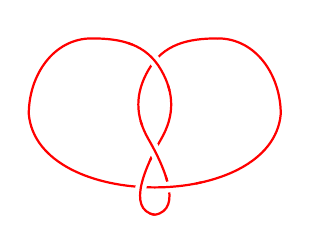
\begin{tikzpicture}[scale=0.8]
            \begin{knot}[
                clip width=5
            ]
                % Use looseness=# key to stretch out lengths!
                \strand[red,thick]       (0,0)
                    to [out=-85,in=-95]  (4,0)
                    to [out=90,in=0]     (3,1.2)
                ;
                \strand[red,thick]       (3,1.2)
                    to [out=180,in=60]   (1.9,0.7)
                    to [out=-120,in=120] (1.9,-0.4)
                    to [out=-60,in=10]   (2,-1.6)
                ;
                \strand[red,thick]       (2,-1.6)
                    to [out=170,in=-120] (2.1,-0.4)
                    to [out=60,in=-60]   (2.1,0.7)
                    to [out=120,in=0]    (1,1.2)
                    to [out=180,in=90]   (0,0)
                ;
                \flipcrossings{2,3}
            \end{knot}
        \end{tikzpicture}
        \caption{The figure-eight knot.}
        \label{fig:figure8knot}
    \end{figure}
    \item Similar to integers, \dq{a composite knot factors into a unique set of prime knots}{10}
    \item \emph{Exercise 1.8}: Using the appendix table, identify the factor knots that make up the composite knot in Figure \ref{fig:compos1}.
    \begin{itemize}
        \item The knot in Figure \ref{fig:compos1} is the composition of two projections of $5_2$.
    \end{itemize}
    \newpage
    \begin{figure}[h!]
        \centering
        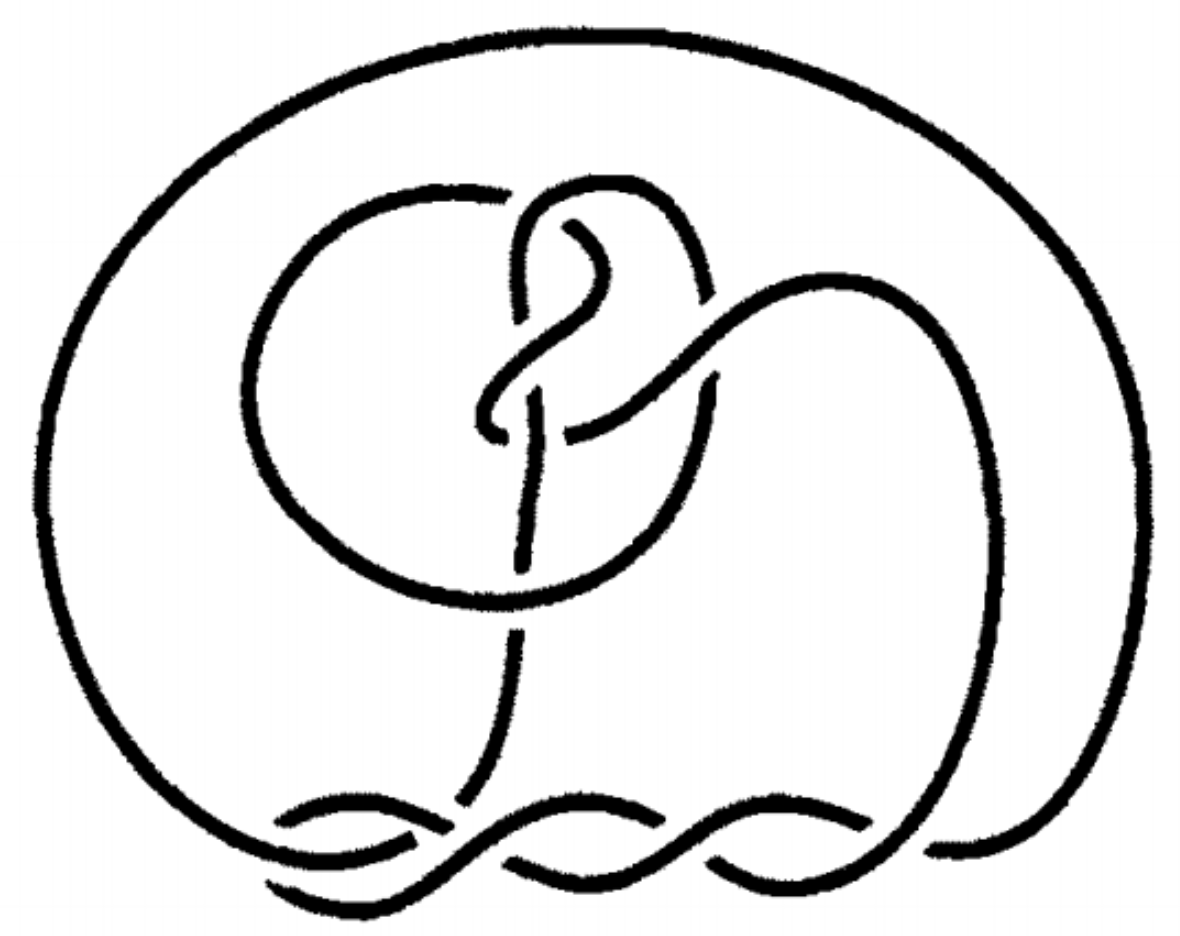
\includegraphics[width=0.2\linewidth]{Blender/compos1.png}
        \caption{The composite knot.}
        \label{fig:compos1}
    \end{figure}
    \item \emph{Exercise 1.9}: Show that the knot in Figure \ref{fig:compos2a} is composite.
    \begin{figure}[h!]
        \centering
        \begin{subfigure}[b]{0.3\textwidth}
            \centering
            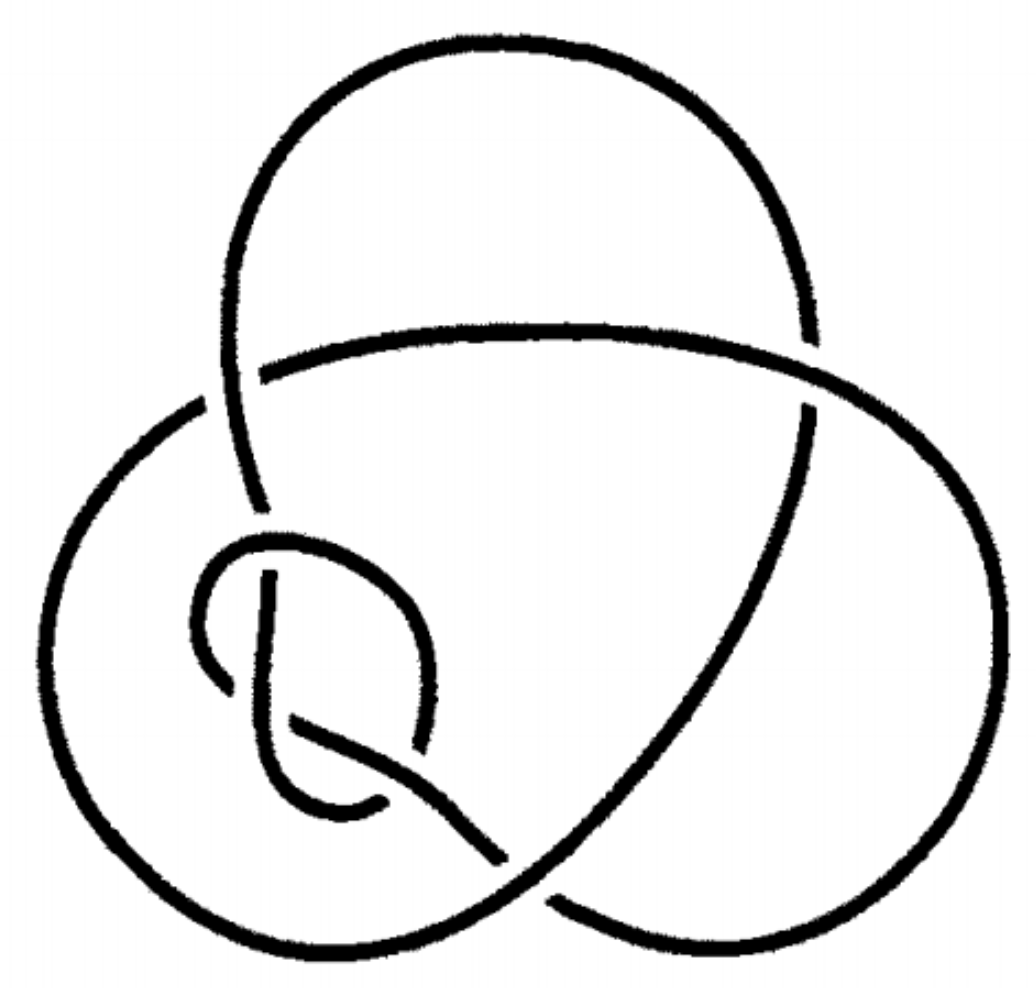
\includegraphics[width=0.5\textwidth]{Blender/compos2.png}
            \caption{The composite knot.}
            \label{fig:compos2a}
        \end{subfigure}
        \begin{subfigure}[b]{0.3\textwidth}
            \centering
            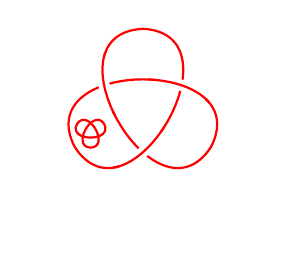
\begin{tikzpicture}
                \begin{knot}[
                    clip width=5,
                    consider self intersections
                ]
                    % Why don't polar coordinates mesh with figures?
                    \strand[red,thick] (90:1)
                        \foreach \x in {1,2,3} {
                            to [bend left=117,looseness=1.9] ({90+120*\x}:1)
                        }
                    ;
                    \flipcrossings{1,3}
                \end{knot}
                \begin{knot}[
                    clip width=5,
                    consider self intersections,
                    rotate=60,
                    scale=0.2,
                    xshift=-3cm,yshift=2.1cm
                ]
                    \strand[red,thick] (90:1)
                        \foreach \x in {1,2,3} {
                            to [bend left=117,looseness=1.9] ({90+120*\x}:1)
                        }
                    ;
                    \flipcrossings{1,3}
                \end{knot}
            \end{tikzpicture}
            \vspace{-0.8cm}
            \caption{Factors.}
            \label{fig:compos2b}
        \end{subfigure}
        \caption{Factorization of a `double trefoil.'}
        \label{fig:compos2}
    \end{figure}
    \item There is more than one way to take the composition of two knots (by removing different arcs).
    \begin{itemize}
        \item This is not analogous to multiplication --- a break in the pattern.
    \end{itemize}
    \item \textbf{Orientation}: A direction to travel around the knot. Denoted by placing \dq{coherently directed arrows along the projection of the knot in the direction of our choice}{10} A knot with such arrows is \textbf{oriented}.
    \begin{itemize}
        \item All compositions $J\#K$ where the orientations of $J$ and $K$ \underline{do} match up will yield the same composite knot.
        \begin{itemize}
            \item $J$ can be `slid around' $J\#K$ until it reaches the second position where the composition was taken.
        \end{itemize}
        \item All compositions $J\#K$ where the orientations of $J$ and $K$ \underline{do not} match up will yield the same composite knot.
        \item These two compositions can be distinct.
    \end{itemize}
    \begin{figure}[h!]
        \centering
        \begin{tikzpicture}
            \begin{knot}[
                clip width=5,
                consider self intersections
            ]
                \strand[red,thick,
                decoration={markings,
                mark=at position 0.2 with {\arrow{>}}},
                postaction={decorate}] (90:1)
                    \foreach \x in {1,2,3} {
                        to [bend left=117,looseness=1.9] ({90+120*\x}:1)
                    }
                ;
                \flipcrossings{1,3}
            \end{knot}
        \end{tikzpicture}
        \vspace{-0.8cm}
        \caption{Orientation notation.}
        \label{fig:orientnotation}
    \end{figure}
    \item \textbf{Invertible}: A knot that can be deformed back to itself so that an orientation on it is sent to the opposite orientation.
    \begin{itemize}
        \item \dq{In the case that one of the two knots is invertible, say $J$, we can always deform the composite knot so that the orientation on $K$ is reversed, and hence so that the orientations of $J$ and $K$ always match. Therefore, there is only one composite knot that we can construct from the two knots}{11}
    \end{itemize}
    \item To determine the possible compositions of knots, it is necessary to know which knots are invertible, but no general technique has yet been discovered.
\end{itemize}


\subsection{Reidemeister Moves}
\begin{itemize}
    \item \textbf{Ambient isotropy}: \dq{The movement of the string through three-dimensional space without letting it pass through itself}{12}
    \item \textbf{Planar isotropy}: A deformation of \dq{the projection plane as if it were made of ruber with the projection drawn upon it}{12}
    \begin{itemize}
        \item Stretching, squeezing, rotating, bending single arcs, etc.
    \end{itemize}
    \item \textbf{Reidemeister move}: \dq{One of three ways to change a projection of the knot that \emph{will} change the relation between the crossings}{13}
    \item \textbf{First Reidemeister move}: \dq{Put in or take out a twist in the knot}{13} See Figure \ref{fig:reidema}. \emph{Also known as} \textbf{type I Reidemeister move}.
    \item \textbf{Second Reidemeister move}: \dq{Either add two crossings or remove two crossings}{13} See Figure \ref{fig:reidemb}. \emph{Also known as} \textbf{type II Reidemeister move}.
    \item \textbf{Third Reidemeister move}: \dq{Slide a strand of the knot from one side of a crossing to the other side of the crossing}{13} See Figure \ref{fig:reidemc}. \emph{Also known as} \textbf{type III Reidemeister move}.
    \begin{itemize}
        \item Note that the crossings in Figure \ref{fig:reidem} can be reversed and the move will still be classified under the same category.
    \end{itemize}
    \begin{figure}[h!]
        \centering
        \begin{subfigure}[b]{0.3\linewidth}
            \centering
            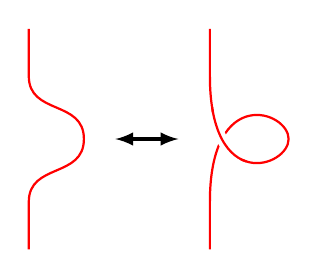
\begin{tikzpicture}
                \draw[red,thick,xshift=-1.5cm] (0,0.4) -- (0,1) .. controls (0,1.5) and (0.7,1.3) .. (0.7,1.8) .. controls (0.7,2.3) and (0,2.1) .. (0,2.6) -- (0,3.2);
                \draw[very thick,latex-latex] (-0.4,1.8) -- (0.4,1.8);
                \begin{knot}[
                    xshift=0.8cm,
                    consider self intersections=no splits,
                    clip width=5,
                    flip crossing=1
                ]
                    \strand[red,thick] (0,0.4) -- (0,1) to [out=90,in=90,out looseness=3,in looseness=0.7] (1,1.8) to [out=-90,in=-90,in looseness=3,out looseness=0.7] (0,2.6) -- (0,3.2);
                \end{knot}
            \end{tikzpicture}
            \caption{Type I Reidemeister move.}
            \label{fig:reidema}
        \end{subfigure}
        \begin{subfigure}[b]{0.3\linewidth}
            \centering
            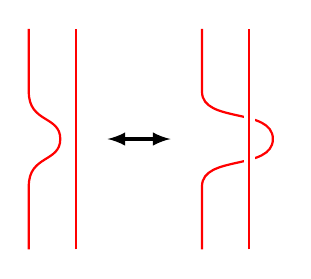
\begin{tikzpicture}
                \draw[red,thick,xshift=-1.4cm] (0,0.4) -- (0,1.2) .. controls (0,1.6) and (0.4,1.5) .. (0.4,1.8) .. controls (0.4,2.1) and (0,2) .. (0,2.4) -- (0,3.2);
                \draw[red,thick,xshift=-1.4cm] (0.6,0.4) -- (0.6,3.2);
                \draw[very thick,latex-latex] (-0.4,1.8) -- (0.4,1.8);
                \begin{knot}[
                    xshift=0.8cm,
                    clip width=5
                ]
                    \strand[red,thick] (0,0.4) -- (0,1.2) .. controls (0,1.6) and (0.9,1.4) .. (0.9,1.8) .. controls (0.9,2.2) and (0,2) .. (0,2.4) -- (0,3.2);
                    \strand[red,thick] (0.6,0.4) -- (0.6,3.2);
                    \flipcrossings{1,2}
                \end{knot}
            \end{tikzpicture}
            \caption{Type II Reidemeister move.}
            \label{fig:reidemb}
        \end{subfigure}\\
        \vspace{1em}
        \begin{subfigure}[b]{0.6\linewidth}
            \centering
            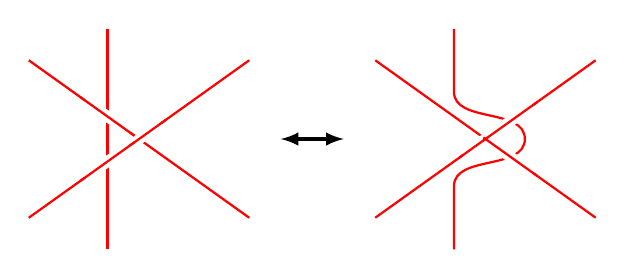
\begin{tikzpicture}
                \begin{knot}[
                    xshift=-2.2cm,
                    clip width=5
                ]
                    \strand[red,thick] (-1.4,0.8) -- (1.4,2.8);
                    \strand[red,thick] (-1.4,2.8) -- (1.4,0.8);
                    \strand[red,thick] (-0.4,0.4) -- (-0.4,3.2);
                \end{knot}
                \draw[very thick,latex-latex] (-0.4,1.8) -- (0.4,1.8);
                \begin{knot}[
                    xshift=2.2cm,
                    clip width=5
                ]
                    \strand[red,thick] (-1.4,0.8) -- (1.4,2.8);
                    \strand[red,thick] (-1.4,2.8) -- (1.4,0.8);
                    \strand[red,thick] (-0.4,0.4) -- (-0.4,1.2) .. controls (-0.4,1.6) and (0.5,1.4) .. (0.5,1.8) .. controls (0.5,2.2) and (-0.4,2) .. (-0.4,2.4) -- (-0.4,3.2);
                \end{knot}
            \end{tikzpicture}
            \caption{Type III Reidemeister move.}
            \label{fig:reidemc}
        \end{subfigure}
        \caption{Reidemeister moves.}
        \label{fig:reidem}
    \end{figure}
    \item All Reidemeister moves are ambient isotropies.
    \item \dq{If we have two distinct projections of the same knot, we can get from the one projection to the other by a series of Reidemeister moves and planar isotropies}{14}
    \item \textbf{Amphicheiral}: A knot that \dq{is equivalent to its mirror image, that is, the knot obtained by changing every crossing\dots to the opposite crossing}{14-15} \emph{Also known as} \textbf{achiral} \emph{by chemists.}
    \begin{itemize}
        \item A knot and its mirror image are distinct unless the knot is amphicheiral.
        \item See Section \ref{sse:biochemphys} for more on amphicheirality.
    \end{itemize}
    \newpage
    \item \emph{Exercise 1.10}: Show that the two projections in Figure \ref{fig:ex1-10} represent the same knot by finding a series of Reidemeister moves from one to the other.
    \begin{figure}[h!]
        \centering
        \begin{subfigure}[b]{0.2\linewidth}
            \centering
            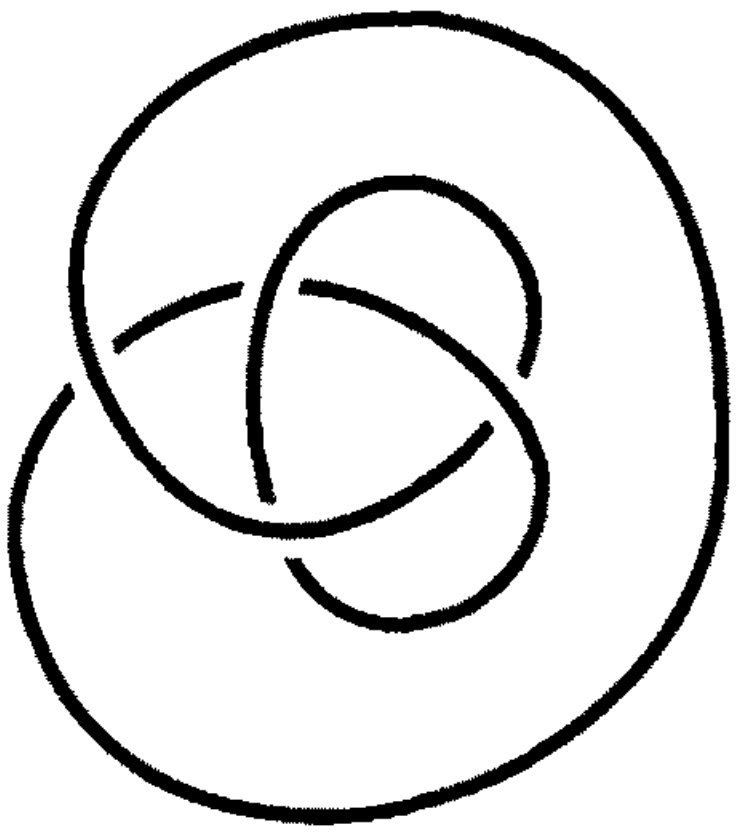
\includegraphics[width=0.6\linewidth]{Blender/ex1-10a.png}
            \caption{Initial projection.}
            \label{fig:ex1-10a}
        \end{subfigure}
        \begin{subfigure}[b]{0.2\linewidth}
            \centering
            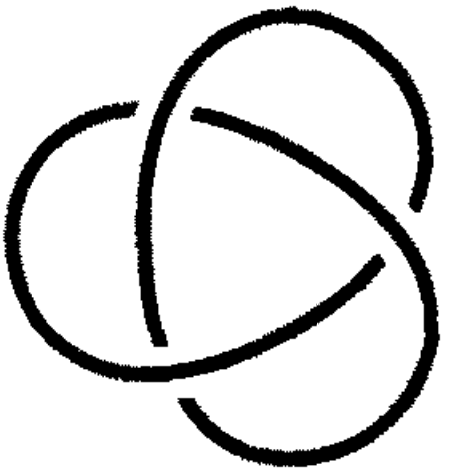
\includegraphics[width=0.4\linewidth]{Blender/ex1-10b.png}
            \vspace{4mm}
            \caption{Final projection.}
            \label{fig:ex1-10b}
        \end{subfigure}
        \caption{Finding Reidemeister moves.}
        \label{fig:ex1-10}
    \end{figure}
    \begin{figure}[h!]
        \centering
        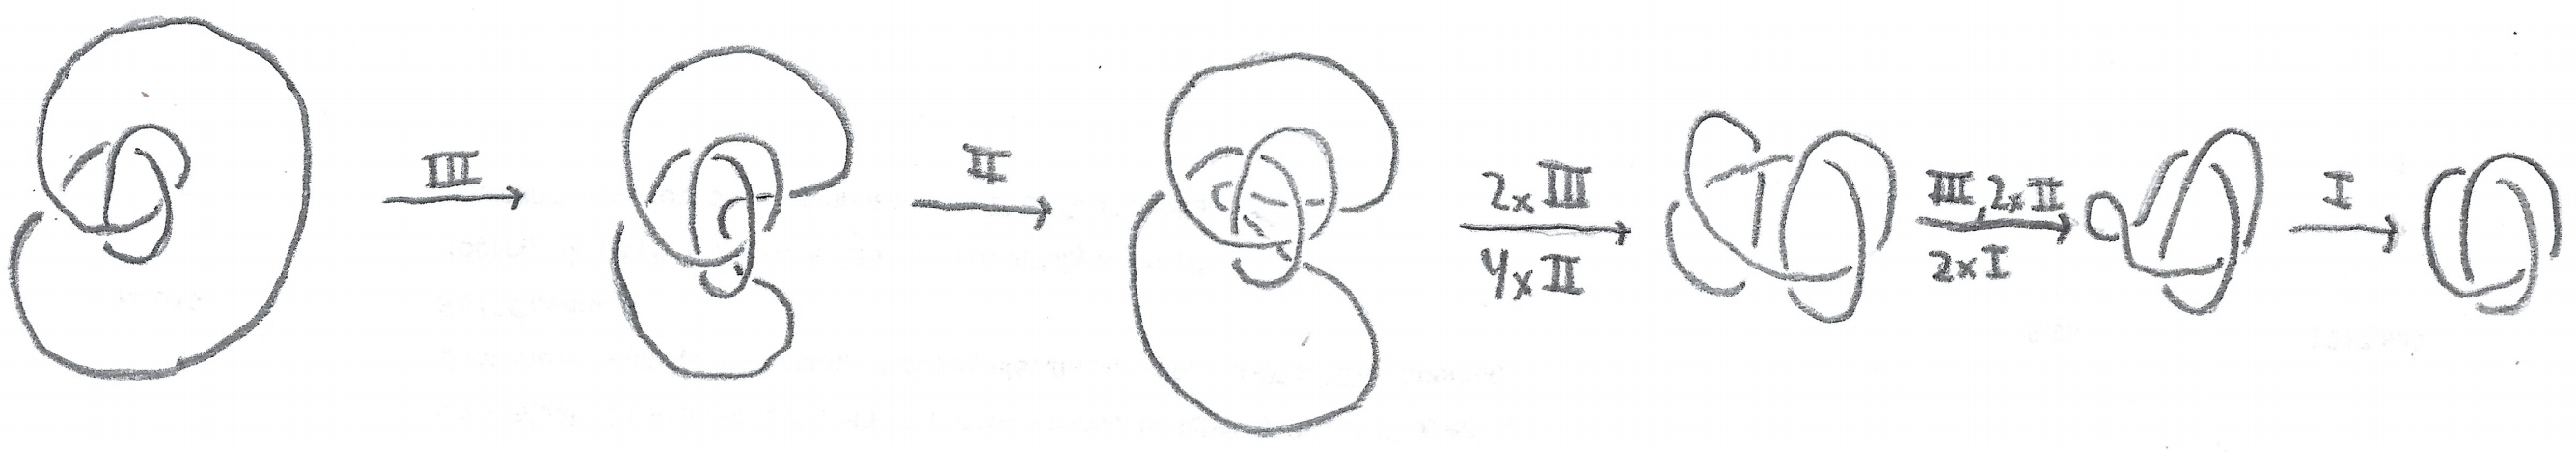
\includegraphics[width=0.8\linewidth]{Blender/ex1-10-2.png}
        \caption{Solution to \emph{Exercise 1.10}.}
        \label{fig:ex1-10-2}
    \end{figure}
    \item \emph{Exercise 1.11*}: Find a sequence of Reidemeister moves to untangle the unknot shown in Figure \ref{fig:ex1-11}.
    \begin{figure}[h!]
        \centering
        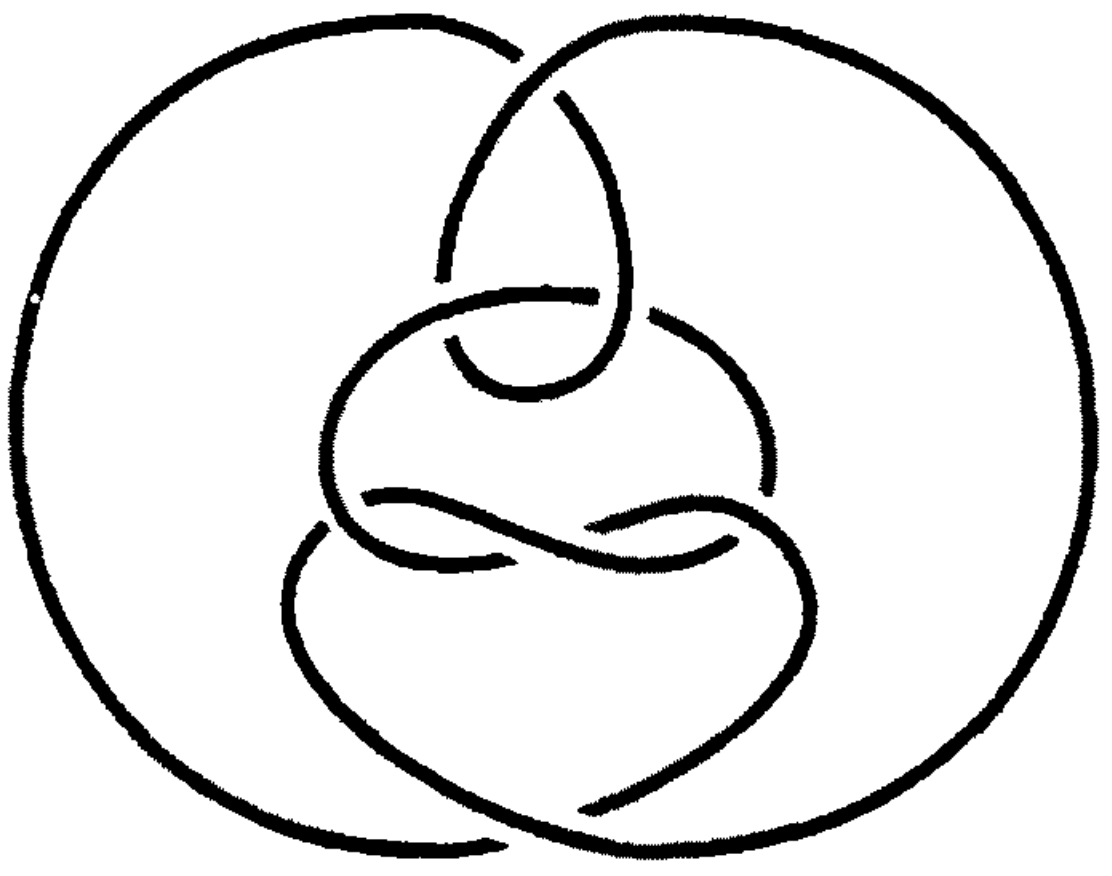
\includegraphics[width=0.17\linewidth]{Blender/ex1-11.png}
        \caption{Unknot to be untangled.}
        \label{fig:ex1-11}
    \end{figure}
    \begin{figure}[h!]
        \centering
        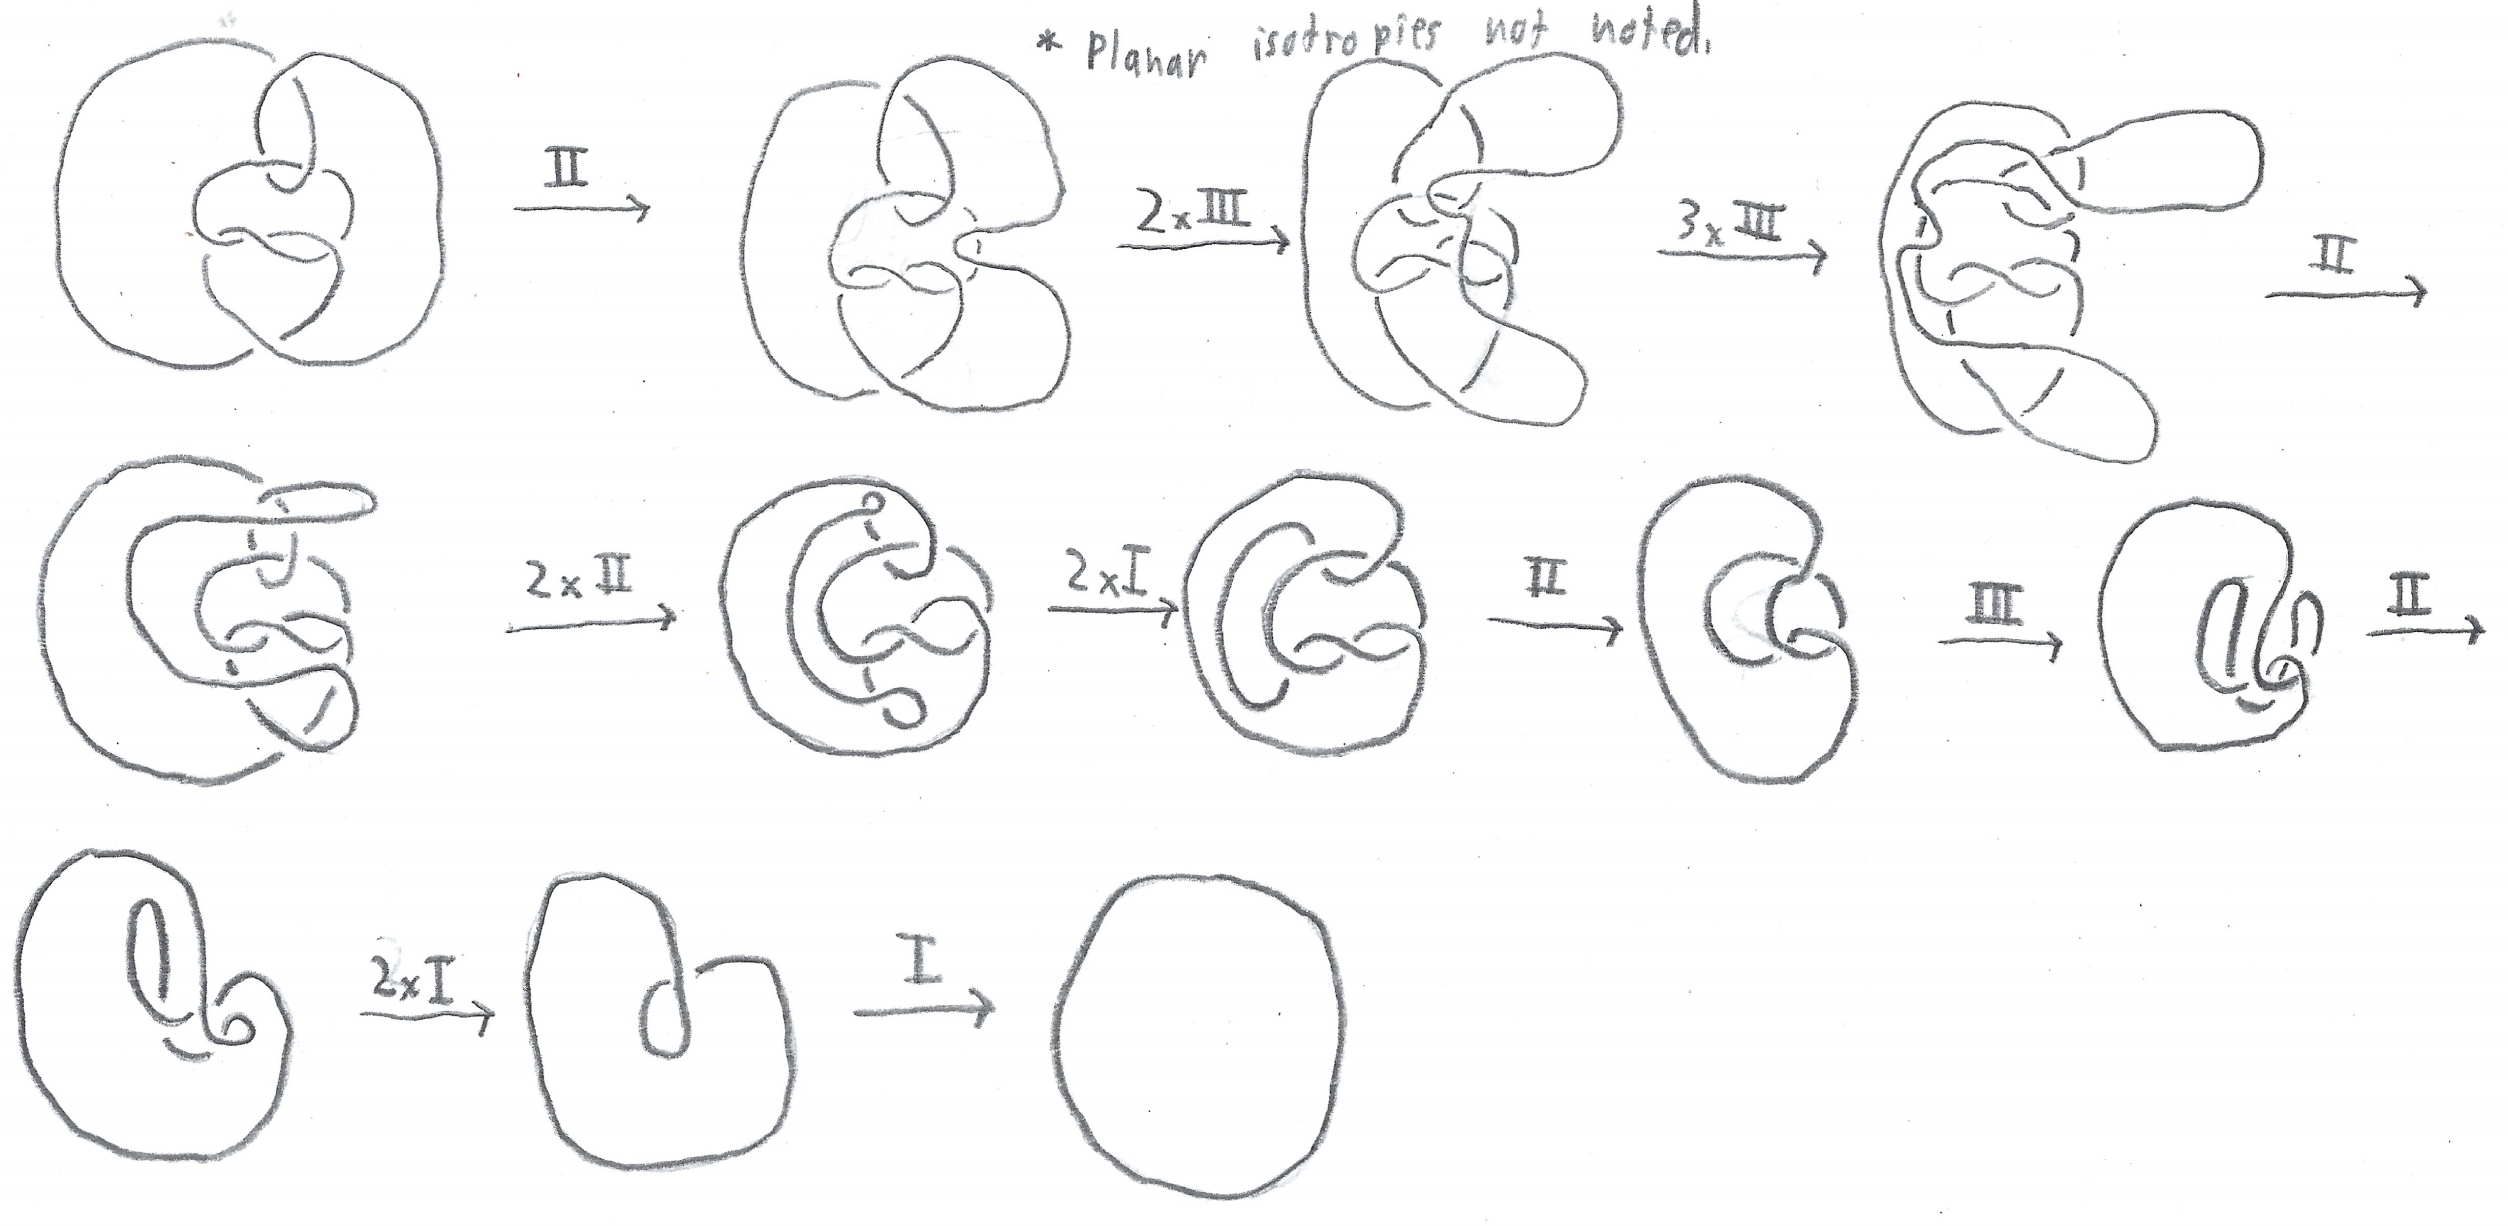
\includegraphics[width=0.8\linewidth]{Blender/ex1-11-2.png}
        \caption{Solution to \emph{Exercise 1.11*}.}
        \label{fig:ex1-11-2}
    \end{figure}
    \item The bounds on the increase in crossings generated by Reidemeister moves from one projection to another are unknown.
\end{itemize}


\subsection{Links}\label{sss:Links}
\begin{itemize}
    \item \textbf{Link}: \dq{A set of knotted loops all tangled up together}{17}
    \item \dq{Two links are considered to be the same if we can deform the one link to the other link without ever having any one of the loops intersect itself or any of the other loops in the process}{17}
    \begin{figure}[h!]
        \centering
        \begin{subfigure}[b]{0.2\linewidth}
            \centering
            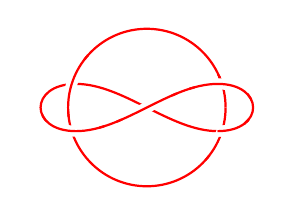
\begin{tikzpicture}
                \begin{knot}[
                    clip width=5,
                    ignore endpoint intersections=false,
                    consider self intersections=true
                ]
                    \strand[red,thick] circle (1cm);
                    \strand[red,thick] plot[smooth cycle,tension=1.2] coordinates{
                        (-0.9,0.3) (0.9,-0.3) (0.9,0.3) (-0.9,-0.3)
                    };
                    \flipcrossings{3,5}
                \end{knot}
            \end{tikzpicture}
            \caption{Whitehead link.}
            \label{fig:WhiteheadBorromeana}
        \end{subfigure}
        \begin{subfigure}[b]{0.2\linewidth}
            \centering
            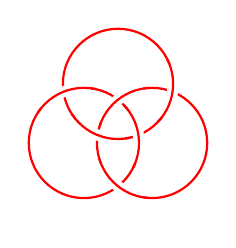
\begin{tikzpicture}
                \begin{knot}[
                    clip width=5
                ]
                    \strand[red,thick] (90:0.5)  circle (0.7cm);
                    \strand[red,thick] (210:0.5) circle (0.7cm);
                    \strand[red,thick] (330:0.5) circle (0.7cm);
                    \flipcrossings{1,2,5,6}
                \end{knot}
            \end{tikzpicture}
            \caption{Borromean rings.}
            \label{fig:WhiteheadBorromeanb}
        \end{subfigure}
        \caption{Projections of two common links.}
        \label{fig:WhiteheadBorromean}
    \end{figure}
    \item \emph{Exercise 1.13}: Show that the two projections in Figure \ref{fig:ex1-13a} and \ref{fig:ex1-13c} represent the same link.
    \begin{itemize}
        \item Untwist the right side of the figure-eight loop, twisting the right side of the circle at the same time. Then add a further twist to the circle loop and flip (rotate along the horizontal axis) the figure-eight loop (which now looks like an ellipse).
    \end{itemize}
    \begin{figure}[h!]
        \centering
        \begin{subfigure}[b]{0.3\linewidth}
            \centering
            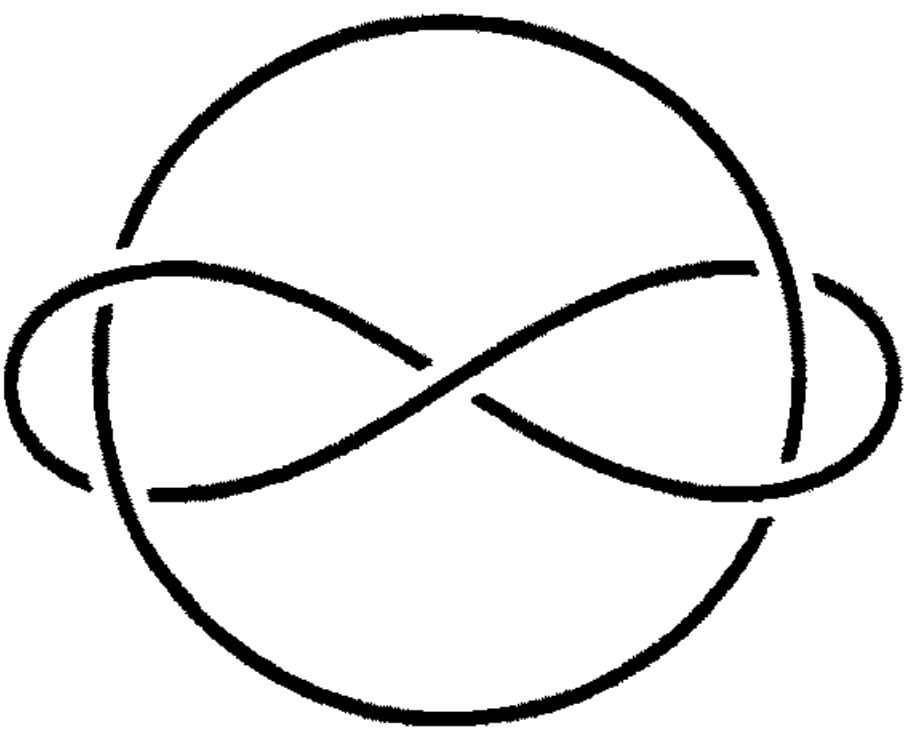
\includegraphics[width=0.5\linewidth]{Blender/ex1-13a.png}
            \caption{Initial projection.}
            \label{fig:ex1-13a}
        \end{subfigure}
        \begin{subfigure}[b]{0.3\linewidth}
            \centering
            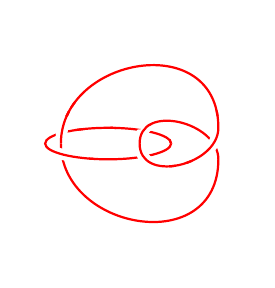
\begin{tikzpicture}
                \begin{knot}[
                    clip width=5,
                    consider self intersections=true,
                    ignore endpoint intersections=false
                ]
                    \strand[red,thick] (-0.4,0) ellipse (0.8cm and 0.2cm);
                    \strand[red,thick] (-1,0)
                        to [out=90,in=90,out looseness=1.4,in looseness=1.6] (1,0.2)
                        to [out=270,in=270,out looseness=1.2,in looseness=1.3] (0,0)
                        to [out=90,in=90,out looseness=1.3,in looseness=1.2] (1,-0.2)
                        to [out=270,in=270,out looseness=1.6,in looseness=1.4] cycle
                    ;
                    \flipcrossings{2,4,6}
                \end{knot}
            \end{tikzpicture}
            \vspace{-1em}
            \caption{Intermediate projection.}
            \label{fig:ex1-13b}
        \end{subfigure}
        \begin{subfigure}[b]{0.3\linewidth}
            \centering
            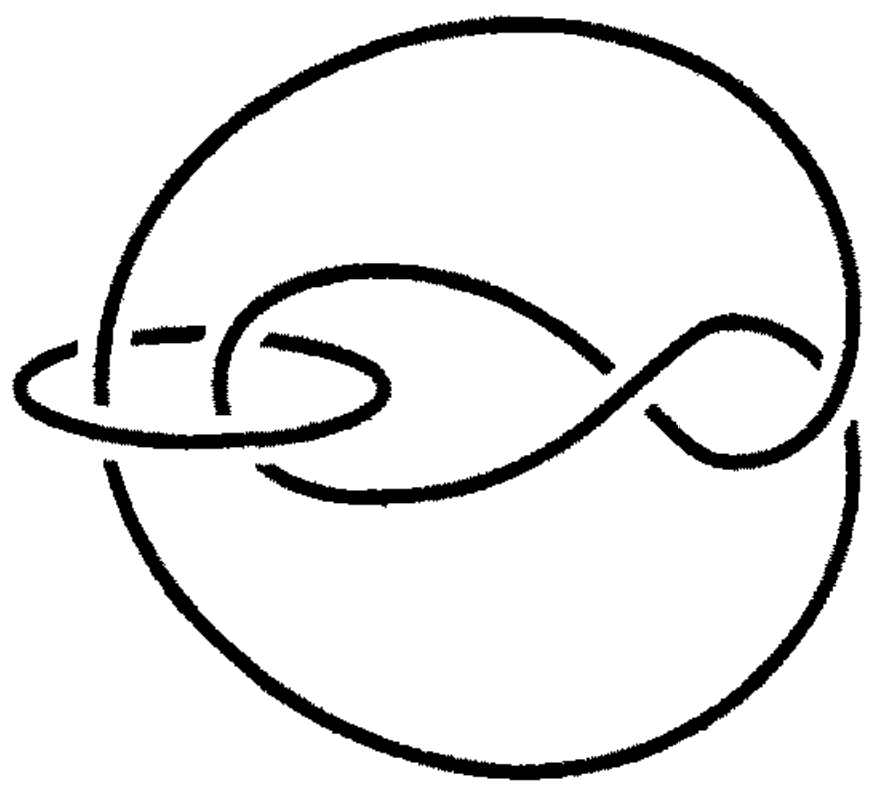
\includegraphics[width=0.5\linewidth]{Blender/ex1-13c.png}
            \caption{Final projection.}
            \label{fig:ex1-13c}
        \end{subfigure}
        \caption{Ambient isotropies of the Whitehead link.}
        \label{fig:ex1-13}
    \end{figure}
    \item \textbf{Link of \emph{n} components}: A link made up of $n$ loops knotted with each other.
    \begin{itemize}
        \item The Whitehead link (Figure \ref{fig:WhiteheadBorromeana}) is a \underline{link of 2 components}.
        \item The Borromean rings (Figure \ref{fig:WhiteheadBorromeanb}) are a \underline{link of 3 components}.
        \item A knot is a \underline{link of 1 component}.
        \item If the number of components in two links differ, then the links are clearly distinct.
    \end{itemize}
    \item \textbf{Splittable}: A link whose components \dq{can be deformed so that they lie on different sides of a plane in three-space}{17}
    \item \emph{Exercise 1.14}: Show that the link in Figure \ref{fig:ex1-14} is splittable.
    \begin{figure}[h!]
        \centering
        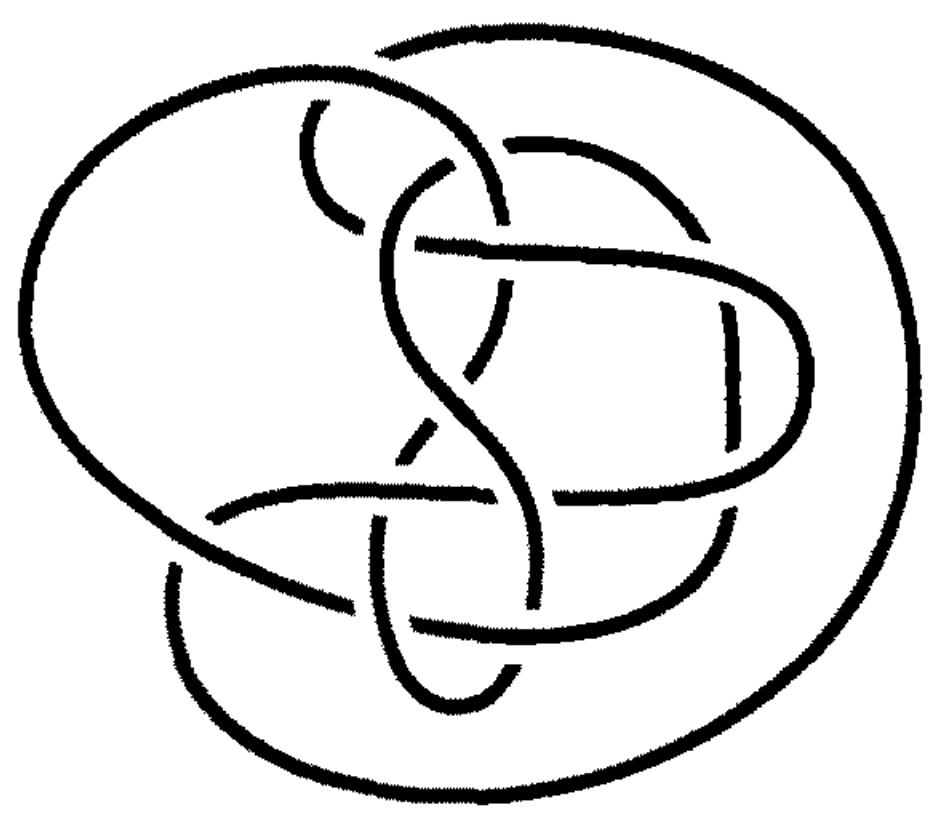
\includegraphics[width=0.2\linewidth]{Blender/ex1-14.png}
        \caption{Link to be split.}
        \label{fig:ex1-14}
    \end{figure}
    \begin{figure}[h!]
        \centering
        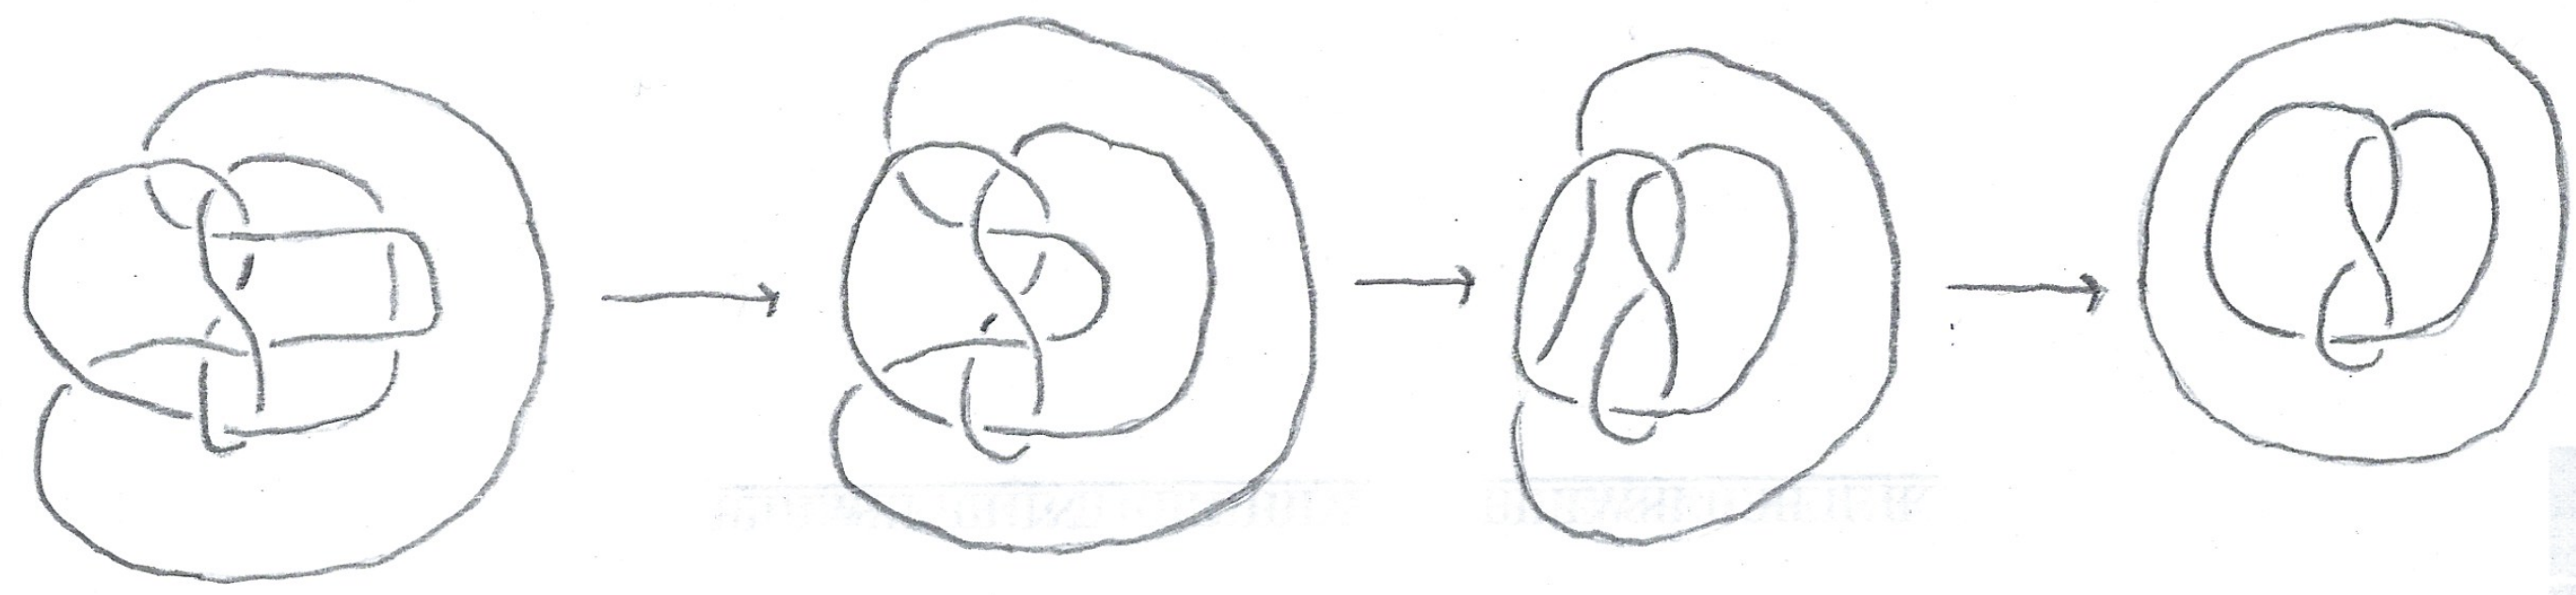
\includegraphics[width=0.8\linewidth]{Blender/ex1-14-2.png}
        \caption{Solution to \emph{Exercise 1.14}.}
        \label{fig:ex1-14-2}
    \end{figure}
    \item \textbf{Unlink}: One of the two simplest links of two components and the simplest splittable link of two components. \emph{Also known as} \textbf{trivial link}. See Figure \ref{fig:unlinkHopfa}.
    \item \textbf{Hopf link} The other of the two simplest links of two components and the simplest nonsplittable link of two components. See Figure \ref{fig:unlinkHopfb}.
    \begin{figure}[h!]
        \centering
        \begin{subfigure}[b]{0.4\linewidth}
            \centering
            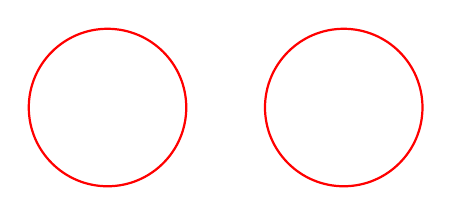
\begin{tikzpicture}[red,thick]
                \draw (-1.5,0) circle (1cm);
                \draw (1.5,0)  circle (1cm);
            \end{tikzpicture}
            \caption{Trivial link.}
            \label{fig:unlinkHopfa}
        \end{subfigure}
        \begin{subfigure}[b]{0.4\linewidth}
            \centering
            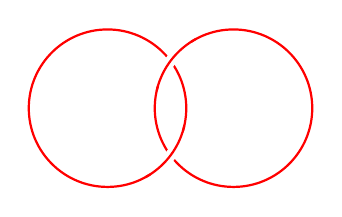
\begin{tikzpicture}
                \begin{knot}[
                    clip width=5,
                    flip crossing=1
                ]
                    \strand[red,thick] (-0.8,0) circle (1cm);
                    \strand[red,thick] (0.8,0)  circle (1cm);
                \end{knot}
            \end{tikzpicture}
            \caption{Hopf link.}
            \label{fig:unlinkHopfb}
        \end{subfigure}
        \caption{Projections of the two simplest links of two components.}
        \label{fig:unlinkHopf}
    \end{figure}
    \item \textbf{Linking number}: A quantity that numerically measures how linked up two components are.
    \begin{itemize}
        \item If $M$ and $N$ are two components in a link, begin by orienting both of them.
        \item At each crossing, count a $+1$ if Figure \ref{fig:linkingnumbera} holds or count a $-1$ if Figure \ref{fig:linkingnumberb} holds.
        \begin{itemize}
            \item Note that if you are unsure, do the following: If rotating the bottom strand clockwise lines up the arrows (correlates the two orientations), count $+1$.
            \item In the same vein, if rotating the bottom strand counterclockwise lines up the arrows, count $-1$.
            \item If a component crosses itself, do not count it.
        \end{itemize}
        \begin{figure}[h!]
            \centering
            \begin{subfigure}[b]{0.2\linewidth}
                \centering
                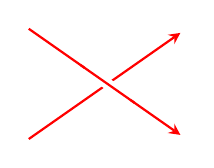
\begin{tikzpicture}
                    \begin{knot}[
                        clip width=5,
                        flip crossing=1
                    ]
                        \strand[red,thick,-stealth] (-1,-0.7) -- (1,0.7);
                        \strand[red,thick,-stealth] (-1,0.7) -- (1,-0.7);
                    \end{knot}
                \end{tikzpicture}
                \caption{Count $+1$.}
                \label{fig:linkingnumbera}
            \end{subfigure}
            \begin{subfigure}[b]{0.2\linewidth}
                \centering
                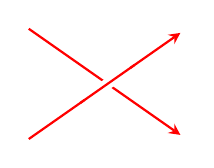
\begin{tikzpicture}
                    \begin{knot}[
                        clip width=5
                    ]
                        \strand[red,thick,-stealth] (-1,-0.7) -- (1,0.7);
                        \strand[red,thick,-stealth] (-1,0.7) -- (1,-0.7);
                    \end{knot}
                \end{tikzpicture}
                \caption{Count $-1$.}
                \label{fig:linkingnumberb}
            \end{subfigure}
            \caption{Computing linking numbers per crossing.}
            \label{fig:linkingnumber}
        \end{figure}
        \item Sum all of the $+1$s and $-1$s and divide this sum by 2 to yield the linking number.
        \begin{itemize}
            \item For example, the linking number for the Hopf link (Figure \ref{fig:unlinkHopfb}) is $\pm 1$ depending on the chosen orientation.
            \item Note that reversing the orientation for one of the two links is equivalent to multiplying the linking number by $-1$.
            \item As such, the absolute value of the linking number remains constant whatever orientation is chosen.
        \end{itemize}
    \end{itemize}
    \item \emph{Exercise 1.15}: Compute the linking number of the link pictured in Figure \ref{fig:ex1-15}. Now reverse the direction on one of the components and recompute it.
    \begin{itemize}
        \item Add up all of the numbers in the second row of Table \ref{tab:ex1-15} to yield $2$. Divide by $2$ to yield the linking number, $1$.
    \end{itemize}
    \begin{figure}[h!]
        \centering
        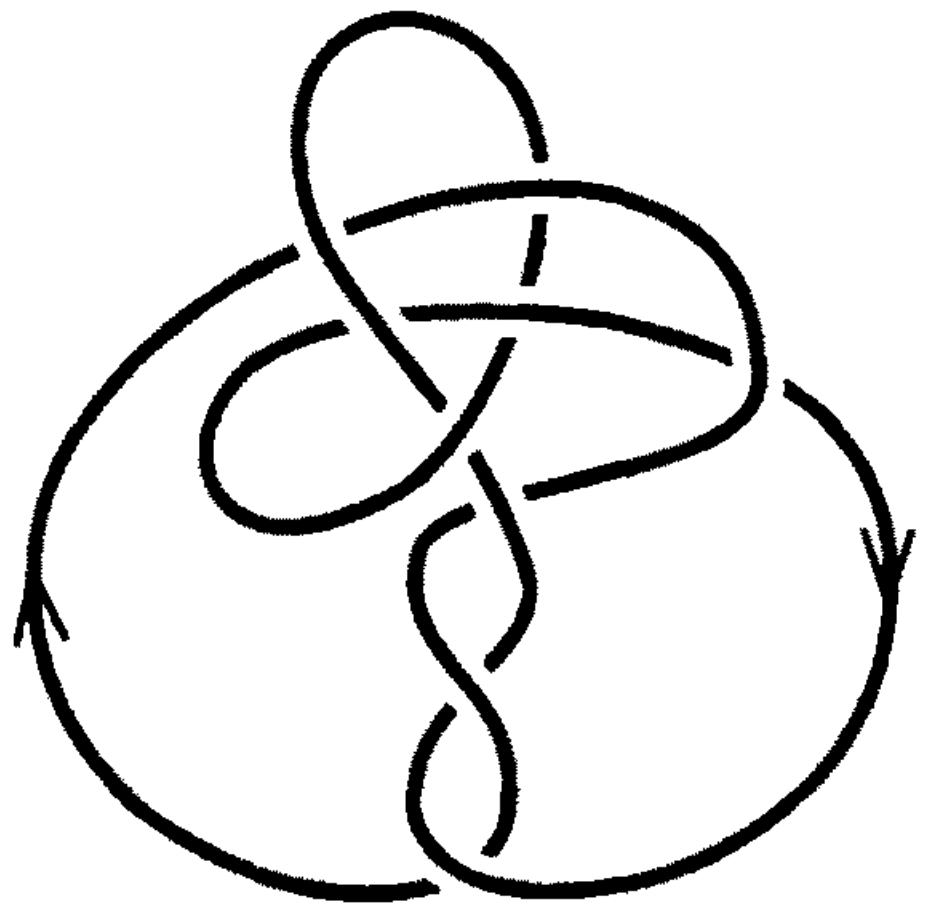
\includegraphics[width=0.2\linewidth]{Blender/ex1-15.png}
        \begin{tikzpicture}[
                remember picture,overlay,
                red,thin
            ]
            \draw (-1.5,2.6)   circle (4pt) node[right]{A};
            \draw (-2.28,2.42) circle (4pt) node[left] {B};
            \draw (-2.08,2.13) circle (4pt) node[left] {C};
            \draw (-1.56,2.16) circle (4pt) node[right]{D};
            \draw (-0.73,1.96) circle (4pt) node[right]{E};
            \draw (-1.78,1.76) circle (4pt) node[right]{F};
            \draw (-1.65,1.48) circle (4pt) node[right]{G};
            \draw (-1.74,0.83) circle (4pt) node[right]{H};
            \draw (-1.77,0.15) circle (4pt) node[right]{I};
        \end{tikzpicture}
        \caption{Link of linking number $n$.}
        \label{fig:ex1-15}
    \end{figure}
    \renewcommand{\arraystretch}{1.4}
    \begin{table}[h!]
        \centering
        \begin{tabular}{|c|c|c|c|c|c|c|c|c|}
            \hline
            A    & B    & C   & D   & E    & F   & G    & H    & I   \\
            \hline
            $-1$ & $-1$ & $0$ & $0$ & $+1$ & $0$ & $+1$ & $+1$ & $+1$\\
            \hline
        \end{tabular}
        \caption{Counting crossings.}
        \label{tab:ex1-15}
    \end{table}
    \item Although a linking number is computed using a single projection of a link, the linking number will be the same for any projection of the link.
    \begin{itemize}
        \item This can be proven by demonstrating that the Redemeister moves do not change the linking number. \dq{Since we can get from any one projection of a link to any other via a sequence of Reidemeister moves, none of which will change the linking number, it must be that two different projections of the same link yield the same linking number}{20}
        \item Let's take this case by case.
        \begin{itemize}
            \item A Type I Reidemeister move generates a self-intersection. Because self-crossings do not count toward the linking number by definition, the first Reidemeister move does not affect the linking number.
            \item A Type II Reidemeister move generates two crossings. There are now two cases: Either the new crossings are self-intersections or they are not. If the new crossings are self-intersections, then there is no change to the linking number. If the new crossings are not self-intersections, they will always have opposite linking numbers, and, thus, the two new crossings cancel each other out. Therefore, the second Reidemeister move does not affect the linking number.
            \item A Type III Reidemeister move removes two crossings and generates two crossings. There are now two cases: Either the new crossings are self-intersections or they are not. If the new crossings are self-intersections, then there is no change to the linking number. If the new crossings are not self-intersections, both pairs of crossings will always have opposite linking numbers and, thus, both pairs of crossings cancel each other out. Therefore, the third Reidemeister move does not affect the linking number.
        \end{itemize}
        \item This logic can be visually confirmed by assigning orientations and counting crossings in Figure \ref{fig:reidem}.
    \end{itemize}
    \item \textbf{Invariant}: A quality of a knot or link that, once orientations are chosen, is unchanged by ambient isotropy.
    \begin{itemize}
        \item Both the linking number and the number of components are \underline{link invariants}.
    \end{itemize}
    \item \emph{Exercise 1.16}: Explain why the linking number of a splittable two-component link will always be $0$, no matter what projection is used to compute it.
    \begin{itemize}
        \item \textsc{Solution 1}: By definition, the linking number numerically measures how linked up two components are. Since splittable links are not joined (or "linked up") in any way, the linking number must be $0$.
        \item \textsc{Solution 2}: If a two-component link is splittable, then there exists a projection of it with no crossings that are not self-intersections (a projection of the split link, as in Figure \ref{fig:unlinkHopfb}). If all crossings are self-intersections, then the linking number computed for this projection must be $0$. Now that it is known that said link has a linking number of $0$, any combination of Reidemeister moves can be used to manipulate the link into any other projection. But because Reidemeister moves do not affect the linking number, the linking number will remain $0$.
    \end{itemize}
    \item The absolute value of the linking number, as a link invariant, can be used to distinguish certain distinct links, regardless of orientation.
    \begin{itemize}
        \item \dq{Any two links with two components that have distinct absolute values of their linking numbers have to be different links}{21}
        \item For example, the difference in linking number between the unlink (0; Figure \ref{fig:unlinkHopfa}) and the Hopf link (1; Figure \ref{fig:unlinkHopfb}) distinguishes them.
    \end{itemize}
    \item However, the linking number cannot distinguish between all links.
    \begin{itemize}
        \item For instance, both the Whitehead link (Figure \ref{fig:WhiteheadBorromeana}) and the unlink (Figure \ref{fig:unlinkHopfa}) have linking number 0.
        \item One such distinction is discussed in Section \ref{sss:tricolor}.
    \end{itemize}
    \item \textbf{Brunnian link}: A nontrivial link where the removal of any one component leaves behind a set of trivial unlinked circles.
    \begin{itemize}
        \item The Borromean rings (Figure \ref{fig:WhiteheadBorromeanb}) are Brunnian$^[$\footnote{How can I draw a Brunnian link with four components? Or more?}$^]$.
    \end{itemize}
\end{itemize}


\subsection{Tricolorability}\label{sss:tricolor}
\begin{itemize}
    \item How do we \emph{prove} that every knot is not just a projection of the unknot?
    \item \textbf{Strand}: \dq{A piece of the link that goes from one undercrossing to another with only overcrossings in between}{23}
    \item \textbf{Tricolorable}: A projection of a knot or link in which each strand \dq{can be colored one of three different colors, so that at each crossing, either three different colors come together or all the same color comes together}{23}
    \begin{figure}[h!]
        \centering
        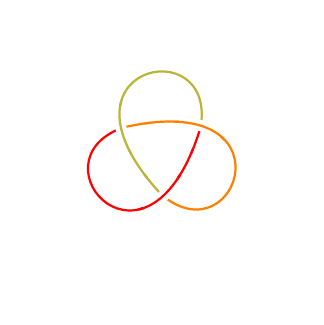
\begin{tikzpicture}
            \coordinate (a) at (30:0.57);
            \coordinate (b) at (150:0.57);
            \coordinate (c) at (270:0.57);
        
            \begin{knot}[
                clip width=5,clip radius=8pt,ignore endpoint intersections=false
            ]
                \strand[red,thick] (a) to[relative,out=73,in=20,out looseness=5.8,in looseness=3.3] (b);
                \strand[orange,thick] (b) to[relative,out=73,in=20,out looseness=5.8,in looseness=3.3] (c);
                \strand[yellow!70!black,thick] (c) to[relative,out=73,in=20,out looseness=5.8,in looseness=3.3] (a);
                \flipcrossings{1,3,5}
                \redraw{1}{(c)}
            \end{knot}
        \end{tikzpicture}
        \vspace{-0.8cm}
        \caption{Tricolored trefoil.}
        \label{fig:TricolorTrefoil}
    \end{figure}
    \item \emph{Exercise 1.21}: Determine which of the projections of the three six-crossing knots $6_1$, $6_2$, and $6_3$ are tricolorable.
    \begin{itemize}
        \item $6_1$ is tricolorable and the other two knots are not. I determined this through trial and error.
    \end{itemize}
    \item \emph{Exercise 1.22}: Show that the projection of the knot $7_4$ in Figure \ref{fig:ex1-22a} is tricolorable.
    \begin{figure}[h!]
        \centering
        \begin{subfigure}[b]{0.3\linewidth}
            \centering
            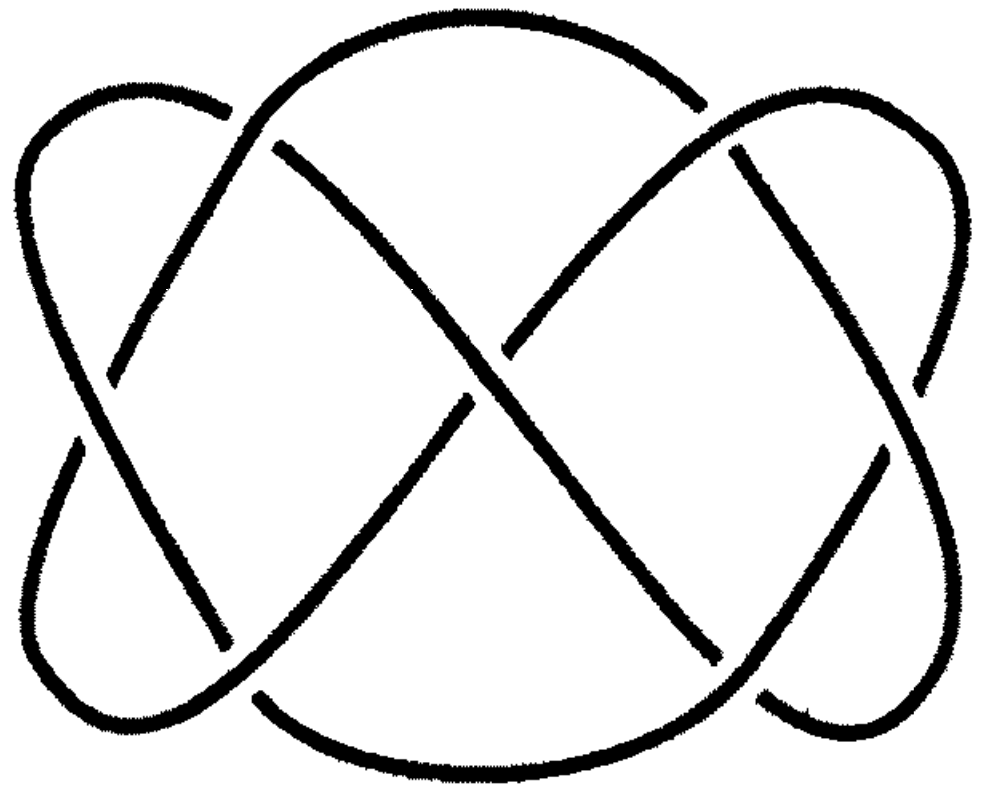
\includegraphics[width=0.5\linewidth]{Blender/ex1-22.png}
            \caption{Initial projection.}
            \label{fig:ex1-22a}
        \end{subfigure}
        \begin{subfigure}[b]{0.3\linewidth}
            \centering
            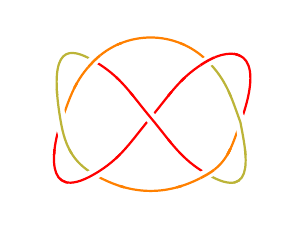
\begin{tikzpicture}[scale=0.6]
                \coordinate (a) at (-1.2,0.5);
                \coordinate (b) at (1.2,0.5);
                \coordinate (c) at (1.9,1.6);
                \coordinate (d) at (1.2,2.9);
                \coordinate (e) at (0,1.7);
                \coordinate (f) at (-1.9,1.6);
                \coordinate (g) at (-1.2,2.9);
                
                \begin{knot}[
                    clip width=5,
                    ignore endpoint intersections=false
                ]
                    \strand[orange,thick] (a)
                        to [out=-30,in=-150] (b)
                        to [out=30,in=-110] (c)
                    ;
                    \strand[red,thick] (c)
                        to [out=70,in=30,out looseness=3] (d)
                        to [out=-150,in=50] (e)
                    ;
                    \strand[red,thick] (e)
                        to [out=-130,in=30] (a)
                        to [out=-150,in=-110,out looseness=2.5] (f)
                    ;
                    \strand[orange,thick] (f)
                        to [out=70,in=-135] (g)
                        to [out=45,in=135] (d)
                    ;
                    \strand[yellow!70!black,thick] (d)
                        to [out=-45,in=110] (c)
                        to [out=-80,in=-30,in looseness=2.5] (b)
                    ;
                    \strand[red,thick] (b)
                        to [out=150,in=-50] (e)
                        to [out=130,in=-30] (g)
                    ;
                    \strand[yellow!70!black,thick] (g)
                        to [out=150,in=100,in looseness=3] (f)
                        to [out=-80,in=150] (a)
                    ;
                    \flipcrossings{10,13,19}
                \end{knot}

                \begin{scope}
                    \path[clip] (b) circle (5pt);
                    \draw[white,double=orange,very thick,double distance=0.9pt] (a)
                        to [out=-30,in=-150] (b)
                        to [out=30,in=-110] (c)
                    ;
                \end{scope}
                \begin{scope}
                    \path[clip] (d) circle (5pt);
                    \draw[white,double=red,very thick,double distance=0.9pt] (c)
                        to [out=70,in=30,out looseness=3] (d)
                        to [out=-150,in=50] (e)
                    ;
                \end{scope}
                \begin{scope}
                    \path[clip] (g) circle (5pt);
                    \draw[white,double=orange,very thick,double distance=0.9pt] (f)
                        to [out=70,in=-135] (g)
                        to [out=45,in=135] (d)
                    ;
                \end{scope}
            \end{tikzpicture}
            \caption{Tricolored projection.}
            \label{fig:ex1-22b}
        \end{subfigure}
        \caption{Tricolored $7_4$.}
        \label{fig:ex1-22}
    \end{figure}
    \item Reidemeister moves do not affect tricolorability.
    \begin{itemize}
        \item A Type I Reidemeister move generates a self-intersection. At such a crossing (made out of one original strand), every color will be the same; only one color meets at the crossing.
        \item A Type II Reidemeister move generates two crossings. If the strands are the same color, then everything stays the same color. If the strands are different colors, than newly created loop takes on the third color.
        \item Type III has many cases (\emph{Exercise 1.23}).
    \end{itemize}
    \item Since the unknot is not tricolorable and the trefoil knot is, we have just proven that there is at least one other knot besides the unknot.
    \begin{itemize}
        \item Tricolorability is a knot invariant.
    \end{itemize}
    \item For links, tricolorability is a bit different --- the unlink, for example, is tricolorable.
    \begin{figure}[h!]
        \centering
        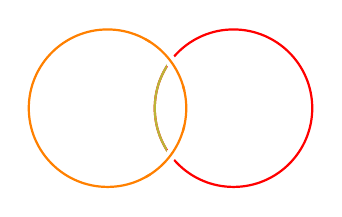
\begin{tikzpicture}
            \begin{knot}[
                clip width=5
            ]
                \strand[orange,thick] (-0.8,0) circle (1cm);
                \strand[red,thick] (0.8,0)  circle (1cm);
            \end{knot}
            \begin{scope}
                \clip (-0.045,-1) rectangle (-1.8,1);
                \draw[yellow!70!black,thick] (0.8,0) circle (1cm);
            \end{scope}
        \end{tikzpicture}
        \caption{Tricolored unlink.}
        \label{fig:tricolorUnlink}
    \end{figure}
\end{itemize}


\subsection{Knots and Sticks}\label{sss:KnotsSticks}
\begin{itemize}
    \item We can also consider knots made out of straight sticks glued to each other at each end.
    \item The first nontrivial knot made out of sticks is the trefoil, with six sticks.
    \begin{itemize}
        \item We know that the stick trefoil in Figure \ref{fig:sticktrefoil} could be made in the real world because, if two vertices lie in the $xy$-plane, then two lie above and two lie below.
        \item This P(lanar), L(ow), H(igh) notation is commonly used.
    \end{itemize}
    \begin{figure}[h!]
        \centering
        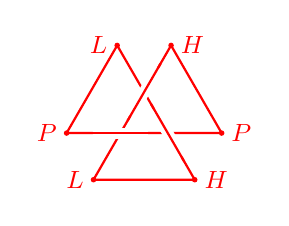
\begin{tikzpicture}
            \begin{knot}[
                clip width=5,
                consider self intersections
            ]
                \strand[red,thick] (70:1) to (-10:1) to (-170:1) to (110:1) to (-50:1) to (-130:1) to cycle;
                \flipcrossings{1,3}
            \end{knot}

            \fill[red] (70:1)   circle (1pt) node[right]{\small$H$};
            \fill[red] (-10:1)  circle (1pt) node[right]{\small$P$};
            \fill[red] (-170:1) circle (1pt) node[left] {\small$P$};
            \fill[red] (110:1)  circle (1pt) node[left] {\small$L$};
            \fill[red] (-50:1)  circle (1pt) node[right]{\small$H$};
            \fill[red] (-130:1) circle (1pt) node[left] {\small$L$};
        \end{tikzpicture}
        \caption{A trefoil knot made of sticks.}
        \label{fig:sticktrefoil}
    \end{figure}
    \item \textbf{Stick number}: \dq{The least number of straight sticks necessary to make a knot $K$}{29} \emph{Also known as} \textbf{s(K)}.
    \item The stick number for the composition of $n$ trefoil knots is $2n+4$.
    \item Many problems listed$^[$\footnote{These could make good topics for a larger paper. Alternatively, some I am not ready to solve and need to learn more math first (those that I will come back to at the end of the book). I do not believe I'm missing anything essential by skipping these for now, but we'll see.}$^]$.
\end{itemize}
\newpage



\section{Tabulating Knots}\label{sse:tabulating}
\subsection{History of Knot Tabulation}
\begin{itemize}
    \item Although many mathematicians (including Gauss) had dabbled with knots, Lord Kelvin's theory that atoms were knotted vortices in the ether (referenced in Section \ref{sss:Introduction}) kicked off research in earnest.
    \item Reverend Thomas P. Kirkman began tabulating knots but wrote poorly.
    \item However, Kirkman's ideas were applied by Scottish physicist Peter Guthrie Tait to list all alternating knots up to 10 crossings.
    \item C. N. Little of the University of Nebraska was the first to tackle the nonalternating knots.
    \begin{itemize}
        \item He tabulated up to 10 crossings (43 knots total).
        \item However, in 1974, it was discovered that two knots were, in fact, the same and there were really 42 knots.
        \begin{itemize}
            \item Kenneth A. Perko, a part time mathematician and New York lawyer, discovered that the projections were not distinct. As such, the projections are known as the Perko pair (Figure \ref{fig:perkopair}).
        \end{itemize}
    \end{itemize}
    \item \emph{Exercise 2.1}: Show that the Perko pair (projected in Figure \ref{fig:perkopair}) are the same knot.
    \begin{figure}[h!]
        \centering
        \begin{subfigure}[b]{0.2\linewidth}
            \centering
            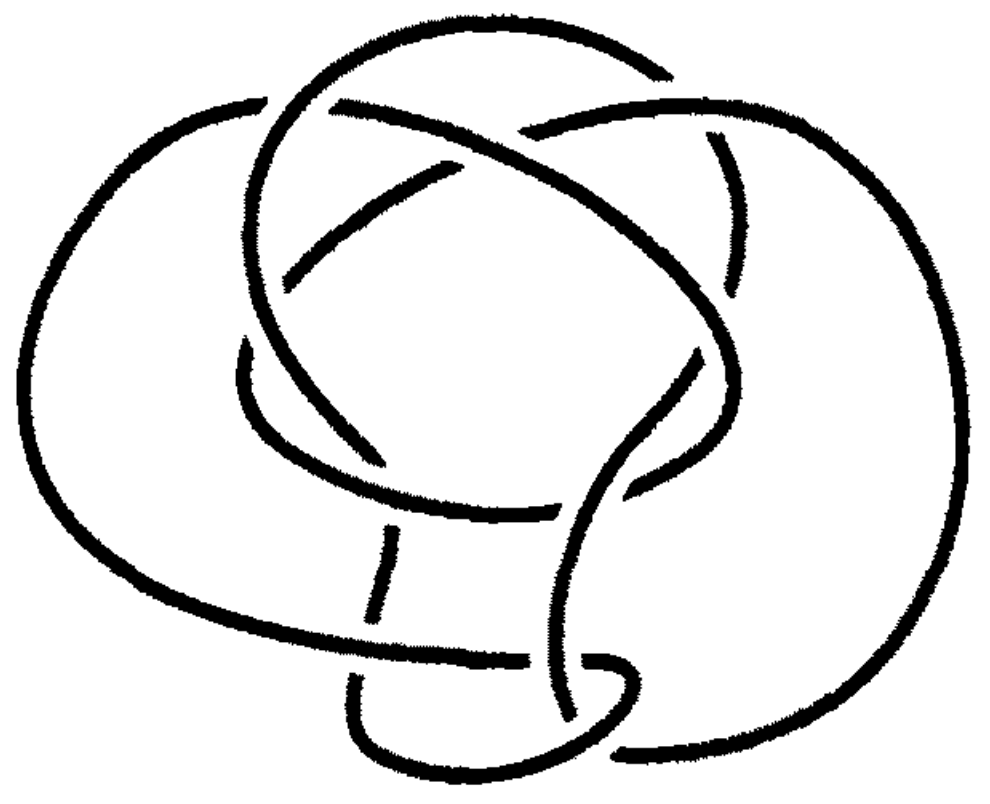
\includegraphics[width=0.8\linewidth]{Blender/perkopair1.png}
            \caption{Projection 1.}
            \label{fig:perkopaira}
        \end{subfigure}
        \begin{subfigure}[b]{0.2\linewidth}
            \centering
            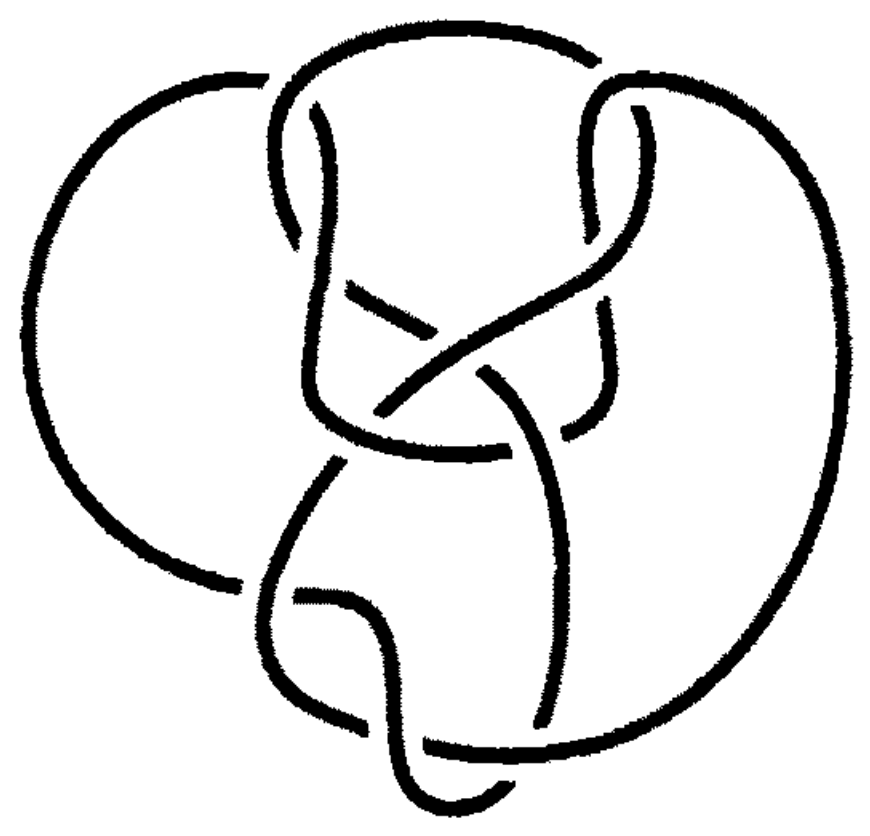
\includegraphics[width=0.7\linewidth]{Blender/perkopair2.png}
            \caption{Projection 2.}
            \label{fig:perkopairb}
        \end{subfigure}
        \caption{The Perko pair.}
        \label{fig:perkopair}
    \end{figure}
    \begin{figure}[h!]
        \centering
        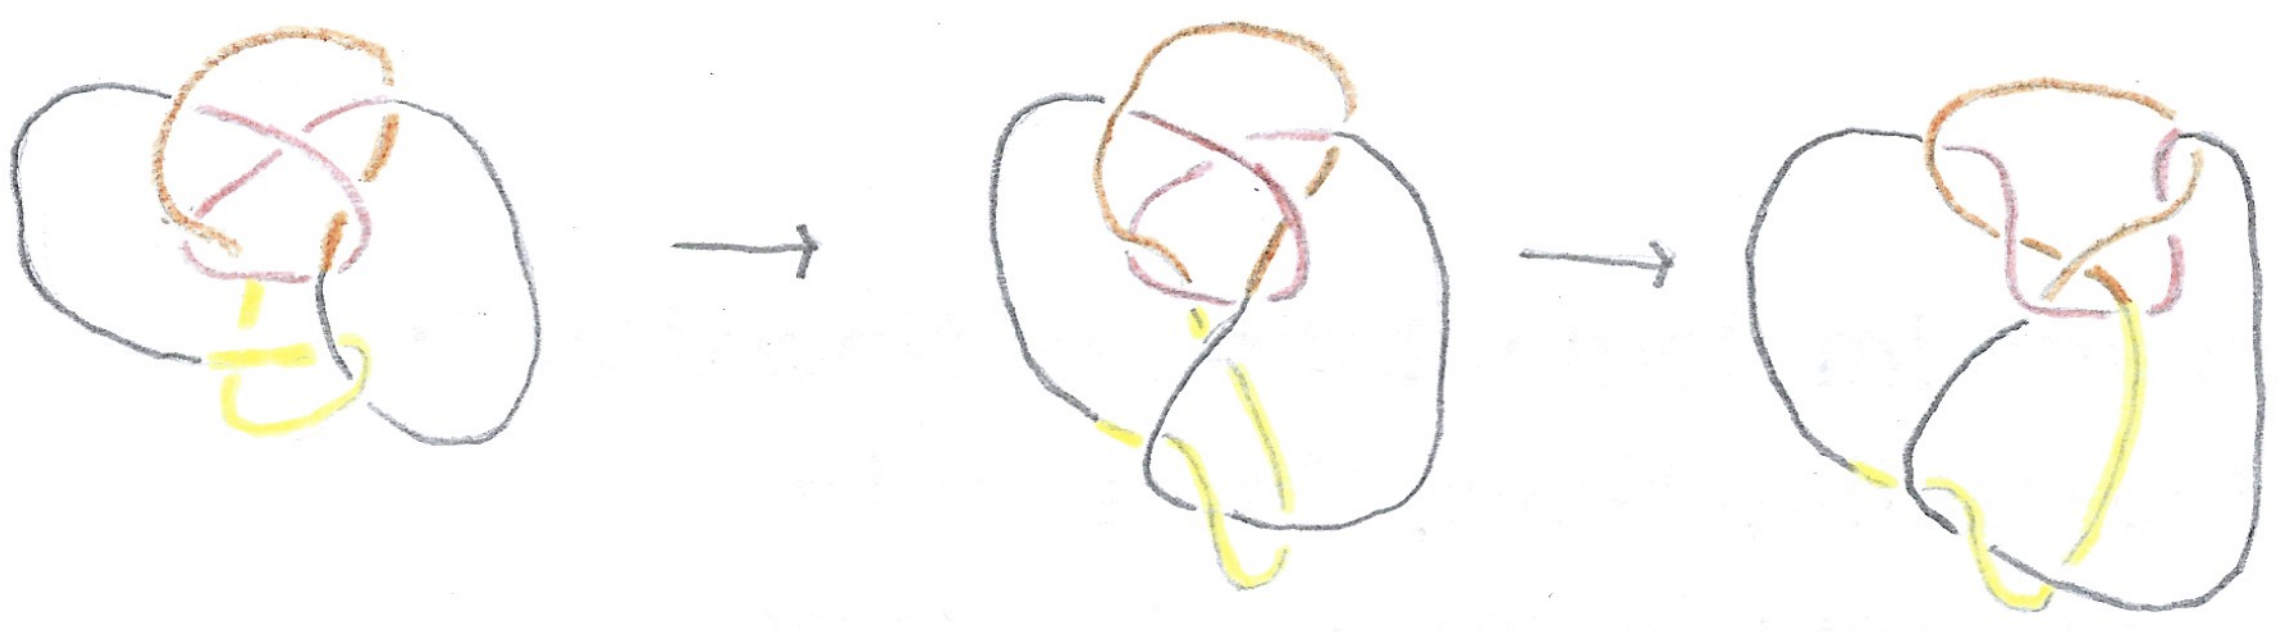
\includegraphics[width=0.6\linewidth]{Blender/ex2-1.png}
        \caption{Solution to \emph{Exercise 2.1}.}
        \label{fig:ex2-1}
    \end{figure}
    \item Little later published a census of 11-crossing alternating knots with 11 omissions and 1 duplication.
    \item Mary G. Haseman listed all amphicheiral knots of 12 crossings.
    \item Early on, there were few attempts to \emph{prove} that the tabulated knots were actually distinct.
    \item In 1927, Alexander and Briggs proved that the knots up to 9 crossings were distinct.
    \begin{itemize}
        \item They developed the first knot polynomial, the Alexander polynomial.
        \item This would remain the only knot polynomial until 1984.
    \end{itemize}
    \item Once Kurt Reidemeister finished rigorously classifying the knots up to 9 crossings in 1932, tabulation was inactive for a while.
    \item In 1969, John H. Conway developed a new notation and used it to determine all of the prime knots up to 11 crossings and all prime nonsplittable links up to 10 crossings.
    \item In 1978, Alain Caudron of the University of Paris corrected Conway's tabulation a bit.
    \item Meanwhile, a new notation was developed by Hugh Dowker (see Section \ref{sss:Dowker}) that was implemented as a computer algorithm by Morwen Thistlethwaite.
    \item In the 1980s-1990s (with computer help), Jim Hoste, Thistlethwaite, and Jeff Weeks (an expert in hyperbolic knots; see Section \ref{sss:Hyperbolic}) tabulated up to 16-crossing knots.
    \begin{itemize}
        \item Note that the number of knots of successive numbers of crossings \emph{appears} to grows exponentially (this is unproven).
        \item Also note that Hoste et al's listed knots includes those that are not amphicheiral only once, so those knots actually represent 2 distinct knots.
        \begin{itemize}
            \item Determining amphicheirality is discussed in Section \ref{sse:polynomials}
        \end{itemize}
    \end{itemize}
    \item On drawing a 14-crossing knot.
    \item Claus Ernst and Dewitt Sumners proved a lower exponential bound on the number of distinct prime knots (see Section \ref{sss:Bridge}).
    \item Dominic Welsh proved an upper exponential bound on the number of distinct prime knots.
\end{itemize}


\subsection{The Dowker Notation for Knots}\label{sss:Dowker}
\begin{itemize}
    \item For alternating knots\dots
    \begin{itemize}
        \item Begin by choosing an orientation.
        \item Label an arbitrary crossing 1.
        \item Leaving that crossing on the understrand, label the next crossing 2.
        \item Continue through the crossing on the same strand and label the next crossing 3.
        \item Continue in this fashion until you have gone all the way around the knot once.
        \begin{itemize}
            \item Note that this gives each crossing two numbers.
        \end{itemize}
    \end{itemize}
    \begin{figure}[h!]
        \centering
        \begin{tikzpicture}
            \begin{knot}[
                clip width=5,
                consider self intersections
            ]
                \strand[red,thick,
                decoration={markings,
                mark=at position 0.2 with {\arrow{>}}},
                postaction={decorate}] (90:1)
                    \foreach \x in {1,2,3} {
                        to [bend left=117,looseness=1.9] ({90+120*\x}:1)
                    }
                ;
                \flipcrossings{1,3}
            \end{knot}
            \footnotesize
            \fill (30:0.57) circle (0pt)
                node[above right]{1}
                node[below left]{4}
            ;
            \fill (-90:0.57) circle (0pt)
                node[above]{2}
                node[below]{5}
            ;
            \fill (150:0.57) circle (0pt)
                node[above right]{3}
                node[below left=]{6}
            ;
            \normalsize
        \end{tikzpicture}
        \caption{Trefoil knot labeled in Dowker notation.}
        \label{fig:Dowkertrefoil}
    \end{figure}
    \item \emph{Exercise 2.2}: Why does every crossing get one even numbered label and one odd numbered label?
    \begin{itemize}
        \item Because the knot is alternating --- every understrand will add an odd label and every overstrand will add an even number (because you set off on the understrand after labeling your starter crossing 1).
    \end{itemize}
    \begin{table}[h!]
        \centering
        \begin{tabular}{ccc}
            1 & 3 & 5\\
            4 & 6 & 2
        \end{tabular}
        \caption{Dowker numerical pairing of a trefoil knot.}
        \label{tab:Dowkertrefoil}
    \end{table}
    \item From the counting in Figure \ref{fig:Dowkertrefoil}, we obtain a pairing between the numbers (Table \ref{tab:Dowkertrefoil}).
    \item Note that the numbers in the top row of Table \ref{tab:Dowkertrefoil} are constantly increasing odd numbers.
    \item Since the top row numbers are in a predictable pattern, we can shorthand the notation for the trefoil knot in Figure \ref{fig:Dowkertrefoil} to 4 6 2.
    \item \dq{Thus, from a projection of a knot, we obtain a sequence of even integers, where the number of even integers is exactly the number of crossings in the knot}{36}
    \item \emph{Exercise 2.3}: Find a sequence of even integers that represents the projection of the knots $6_2$ and $6_3$ (Figure \ref{fig:ex2-3}). How about a second sequence of even integers that also represents the same projection of $6_3$?
    \begin{itemize}
        \item For Figure \ref{fig:ex2-3a}, write 6 8 10 12 2 4.
        \item For Figure \ref{fig:ex2-3b}, write 8 6 10 12 4 2.
        \item Another sequence of even integers for Figure \ref{fig:ex2-3b} is 4 10 8 12 2 6.
    \end{itemize}
    \begin{figure}[h!]
        \centering
        \begin{subfigure}[b]{0.2\linewidth}
            \centering
            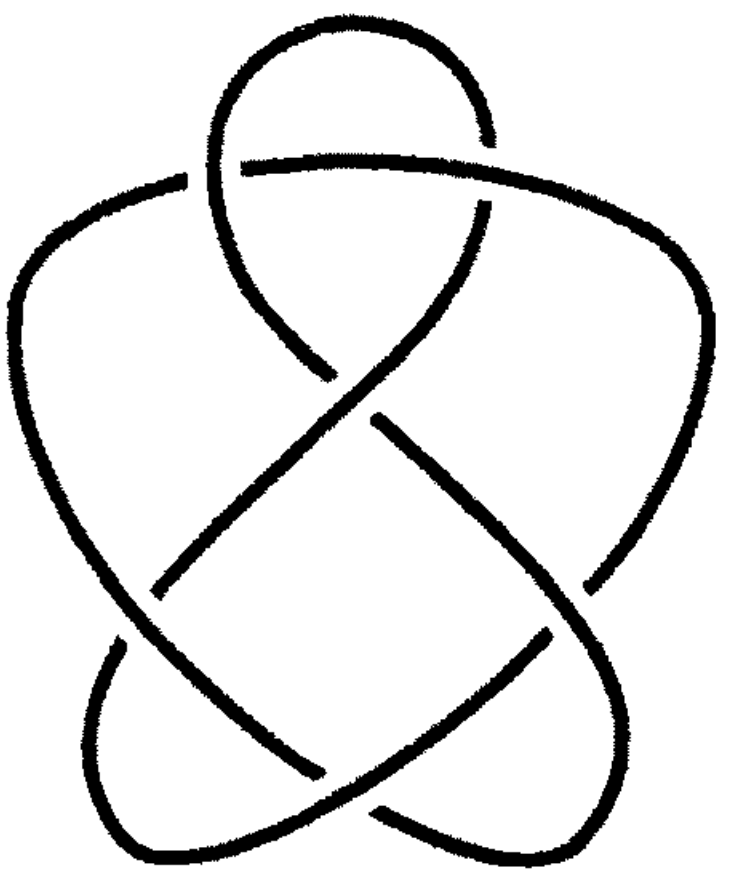
\includegraphics[width=0.8\linewidth]{Blender/ex2-3a.png}
            \caption{$6_2$.}
            \label{fig:ex2-3a}
        \end{subfigure}
        \begin{subfigure}[b]{0.2\linewidth}
            \centering
            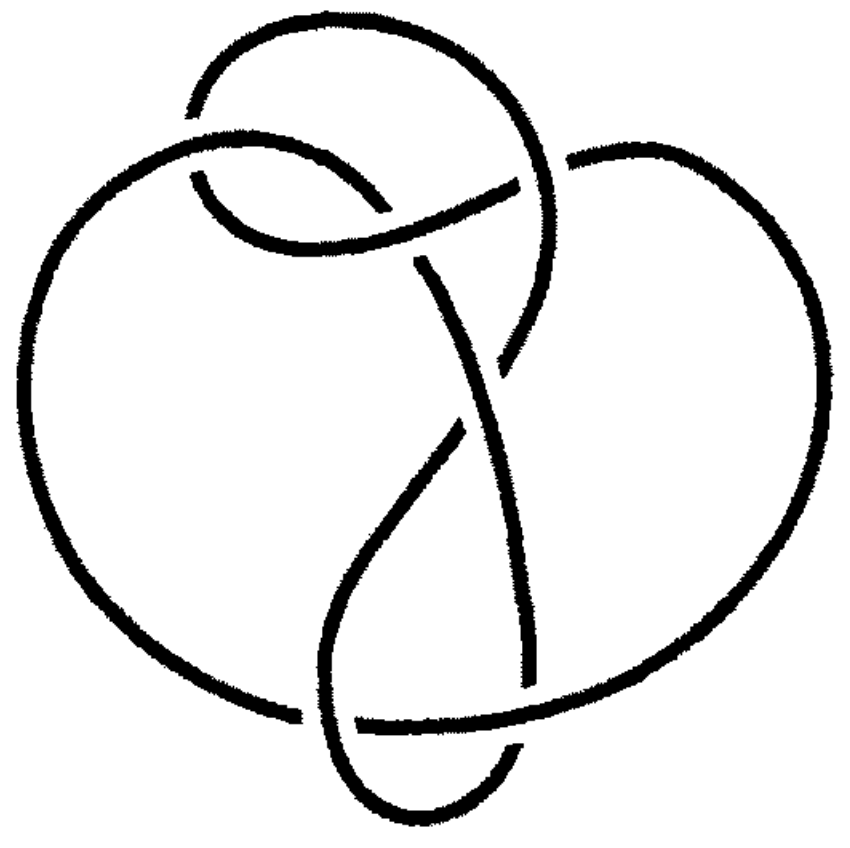
\includegraphics[width=0.7\linewidth]{Blender/ex2-3b.png}
            \caption{$6_3$.}
            \label{fig:ex2-3b}
        \end{subfigure}
        \caption{Knots $6_2$ and $6_3$.}
        \label{fig:ex2-3}
    \end{figure}
    \item Knots can also be reconstructed from Dowker notation. See Figure \ref{fig:reconstruction} for an example of reconstructing an alternating knot from the notation, 8 10 12 2 14 6 4.
    \begin{figure}[h!]
        \centering
        \begin{tikzpicture}[
            every node/.style={black}
        ]
            \begin{knot}[
                clip width=5,
                every strand/.append style={red,thick},
                consider self intersections=true,
                ignore endpoint intersections=false
            ]
                \footnotesize
                \strand[
                    decoration={markings,
                    mark=at position 0.3 with {\arrow{>}},
                    mark=at position 0.9 with {\arrow{>}}},
                    postaction={decorate}
                ] (0,0) to (6,0) to[out=0,in=-90] (7,0.4) to[out=90,in=90,out looseness=0.5] (2,0) node[below left]{2}node[above right]{7} to (2,-0.5);
                \strand (1,0.5) to node[below left]{1}node[above right]{8}  (1,-0.5);
                \strand (3,0.5) to node[below left]{3}node[above right]{10} (3,-0.5);
                \strand (4,0.5) to node[below left]{4}node[above right]{13} (4,-0.5);
                \strand (5,0.5) to node[below left]{5}node[above right]{12} (5,-0.5);
                \strand (6,0.5) to node[below left]{6}node[above right]{11} (6,-0.5);
                \flipcrossings{3,4,6}
                \redraw{1}{(6,0)}
            \end{knot}
        \end{tikzpicture}
        \caption{Constructing a knot projection from its Dowker notation.}
        \label{fig:reconstruction}
    \end{figure}
    \item Our choice in drawing can change the resulting knot.
    \begin{itemize}
        \item 4 6 2 10 12 8 gives two distinct knots.
        \begin{itemize}
            \item \dq{Note that the two knots are composite knots, and that this is refleted in the fact that the sequence 4 6 2 10 12 8 is actually a shuffling of the three numbers 2, 4, 6 and then a shuffling of the three numbers 8, 10, and 12}{38}
        \end{itemize}
        \item When the Dowker notation can be broken into two subpermutations (as above) the knot is composite (unless one subpermutation is trivial).
        \item Any sequence that cannot be split in this way represents either a particular knot or its mirror image.
        \item If the knot is amphicheiral, then the sequence only represent one knot.
    \end{itemize}
    \item A knot and its mirror image are equivalent when projected onto a sphere as opposed to a plane.
    \item \emph{Exercise 2.6}: Draw two projections given by 10 12 2 14 6 4 8, which are inequivalent as projections in the plane but which are equivalent as projections on the sphere.
    \begin{figure}[h!]
        \centering
        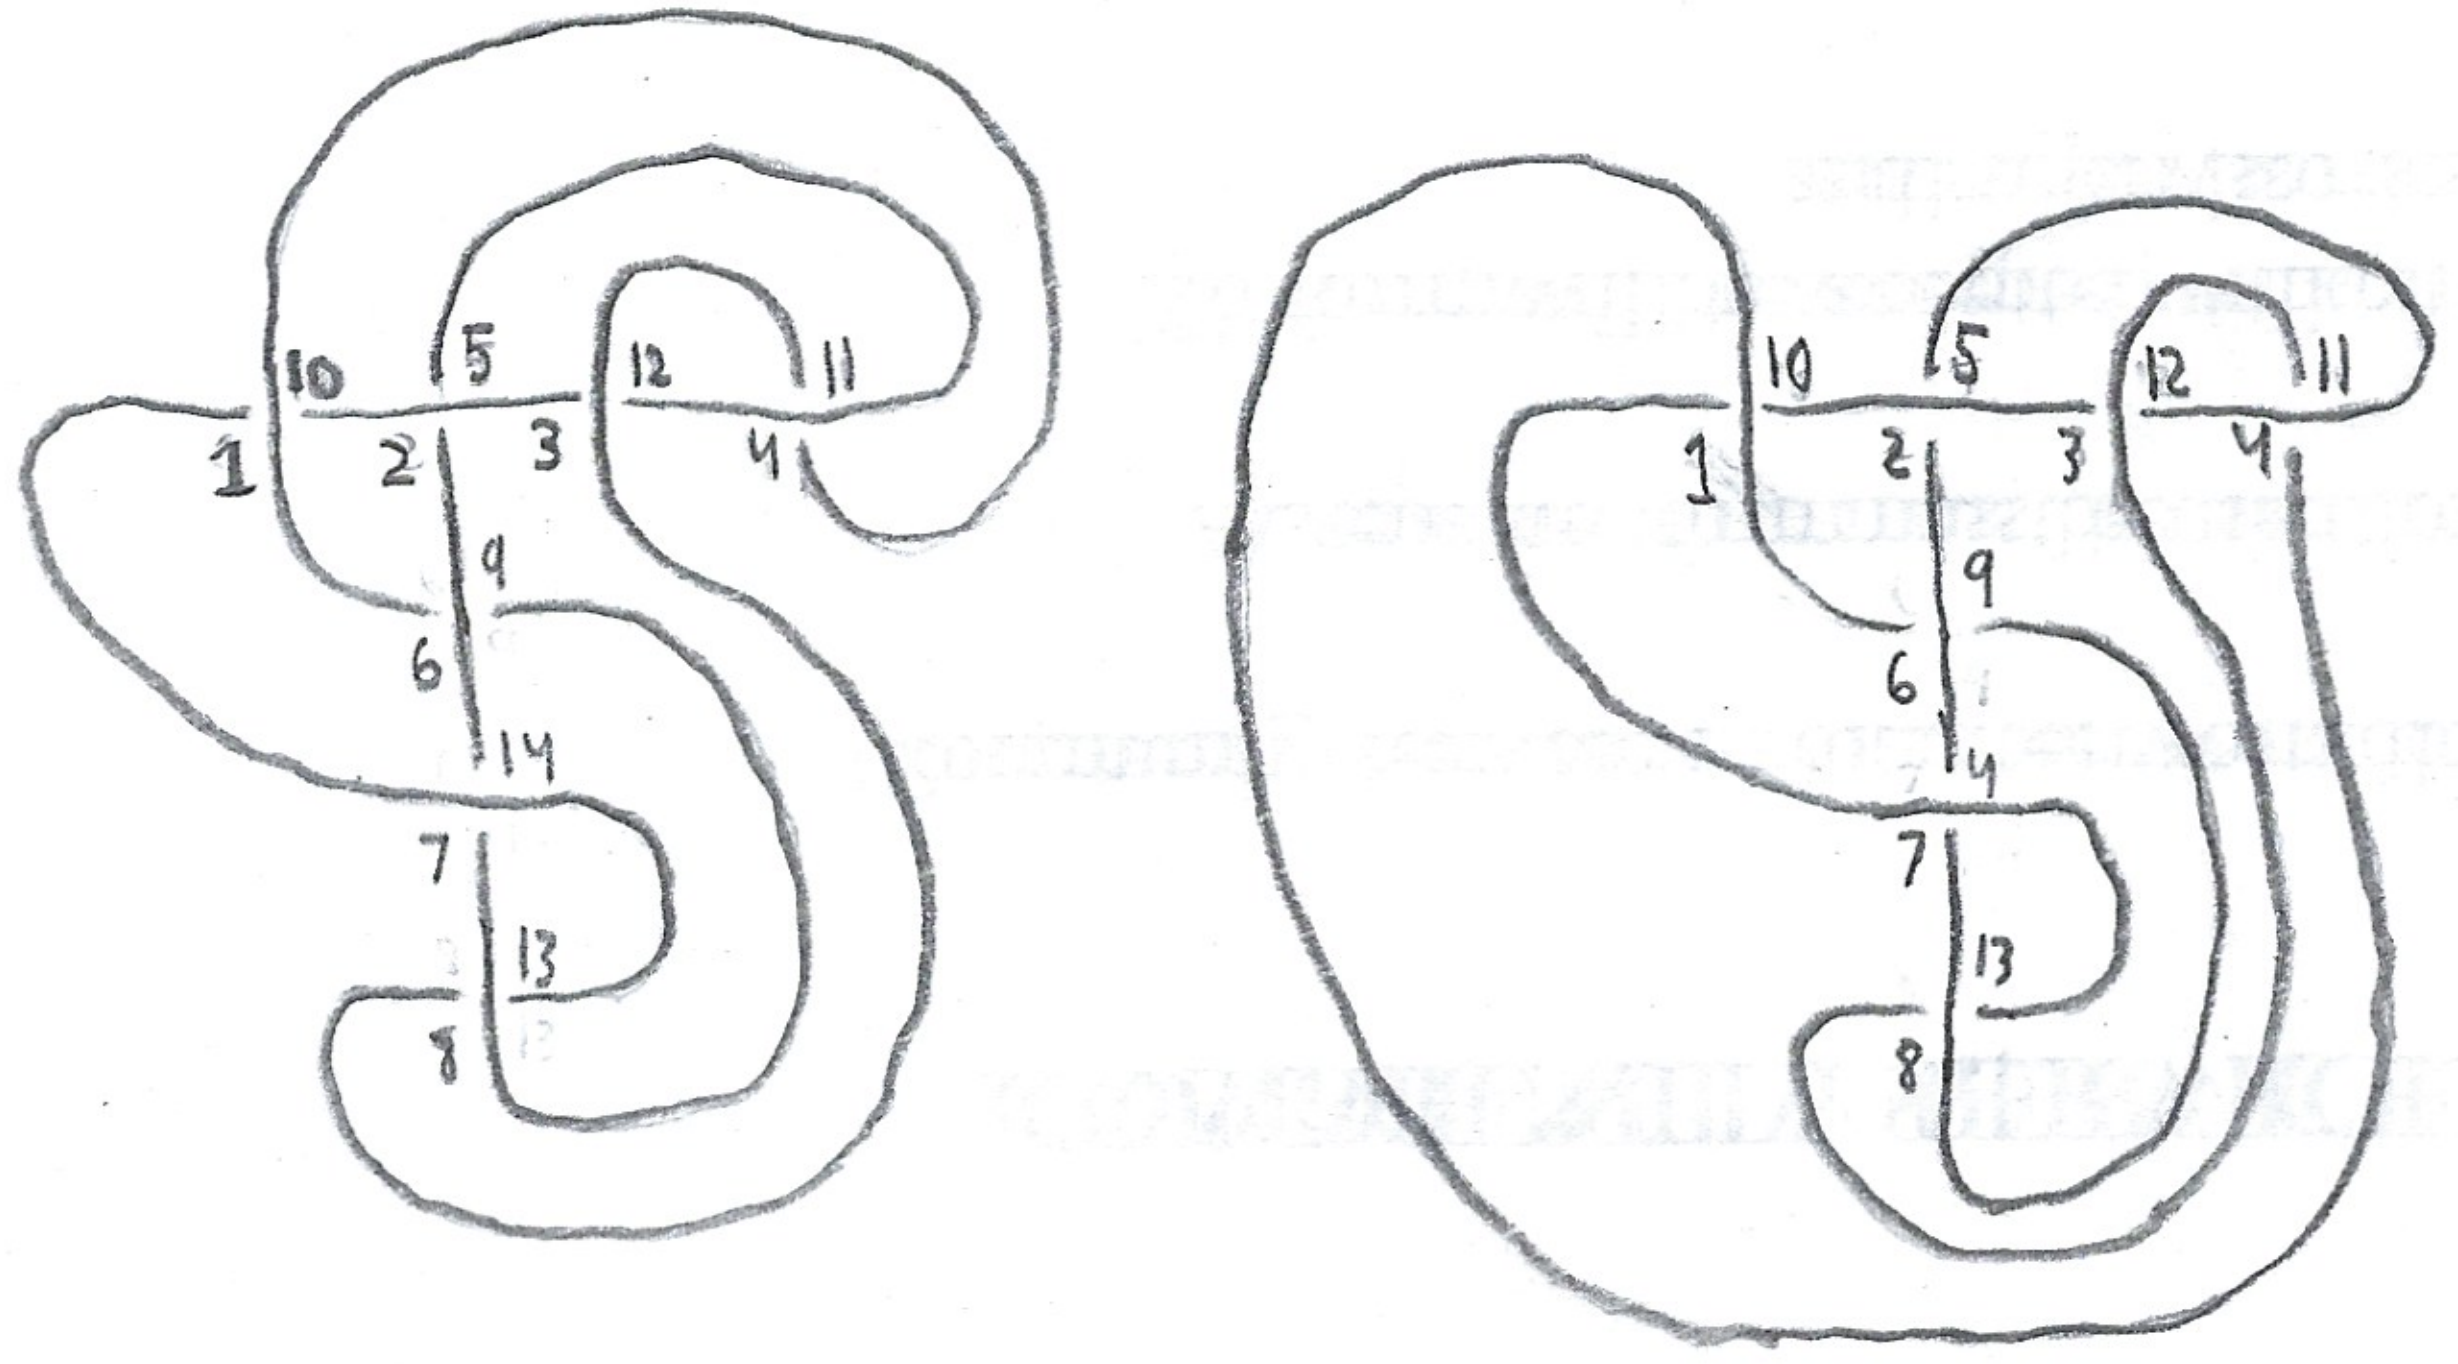
\includegraphics[width=0.5\linewidth]{Blender/ex2-6.png}
        \caption{Solution to \emph{Exercise 2.6}.}
        \label{fig:ex2-6}
    \end{figure}
    \item \emph{Exercise 2.7}: How many different sequences of the integers 2 4 6 8 10 12 14 are there? (This exercise gives us an upper bound on the number of possible alternating knot projections with seven crossings; however, it's far from accurate.)
    \begin{itemize}
        \item There are $7!=5040$ sequences.
    \end{itemize}
    \item There is a slightly modified Dowker notation for nonalternating knots.
    \begin{itemize}
        \item \dq{If the even integer is assigned to the crossing while we are on the overstrand at that crossing, we leave the even integer positive. But if the even integer is assigned to the crossing while we are on the understrand of that crossing, we make the corresponding even numbers negative}{39}
    \end{itemize}
    \item \emph{Exercise 2.9}: How can you recognize from the sequence of numbers that a projection has a trivial crossing in it like in Figure \ref{fig:ex2-9a}? How about recognizing a Type II Reidemeister move that will reduce the number of crossings by two like in Figure \ref{fig:ex2-9b}?
    \begin{figure}[h!]
        \centering
        \begin{subfigure}[b]{0.3\linewidth}
            \centering
            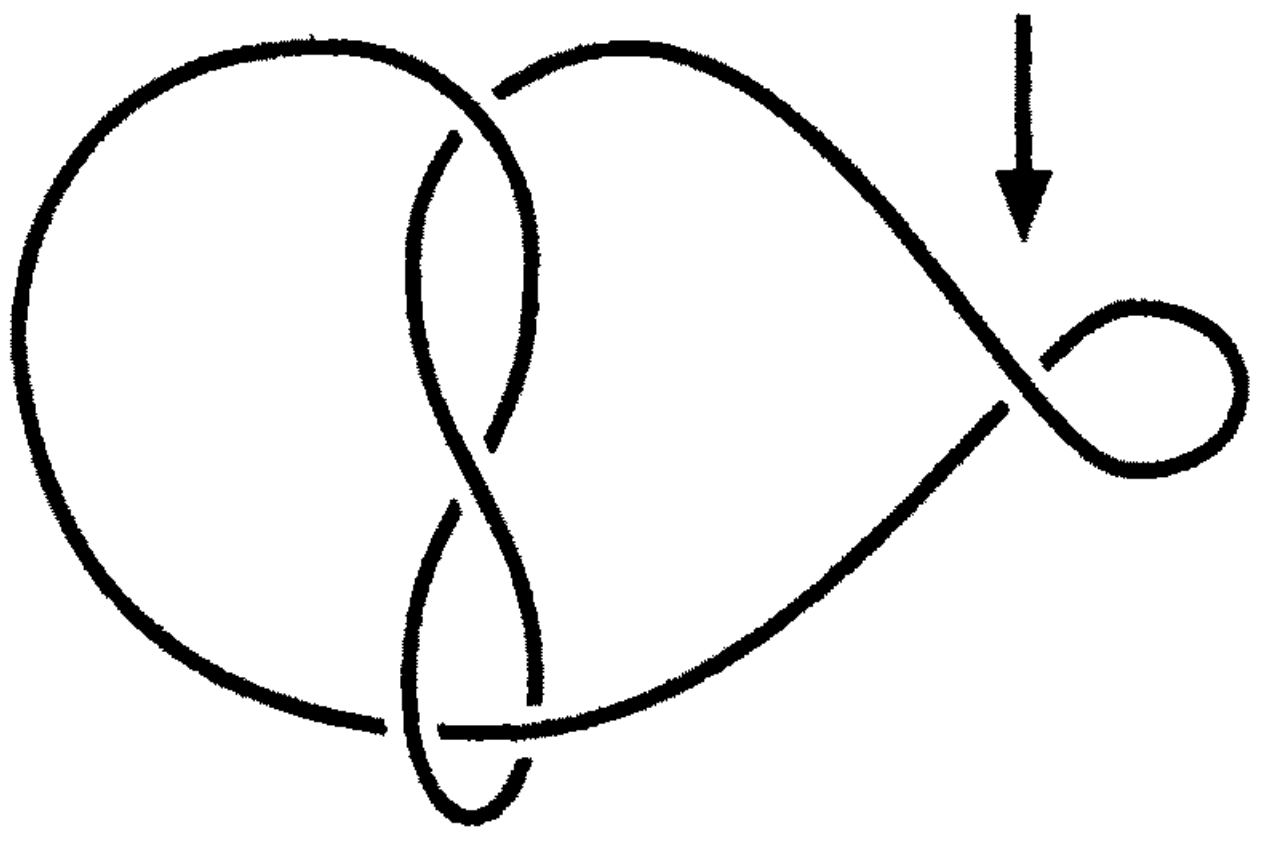
\includegraphics[width=0.6\linewidth]{Blender/ex2-9a.png}
            \caption{Type I Reidemeister move.}
            \label{fig:ex2-9a}
        \end{subfigure}
        \begin{subfigure}[b]{0.3\linewidth}
            \centering
            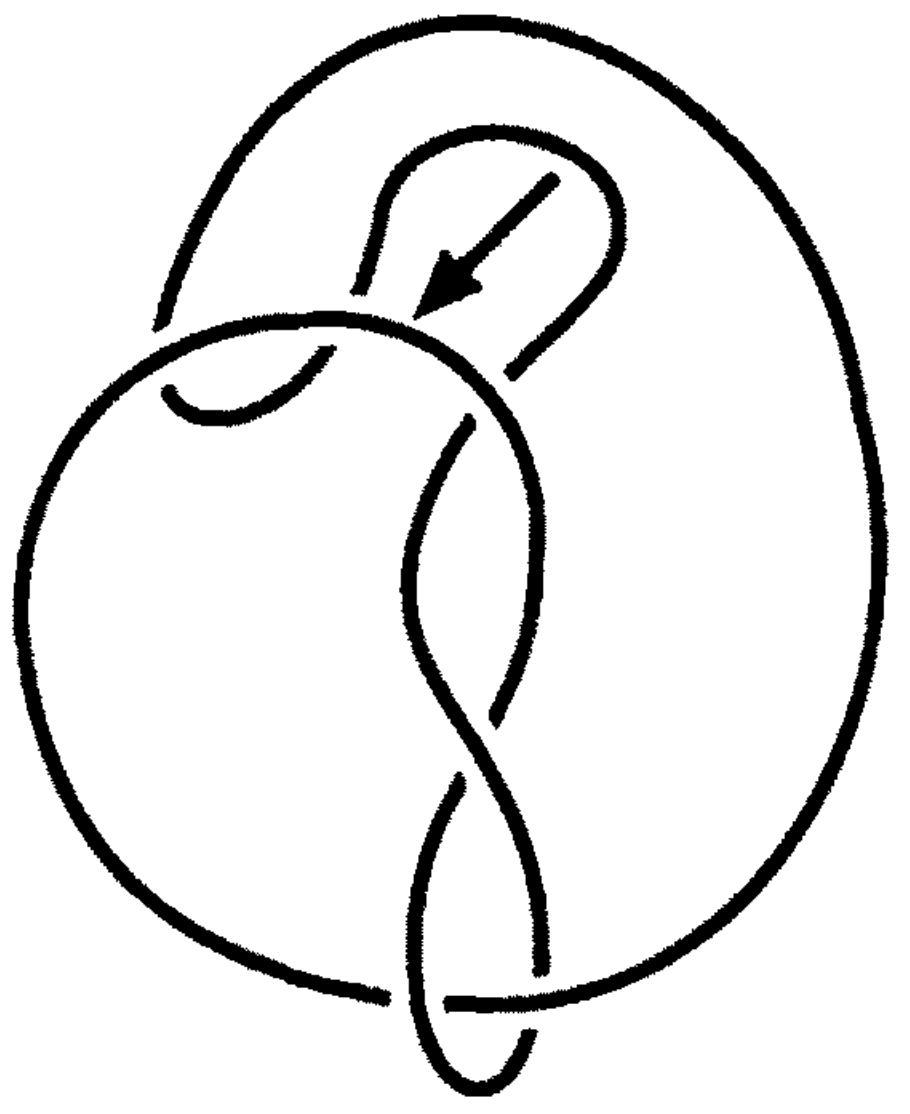
\includegraphics[width=0.53\linewidth]{Blender/ex2-9b.png}
            \caption{Type II Reidemeister move.}
            \label{fig:ex2-9b}
        \end{subfigure}
        \caption{Recognizing extra crossings from the Dowker notation.}
        \label{fig:ex2-9}
    \end{figure}
    \begin{itemize}
        \item A Type I Reidemeister move can be recognized from the Dowker notation sequence by the pairing of two numbers that have an absolute difference of 1. In Figure \ref{fig:ex2-9a}, a sample Dowker notation is 6 2 8 10 4. Since 2 pairs with 3, and $|2-3|=1$, we know that there is a Type I Reidemeister move. Logically, this makes sense because when moving along the orientation, a trivial crossing will be crossed twice in a row.
        \item A Type II Reidemeister move can be recognized from the Dowker notation sequence by a specific characteristic of two pairs: If $(x_1,y_1)$ and $(x_2,y_2)$ is such a pair, where the order is listed such that $|x_2|>|x_1|$ and $|y_1|>|y_2|$, then both of the following must be true.
        \begin{align}
            \big||x_1|-|x_2|\big|=1=\big||y_1|-|y_2|\big| && |x_1-y_2|\neq\big||x_1|-|y_2|\big|\label{eqn:typeIIdowker}
        \end{align}
        In Figure \ref{fig:ex2-9b}, a sample Dowker notation is 8 6 10 $-2$ 12 4. Since ($-2$,7) and (3,6) are pairs that satisfy the above, we know that there is a Type II Reidemeister move. Logically, this makes sense because, when moving along the orientation, such crossings' numbers will be sequential both times crossed (confirmed by the left statement in Equation \ref{eqn:typeIIdowker}). Additionally, the even numbers must have opposite signs or the strand would be linked, as opposed to entirely above or below (confirmed by the right statement in Equation \ref{eqn:typeIIdowker}).
    \end{itemize}
    \item The most consequential fact of Dowker notation is that it allows us to \dq{feed projections of knots into the computer simply as a sequence of numbers}{40}
\end{itemize}


\subsection{Conway's Notation}\label{sss:Conway}
\begin{itemize}
    \item Particularly suited to calculations involving \textbf{tangles}.
    \item \textbf{Tangle}: \dq{A region [in a knot or link] in the projection plane surrounded by a circle such that the knot or link crosses the circle exactly four times}{41}
    \begin{itemize}
        \item These four crossings will be thought of as occurring in the four ordinal compass directions.
    \end{itemize}
    \item Tangles can be thought of as building blocks in knot or link projections.
    \item \textbf{Equivalent}: Two tangle projections that can be transformed into each other via a series of Reidemeister moves \dq{while the four endpoints of the strings in the tangle remain fixed and while the strings of the tangle never journey outside the circle defining the tangle}{41}
    \item Notice that, if a knot is formed by gluing together the tangle's ends in pairs, the knot is equivalent to other projections of itself as long as the tangles are equivalent (by a series of Reidemeister moves).
    \item Tangles, such as the one in Figure \ref{fig:tanglesc} are denoted by the number of left-hand twists (crossings).
    \begin{itemize}
        \item If we had twisted the tangle the other way, we would have called it $-3$.
        \item More simply, \dq{for a positive-integer twist, the overstrand always has a positive slope, if we think of it as a small segment of a line [perhaps a cubic, in the case of Figure \ref{fig:tanglesc}]}{42}
    \end{itemize}
    \begin{figure}[h!]
        \centering
        \begin{subfigure}[b]{0.3\linewidth}
            \centering
            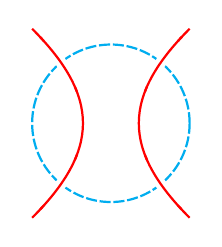
\begin{tikzpicture}
                \begin{knot}[
                    clip width=5
                ]
                    \strand[cyan,thick,only when rendering/.style={dashed,dash pattern={on 4pt off 1pt}}] circle (1cm);
                    \strand[red,thick] (-1,1.2) to[out=-45,in=45,looseness=1.3] (-1,-1.2);
                    \strand[red,thick] (1,1.2) to[out=-135,in=135,looseness=1.3] (1,-1.2);
                    \flipcrossings{1,2,3,4}
                \end{knot}
            \end{tikzpicture}
            \caption{The $\infty$ tangle.}
            \label{fig:tanglesa}
        \end{subfigure}
        \begin{subfigure}[b]{0.3\linewidth}
            \centering
            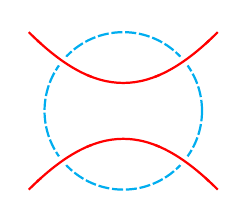
\begin{tikzpicture}
                \begin{knot}[
                    clip width=5
                ]
                    \strand[cyan,thick,only when rendering/.style={dashed,dash pattern={on 4pt off 1pt}}] circle (1cm);
                    \strand[red,thick] (-1.2,1) to[out=-45,in=-135,looseness=1.3] (1.2,1);
                    \strand[red,thick] (-1.2,-1) to[out=45,in=135,looseness=1.3] (1.2,-1);
                    \flipcrossings{1,2,3,4}
                \end{knot}
            \end{tikzpicture}
            \caption{The $0$ tangle.}
            \label{fig:tanglesb}
        \end{subfigure}
        \begin{subfigure}[b]{0.3\linewidth}
            \centering
            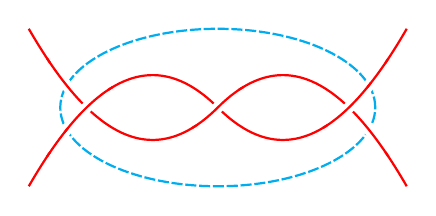
\begin{tikzpicture}
                \begin{knot}[
                    clip width=5,
                    ignore endpoint intersections=false
                ]
                    \strand[cyan,thick,only when rendering/.style={dashed,dash pattern={on 4pt off 1pt}}] ellipse (2cm and 1cm);
                    \strand[red,thick] (-2.4,-1)
                        to[out=60,in=135,looseness=1.3] (0,0)
                        to[out=-45,in=-120,looseness=1.3] (2.4,1)
                    ;
                    \strand[red,thick] (-2.4,1)
                        to[out=-60,in=-135,looseness=1.3] (0,0)
                        to[out=45,in=120,looseness=1.3] (2.4,-1)
                    ;
                    \flipcrossings{1,2,3,4,6}
                \end{knot}
            \end{tikzpicture}
            \caption{The $3$ tangle.}
            \label{fig:tanglesc}
        \end{subfigure}
        \caption{Tangles.}
        \label{fig:tangles}
    \end{figure}
    \item \textbf{0 tangle}: The simplest of all tangles (by definition). \emph{Also known as} \textbf{trivial tangle}. See Figure \ref{fig:tanglesb}.
    \item If we reflect the 3 tangle across a line connecting the NW and SE corners, and then proceed to extrude the NE and SE strands, twisting positively twice, we yield the tangle, 3 2.
    \item If we reflect 3 2 across the same line, and then proceed to extrude the NE and SE stands, twisting negatively four times, we yield the tangle, 3 2 $-4$.
    \item \textbf{Rational tangle}: Any tangle that can be constructed in the manner described in the above 2 bullet points.
    \begin{itemize}
        \item Note that if the tangle is represented by an even number of integers, it can be thought of as being constructed from the $\infty$ tangle, and vice versa for the 0 tangle.
    \end{itemize}
    \item \emph{Exercise 2.10}: Draw the rational tangles corresponding to 2 $-3$ 4 5 and 3 $-1$ 3 $-3$ 2.
    \begin{figure}[H]
        \centering
        \begin{subfigure}[b]{0.4\linewidth}
            \centering
            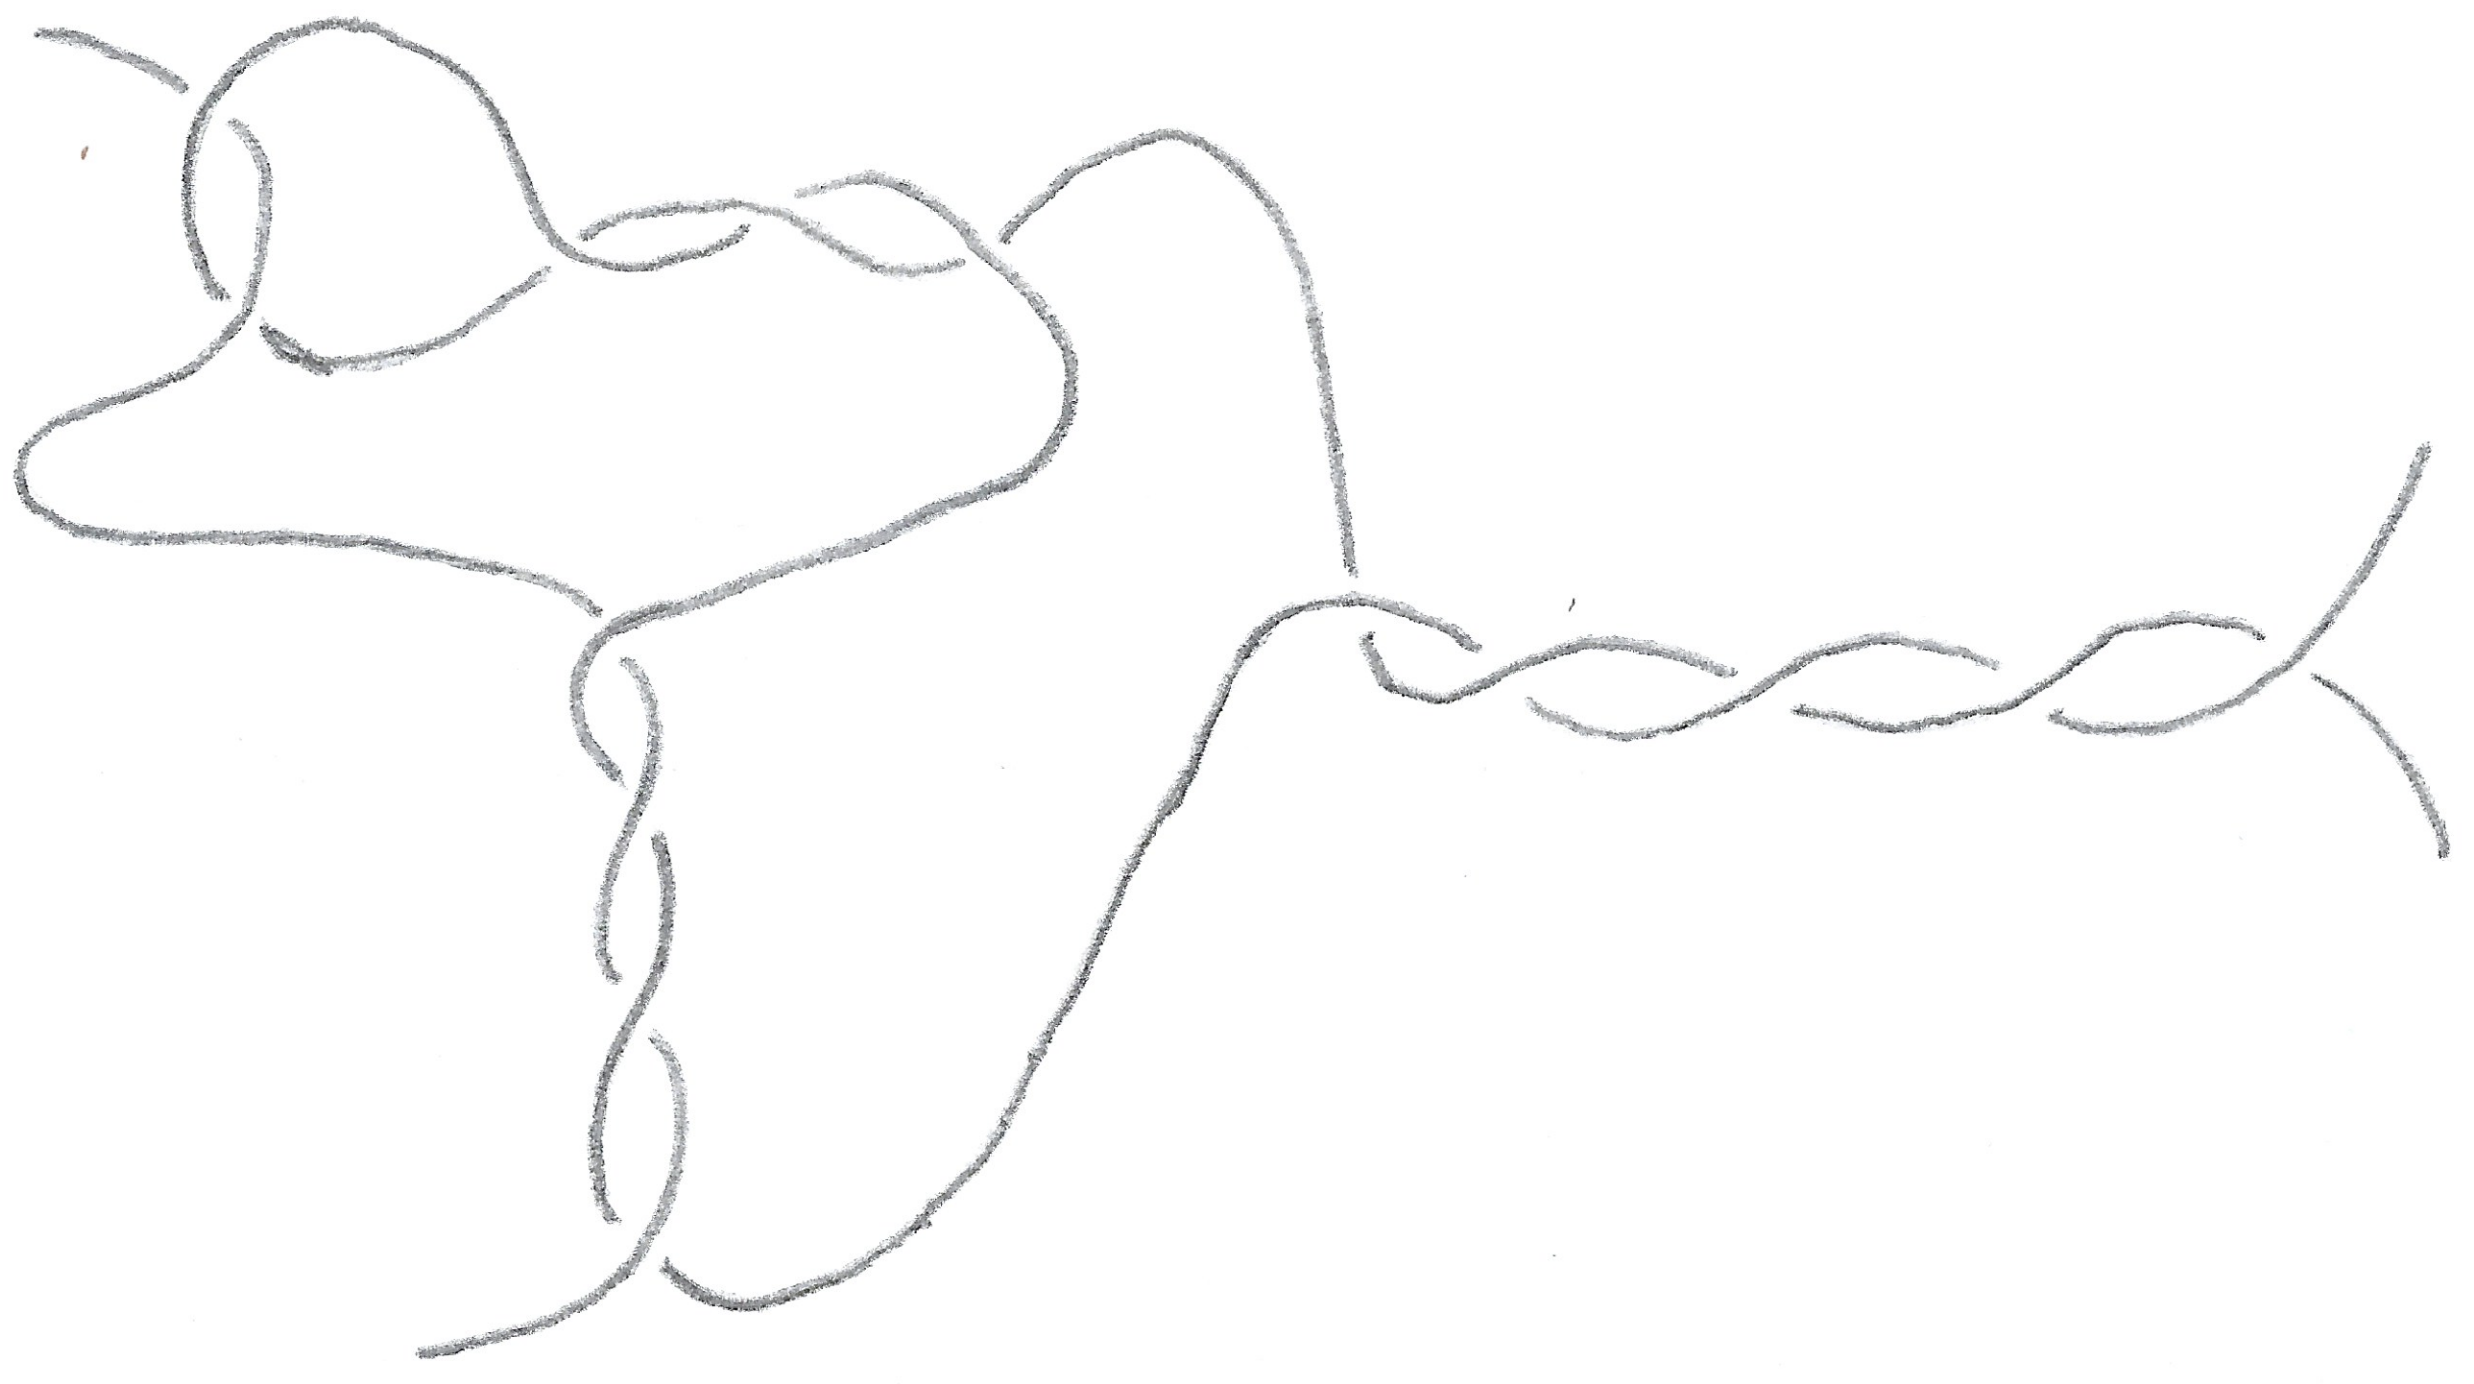
\includegraphics[width=\linewidth]{Blender/ex2-10a.png}
            \caption{The tangle, 2 $-3$ 4 5.}
            \label{fig:ex2-10a}
        \end{subfigure}
        \begin{subfigure}[b]{0.4\linewidth}
            \centering
            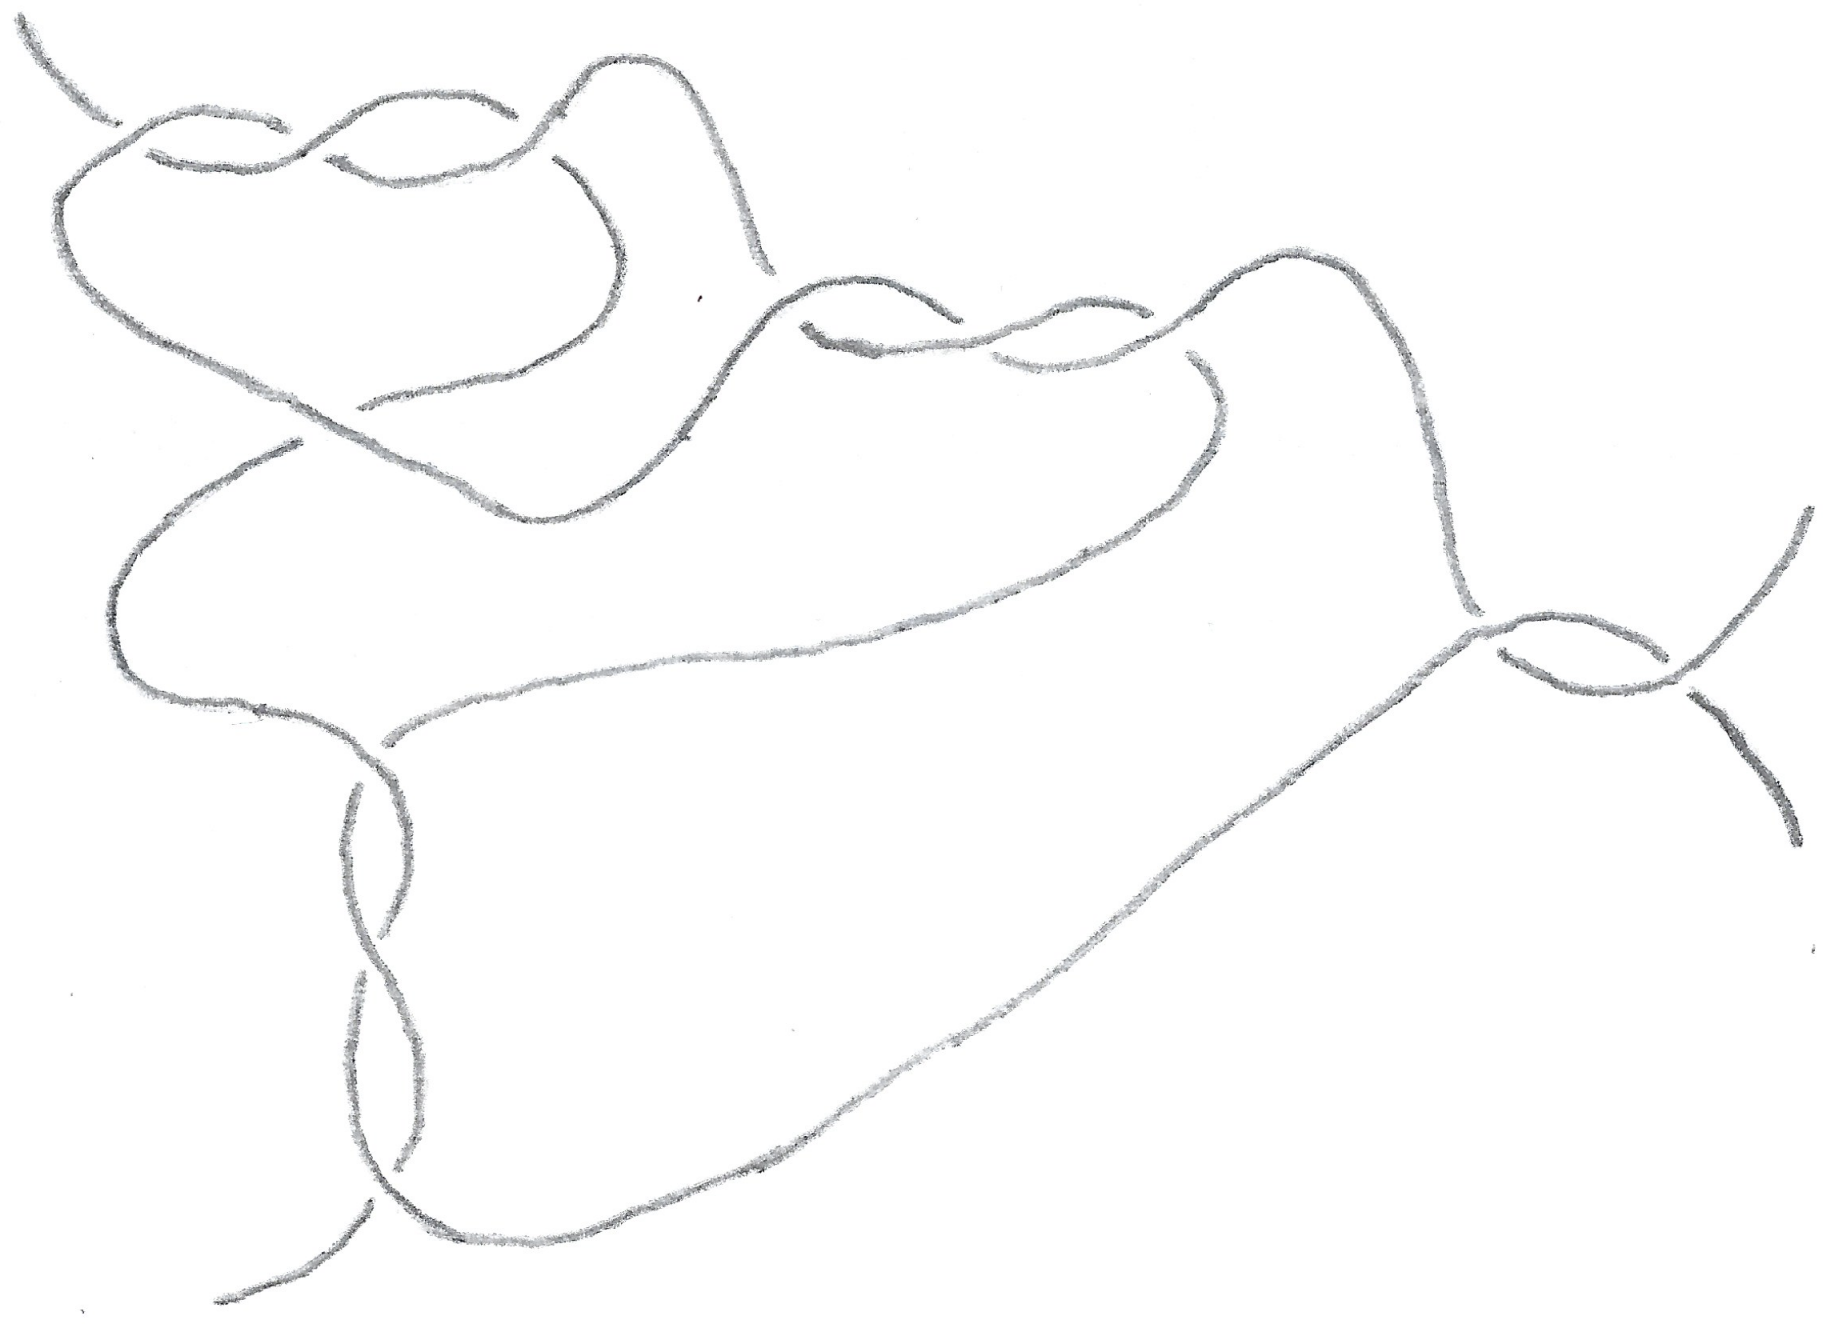
\includegraphics[width=0.8\linewidth]{Blender/ex2-10b.png}
            \caption{The tangle, 3 $-1$ 3 $-3$ 2.}
            \label{fig:ex2-10b}
        \end{subfigure}
        \caption{Solution to \emph{Exercise 2.10}}
        \label{fig:ex2-10}
    \end{figure}
    \item There is an extremely simple way to tell if two rational tangles are equivalent from their notation: \textbf{continued fractions}.
    \item \textbf{Continued fraction}: A fraction obtained through the iterative process of summing a number and its reciprocal.
    \begin{itemize}
        \item For example, given the three numbers a, b, and c, the continued fraction would be the following.
        \begin{equation}
            c+\frac{1}{b+\frac{1}{a}}
        \end{equation}
    \end{itemize}
    \begin{figure}[H]
        \centering
        \begin{subfigure}[b]{0.3\linewidth}
            \centering
            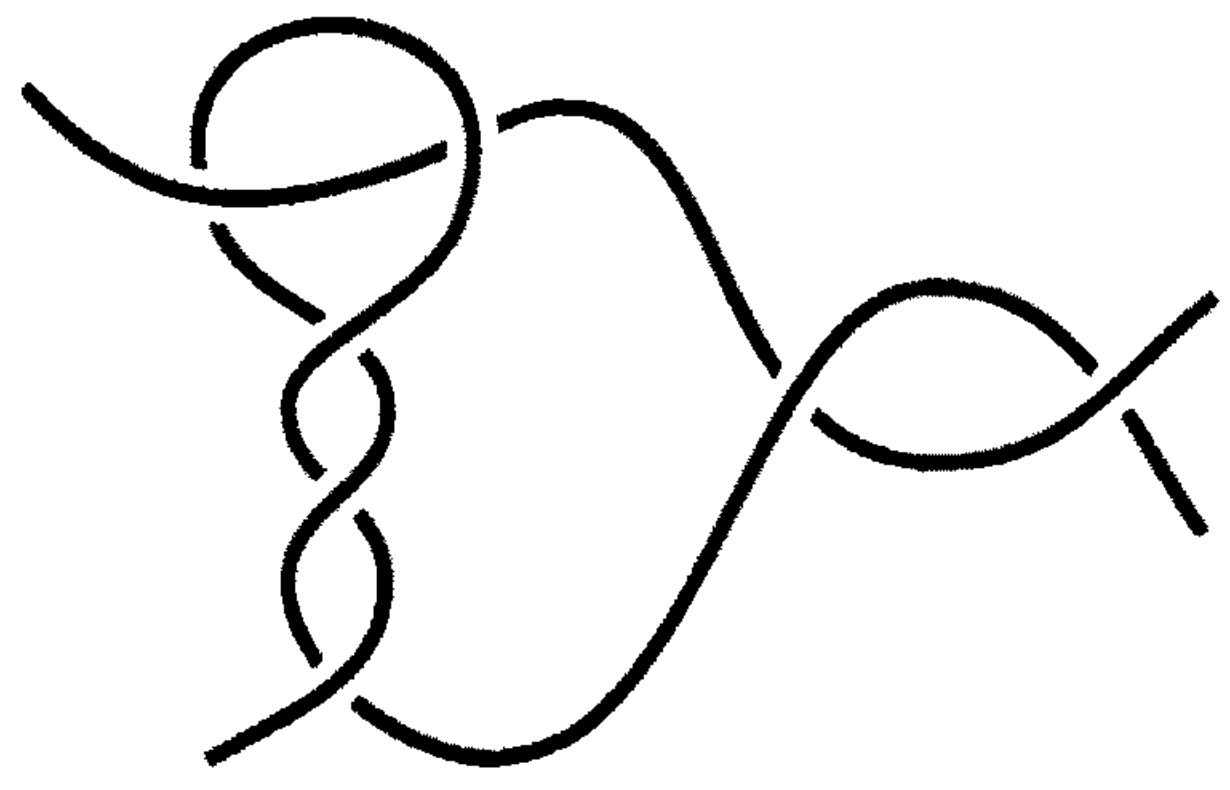
\includegraphics[width=0.56\linewidth]{Blender/ex2-12a.png}
            \caption{The tangle, $-2$ 3 2.}
            \label{fig:ex2-12a}
        \end{subfigure}
        \begin{subfigure}[b]{0.3\linewidth}
            \centering
            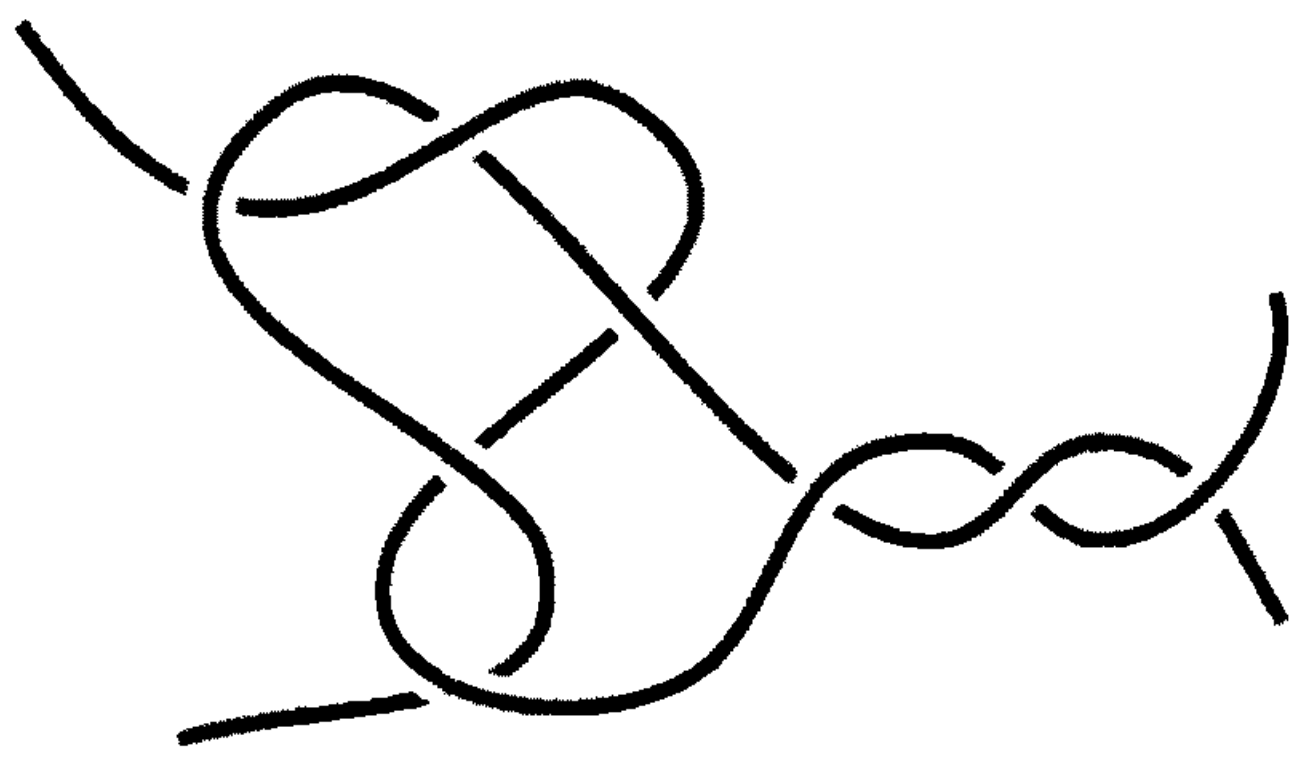
\includegraphics[width=0.56\linewidth]{Blender/ex2-12b.png}
            \caption{The tangle, 3 $-2$ 3.}
            \label{fig:ex2-12b}
        \end{subfigure}
        \caption{Two equivalent tangles.}
        \label{fig:ex2-12}
    \end{figure}
    \item Applied to knot theory, we know that the tangles, $-2$ 3 2 and 3 $-2$ 3, (seen in Figure \ref{fig:ex2-12}) are equivalent because of the following.
    \begin{align}
        \begin{split}
            2+\frac{1}{3+\frac{1}{-2}} &= 3+\frac{1}{-2+\frac{1}{3}}\\
            2+\frac{1}{\frac{5}{2}} &= 3+\frac{1}{\frac{-5}{3}}\\
            2+\frac{2}{5} &= 3+\frac{-3}{5}\\
            \frac{12}{5} &= \frac{12}{5}\\
        \end{split}
    \end{align}
    \item \emph{Exercise 2.13}: Determine which of the four rational tangles in Figure \ref{fig:ex2-13} are equivalent$^[$\footnote{Idea for first paper: Prove that a series of NE$\leftrightarrow$SE and SE$\leftrightarrow$SW moves is sufficient to generate any rational tangle (like Reidemeister moves). Apply these findings to defining a tangle from a projection. Potentially create a new notation (show how this notation and the current tangle notation convert).}$^]$.
    \begin{figure}[h!]
        \centering
        \begin{subfigure}[b]{0.2\linewidth}
            \centering
            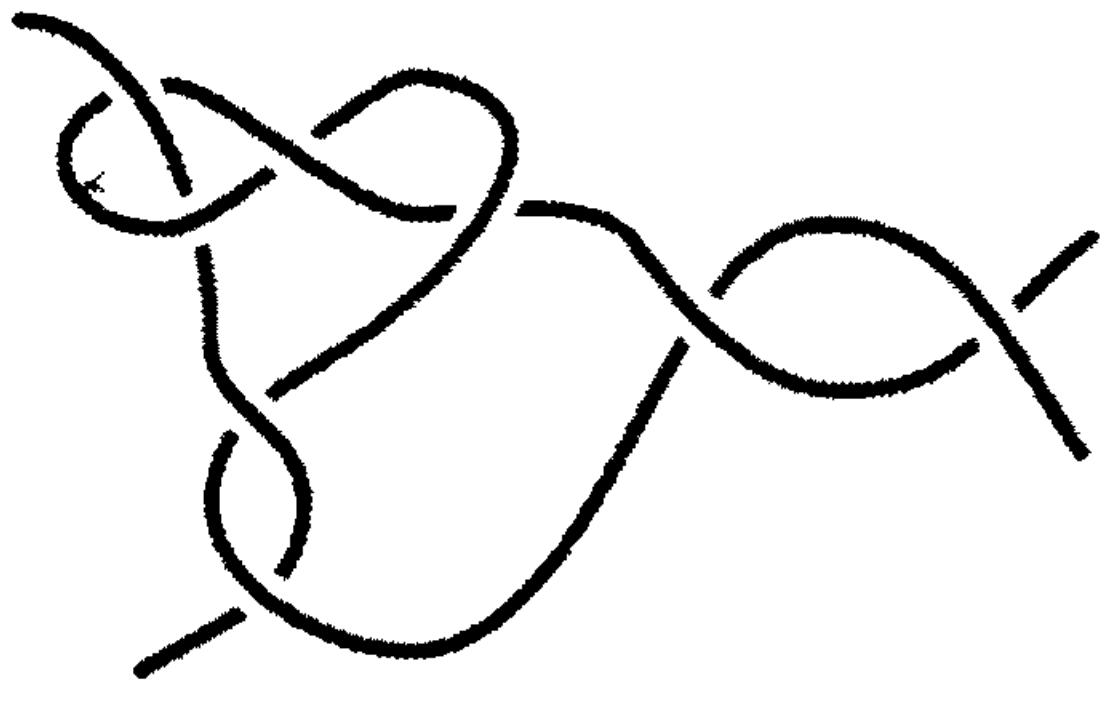
\includegraphics[width=0.8\linewidth]{Blender/ex2-13a.png}
            \caption{Tangle 1.}
            \label{fig:ex2-13a}
        \end{subfigure}
        \begin{subfigure}[b]{0.2\linewidth}
            \centering
            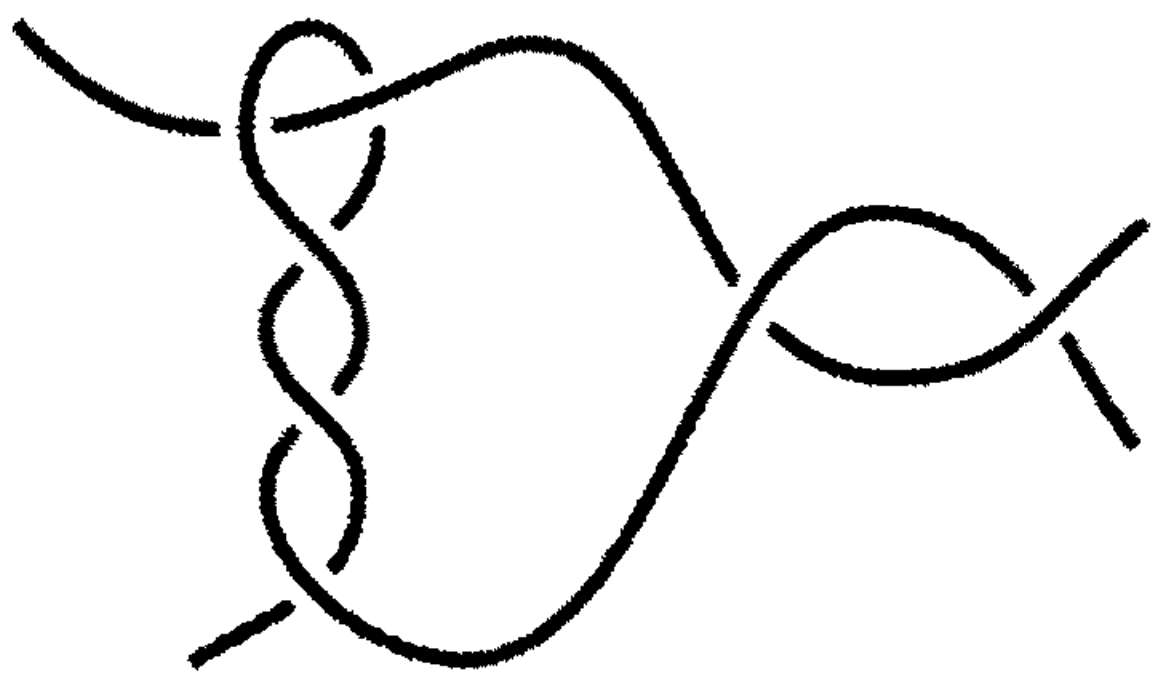
\includegraphics[width=0.8\linewidth]{Blender/ex2-13b.png}
            \caption{Tangle 2.}
            \label{fig:ex2-13b}
        \end{subfigure}
        \begin{subfigure}[b]{0.25\linewidth}
            \centering
            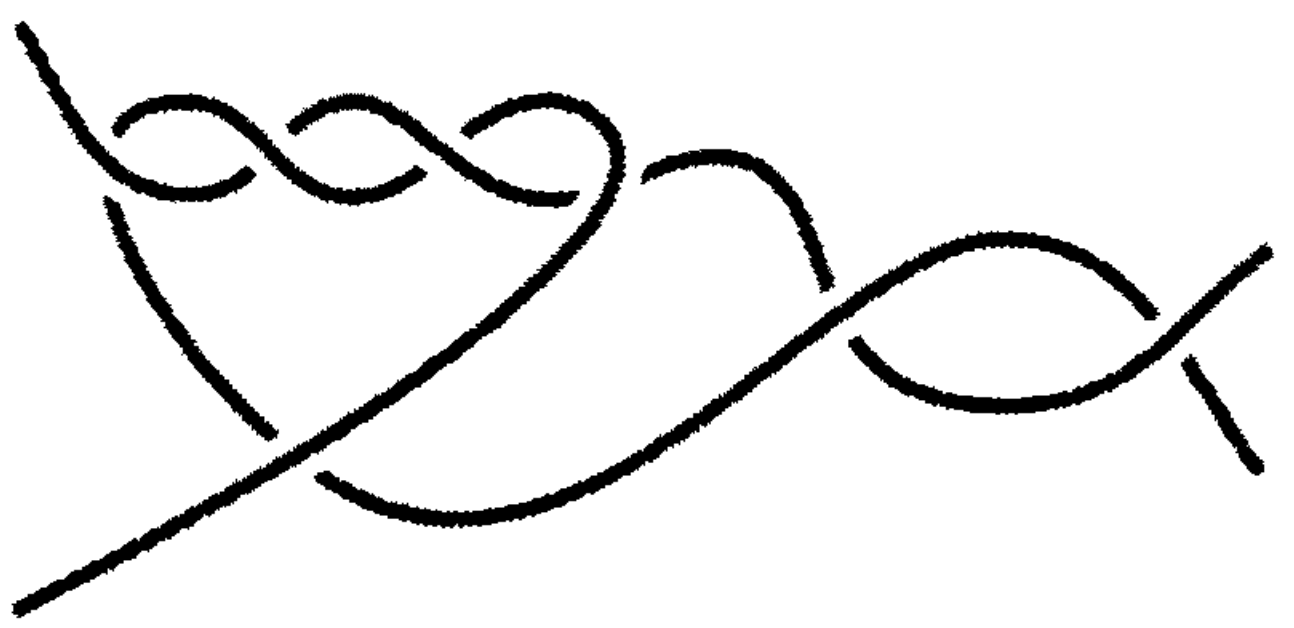
\includegraphics[width=0.8\linewidth]{Blender/ex2-13c.png}
            \caption{Tangle 3.}
            \label{fig:ex2-13c}
        \end{subfigure}
        \begin{subfigure}[b]{0.16\linewidth}
            \centering
            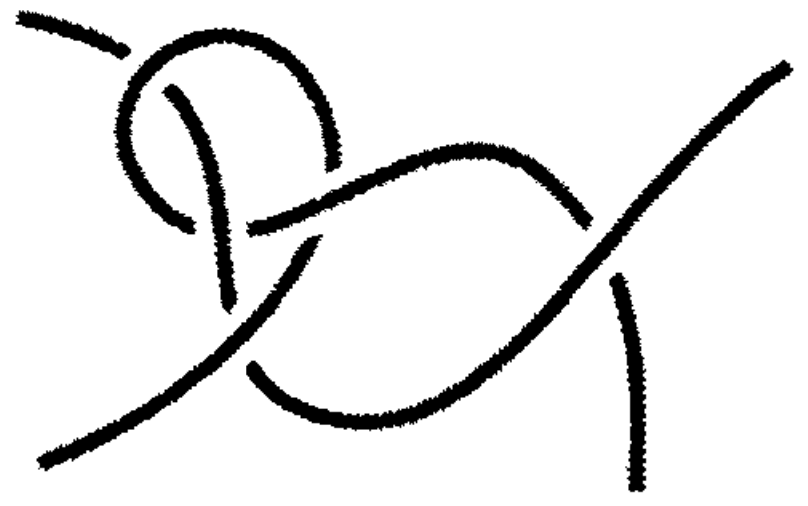
\includegraphics[width=0.8\linewidth]{Blender/ex2-13d.png}
            \caption{Tangle 4.}
            \label{fig:ex2-13d}
        \end{subfigure}
        \caption{Four rational tangles.}
        \label{fig:ex2-13}
    \end{figure}
    \begin{itemize}
        \item Tangle 1 (Figure \ref{fig:ex2-13a}) can be denoted $-1$ $-1$ $-2$ $-2$ $-2$.
        \begin{itemize}
            \item Its continued fraction simplifies as follows.
            \begin{align}
                \begin{split}
                    -2+\frac{1}{-2+\frac{1}{-2+\frac{1}{-1+\frac{1}{-1}}}} &= -2+\frac{1}{-2+\frac{1}{-2+\frac{1}{-2}}}\\
                    &= -2+\frac{1}{-2+\frac{-2}{5}}\\
                    &= -2+\frac{-5}{12}\\
                    &= \frac{-29}{12}\\
                \end{split}
            \end{align}
        \end{itemize}
        \item Tangle 2 (Figure \ref{fig:ex2-13b}) can be denoted 2 $-3$ 2.
        \begin{itemize}
            \item Its continued fraction simplifies as follows.
            \begin{align}
                \begin{split}\label{eqn:ex2-13b}
                    2+\frac{1}{-3+\frac{1}{2}} &= 2+\frac{-2}{5}\\
                    &= \frac{8}{5}\\
                \end{split}
            \end{align}
        \end{itemize}
        \item Tangle 3 (Figure \ref{fig:ex2-13c}) can be denoted $-4$ 1 2.
        \begin{itemize}
            \item Its continued fraction simplifies as follows.
            \begin{align}
                \begin{split}
                    2+\frac{1}{1+\frac{1}{-4}} &= 2+\frac{4}{3}\\
                    &= \frac{10}{3}\\
                \end{split}
            \end{align}
        \end{itemize}
        \item Tangle 4 (Figure \ref{fig:ex2-13d}) can be denoted 1 1 1 1 1.
        \begin{itemize}
            \item Its continued fraction simplifies as follows.
            \begin{align}
                \begin{split}\label{eqn:ex2-13d}
                    1+\frac{1}{1+\frac{1}{1+\frac{1}{1+\frac{1}{1}}}} &= 1+\frac{1}{1+\frac{1}{1+\frac{1}{2}}}\\
                    &= 1+\frac{1}{1+\frac{2}{3}}\\
                    &= 1+\frac{3}{5}\\
                    &= \frac{8}{5}\\
                \end{split}
            \end{align}
        \end{itemize}
        \item Therefore, tangles 2 and 4 (Figures \ref{fig:ex2-13b} and \ref{fig:ex2-13d}, respectively) are equivalent by equations \ref{eqn:ex2-13b} and \ref{eqn:ex2-13d}.
    \end{itemize}
    \item If we close off the ends of a rational tangle, i.e. NE to NW and SE to SW, we form a rational link.
    \item If the link is a knot, we can denote it by its tangle. For example, the figure-eight knot is a rational knot with \textbf{Conway notation} 22 (because of the two twists twice in its center and the gluing of its ends).
    \item \textbf{Conway's notation}: A method of denoting knots by their tangles (all aforementioned theory in this section).
    \item Multiplying tangles:
    \begin{itemize}
        \item Reflect the left tangle across its NW to SE diagonal and then glue its new NE and SE ends to the NW and SW ends, respectively, of the adjacent (to the right) tangle.
        \item Multiplying a rational tangle by an integer tangle will always generate a rational tangle, e.g. 32 comes from multiplying 3 by 2.
        \item To reflect a tangle over its NW-SE line, multiply it by the tangle, 0.
    \end{itemize}
    \begin{figure}[h!]
        \centering
        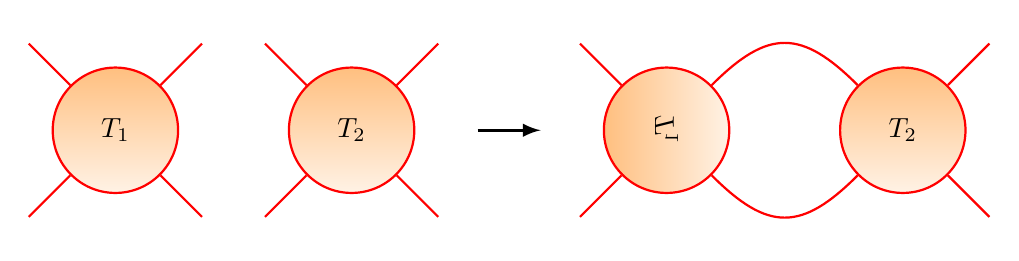
\begin{tikzpicture}
            \node (a) [draw=red,circle,thick,inner sep=4mm] [top color=orange!50,bottom color=orange!10] [xshift=-5cm]                     {$T_1$}
                edge [red,thick] +([xshift=-5cm]1.1,1.1)
                edge [red,thick] +([xshift=-5cm]-1.1,1.1)
                edge [red,thick] +([xshift=-5cm]1.1,-1.1)
                edge [red,thick] +([xshift=-5cm]-1.1,-1.1)
            ;
            \node (b) [draw=red,circle,thick,inner sep=4mm] [top color=orange!50,bottom color=orange!10] [xshift=-2cm]                     {$T_2$}
                edge [red,thick] +([xshift=-2cm]1.1,1.1)
                edge [red,thick] +([xshift=-2cm]-1.1,1.1)
                edge [red,thick] +([xshift=-2cm]1.1,-1.1)
                edge [red,thick] +([xshift=-2cm]-1.1,-1.1)
            ;
            \node (c) [draw=red,circle,thick,inner sep=4mm] [left color=orange!50,right color=orange!10] [rotate=90,xscale=-1,yshift=-2cm] {$T_1$}
                edge [red,thick] +([xshift=2cm]-1.1,1.1)
                edge [red,thick] +([xshift=2cm]-1.1,-1.1)
            ;
            \node (d) [draw=red,circle,thick,inner sep=4mm] [top color=orange!50,bottom color=orange!10] [xshift=5cm]                     {$T_2$}
                edge [red,thick] +([xshift=5cm]1.1,1.1)
                edge [red,thick] +([xshift=5cm]1.1,-1.1)
                edge [red,thick,bend left=45,looseness=1.4]  (c)
                edge [red,thick,bend left=-45,looseness=1.4] (c)
            ;
    
            \draw[very thick,-latex] (-0.4,0) -- (0.4,0);
        \end{tikzpicture}
        \caption{Multiplying tangles.}
        \label{fig:tanglemultiply}
    \end{figure}
    \item Adding tangles:
    \begin{itemize}
        \item Glue the left tangle's NE and SE ends to the right tangle's NW and SW ends, respectively.
        \item Note that no reflecting occurs here.
        \item \dq{If we multiply each tangle in a sequence of tangles by 0, and then add them all together, we denote the resultant tangle by the sequence of numbers that stand for the original tangles, only now separated by commas}{48}
    \end{itemize}
    \item \textbf{Pretzel knot}: \dq{A knot obtained from a tangle represented by a finite number of integers separated by commas}{48}
    \item \textbf{Algebraic tangle}: \dq{Any tangle obtained by the operations of addition and multiplication on rational tangles}{48}
    \item \textbf{Algebraic link}: \dq{A link formed when we connect the NW string to the NE string and the SW string to the SE string on an algebraic tangle}{48} \emph{Also known as} \textbf{aborescent link}.
    \begin{itemize}
        \item Denoted the same way as a tangle.
        \item Fun fact: The trefoil knot (Figure \ref{fig:circletrefoilb}) is an algebraic link of the 3 tangle (Figure \ref{fig:tanglesc}).
    \end{itemize}
    \item \textbf{Additive identity}: A quantity that can be added to a second quantity without changing that second quantity.
    \begin{itemize}
        \item 0 is an additive identity for the real numbers.
    \end{itemize}
    \item \emph{Exercise 2.21}: Is there an additive identity for tangles?
    \begin{itemize}
        \item The 0 tangle (Figure \ref{fig:tanglesb}) is an additive identity for tangles. Adding the 0 tangle does the same thing as extruding (performing a planar isotropy on) the NE and SE strands. Such an addition does not change the relative position of any strand's ordinal end(s).
        \item Continuing the analogy to the real numbers, it makes sense that the 0 tangle would be analogous to 0, the real number.
    \end{itemize}
    \item \textbf{Multiplicative identity}: A quantity that can be multiplied by a second quantity without changing that second quantity.
    \begin{itemize}
        \item 1 is a multiplicative identity for the real numbers.
    \end{itemize}
    \item \emph{Exercise 2.22}: Is there a multiplicative identity for tangles? Is it the same if you multiply a tangle by it on the right side or the left side?
    \begin{itemize}
        \item The 0 tangle (Figure \ref{fig:tanglesb}) is a multiplicative identity for tangles. Multiplying the 0 tangle does the same thing as extruding (performing a planar isotropy on) the SE and SW strands. Such a multiplication does not change the relative position of any strand's ordinal end(s).
        \item To part 2, yes.
    \end{itemize}
    \item The analogy to real numbers does not hold in some areas.
    \begin{itemize}
        \item Multiplication on tangles is not commutative --- $ab\neq ba$ for tangles.
        \item Multiplication on tangles is not associative --- $(ab)c\neq a(bc)$ for tangles.
        \item There are no inverse tangles --- there is no tangle that when added to $T$ gives back the trivial tangle, 0.
    \end{itemize}
    \item There are tangles that are not algebraic.
    \item New knots can be obtained via \textbf{mutation}.
    \item \textbf{Mutation}: Severing the connections between a tangle and any adjacent tangles, transforming it (flipping horizontally, vertically, or both), and gluing the strands to their new adjacent counterparts.
    \begin{itemize}
        \item Knots formed in this manner are called \textbf{mutants} of one another.
    \end{itemize}
    \item \emph{Exercise 2.25}: Show that if we have three tangles as in Figure \ref{fig:ex2-25a}, we can mutate several times in order to permute the tangles. Note that we can then permute $n$ tangles in a row.
    \begin{figure}[h!]
        \centering
        \begin{subfigure}[b]{0.4\linewidth}
            \centering
            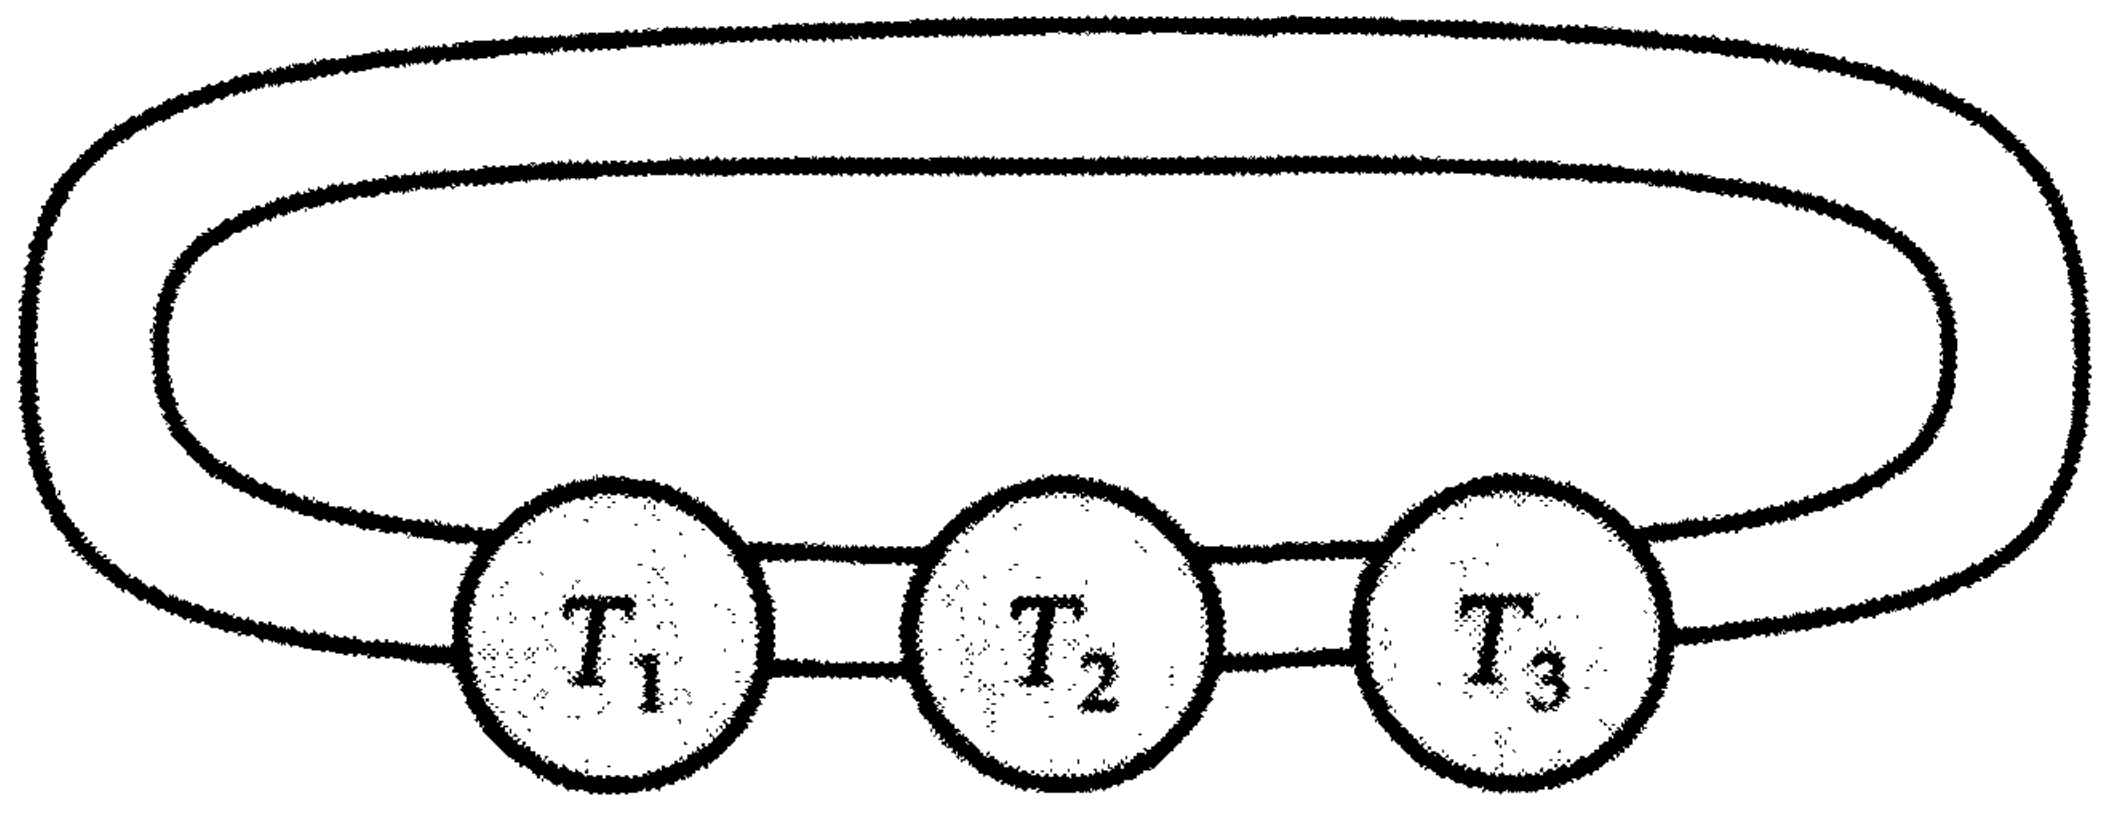
\includegraphics[width=0.8\linewidth]{Blender/ex2-25a.png}
            \caption{A knot.}
            \label{fig:ex2-25a}
        \end{subfigure}
        \begin{subfigure}[b]{0.4\linewidth}
            \centering
            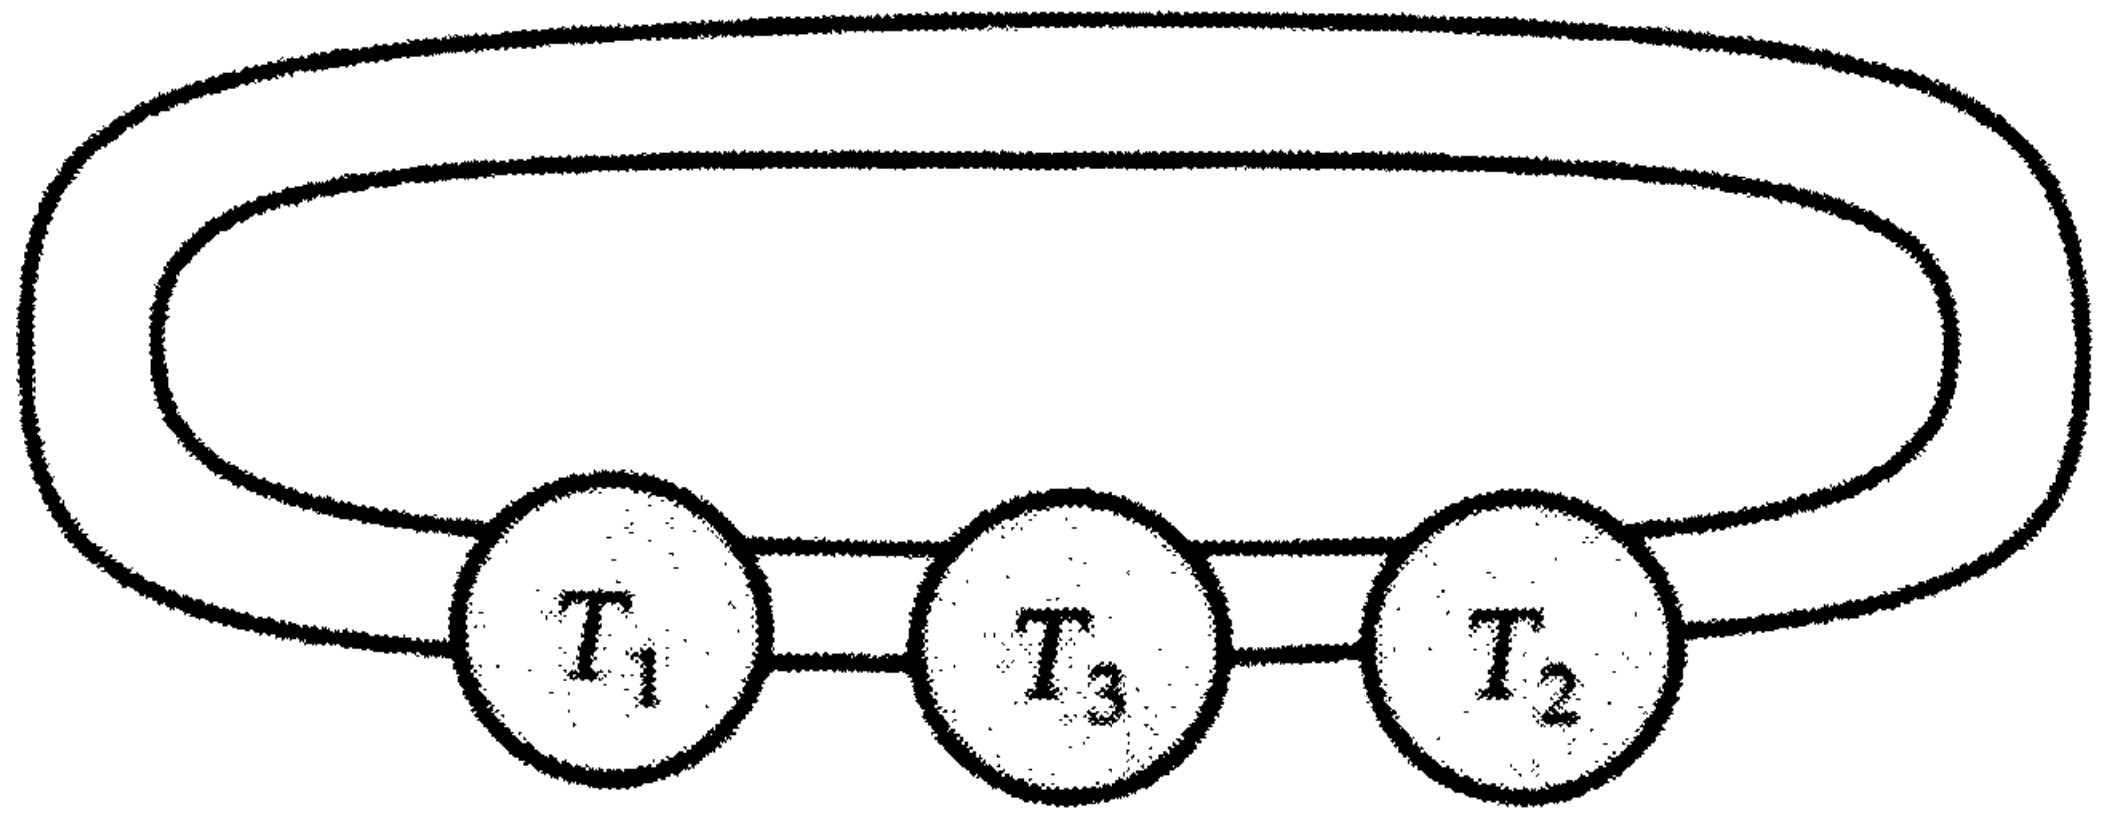
\includegraphics[width=0.8\linewidth]{Blender/ex2-25b.png}
            \caption{A mutant.}
            \label{fig:ex2-25b}
        \end{subfigure}
        \caption{Series of mutations.}
        \label{fig:ex2-9}
    \end{figure}
    \begin{itemize}
        \item Beginning in Figure \ref{fig:ex2-25a}, horizontally flip $T_2$.
        \item Horizontally flip $T_3$.
        \item Horizontally flip the unit of the flipped $T_2$ and $T_3$.
    \end{itemize}
    \item Mutation cannot turn a nontrivial knot into the trivial knot (Figure \ref{fig:circletrefoila}).
    \item More on mutant knots can be found in Sections \ref{sse:polynomials} and \ref{sse:biochemphys}.
\end{itemize}


\subsection{Knots and Planar Graphs}
\begin{itemize}
    \item This section's notation bridges knot theory and graph theory.
    \begin{itemize}
        \item It is capable of contributing to both branches of mathematics.
    \end{itemize}
    \item \textbf{Graph}: A set of points called vertices that are connected by edges.
    \item \textbf{Planar graph}: A graph that lies in a plane.
    \item Creating a planar graph from a projection of a knot or link:
    \begin{itemize}
        \item \dq{Shade every other region of the link projection so that the infinite outermost region is not shaded}{51}
        \item \dq{Put a vertex at the center of each shaded region and then connect with an edge any two vertices that are in regions that share a crossing}{52}
        \item Assign an orientation.
        \item \dq{Label each edge in the planar graph with a $+$ or a $-$, depending on whether the edge passes through a $+$ crossing or a $-$ crossing}{52} See Figure \ref{fig:crossingsign}. Recall computing link numbers in Section \ref{sss:Links} (see Figure \ref{fig:linkingnumber}, specifically).
        \item The result is a \textbf{signed planar graph}. See Figure \ref{fig:graphtrefoil} for an original example.
    \end{itemize}
    \begin{figure}[h!]
        \centering
        \begin{subfigure}[b]{0.2\linewidth}
            \centering
            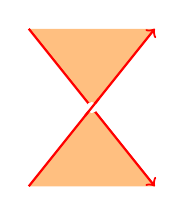
\begin{tikzpicture}
                \fill[orange!50] (-0.8,1) -- (0,0) -- (0.8,1);
                \fill[orange!50] (-0.8,-1) -- (0,0) -- (0.8,-1);
                \begin{knot}[
                    clip width=5,
                    clip radius=2pt,
                    every strand/.append style={red,thick,->}
                ]
                    \strand (-0.8,-1) to (0.8,1);
                    \strand (-0.8,1) to (0.8,-1);
                \end{knot}
            \end{tikzpicture}
            \caption{Denote $+$.}
            \label{fig:crossingsigna}
        \end{subfigure}
        \begin{subfigure}[b]{0.2\linewidth}
            \centering
            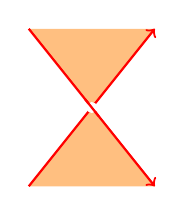
\begin{tikzpicture}
                \fill[orange!50] (-0.8,1) -- (0,0) -- (0.8,1);
                \fill[orange!50] (-0.8,-1) -- (0,0) -- (0.8,-1);
                \begin{knot}[
                    clip width=5,
                    clip radius=2pt,
                    every strand/.append style={red,thick,->},
                    flip crossing=1
                ]
                    \strand (-0.8,-1) to (0.8,1);
                    \strand (-0.8,1) to (0.8,-1);
                \end{knot}
            \end{tikzpicture}
            \caption{Denote $-$.}
            \label{fig:crossingsignb}
        \end{subfigure}
        \caption{Computing signs per crossing.}
        \label{fig:crossingsign}
    \end{figure}
    \begin{figure}[h!]
        \centering
        \begin{subfigure}[b]{0.3\linewidth}
            \centering
            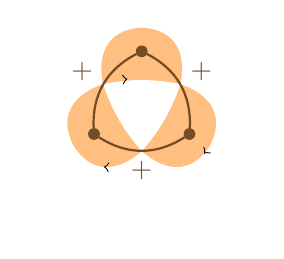
\begin{tikzpicture}
                \fill [orange!50] (90:1)
                    \foreach \x in {1,2,3} {
                        to [bend left=117,looseness=1.9] ({90+120*\x}:1)
                    }
                ;
                \fill [white] (30:0.57)
                    \foreach \x in {1,2,3} {
                        to [bend left=10] ({30-120*\x}:0.57)
                    }
                ;
    
                \begin{knot}[
                    clip width=5,
                    clip radius=2pt,
                    every strand/.append style={red,thick},
                    consider self intersections
                ]
                    \strand [
                        decoration={markings,
                        mark=at position 0.28 with {\arrow{>}},
                        mark=at position 0.48 with {\arrow{>}},
                        mark=at position 0.68 with {\arrow{>}}},
                        postaction={decorate}
                    ] (90:1)
                        \foreach \x in {1,2,3} {
                            to [bend left=117,looseness=1.9] ({90+120*\x}:1)
                        }
                    ;
                    \flipcrossings{1,3}
                \end{knot}
    
                \node (a) [circle,line width=0pt,fill=brown!60!black,inner sep=1.5pt] at (90:0.7){};
                \node (b) [circle,line width=0pt,fill=brown!60!black,inner sep=1.5pt] at (-30:0.7){}
                    edge [brown!60!black,thick,bend right=33] node[anchor=-150]{$+$} (a)
                ;
                \node (c) [circle,line width=0pt,fill=brown!60!black,inner sep=1.5pt] at (-150:0.7){}
                    edge [brown!60!black,thick,bend right=33] node[anchor=north]{$+$} (b)
                    edge [brown!60!black,thick,bend left=33]  node[anchor=-30]  {$+$} (a)
                ;
            \end{tikzpicture}
            \vspace{-0.7cm}
            \caption{Shaded trefoil projection.}
            \label{fig:graphtrefoila}
        \end{subfigure}
        \begin{subfigure}[b]{0.3\linewidth}
            \centering
            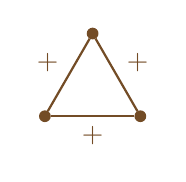
\begin{tikzpicture}
                \node (a) [circle,line width=0pt,fill=brown!60!black,inner sep=1.5pt] at (90:0.7){};
                \node (b) [circle,line width=0pt,fill=brown!60!black,inner sep=1.5pt] at (-30:0.7){}
                    edge [brown!60!black,thick] node[anchor=-150]{$+$} (a)
                ;
                \node (c) [circle,line width=0pt,fill=brown!60!black,inner sep=1.5pt] at (-150:0.7){}
                    edge [brown!60!black,thick] node[anchor=north]{$+$} (b)
                    edge [brown!60!black,thick] node[anchor=-30]  {$+$} (a)
                ;
            \end{tikzpicture}
            \vspace{-0.2cm}
            \caption{Signed planar graph.}
            \label{fig:graphtrefoilb}
        \end{subfigure}
        \caption{A signed planar graph from the standard trefoil knot projection.}
        \label{fig:graphtrefoil}
    \end{figure}
    \item It is also possible return the signed planar graph to a knot projection:
    \begin{itemize}
        \item \dq{Put an $x$ across each edge}{53}
        \item \dq{Connect the edges inside each region of the graph}{53}
        \item \dq{Shade those areas that contain a vertex}{53}
        \item \dq{At each of the $x$'s, put in a crossing corresponding to whether the edge is a $+$ edge or a $-$ edge}{53}
    \end{itemize}
    \item The significance here, as previously referenced, is that we can turn questions about knots into questions about graphs.
    \item \emph{Exercise 2.31}: What do the Reidemeister moves become when translated into operations on signed planar graphs? (Make sure you consider what happens when different regions are shaded.)
    \begin{itemize}
        \item Type I Reidemeister move: Extend an edge from one vertex to a newly created one. Either sign is acceptable (the sign option is analogous to the over-under crossing option).
        \item Type II Reidemeister move: Add two edges connecting two, specific vertices and intersecting no other edges. The signs on the new edges must be opposite, but it either can be positive (or negative; this option is analogous to the over-under crossing option).
        \item Type III Reidemeister move: I do not know$^[$\footnote{Return to this later.}$^]$.
    \end{itemize}
    \item See Section \ref{sss:StatisticalMechanics} for more on signed planar graphs.
\end{itemize}
\newpage



\section{Invariants of Knots}
\subsection{Unknotting Number}\label{sss:UnknottingNumber}
\begin{itemize}
    \item \textbf{Unknotting number}: A value $n\in\mathbb{N}$ specific to a knot $K$ that gives the fewest number of crossing changes needed in any projection to turn it into the unknot. \emph{Also known as} $\mathbf{u(K)}$.
    \begin{itemize}
        \item It may, however, be a nasty projection of the unknot (see Figure \ref{fig:ex1-11-2} and the related Exercise).
    \end{itemize}
    \item \emph{Exercise 3.1}: Find the unknotting number of the figure-eight knot (Figure \ref{fig:figure8knot}).
    \begin{itemize}
        \item $u(K)=1$, where $K$ is the figure-eight knot.
        \item $K$ is distinct from the unknot, so $u(K)\neq 0$. The next possibility ($u(K)=1$) succeeds with the projection in Figure \ref{fig:figure8knot} (in fact, flipping \emph{any} crossing in the referenced projection trivializes $K$).
    \end{itemize}
    \item Note that performing all of the crossing changes on one projection is equivalent to performing one such change, then an ambient isotropy, then another\dots
    \begin{itemize}
        \item A proof of this is listed on page 58.
    \end{itemize}
    \item \dq{The fact that every knot has a finite unknotting number follows from the fact that every projection of a knot can be changed into a projection of the unknot by changing some subset of the crossings in the projection}{58}
    \begin{itemize}
        \item See \emph{Exercise 1.7}.
    \end{itemize}
    \item A proof of the above:
    \begin{itemize}
        \item Pick a starting point (not a crossing) on an arbitrary knot and an orientation in whose direction to traverse the knot.
        \item When you arrive at the first crossing, change it so that the strand that you are on is the over strand, if necessary.
        \item Continue changing every new crossing to which you come to make the current strand into the overstrand.
        \begin{itemize}
            \item Do not change crossings that you have already passed through once.
        \end{itemize}
        \item At this point, you now have a projection of a knot that was obtained from the original knot by changing crossings and that is the trivial knot. A proof of this triviality follows.
        \medskip
        \item Consider the knot in three-space, with the $z$-axis coming out of the page. Assign to the starting point the $z$-coordinate, $z=1$.
        \item Decrease the $z$-coordinate of each consecutive point as you traverse the knot, culminating in the original point being labeled, $z=0$.
        \begin{itemize}
            \item Connect the starting and ending points with a vertical bar to preserve the knot as a knot.
        \end{itemize}
        \item What you have now obtained is a knot in three-space that, when projected from the top is the knot that we constructed before the line break, but has no crossings when projected from the side (and is therefore the trivial knot).
        \item Q.E.D.
    \end{itemize}
    \item It is very hard, in general, to find the unknotting number of a knot. How do you know that there isn't a better projection?
    \item \dq{A knot with unknotting number 1 is prime}{61}
    \item Therefore, a composite knot cannot be unknotted with a one crossing change.
    \begin{itemize}
        \item Another way to think about this idea is that changing a crossing to unknot one factor knot would yield the composition of the other factor knot with the unknot, which, according to Section \ref{sss:Composition}, is simply the other factor knot (obviously still fully knotted).
    \end{itemize}
    \begin{equation}
        u(K_1\#K_2)\leq u(K_1)+u(K_2)
    \end{equation}
    \item The unknotting number can be realized by a projection that is not \textbf{minimal}.
    \item \textbf{Minimal projection}: The projection of a knot with the lowest possible number of crossings.
    \item \textbf{\emph{k}-move}: A local change in the projection that replaces two untwisted strings with two strings that twist around each other with $k$ crossings in a right-handed manner. See Figure \ref{fig:k-moves}.
    \begin{itemize}
        \item If $k$ is positive, then the overstrand has a positive slope.
    \end{itemize}
    \begin{figure}[h!]
        \centering
        \begin{subfigure}[b]{0.2\linewidth}
            \centering
            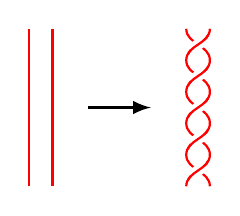
\begin{tikzpicture}[
                every to/.style={out=90,in=-90}
            ]
                \def\val{0.15}
                \begin{scope}[red, thick, xshift=-1cm]
                    \draw (-\val,-1) -- (-\val,1);
                    \draw (\val,-1) -- (\val,1);
                \end{scope}
                \draw[very thick,-latex] (-0.4,0) -- (0.4,0);
                \begin{knot}[
                    clip width=5,
                    clip radius=3pt,
                    every strand/.append style={red,thick},
                    xshift=1cm,
                    ignore endpoint intersections=false
                ]
                    \strand (-\val,-1) to (\val,-0.6) to (-\val,-0.2) to (\val,0.2) to (-\val,0.6) to (\val,1);
                    \strand (\val,-1) to (-\val,-0.6) to (\val,-0.2) to (-\val,0.2) to (\val,0.6) to (-\val,1);
                    \flipcrossings{2,4}
                \end{knot}
            \end{tikzpicture}
            \caption{A 5-move.}
            \label{fig:k-movesa}
        \end{subfigure}
        \begin{subfigure}[b]{0.2\linewidth}
            \centering
            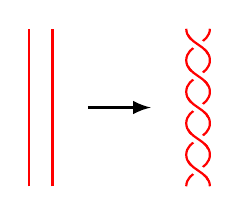
\begin{tikzpicture}[
                every to/.style={out=90,in=-90}
            ]
                \def\val{0.15}
                \begin{scope}[red, thick, xshift=-1cm]
                    \draw (-\val,-1) -- (-\val,1);
                    \draw (\val,-1) -- (\val,1);
                \end{scope}
                \draw[very thick,-latex] (-0.4,0) -- (0.4,0);
                \begin{knot}[
                    clip width=5,
                    clip radius=3pt,
                    every strand/.append style={red,thick},
                    xshift=1cm,
                    ignore endpoint intersections=false
                ]
                    \strand (\val,-1) to (-\val,-0.6) to (\val,-0.2) to (-\val,0.2) to (\val,0.6) to (-\val,1);
                    \strand (-\val,-1) to (\val,-0.6) to (-\val,-0.2) to (\val,0.2) to (-\val,0.6) to (\val,1);
                    \flipcrossings{2,4}
                \end{knot}
            \end{tikzpicture}
            \caption{A $-5$-move.}
            \label{fig:k-movesb}
        \end{subfigure}
        \caption{Examples of $k$-moves.}
        \label{fig:k-moves}
    \end{figure}
    \item \textbf{\emph{k}-equivalent}: Two knot or link projections that can be transformed into each other through a series of $k$-moves and $-k$-moves.
    \begin{itemize}
        \item Ambient isotropies are allowed between $k$-moves.
    \end{itemize}
    \item \emph{Exercise 3.8}: Show that the knots in Figure \ref{fig:ex3-8} are each three-equivalent to a trivial link.
    \begin{figure}[h!]
        \centering
        \begin{subfigure}[b]{0.3\linewidth}
            \centering
            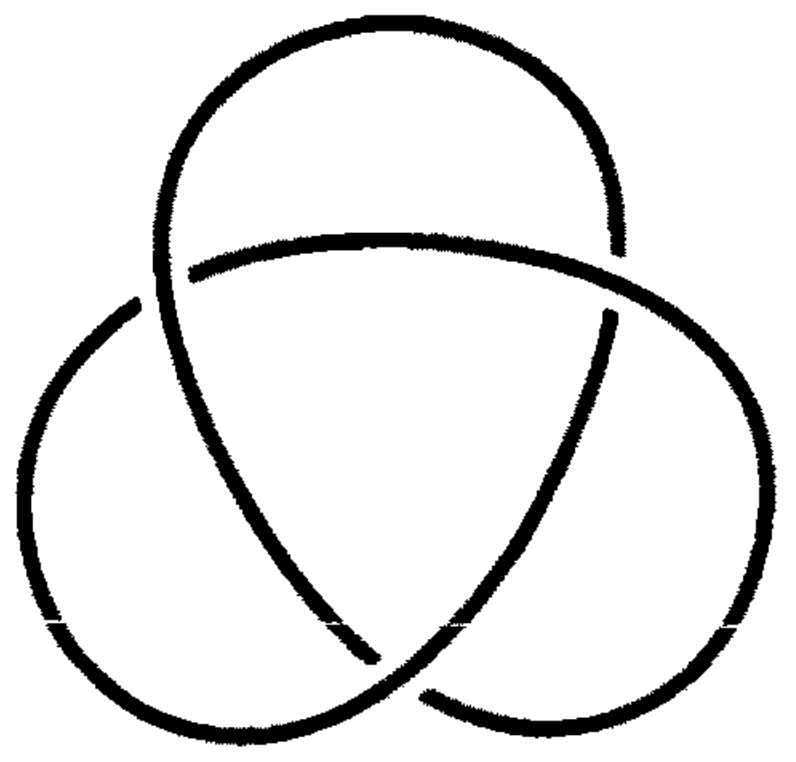
\includegraphics[width=0.5\linewidth]{Blender/ex3-8a.png}
            \caption{The knot $3_1$.}
            \label{fig:ex3-8a}
        \end{subfigure}
        \begin{subfigure}[b]{0.3\linewidth}
            \centering
            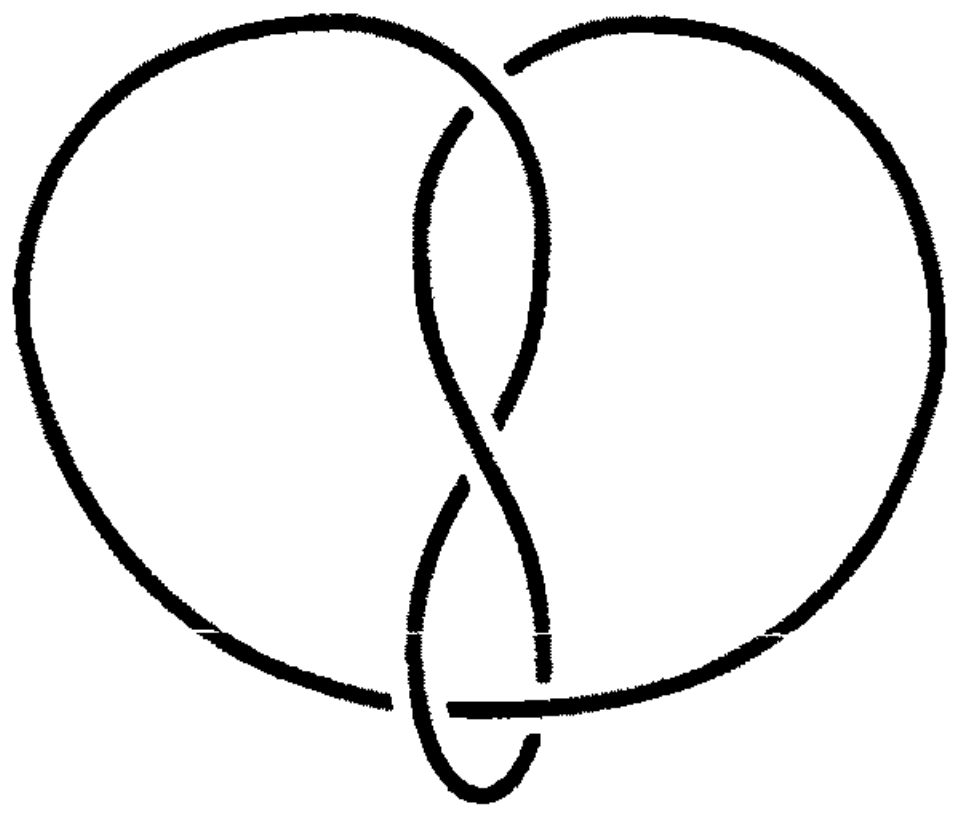
\includegraphics[width=0.55\linewidth]{Blender/ex3-8b.png}
            \caption{The knot $4_1$.}
            \label{fig:ex3-8b}
        \end{subfigure}
        \caption{Knots that are 3-equivalent to trivial links.}
        \label{fig:ex3-8}
    \end{figure}
    \begin{figure}[h!]
        \centering
        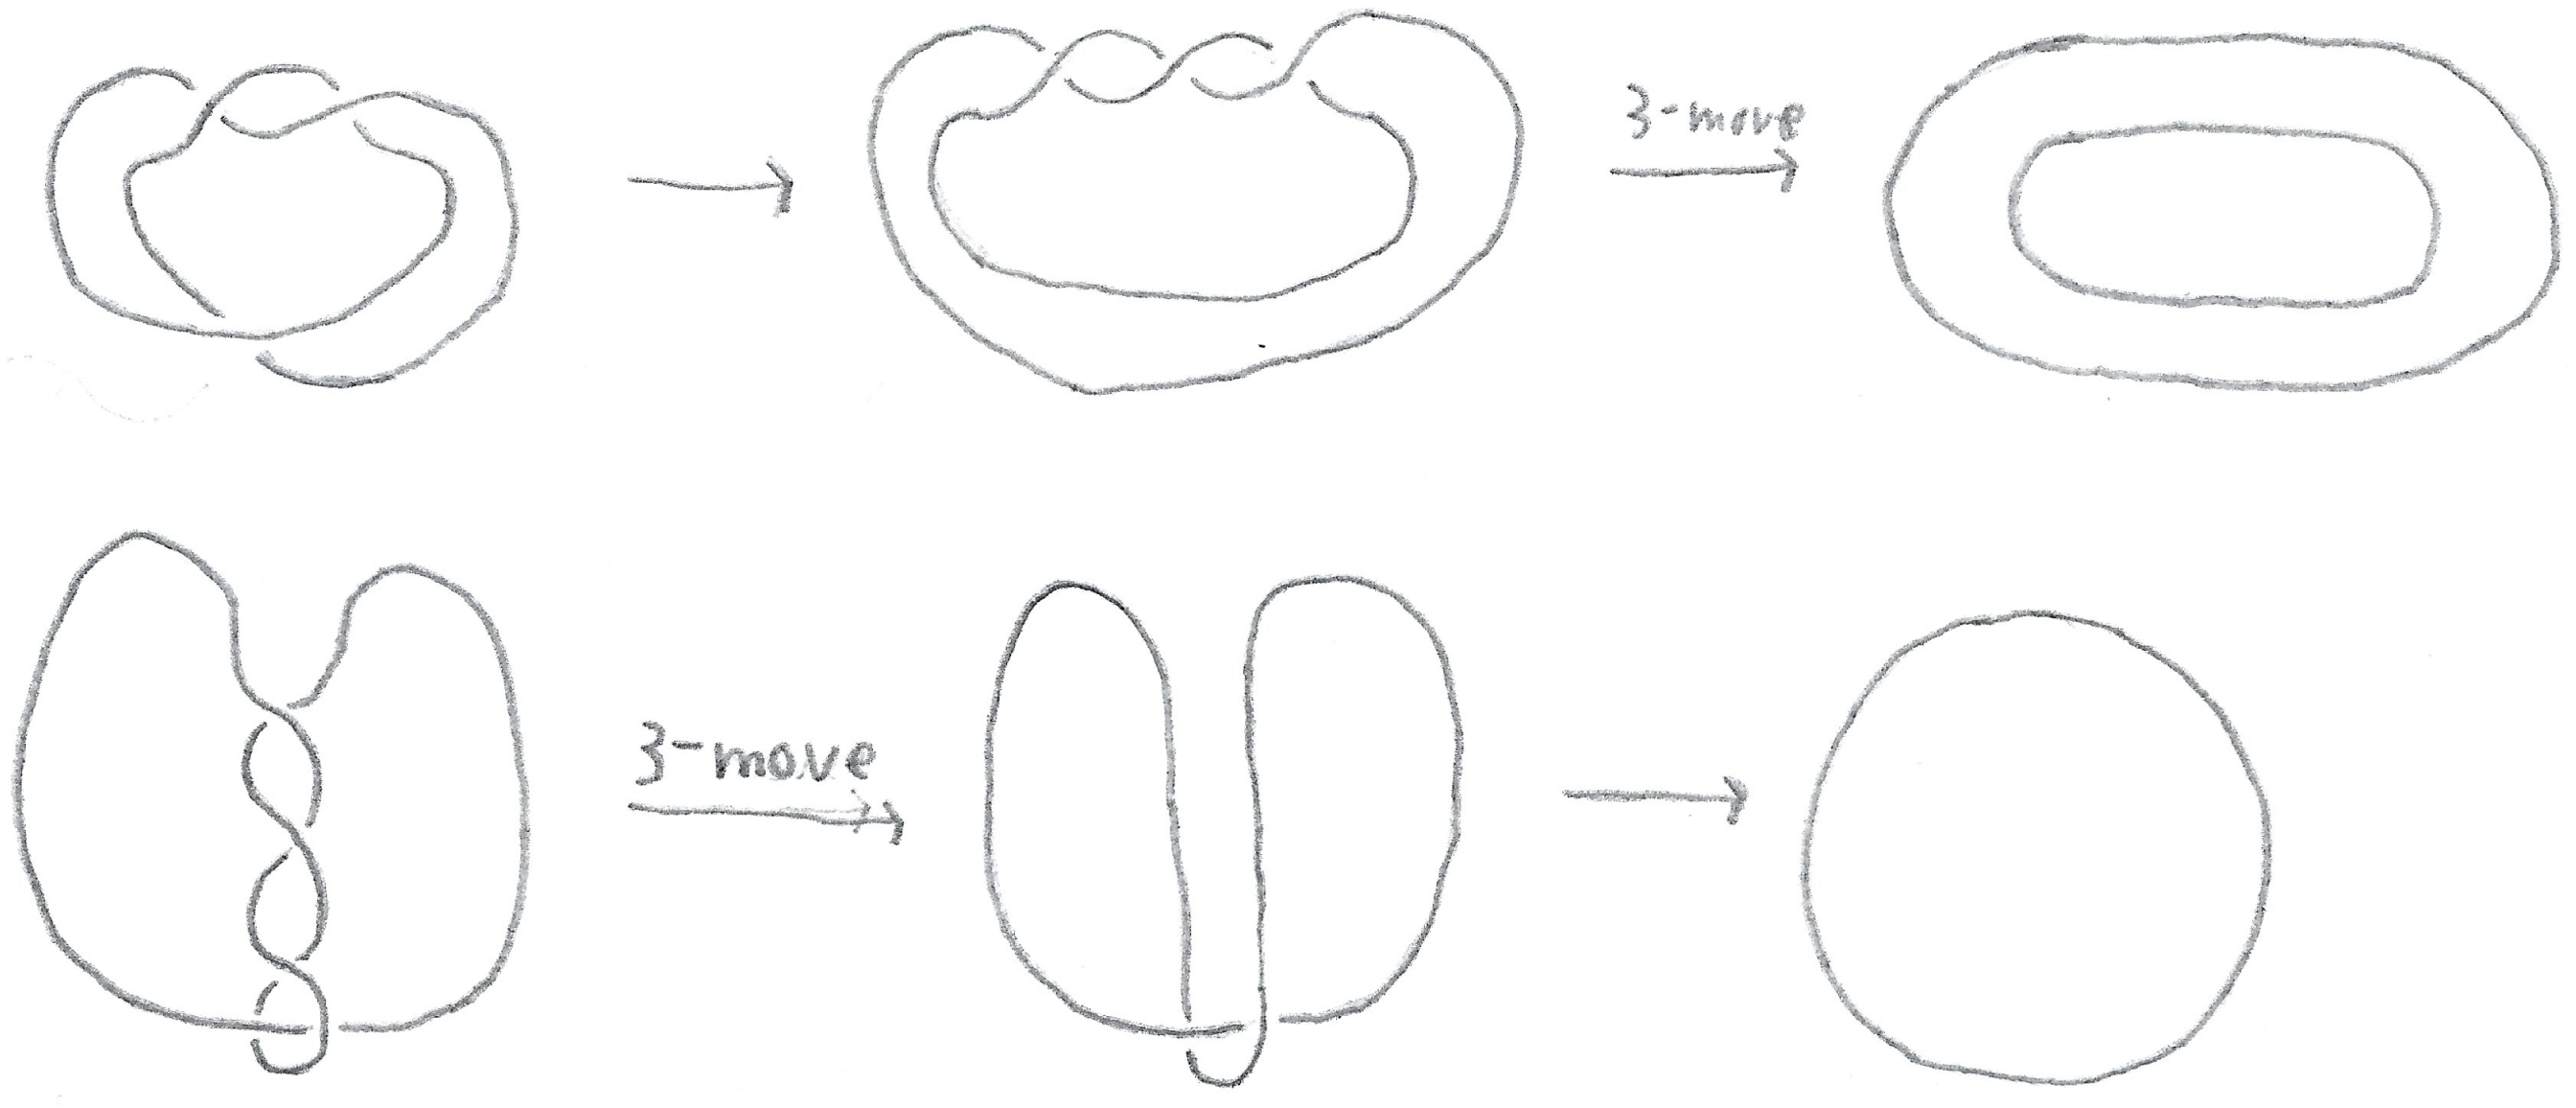
\includegraphics[width=0.7\linewidth]{Blender/ex3-8-2.png}
        \caption{Solution to \emph{Exercise 3.8}.}
        \label{fig:ex3-8-2}
    \end{figure}
\end{itemize}


\subsection{Bridge Number}\label{sss:Bridge}
\begin{itemize}
    \item Think of knots as \dq{cutting through the projection plane, rather than lying in it}{64}
    \begin{itemize}
        \item Every overstrand is entirely above and every understrand is entirely beneath. The points where the strand shifts from over to under are known as \textbf{vertices}.
    \end{itemize}
    \item \textbf{Bridge number}: The least number of unknotted arcs lying above the plane in any projection of the knot. \emph{Also known as} $\mathbf{b(K)}$
    \begin{itemize}
        \item The number of maximal overpasses in in the projection.
    \end{itemize}
    \item \textbf{Overpass}: \dq{A subarc of the knot that goes over at least one crossing but never goes under a crossing}{64}
    \item \textbf{Maximal overpass}: \dq{An overpass that could not be made any longer}{65}
    \begin{figure}[h!]
        \centering
        \begin{subfigure}[b]{0.4\linewidth}
            \centering
            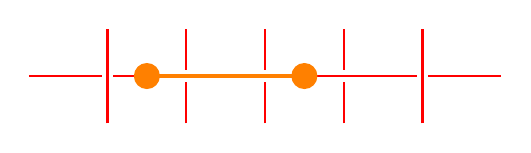
\begin{tikzpicture}[dot/.style={circle,fill=orange,outer sep=-1pt}]
                \def\val{0.6}
                \begin{knot}[
                    clip width=5,
                    every strand/.append style={red,thick}
                ]
                    \strand (0,0) to (6,0);
                    \strand (1,-\val) to (1,\val);
                    \strand (2,-\val) to (2,\val);
                    \strand (3,-\val) to (3,\val);
                    \strand (4,-\val) to (4,\val);
                    \strand (5,-\val) to (5,\val);
                    \flipcrossings{1,5}
                \end{knot}
                \node [dot] (a) at (1.5,0) {};
                \node [dot] (b) at (3.5,0) {}
                    edge [ultra thick,orange] (a)
                ;
            \end{tikzpicture}
            \caption{An overpass.}
            \label{fig:overpassa}
        \end{subfigure}
        \begin{subfigure}[b]{0.4\linewidth}
            \centering
            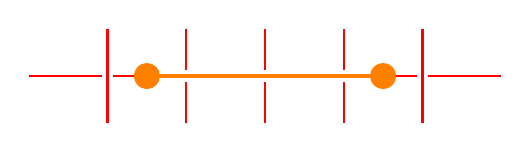
\begin{tikzpicture}[dot/.style={circle,fill=orange,outer sep=-1pt}]
                \def\val{0.6}
                \begin{knot}[
                    clip width=5,
                    every strand/.append style={red,thick}
                ]
                    \strand (0,0) to (6,0);
                    \strand (1,-\val) to (1,\val);
                    \strand (2,-\val) to (2,\val);
                    \strand (3,-\val) to (3,\val);
                    \strand (4,-\val) to (4,\val);
                    \strand (5,-\val) to (5,\val);
                    \flipcrossings{1,5}
                \end{knot}
                \node [dot] (a) at (1.5,0) {};
                \node [dot] (b) at (4.5,0) {}
                    edge [ultra thick,orange] (a)
                ;
            \end{tikzpicture}
            \caption{A maximal overpass.}
            \label{fig:overpassb}
        \end{subfigure}
        \caption{Overpasses.}
        \label{fig:overpass}
    \end{figure}
    \item \emph{Exercise 3.10}: Show that if a knot has bridge number 1, it must be the unknot.
    \begin{itemize}
        \item If a knot has bridge number 1, $\exists$ a projection of the knot such that there is only one arc above the projection plane and 1 arc below the projection plane.
        \item This projection, viewed from above, will look like any isotropy of the knot. However, viewed from the side, there will be 0 crossings --- therefore, it is the unknot.
    \end{itemize}
    \item \emph{Exercise 3.11}: Show that the knot $5_2$ has bridge number 2$^[$\footnote{Idea for a paper: On reducing bridge number. Discuss manipulating a projection to its Dowker reconstruction to create the "killzone" and then using "bridging moves" to make the projection nonalternating. 2 types so far: I $\rightarrow$ III, and 2xII $\rightarrow$ III (in both cases it is the Type III move which climactically changes $b(K)$. It can be necessary to increase $b(K)$ before decreasing it.)}$^]$.
    \begin{itemize}
        \item Since $5_2$ is distinct from the unknot, $b(K)\neq 1$.
        \item Therefore, the next possibility to check is 2. If $\exists$ a projection of $5_2$ with bridge number 2, $b(K)=2$.
        \begin{figure}[h!]
            \centering
            \begin{subfigure}[b]{0.2\linewidth}
                \centering
                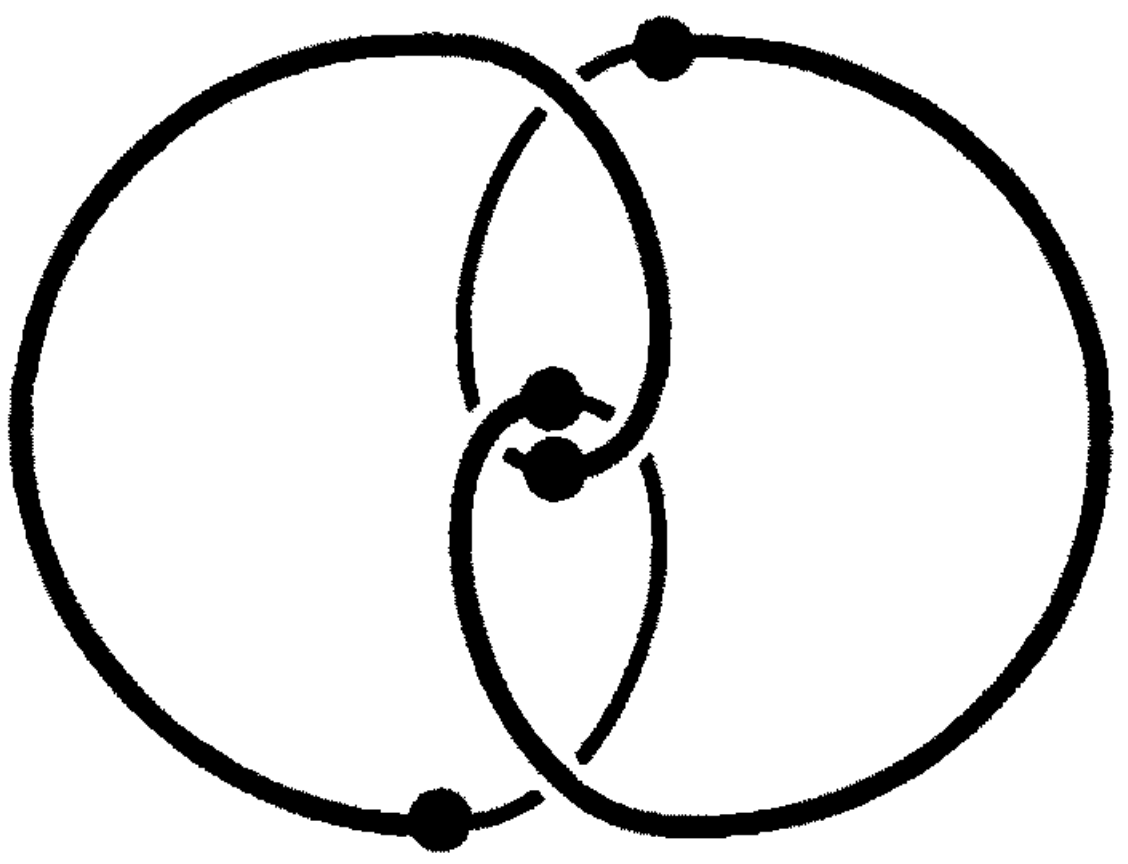
\includegraphics[width=0.8\linewidth]{Blender/ex3-11a.png}
                \caption{$3_1$ with $b(K)=2$.}
                \label{fig:ex3-11a}
            \end{subfigure}
            \begin{subfigure}[b]{0.2\linewidth}
                \centering
                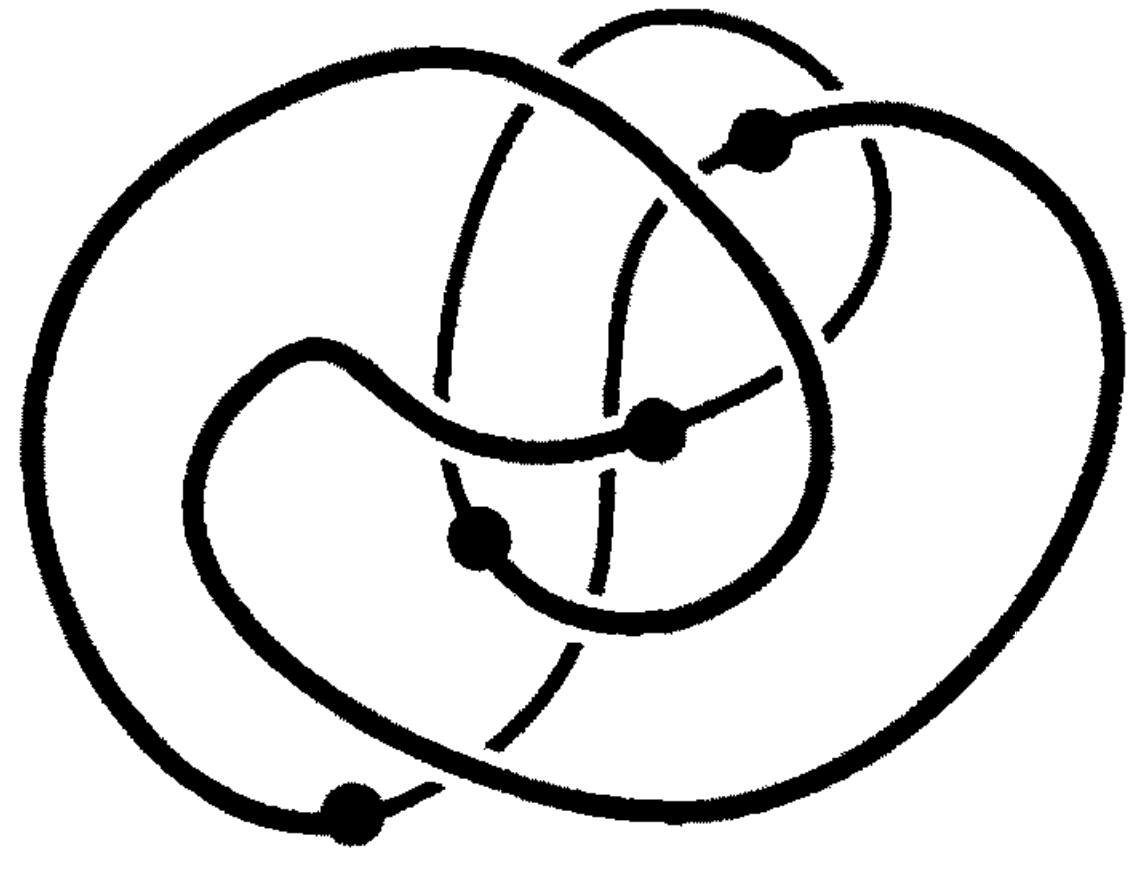
\includegraphics[width=0.8\linewidth]{Blender/ex3-11b.png}
                \caption{$4_1$ with $b(K)=2$.}
                \label{fig:ex3-11b}
            \end{subfigure}
            \caption{Reducing bridge number between projections.}
            \label{fig:ex3-11}
        \end{figure}
        \item Before tackling this problem, though, let's look at some simpler examples.
        \begin{itemize}
            \item From these, we notice that there are "bridging moves" (distinct combinations of the Reidemeister moves) that can shift the bridge number by $\pm 1$.
            \item Furthermore, long overstrands call to mind a Dowker reconstruction (Figure \ref{fig:reconstruction}).
        \end{itemize}
        \item Find the Dowker notation of $5_2$.
        \begin{itemize}
            \item The Dowker notation of the projection listed in the appendix is 6 10 8 2 4.
        \end{itemize}
        \begin{figure}[h!]
            \centering
            \begin{subfigure}[b]{0.3\linewidth}
                \centering
                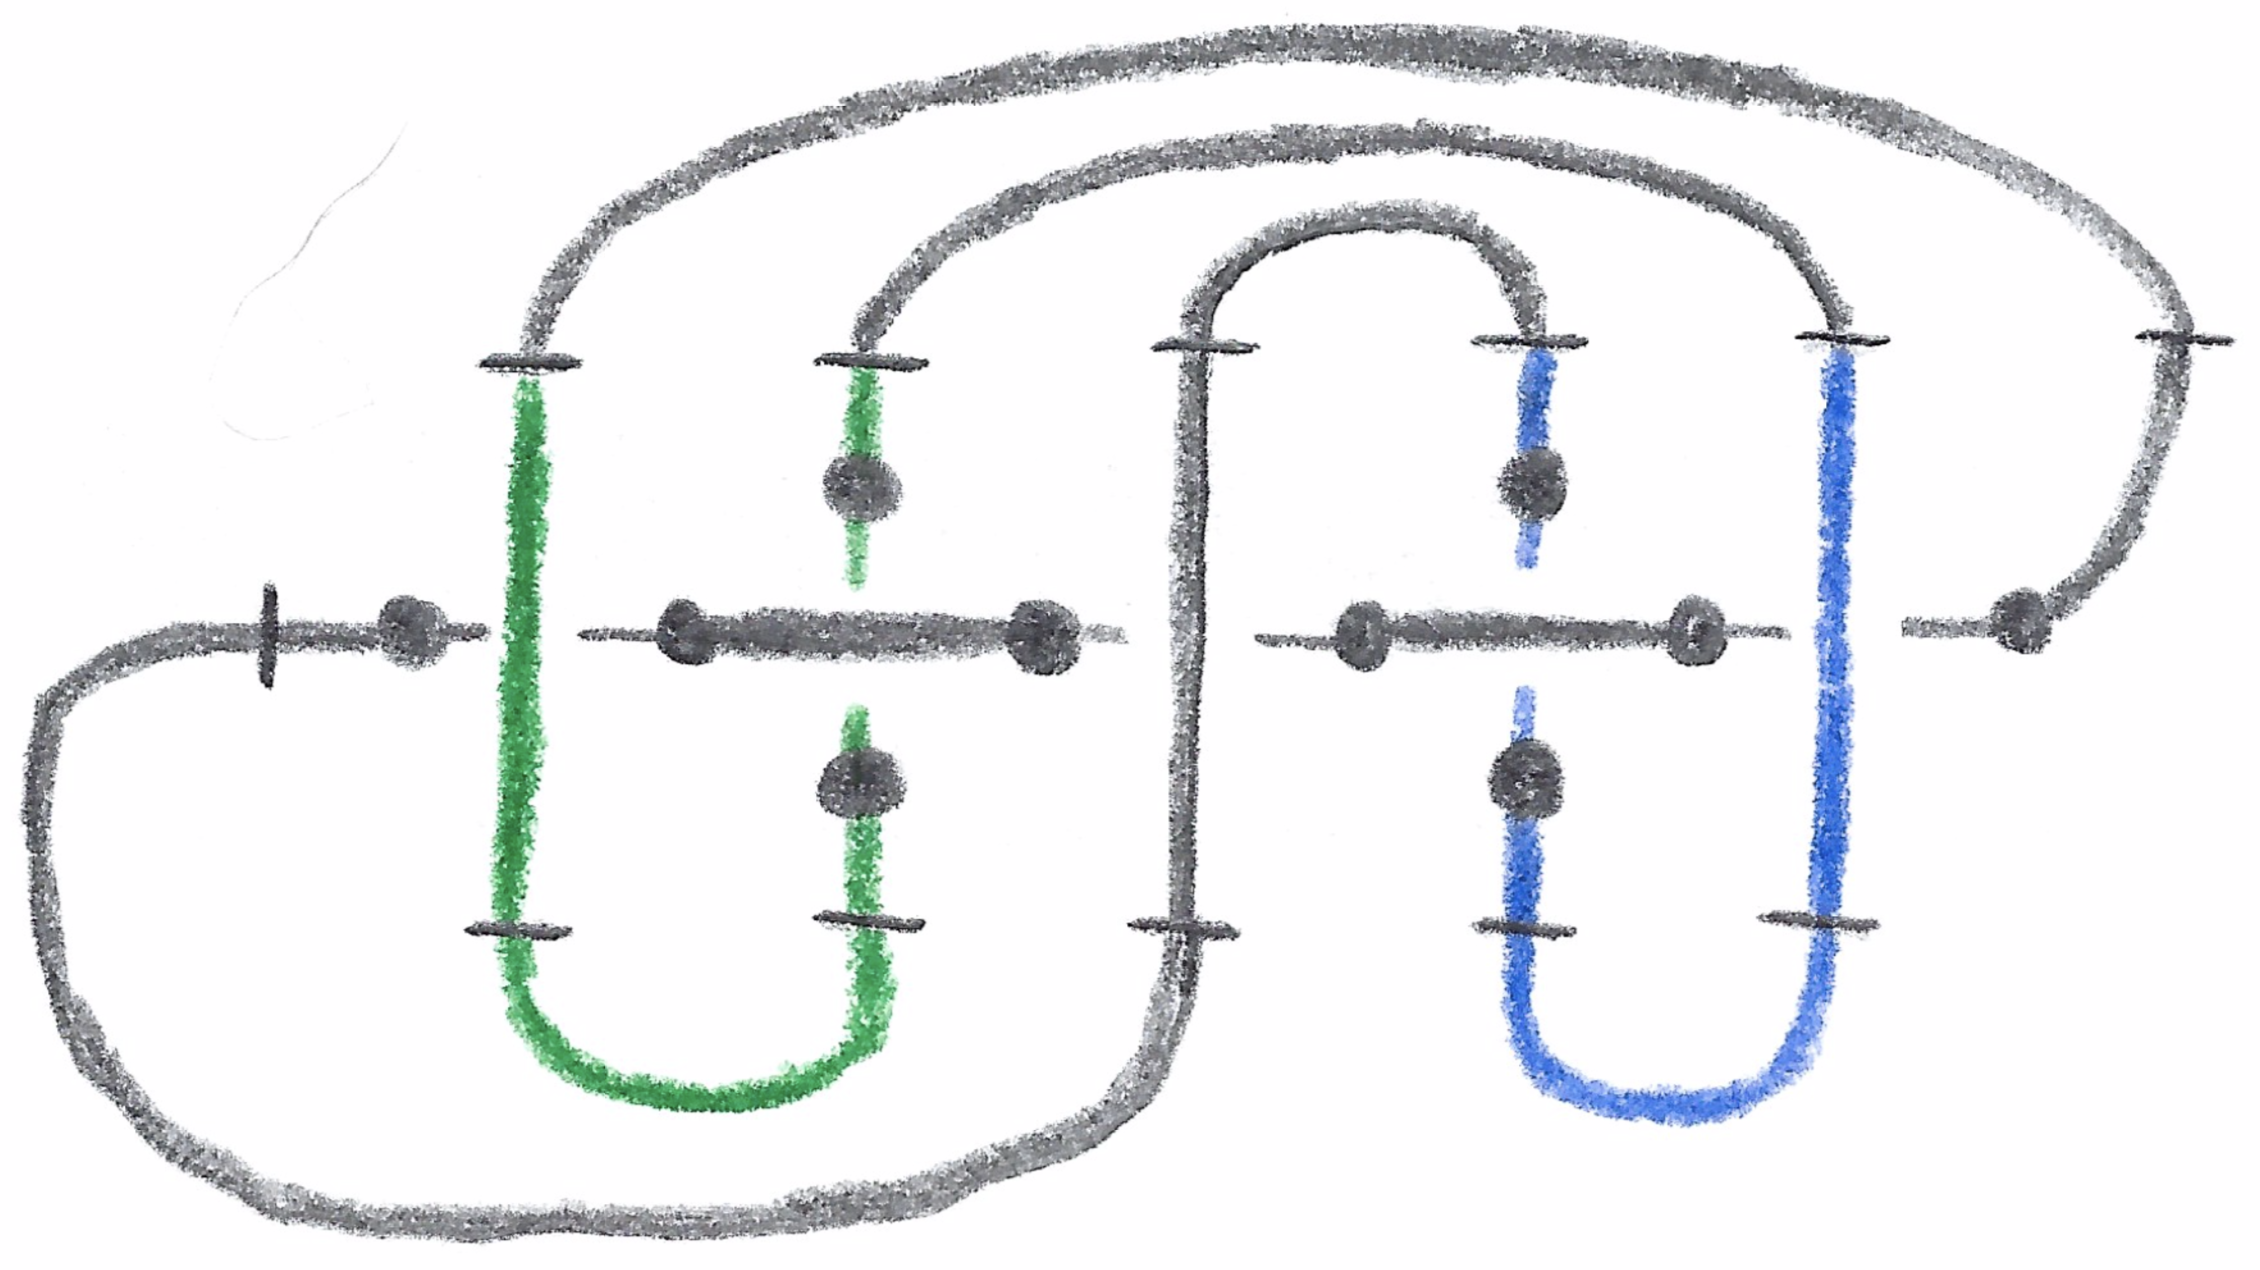
\includegraphics[width=0.8\linewidth]{Blender/ex3-11-2a.png}
                \caption{Bridge number: 5.}
                \label{fig:ex3-11-2a}
            \end{subfigure}
            \begin{subfigure}[b]{0.3\linewidth}
                \centering
                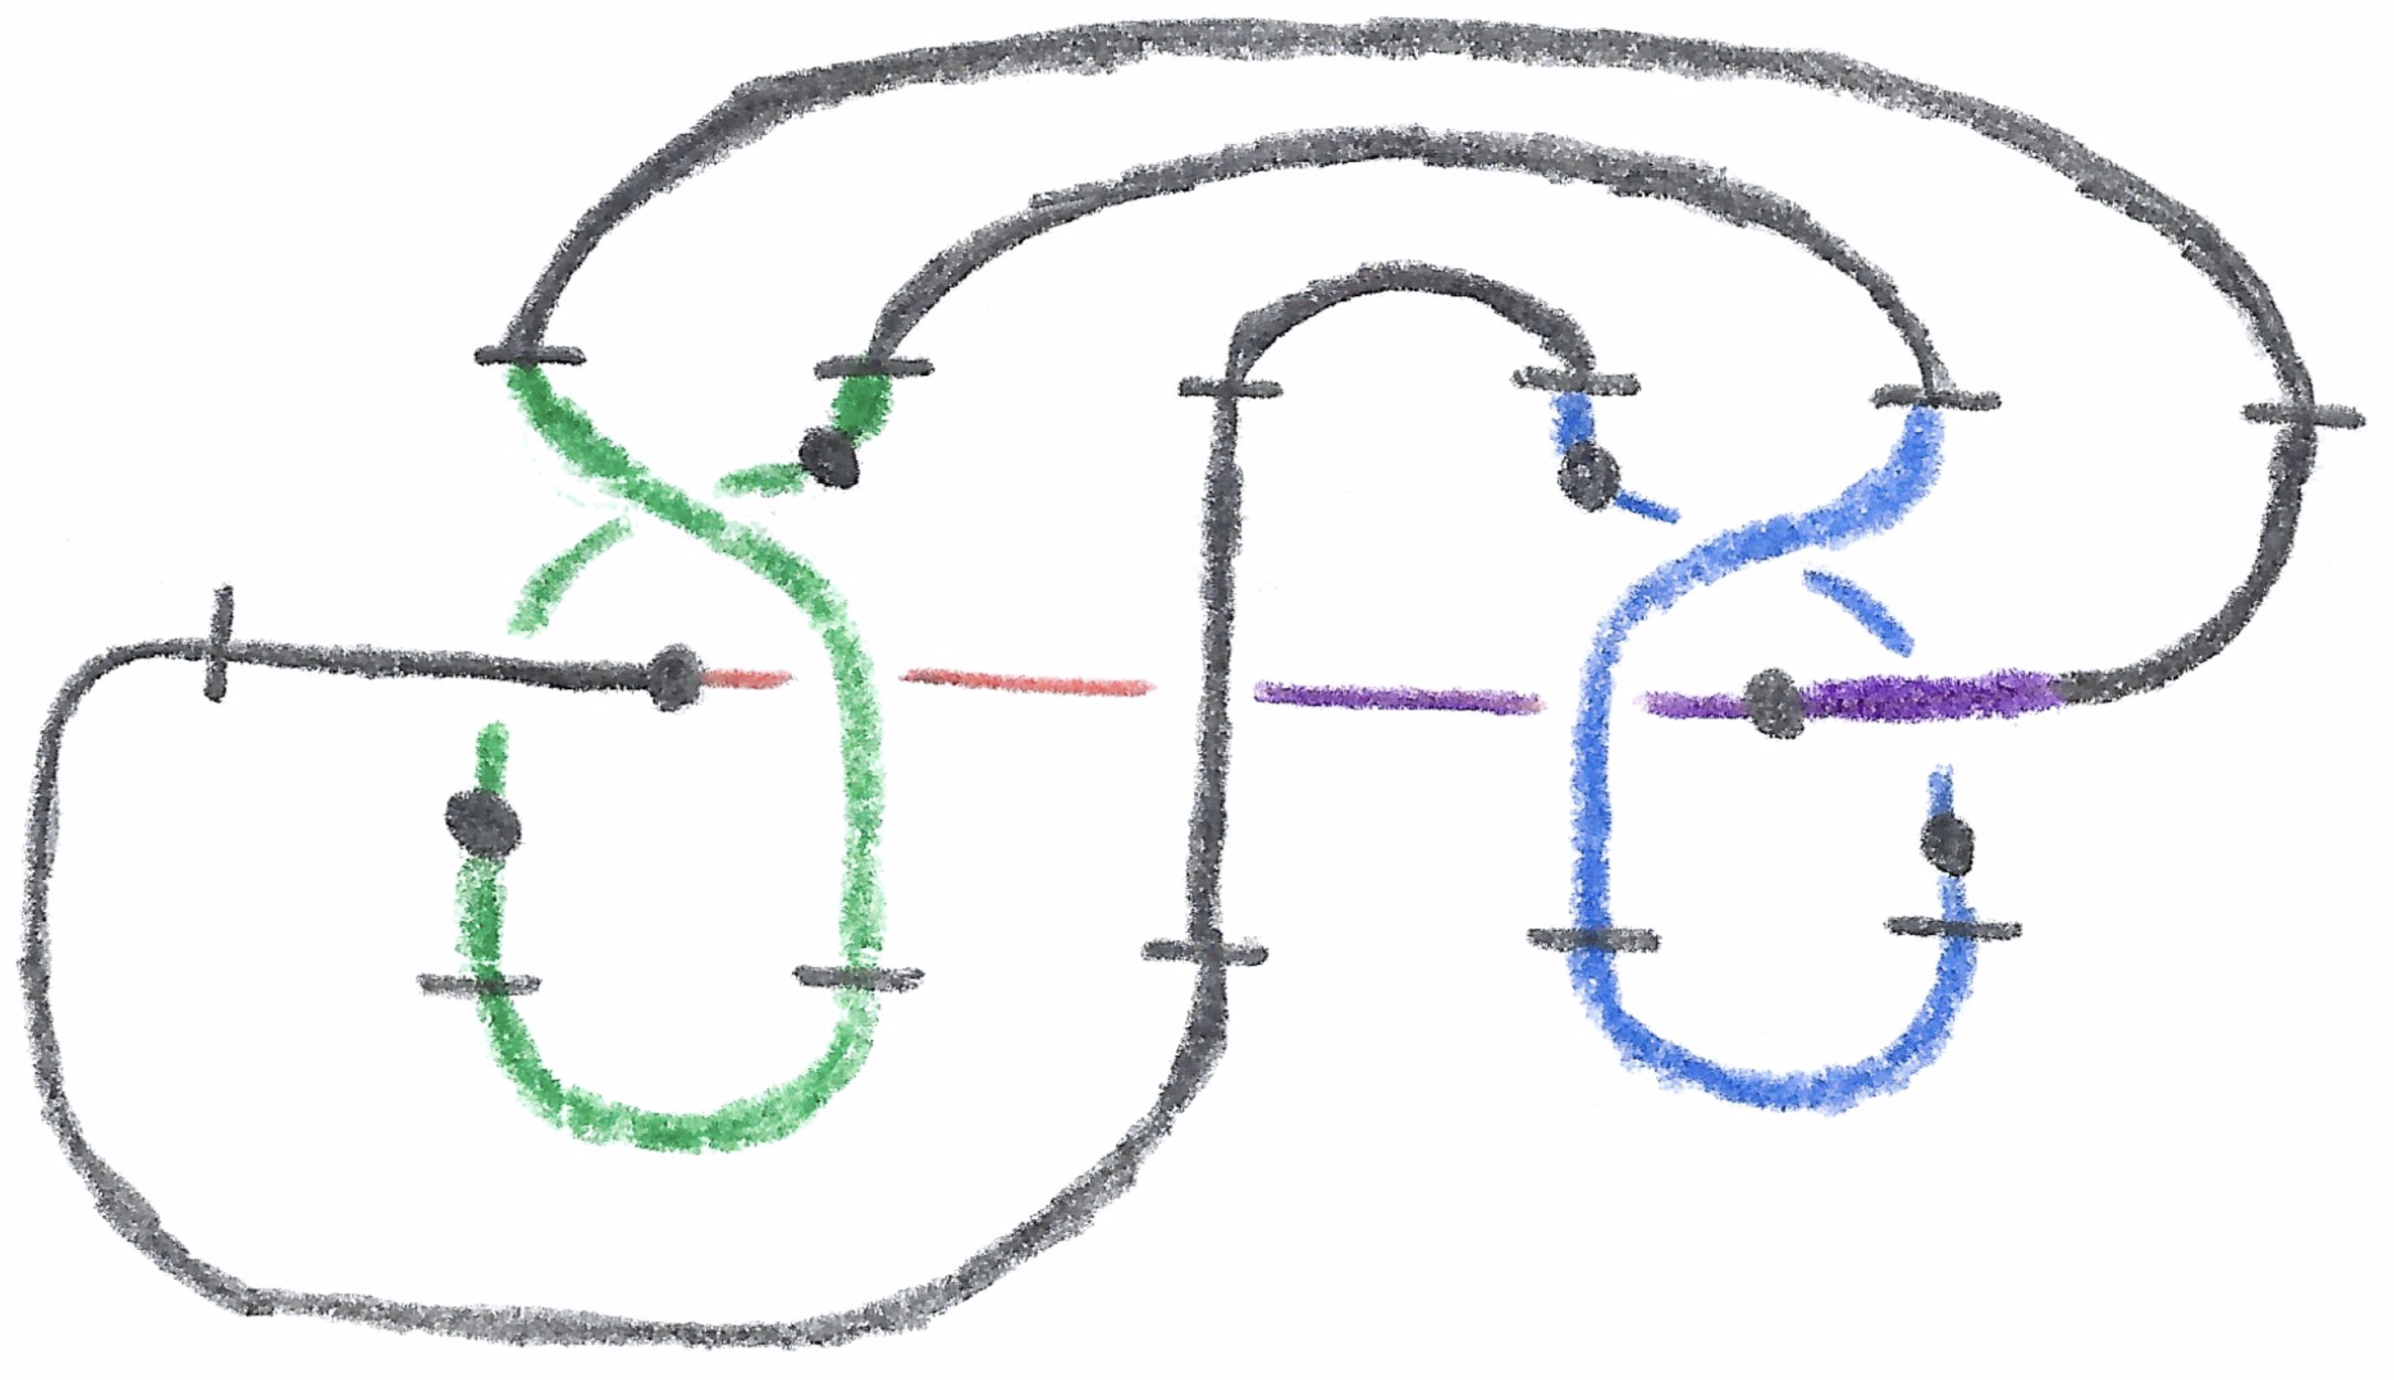
\includegraphics[width=0.8\linewidth]{Blender/ex3-11-2b.png}
                \caption{Bridge number: 3.}
                \label{fig:ex3-11-2b}
            \end{subfigure}
            \begin{subfigure}[b]{0.3\linewidth}
                \centering
                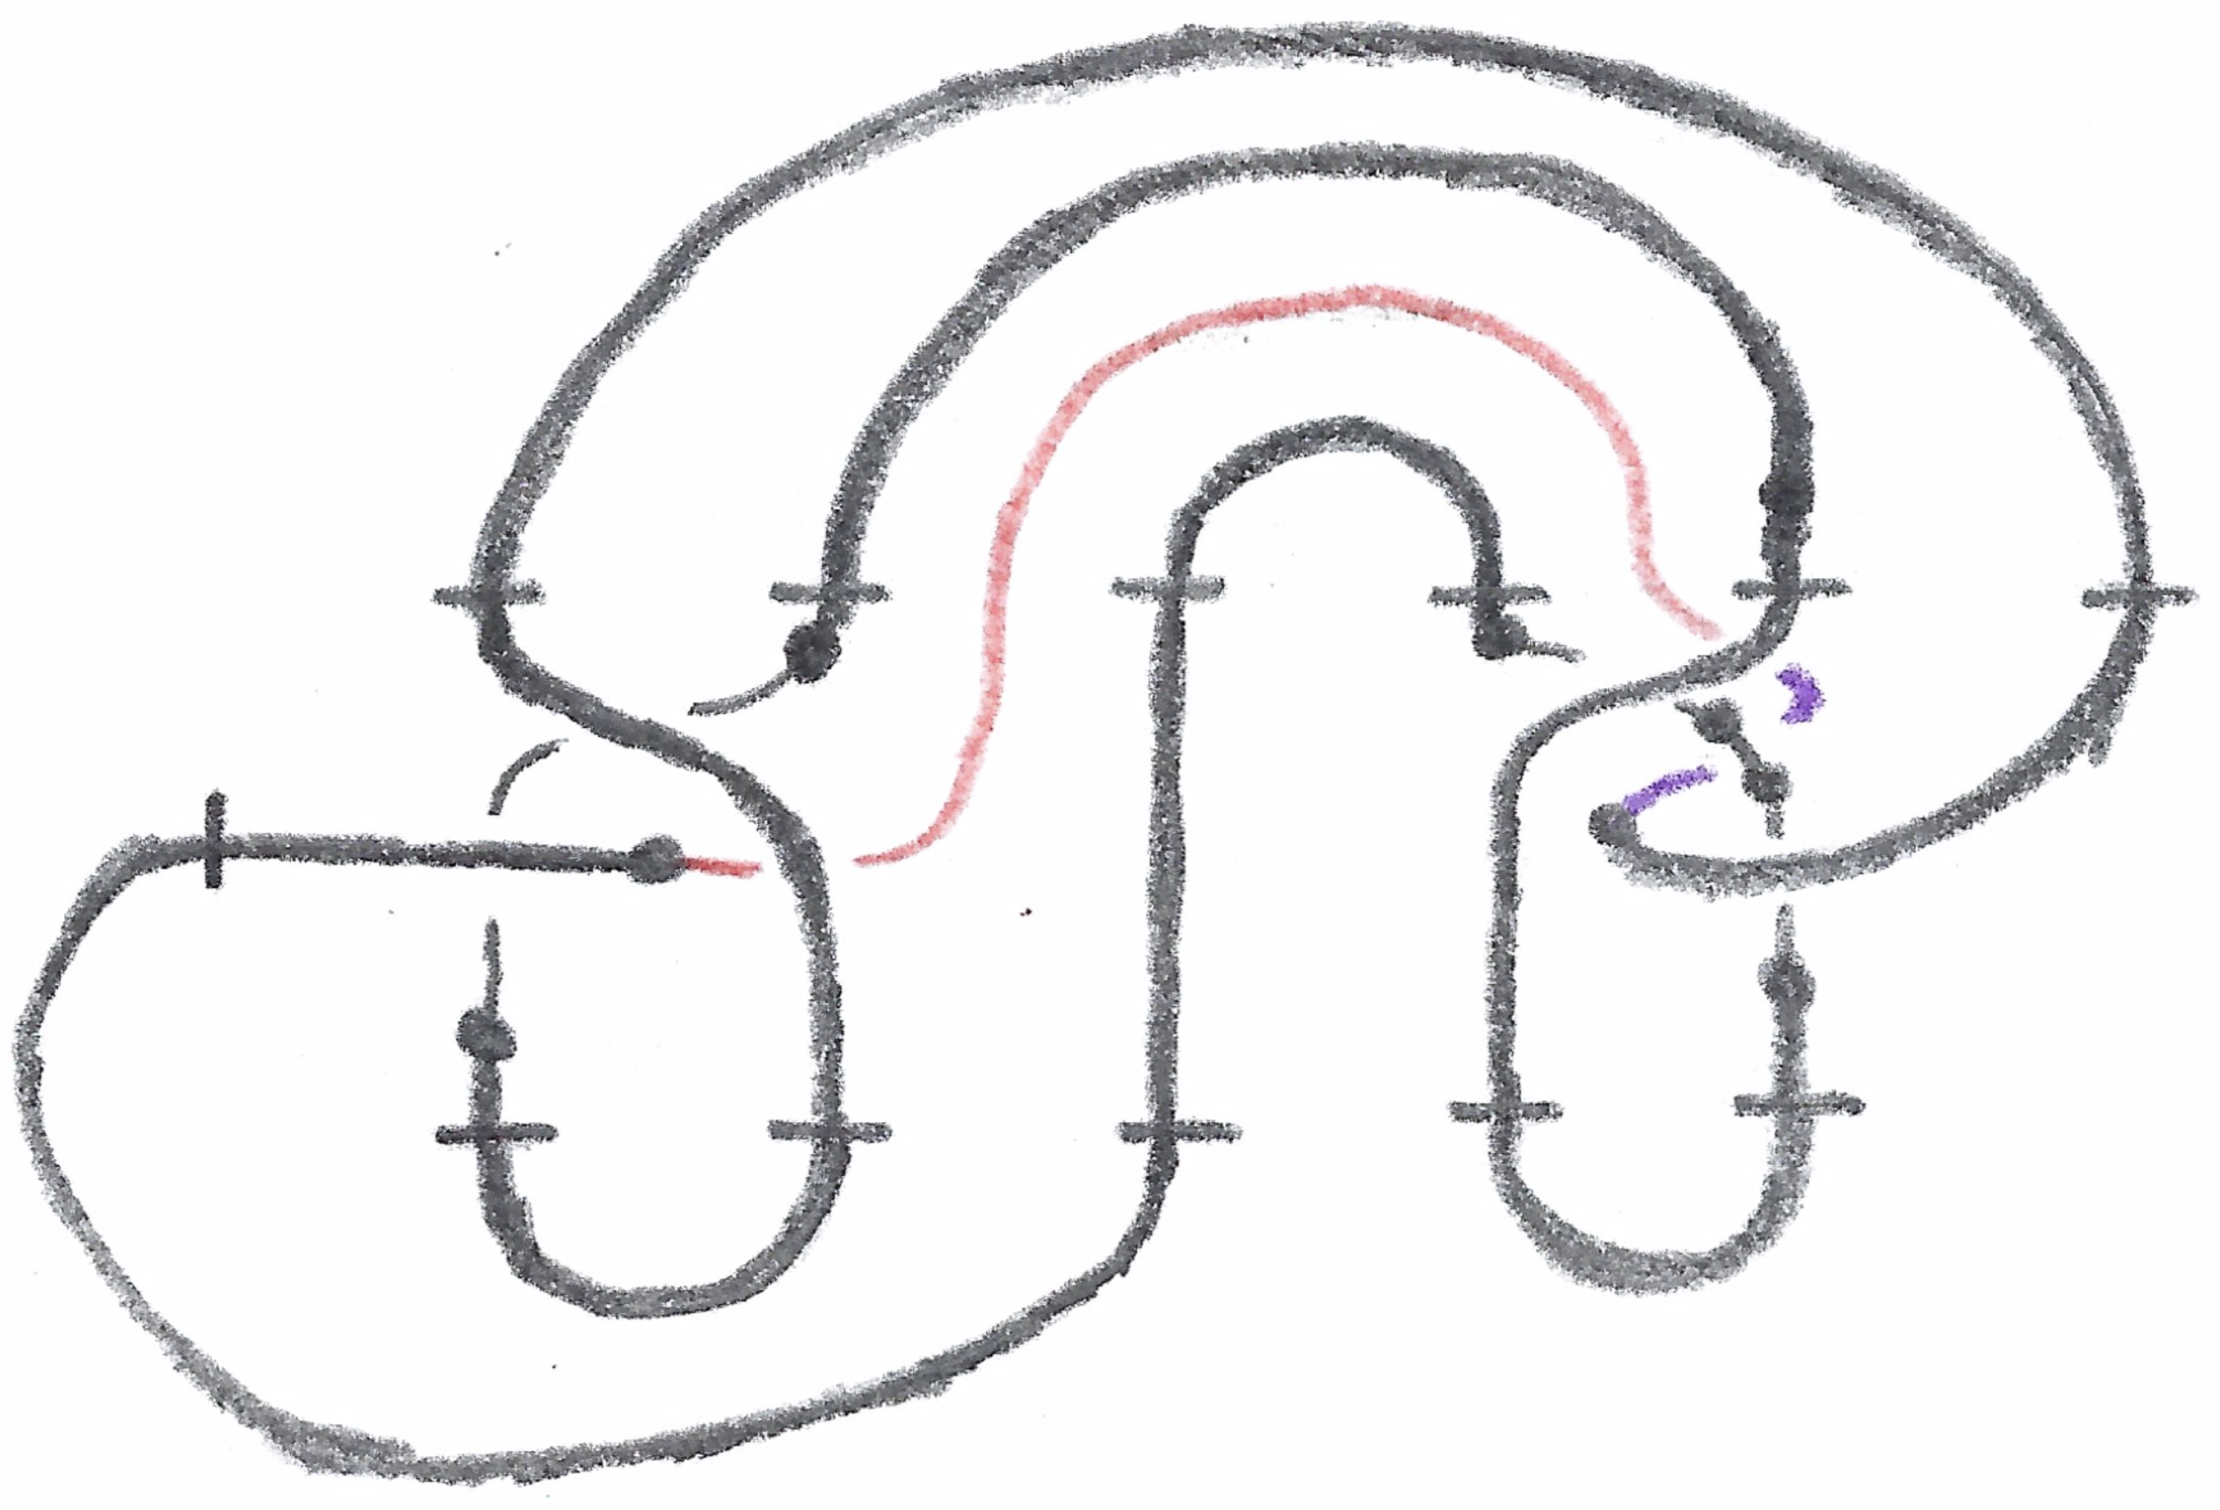
\includegraphics[width=0.8\linewidth]{Blender/ex3-11-2c.png}
                \caption{Bridge number: 4.}
                \label{fig:ex3-11-2c}
            \end{subfigure}
            \par\bigskip
            \begin{subfigure}[b]{0.3\linewidth}
                \centering
                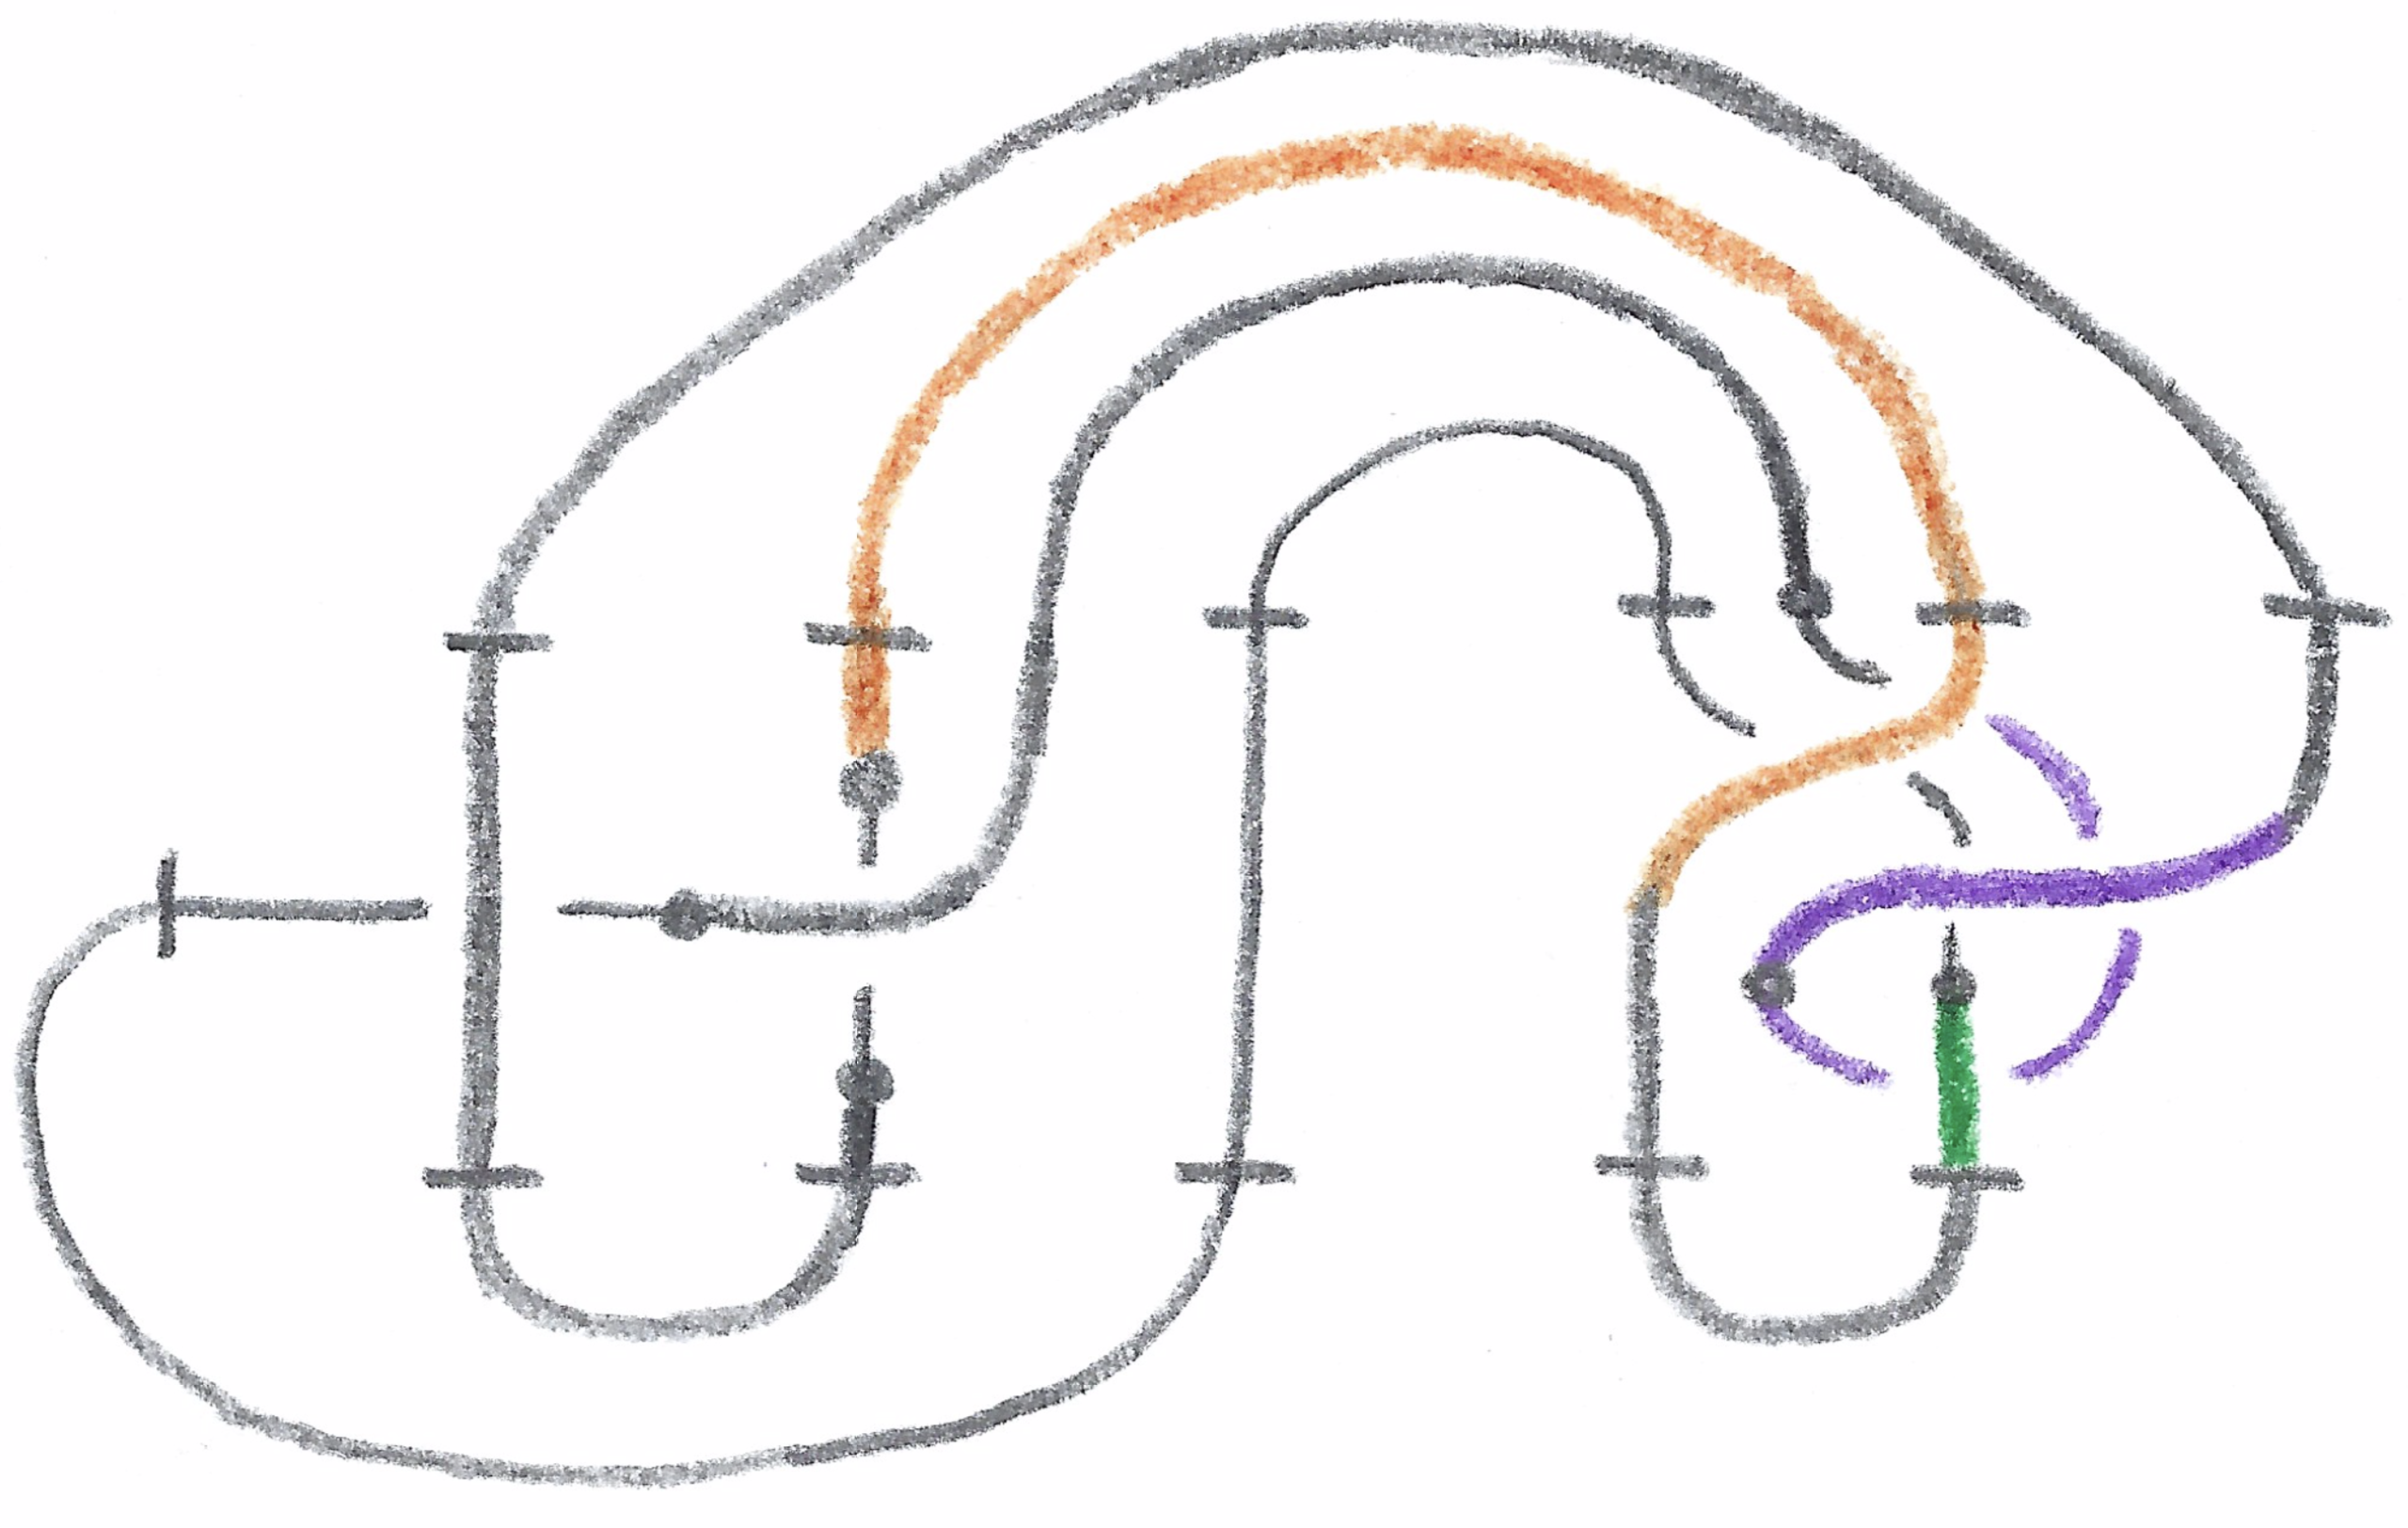
\includegraphics[width=0.8\linewidth]{Blender/ex3-11-2d.png}
                \caption{Bridge number: 3.}
                \label{fig:ex3-11-2d}
            \end{subfigure}
            \begin{subfigure}[b]{0.6\linewidth}
                \centering
                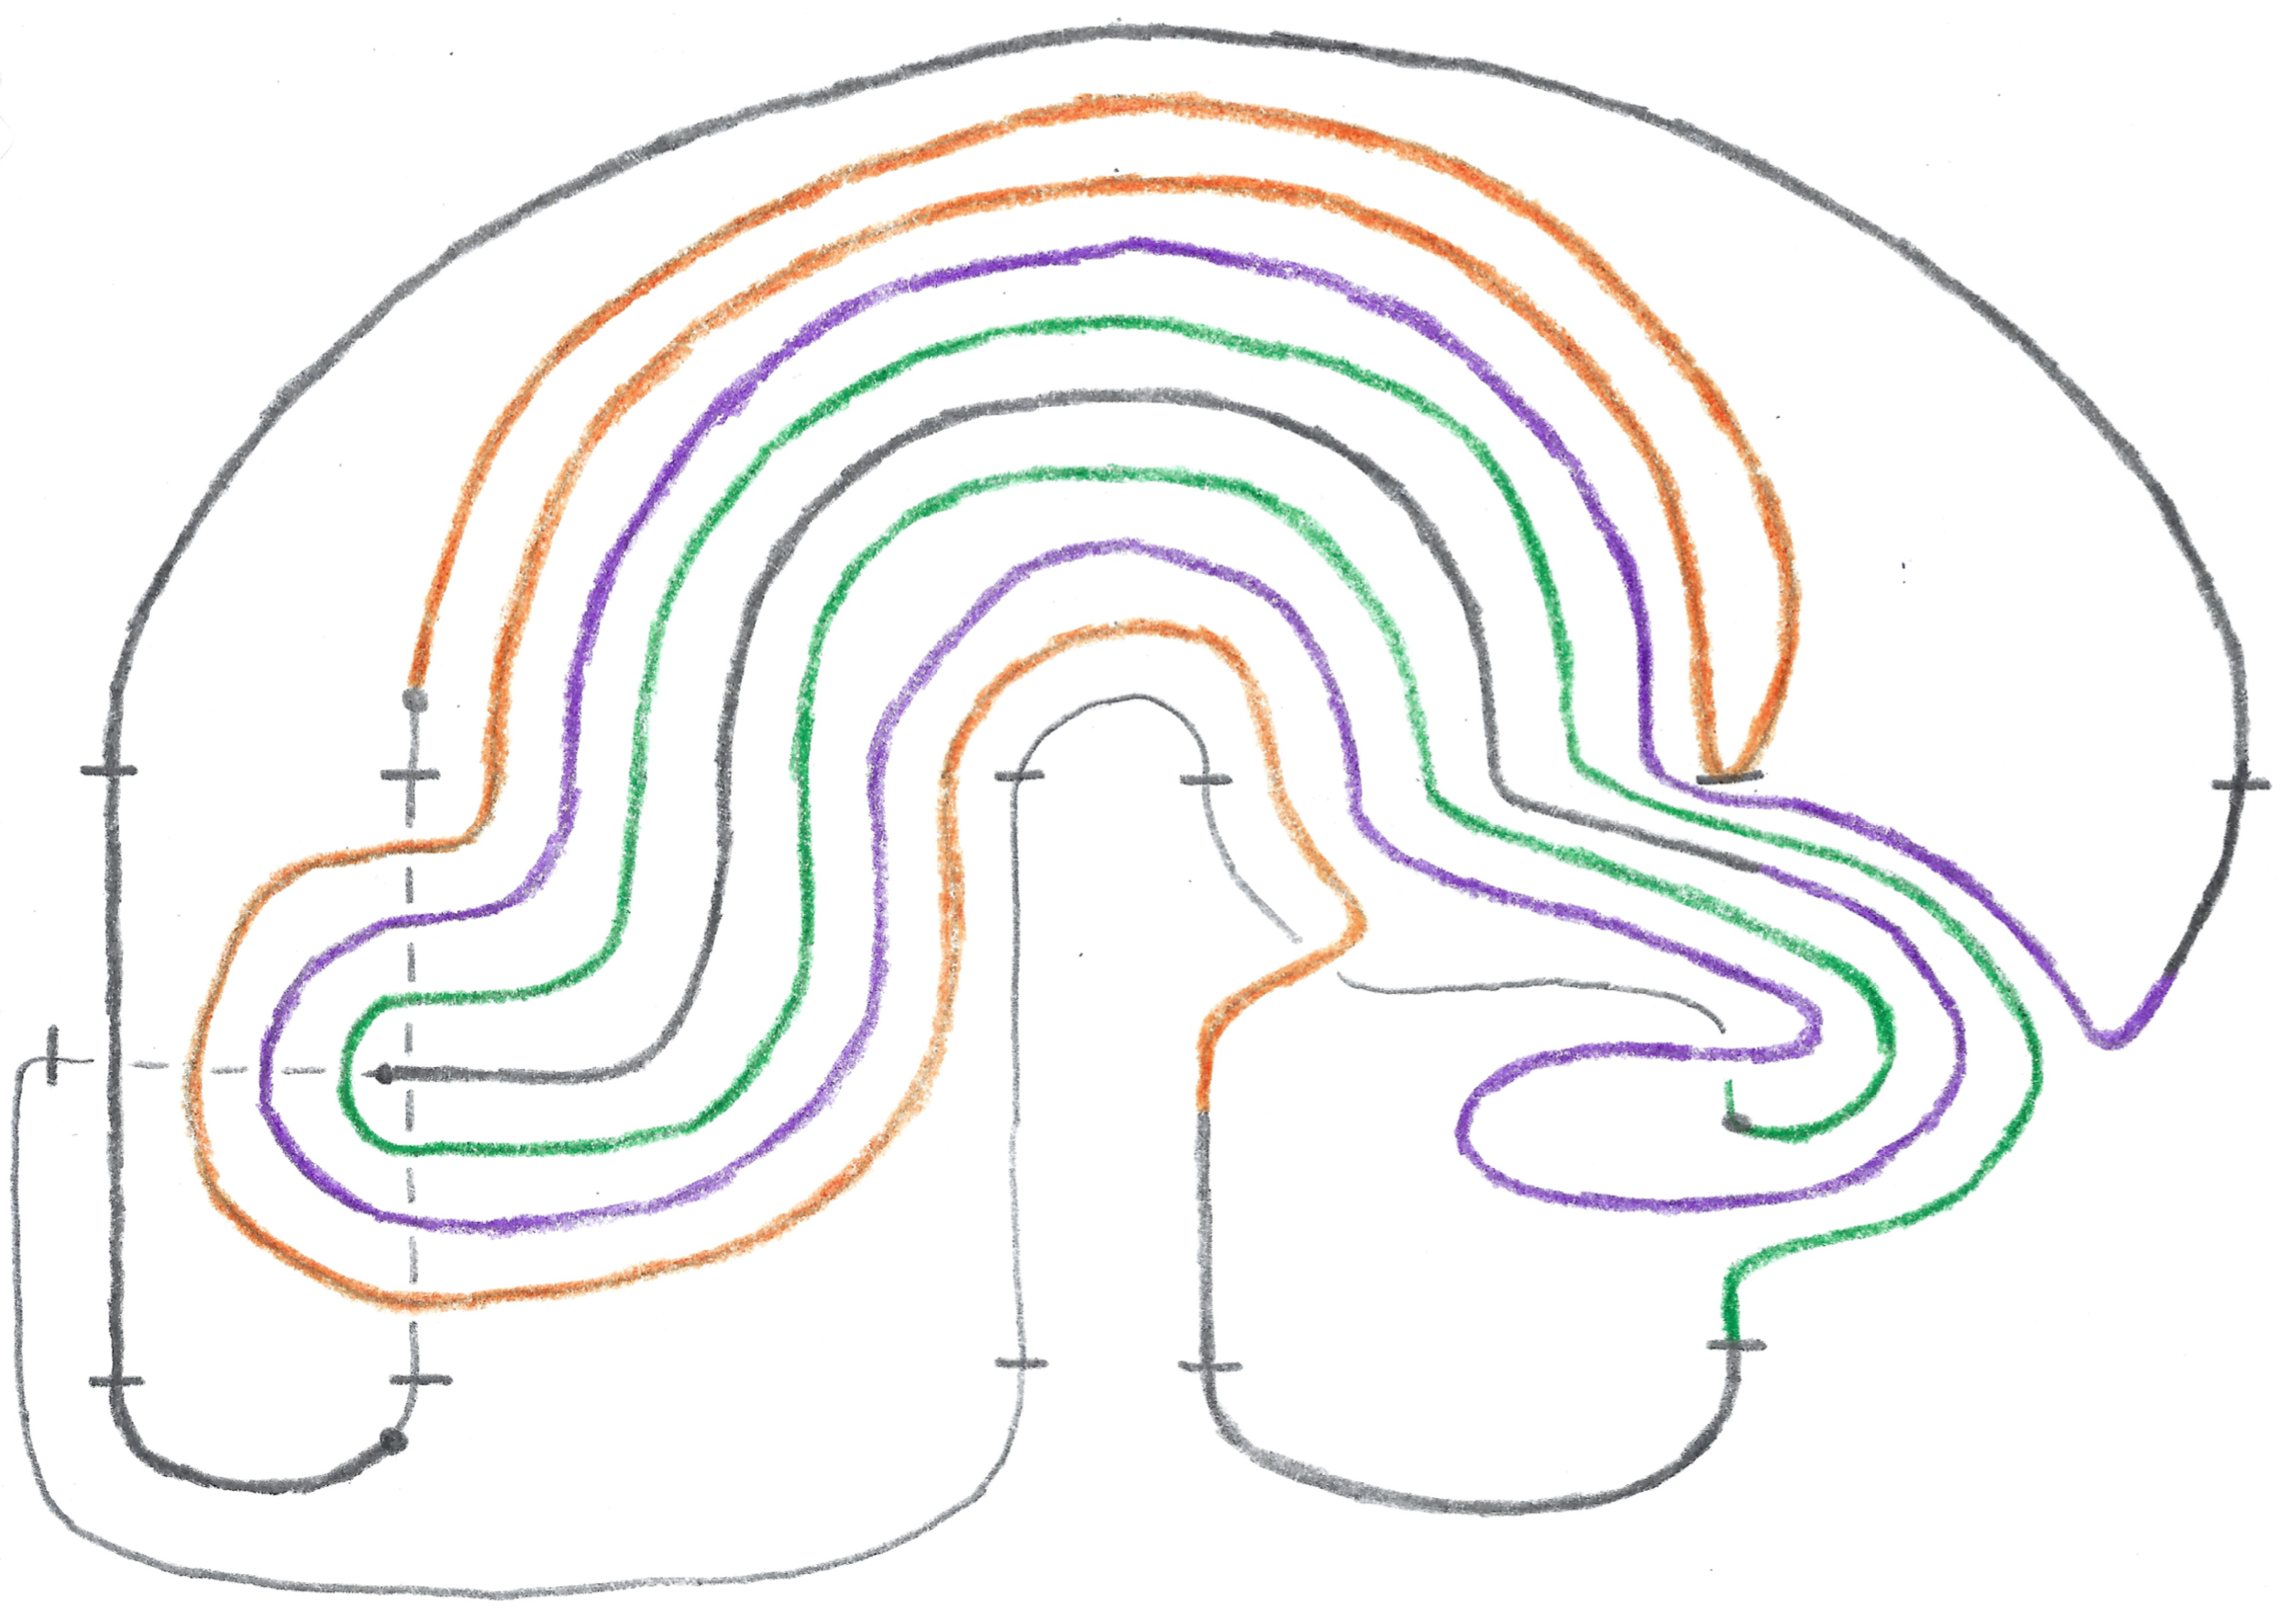
\includegraphics[width=0.8\linewidth]{Blender/ex3-11-2e.png}
                \caption{Bridge number: 2.}
                \label{fig:ex3-11-2e}
            \end{subfigure}
            \par\bigskip
            \begin{subfigure}[b]{0.3\linewidth}
                \centering
                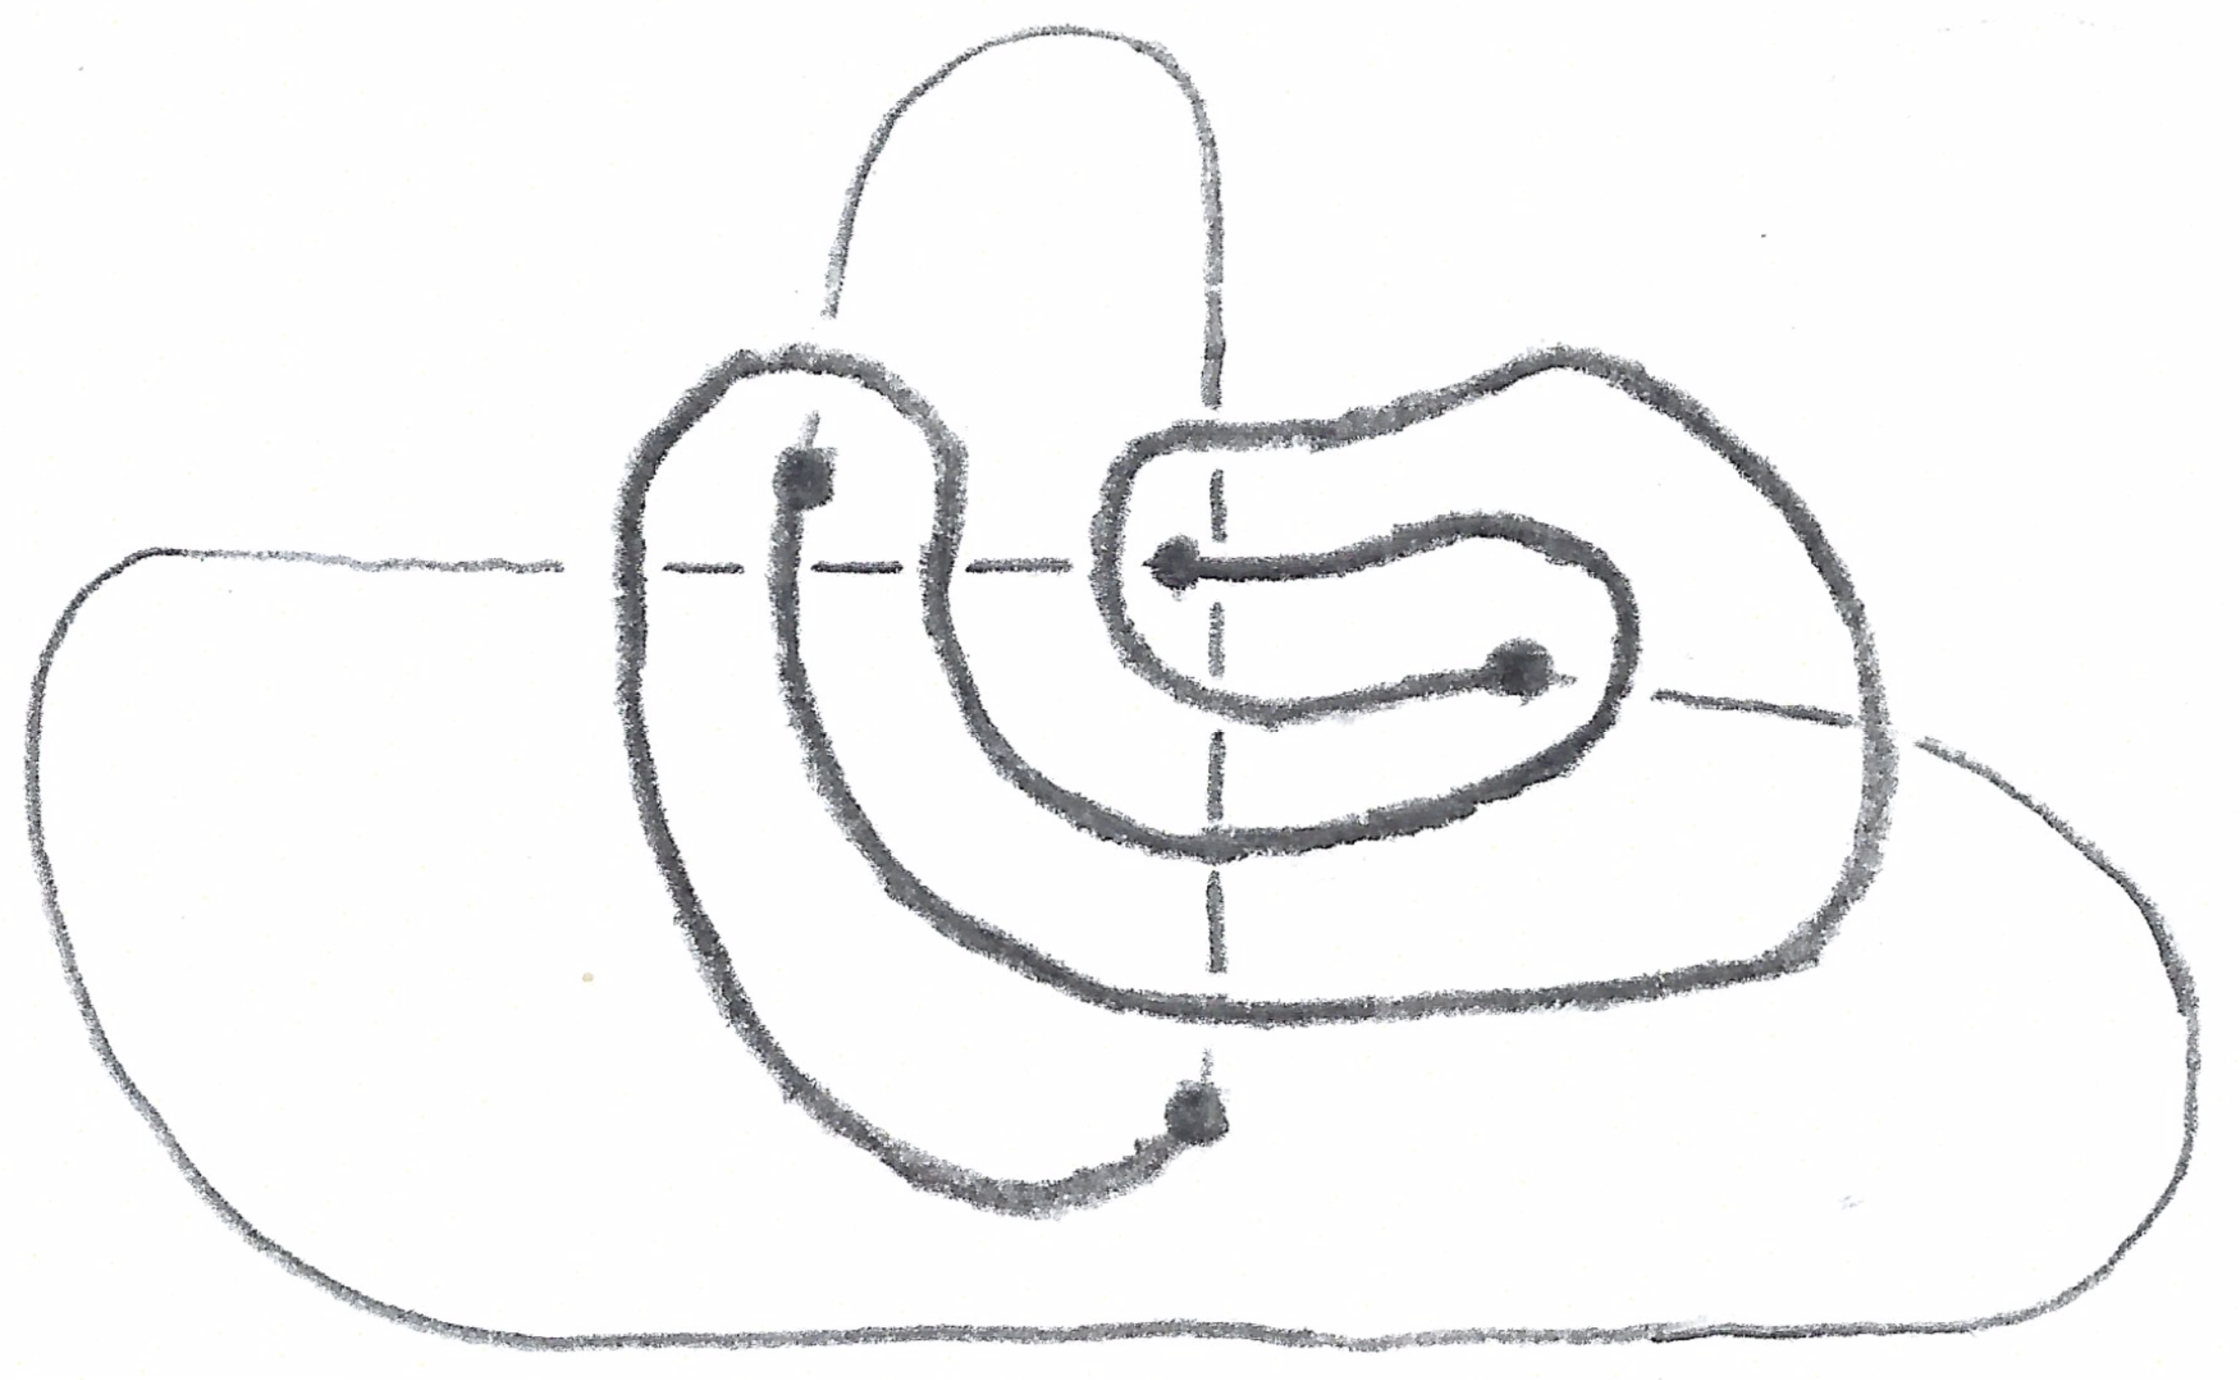
\includegraphics[width=0.8\linewidth]{Blender/ex3-11-2f.png}
                \caption{Bridge number: 2.}
                \label{fig:ex3-11-2f}
            \end{subfigure}
            \caption{Solution to \emph{Exercise 3.11}.}
            \label{fig:ex3-11-2}
        \end{figure}
        \item Note that the following hold for all projections in Figure \ref{fig:ex3-11-2}.
        \begin{itemize}
            \item Dashes, when present, represent the boundaries of the "killzone." They also provide consistent reference points for Figures \ref{fig:ex3-11-2a} through \ref{fig:ex3-11-2e}.
            \item Dots, when present, represent bounds on the overpasses (and, consequently, the underpasses).
            \item Thicker lines represent overpasses. Conversely, thinner lines represent underpasses.
            \item Like-colored strands between sequential projections represent the same strand after Reidemeister moves or planar isotropies (colored for clarity, not for any specific purpose such as tricolorability).
        \end{itemize}
        \item From the previously determined Dowker notation, reconstruct a knot projection. This projection (Figure \ref{fig:ex3-11-2a}) contains the "killzone," a concentrated region where every crossing is displayed in an orderly fashion$^[$\footnote{Note that from here-down, I do not guarantee that this is the fastest or simplest way to generate a projection that displays $b(K)=2$, nor can I assure the reader that my solution is the "simplest" projection (perhaps the one with the fewest crossings). However, I do guarantee that it is correct. I know that it is so because all projections are separated only by Reidemeister moves and planar isotropies, and Figure \ref{fig:ex3-11-2f} visibly has bridge number 2.}$^]$.
        \item Employ two Type I Reidemeister moves followed respectively by Type III Reidemeister moves to eliminate two overpasses. These moves occur on the green and blue strands, independently. They yield a projection with bridge number 3 (Figure \ref{fig:ex3-11-2b}). This projection has several noteworthy properties.
        \begin{itemize}
            \item First, of the three overpasses, two contain 2 crossings while one contains 3 crossings.
            \item Second, of the three underpasses, two contain 2 crossings while one contains 3 crossings.
            \item Third, every overpass crosses at least one of its adjacent underpass.
            \item Because each overpass and underpass has more than one crossing, the bridge number of the projection must increase before it can decrease (one of the overpasses must be split into two [or three]; single overpasses can subsequently be eliminated via "bridging moves").
            \item Because each overpass crosses at least one of its adjacent underpasses, no "bridging moves" can eliminate a bridge from this projection directly$^[$\footnote{I am holding this to be true because I cannot demonstrate otherwise, but I do not know that it is true. I'd actually conjecture that it's false --- it would seem to make sense that some overpass could be eliminated directly from Figure \ref{fig:ex3-11-2b}.}$^]$.
        \end{itemize}
        \item Employ two Type II Reidemeister moves followed by one Type III Reidemeister move to split one of the 2-crossing overpasses into two 1-crossing overpasses. These moves occur on the red-purple strand, which is "slid along" beneath the central overpass. This change will increase the bridge number to 4 and yield Figure \ref{fig:ex3-11-2c}$^[$\footnote{Multiple such moves may suffice here to split a 2-crossing bridge. I chose and followed through this one randomly.}$^]$.
        \item Employ a Type I Reidemeister move followed by a Type III Reidemeister move to eliminate one of the new 1-crossing overpasses. These moves occur on the purple strand. This change will decrease the bridge number back to 3. Additionally, perform the reverse of the actions on the green strand between Figures \ref{fig:ex3-11-2a} and \ref{fig:ex3-11-2b} to "straighten it out." This shift will switch the 1-crossing overpass to an adjacent strand. These changes will yield Figure \ref{fig:ex3-11-2d}. This projection has several noteworthy properties.
        \begin{itemize}
            \item The 1-crossing overpass has underpasses of greater than 1 crossing on both sides.
            \item The 1-crossing overpass passes through a loop, creating a setup similar to the two overpasses eliminated between Figure \ref{fig:ex3-11-2a} and \ref{fig:ex3-11-2b}. However, because of the above, a Type I Reidemeister move followed by a Type III Reidemeister move will not eliminate this overpass --- it would only shift the position of the overpass.
            \item The 1-crossing overpass crosses neither of its adjacent underpasses.
            \item The above is key --- because of it, a succession of 2xType II Reidemeister moves followed by 1xType III Reidemeister moves can combine the 1-crossing overpass with the partially purple overpass.
            \item This set of moves will occur thrice --- once for each crossing of the adjacent underpass.
        \end{itemize}
        \item Three times sequentially, employ two Type II Reidemeister moves followed by one Type III Reidemeister move to (for the first two sets) shift the position of the 1-crossing overpass and then (for the last set) eliminate the 1-crossing overpass. These moves occur on the orange, purple, and green strands, sequentially. They yield a projection with bridge number 2 (Figure \ref{fig:ex3-11-2e}).
        \item Q.E.D.
        \item Figure \ref{fig:ex3-11-2e} is rather visually unpleasant, however. Figure \ref{fig:ex3-11-2f} is the result of one Type I Reidemeister move (on the upper part of the orange strand) and planar isotropies intended purely to "clean up" the projection. It remains indistinct from $5_2$ and displays $b(K)=2$.
    \end{itemize}
    \item \textbf{Two-bridge knots}: Knots that have $b(K)=2$.
    \item If a two-bridge knot is sliced through the projection plane, there will be two \textbf{unknotted untangled} arcs both above and below said plane.
    \item \textbf{Unknotted untangled}: Distinct arcs that have no crossings with each other.
    \item From 2 such unknotted untangled arcs on each side of the projection plane, it is possible to construct all two-bridge knots.
    \begin{itemize}
        \item \dq{The tricky part is that although the strings to each side of the plane
        are individually unknotted, they can twist around each other and themselves}{65}
    \end{itemize}
    \item All two-bridge knots are rational knots and vice versa.
    \item Since the two-bridge knots are a very well understood class of knots, properties that are suspected to hold true for all knots are often first proved to hold true for two-bridge knots.
    \item All two-bridge knots are prime.
    \item The first tabulated three-bridge knot is $8_{10}$.
    \item \emph{Exercise 3.13}: Find a picture of $8_{10}$ that shows that it is at most a three-bridge knot.
    \begin{figure}[h!]
        \centering
        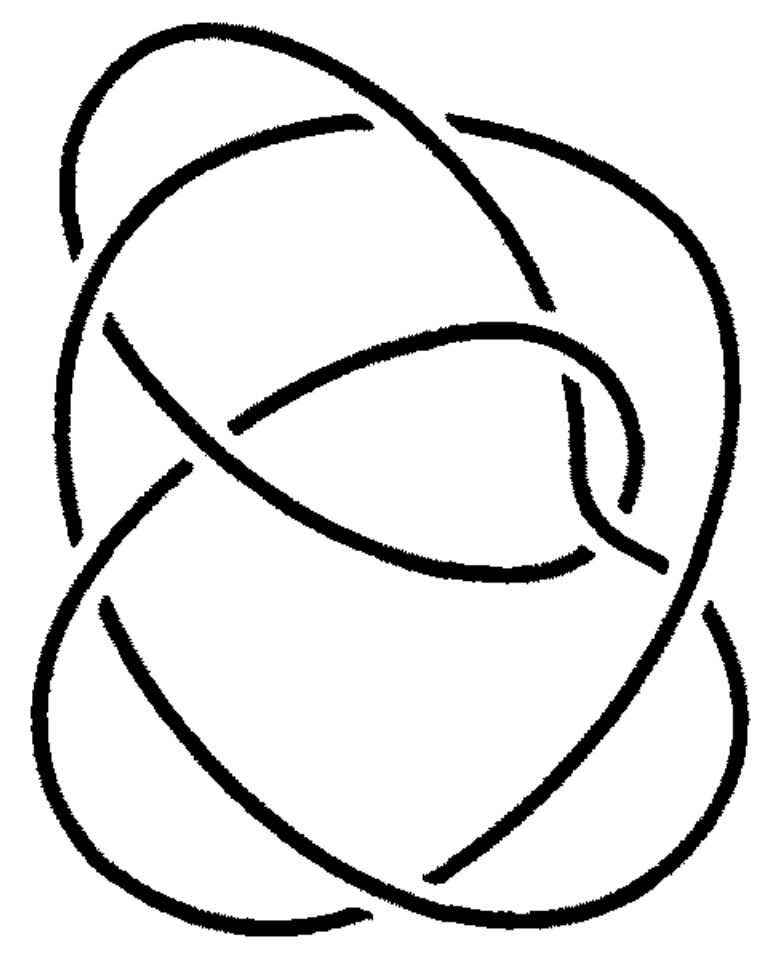
\includegraphics[width=0.12\linewidth]{Blender/ex3-13.png}
        \caption{The knot $8_{10}$.}
        \label{fig:ex3-13}
    \end{figure}
    \begin{itemize}
        \item Find the Dowker notation of $8_{10}$$^[$\footnote{Note that different Dowker notations will lead to different Dowker reconstructions --- some may be easier to manipulate than others. To concentrate the "killzone" in a single (or at least close) to rectangular region, choose Dowker notations with maximum "base strands." Avoid, in the beginning, passing through at a crossing that will soon be passed through again.}$^]$.
        \begin{itemize}
            \item The "maximum" Dowker notation (which, fortunately, is also "ideal") for $8_{10}$ is 12 16 10 14 4 6 2 8
        \end{itemize}
        \item From the previously determined Dowker notation, reconstruct a knot projection.
        \item There are four possible "type I bridging moves"$^[$\footnote{A Type I Reidemeister move performed on an isolated loop followed by a Type III Reidemeister move to translate the new crossing across the "base strand."}$^]$ allowed by this projection. Perform 3 of these to eliminate 3 bridges.
        \begin{itemize}
            \item For the "linked loops," it does matter on which loop the move is performed.
            \item This yields a projection with 2x3-crossing bridges, 2x2-crossing bridges, and 1x1-crossing bridge.
        \end{itemize}
        \item Perform two "type II bridging moves"$^[$\footnote{Two Type II Reidemeister moves performed on the same strand to move it over either side of an adjacent crossing followed by a Type III Reidemeister move to translate the strand over the crossing followed by two Type II Reidemeister moves for simplification purposes.}$^]$ to eliminate the 1-crossing bridge.
        \item Perform four "type II bridging moves" to eliminate a 2-crossing bridge.
        \begin{figure}[h!]
            \centering
            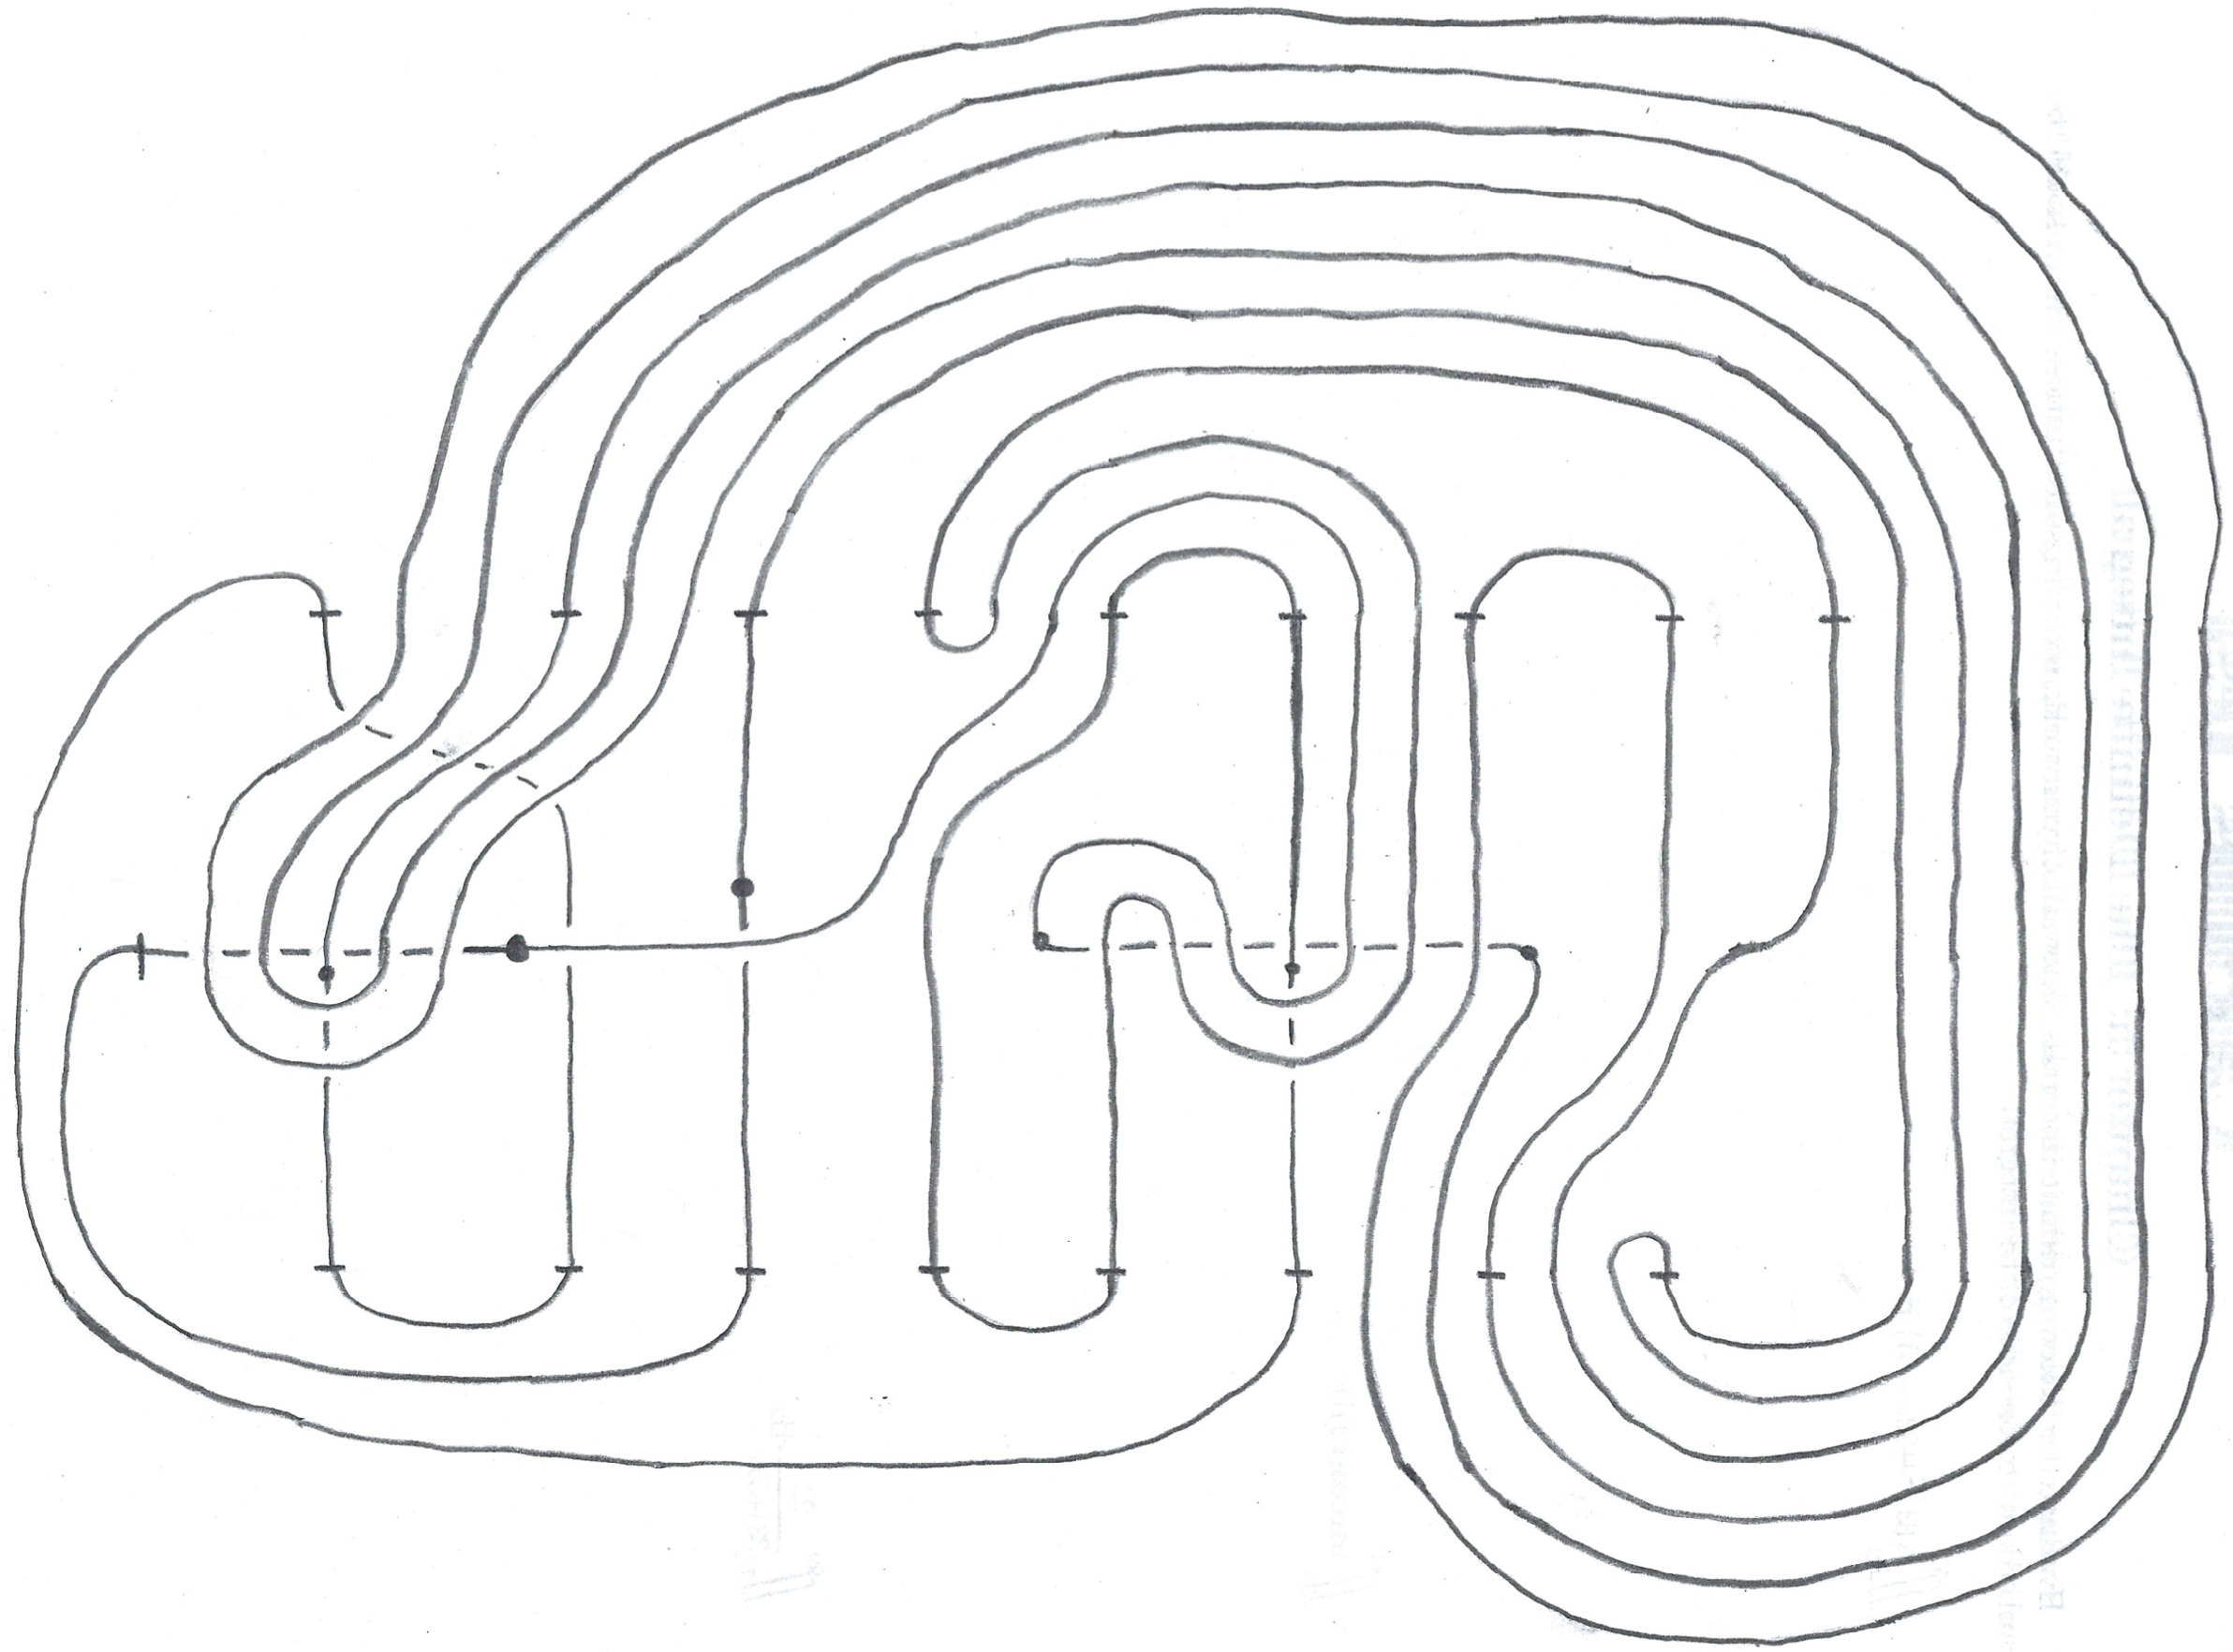
\includegraphics[width=0.9\linewidth]{Blender/ex3-13-2.png}
            \caption{Solution to \emph{Exercise 3.13}.}
            \label{fig:ex3-13-2}
        \end{figure}
        \item Q.E.D. --- see Figure \ref{fig:ex3-13-2} for the final projection$^[$\footnote{Note that this figure is drawn with the same rules used in Exercise 3.11, i.e. the original "killzone" is marked as well as the start and end of each bridge. Each "bridging move" has been carried out without simplification, so some thought should be able to reveal the connection between the original Dowker reconstruction (not pictured) and this projection.}$^]$.
    \end{itemize}
    \item \dq{In 1954, a German mathematician named H. Shubert proved that $b(K_1\#K_2)=b(K_1)+b(K_2)-1$}{67}
    \item \emph{Exercise 3.14}: Explain how Shubert's result implies that rational knots are all prime.
    \begin{itemize}
        \item To be distinct from the unknot, a knot must have $b(K)\geq 2$, as proven in \emph{Exercise 3.10}.
        \item By Shubert's theorem, above, and the above fact, any composition of two nontrivial knots must have $b(K)\geq 3$ (at least $2+2-1=3$).
        \item Since any knot with $b(K)\geq 3$ is not rational and all composite knots have $b(K)\geq 3$, all rational knots (those with $b(K)=2$) must be noncomposite, or prime.
    \end{itemize}
\end{itemize}


\subsection{Crossing Number}
\begin{itemize}
    \item \textbf{Crossing number}: \dq{The least number of crossings that occur in any projection of the knot}{67} \emph{Also known as} $\mathbf{c(K)}$.
    \item To find the crossing number of a knot, first find a projection of the knot. Count the crossings, $n$. At this point, it is clear that $c(K)\leq n$.
    \begin{itemize}
        \item If all knots with fewer crossing than $n$ are known and $K$ is distinct from all of those knots, then $c(K)=n$.
        \item Otherwise, reduce the knot to its minimal projection.
    \end{itemize}
    \item Proving that a knot is distinct from every knot of fewer crossings is very difficult and requires knot polynomials (see Section \ref{sse:polynomials}).
    \item Determining $c(K)$ is generally very difficult (knots are currently only tabulated up to 13 crossings).
    \item \textbf{Reduced}: A projection of a knot with no easily removed crossings.
    \begin{itemize}
        \item All "easily removed" crossings in alternating knots are shown in Figure \ref{fig:easilyremoved}.
    \end{itemize}
    \begin{figure}[h!]
        \centering
        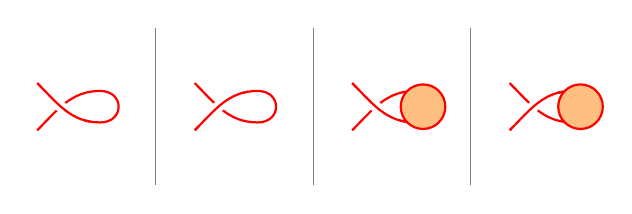
\begin{tikzpicture}
            \foreach \x in {-2,0,2} {
                \draw[help lines] (\x,-1) -- (\x,1);
            }
            \begin{knot}[
                clip width=5,
                consider self intersections,
                xshift=-3cm
            ]
                \strand[red,thick] (-0.5,0.3)
                    to [out=-45,in=180] (0.3,-0.2)
                    to [out=0,in=0,looseness=2] (0.3,0.2)
                    to [out=180,in=45]   (-0.5,-0.3)
                ;
            \end{knot}
            \begin{knot}[
                clip width=5,
                consider self intersections,
                xshift=-1cm,
                flip crossing=1
            ]
                \strand[red,thick] (-0.5,0.3)
                    to [out=-45,in=180] (0.3,-0.2)
                    to [out=0,in=0,looseness=2] (0.3,0.2)
                    to [out=180,in=45]   (-0.5,-0.3)
                ;
            \end{knot}
            \begin{knot}[
                clip width=5,
                consider self intersections,
                xshift=1cm
            ]
                \strand[red,thick] (-0.5,0.3)
                    to [out=-45,in=180] (0.3,-0.2)
                    to [out=0,in=0,looseness=2] (0.3,0.2)
                    to [out=180,in=45]   (-0.5,-0.3)
                ;
            \end{knot}
            \begin{knot}[
                clip width=5,
                consider self intersections,
                xshift=3cm,
                flip crossing=1
            ]
                \strand[red,thick] (-0.5,0.3)
                    to [out=-45,in=180] (0.3,-0.2)
                    to [out=0,in=0,looseness=2] (0.3,0.2)
                    to [out=180,in=45]   (-0.5,-0.3)
                ;
            \end{knot}
            \node at (1.4,0) [circle,inner sep=2mm,draw=red,thick,fill=orange!50]{};
            \node at (3.4,0) [circle,inner sep=2mm,draw=red,thick,fill=orange!50]{};
        \end{tikzpicture}
        \caption{Easily removed crossings in an alternating knot projection.}
        \label{fig:easilyremoved}
    \end{figure}
    \item However, in 1986, Lou Kauffman, Kunio Murasugi, and Morwen Thistlethwaite all independently proved that \dq{an alternating knot in a reduced alternating projection of $n$ crossings has crossing number $n$}{68}.
    \begin{itemize}
        \item They utilized the Jones polynomial (see Section \ref{sse:polynomials}).
        \item Because we can visually tell whether or not a projection is reduced (and reduce it if it's not), we can determine $c(K)$ for any alternating knot.
    \end{itemize}
    \item It is still unknown whether or not $c(K_1\#K_2)=c(K_1)+c(K_2)$.
    \begin{itemize}
        \item However, Kaufman, Murasugi, and Thistlethwaite's result proves that the above holds when $K_1\#K_2$ is alternating.
    \end{itemize}
    \item \emph{Exercise 3.15}: Show that if $K_1$ and $K_2$ are alternating, then so is $K_1\#K_2$. Hence, $c(K_1\#K_2)=c(K_1)+c(K_2)$ holds when $K_1$ and $K_2$ are alternating even if $K_1\#K_2$ does not appear alternating.
    \begin{figure}[h!]
        \centering
        \begin{subfigure}[b]{0.4\linewidth}
            \centering
            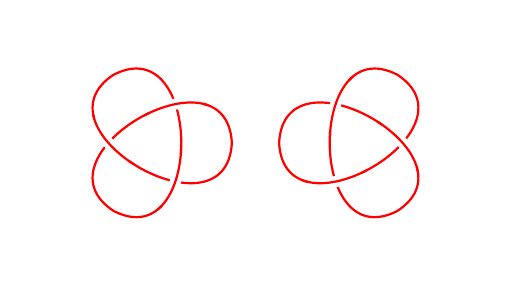
\begin{tikzpicture}
                \begin{knot}[
                    clip width=5,
                    consider self intersections,
                    xshift=-1.3cm
                ]
                    \strand[red,thick] (120:1)
                        \foreach \x in {1,2,3} {
                            to [bend left=117,looseness=1.9] ({120+120*\x}:1)
                        }
                    ;
                    \flipcrossings{1,3}
                \end{knot}
                \begin{knot}[
                    clip width=5,
                    consider self intersections,
                    xshift=1.3cm
                ]
                    \strand[red,thick] (60:1)
                        \foreach \x in {1,2,3} {
                            to [bend left=117,looseness=1.9] ({60+120*\x}:1)
                        }
                    ;
                    \flipcrossings{1,3}
                \end{knot}
            \end{tikzpicture}
            \vspace{-0.4cm}
            \caption{$3_1$ and $3_1$.}
            \label{fig:alternatingcomposa}
        \end{subfigure}
        \begin{subfigure}[b]{0.3\linewidth}
            \centering
            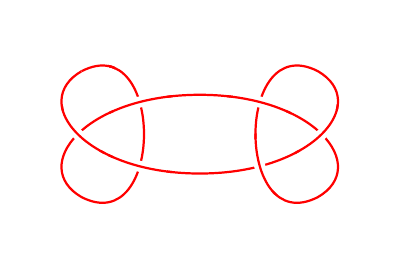
\begin{tikzpicture}
                \def\x{1}
                \def\y{1.5}
                \begin{knot}[
                    clip width=5,
                    consider self intersections,
                    ignore endpoint intersections=false
                ]
                    \strand[red,thick] (-\y,0.8)
                        to [bend left=117,looseness=1.9] (-\y,-0.8)
                        to [out=150,in=180,out looseness=\x,in looseness=1.9] (0,0.5)
                        to [out=0,in=30,out looseness=1.9,in looseness=\x] (\y,-0.8)
                        to [bend left=117,looseness=1.9] (\y,0.8)
                        to [out=-30,in=0,out looseness=\x,in looseness=1.9] (0,-0.5)
                        to [out=180,in=-150,out looseness=1.9, in looseness=\x] cycle
                    ;
                    \flipcrossings{1,4,5,7}
                \end{knot}
            \end{tikzpicture}
            \vspace{-0.4cm}
            \caption{$3_1\#3_1$.}
            \label{fig:alternatingcomposb}
        \end{subfigure}
        \begin{subfigure}[b]{0.4\linewidth}
            \centering
            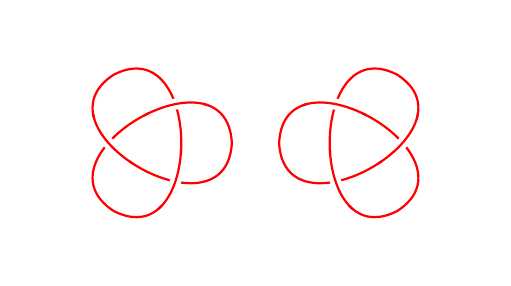
\begin{tikzpicture}
                \begin{knot}[
                    clip width=5,
                    consider self intersections,
                    xshift=-1.3cm
                ]
                    \strand[red,thick] (120:1)
                        \foreach \x in {1,2,3} {
                            to [bend left=117,looseness=1.9] ({120+120*\x}:1)
                        }
                    ;
                    \flipcrossings{1,3}
                \end{knot}
                \begin{knot}[
                    clip width=5,
                    consider self intersections,
                    xshift=1.3cm
                ]
                    \strand[red,thick] (60:1)
                        \foreach \x in {1,2,3} {
                            to [bend left=117,looseness=1.9] ({60+120*\x}:1)
                        }
                    ;
                    \flipcrossings{2}
                \end{knot}
            \end{tikzpicture}
            \vspace{-0.4cm}
            \caption{$3_1$ and $3_1$'s mirror image.}
            \label{fig:alternatingcomposc}
        \end{subfigure}
        \begin{subfigure}[b]{0.3\linewidth}
            \centering
            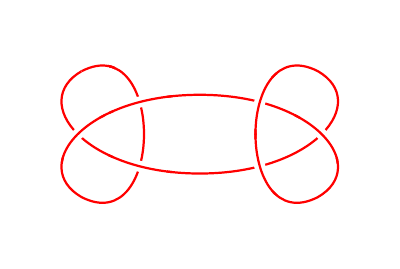
\begin{tikzpicture}
                \def\x{1}
                \def\y{1.5}
                \begin{knot}[
                    clip width=5,
                    consider self intersections,
                    ignore endpoint intersections=false
                ]
                    \strand[red,thick] (-\y,0.8)
                        to [bend left=117,looseness=1.9] (-\y,-0.8)
                        to [out=150,in=180,out looseness=\x,in looseness=1.9] (0,0.5)
                        to [out=0,in=30,out looseness=1.9,in looseness=\x] (\y,-0.8)
                        to [bend left=117,looseness=1.9] (\y,0.8)
                        to [out=-30,in=0,out looseness=\x,in looseness=1.9] (0,-0.5)
                        to [out=180,in=-150,out looseness=1.9, in looseness=\x] cycle
                    ;
                    \flipcrossings{1,4,6}
                \end{knot}
            \end{tikzpicture}
            \vspace{-0.4cm}
            \caption{$3_1\#3_1$ nonalternating.}
            \label{fig:alternatingcomposd}
        \end{subfigure}
        \begin{subfigure}[b]{0.3\linewidth}
            \centering
            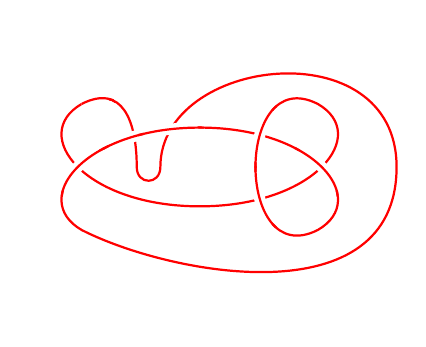
\begin{tikzpicture}
                \def\x{1}
                \def\y{1.5}
                \begin{knot}[
                    clip width=5,
                    consider self intersections,
                    ignore endpoint intersections=false
                ]
                    \strand[red,thick] (-\y,0.8)
                        to [out=27,in=90,looseness=1.4] (-0.8,0)
                        to [out=-90,in=-90,looseness=2] (-0.5,0)
                        to [out=90,in=90,out looseness=1.2,in looseness=1.5] (2.5,0)
                        to [out=-90,in=-27,out looseness=1.2,in looseness=0.8] (-\y,-0.8)
                        to [out=150,in=180,out looseness=\x,in looseness=1.9] (0,0.5)
                        to [out=0,in=30,out looseness=1.9,in looseness=\x] (\y,-0.8)
                        to [bend left=117,looseness=1.9] (\y,0.8)
                        to [out=-30,in=0,out looseness=\x,in looseness=1.9] (0,-0.5)
                        to [out=180,in=-150,out looseness=1.9, in looseness=\x] cycle
                    ;
                    \flipcrossings{1,4,6}
                \end{knot}
            \end{tikzpicture}
            \vspace{-0.4cm}
            \caption{$3_1\#3_1$ made alternating.}
            \label{fig:alternatingcompose}
        \end{subfigure}
        \caption{Drawing an alternating projection of $K_1\#K_2$ where $K_1$ and $K_2$ are alternating.}
        \label{fig:alternatingcompos}
    \end{figure}
    \begin{itemize}
        \item When composing alternating knots, there are two cases, as exemplified by Figure \ref{fig:alternatingcomposa} and \ref{fig:alternatingcomposc}, respectively.
        \begin{itemize}
            \item Case 1: the composite knot will be in an alternating projection.
            \item Case 2: the composite knot will not be in an alternating projection.
        \end{itemize}
        \item For Case 1, the theorem evidently holds. See Figure \ref{fig:alternatingcomposb}
        \item For Case 2, first consider the definition of an alternating knot (see Section \ref{sss:Introduction}), which states that an alternating knot need only have \underline{a} projection that is alternating, i.e., \underline{every} projection need not be alternating.
        \item Therefore, if we can prove that every nonalternating projection obtained through a composition has an alternating equivalent, the theorem will be true. To begin, consider several subcases to determine a pattern in the nonalternation.
        \begin{itemize}
            \item Because $K_1$ and $K_2$ are both alternating, any arc being removed (to compose the two) will necessarily be on an understrand becoming an overstrand or vice versa.
            \item Therefore, if we leave $K_1$ to enter $K_2$ from an understrand, we will return into $K_1$ to meet an overstrand and vice versa. The same holds for $K_2$.
            \item Case A: Leaving from an understrand in $K_1$, enter $K_2$ on an understrand. The next crossing (continuing through $K_2$) will be an overstrand, and then an understrand, \dots\ Eventually, by the above, we will return from $K_2$ on an overstrand into an overstrand on $K_1$. The next crossing (continuing through $K_1$) will be an understrand, and then an overstrand, \dots\ Eventually, we will return to where we started.
            \item Case B: Leaving from an overstrand in $K_1$, enter $K_2$ on an overstrand. The next crossing (continuing through $K_2$) will be an understrand, and then an overstrand, \dots\ Eventually, by the above, we will return from $K_2$ on an understrand into an understrand on $K_1$. The next crossing (continuing through $K_1$) will be an overstrand, and then an understrand, \dots\ Eventually, we will return to where we started.
        \end{itemize}
        \item In both Cases A and B, the only moments of nonalternation are two consecutive underpasses (or overpasses) followed by a factor knot followed by two consecutive overpasses (or underpasses). Notice this pattern in Figure \ref{fig:alternatingcomposd}.
        \item Thus, "slide" one strand of a factor knot over the other knot to eliminate the nonalternation, as in Figure \ref{fig:alternatingcompose}.
        \item Q.E.D.
    \end{itemize}
\end{itemize}
\newpage



\section{Surfaces and Knots}
\subsection{Surfaces without Boundary}
\begin{itemize}
    \item \textbf{Surface}: The two-dimensional exterior of a three-dimensional object with volume.
    \item \textbf{Torus}: \dq{The surface of a donut}{71} \emph{Plural is} \textbf{tori}.
    \item \dq{At any point on a surface, there is a small region on the surface surrounding and containing the point that looks like a disk}{72}
    \begin{itemize}
        \item The disk may be deformed (curved), but it must still be a disk.
        \item Objects that are not surfaces have points with nondisk "neighborhoods" around them.
    \end{itemize}
    \item Surfaces can also be called \textbf{two-manifolds}.
    \item \textbf{Two-manifold}: \dq{Any object such that every point in that object has a neighborhood in the object that is a (possibly nonflat) disk}{73}
    \item \emph{Exercise 4.1}: Based on the definition for two-manifolds, decide what the definition should be for a one-manifold. Find two different one manifolds.
    \begin{itemize}
        \begin{figure}[h!]
            \centering
            \begin{subfigure}[b]{0.2\linewidth}
                \centering
                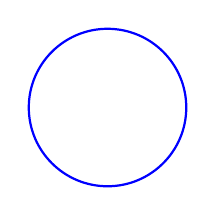
\begin{tikzpicture}
                    \draw [blue,thick] circle (1cm);
                \end{tikzpicture}
                \caption{A circle.}
                \label{fig:1manifoldsa}
            \end{subfigure}
            \begin{subfigure}[b]{0.2\linewidth}
                \centering
                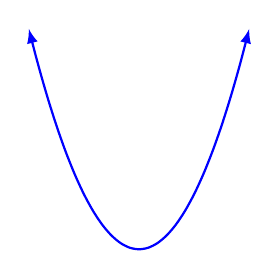
\begin{tikzpicture}[
                    scale=0.7
                ]
                    \draw [blue,thick,latex-latex] plot[smooth,domain=-2:2] (\x,\x*\x);
                    %could use parabola instead of plot
                \end{tikzpicture}
                \caption{A parabola.}
                \label{fig:1manifoldsb}
            \end{subfigure}
            \caption{Two one-manifolds.}
            \label{fig:1manifolds}
        \end{figure}
        \item Any object such that every point in that object has a neighborhood in the object that is a (possibly not straight) line.
    \end{itemize}
    \item See Section \ref{sse:topology} for info on three-manifolds.
    \item Think of surfaces as being made of rubber. In Figure \ref{fig:cubesphere}, the deformation is an \textbf{isotropy} and the left and right surfaces are \textbf{isotropic surfaces}.
    \item \textbf{Isotropy}: A continuous deformation of a surface in space; a rubber deformation.
    \item \textbf{Isotropic surfaces}: Two surfaces in space that are equivalent under an isotropy.
    \item Surfaces that are not isotropic cannot be deformed into one another without some cutting and pasting!$^[$\footnote{Identify surfaces by the number of holes in them?}$^]$
    \begin{figure}[h!]
        \centering
        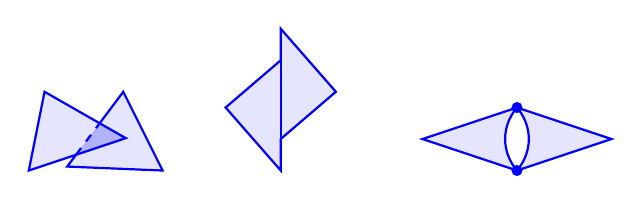
\begin{tikzpicture}
            \colorlet{bly}{blue!10}
            \begin{scope}[
                xshift=-3cm
            ]
                \fill [bly] (0.4,0.2) -- (-0.2,0) -- (0,1) -- (0.7,0.6);
                \fill [bly] (0.7,0.6) -- (1,1) -- (1.5,0) -- (0.2875,0.05) -- (0.4,0.2);
                \fill [bly!300] (0.4,0.2) -- (1.032,0.411) -- (0.7,0.6);
                
                \draw [blue,thick] (0.4,0.2) -- (-0.2,0) -- (0,1) -- (0.7,0.6) -- (1,1) -- (1.5,0) -- (0.2875,0.05) -- cycle;
                \draw [blue,thick,dashed] (0.4,0.2) -- (0.7,0.6);
                \draw [blue,thick] (0.4,0.2) -- (1.032,0.411) -- (0.7,0.6);
            \end{scope}
            \filldraw [draw=blue,fill=bly,thick] (0,0.4) -- (0,0) -- (-0.7,0.8) -- (0,1.4) -- (0,1.8) -- (0.7,1) -- cycle;
            \draw [blue,thick] (0,0.4) -- (0,1.4);
            \begin{scope}[
                xshift=3cm
            ]
                \filldraw [draw=blue,fill=bly,thick] (0,0) -- (-1.2,0.4) -- (0,0.8) to [out=-130,in=130] cycle;
                \filldraw [draw=blue,fill=bly,thick] (0,0) -- (1.2,0.4) -- (0,0.8) to [out=-50,in=50] cycle;
                \foreach \y in {0,0.8} {
                    \fill [blue] (0,\y) circle (2pt);
                }
            \end{scope}
        \end{tikzpicture}
        \caption{Triangles cannot intersect like this.}
        \label{fig:triangleintersects}
    \end{figure}
    \item \textbf{Triangulation}: A division of a surface into deformable triangles.
    \begin{itemize}
        \item Think of a triangle as a disk \dq{with a boundary made up of three edges connecting three vertices}{75}
        \item The triangles must \dq{fit together nicely along their edges so that they cover the entire surface}{74} See Figure \ref{fig:triangleintersects} for a visualization of ways that triangles cannot fit together.
        \item Given a triangulation of a surface, the triangles can be separated and we can keep track of the original surface by labeling edges and putting arrows on them.
    \end{itemize}
    \begin{figure}[h!]
        \centering
        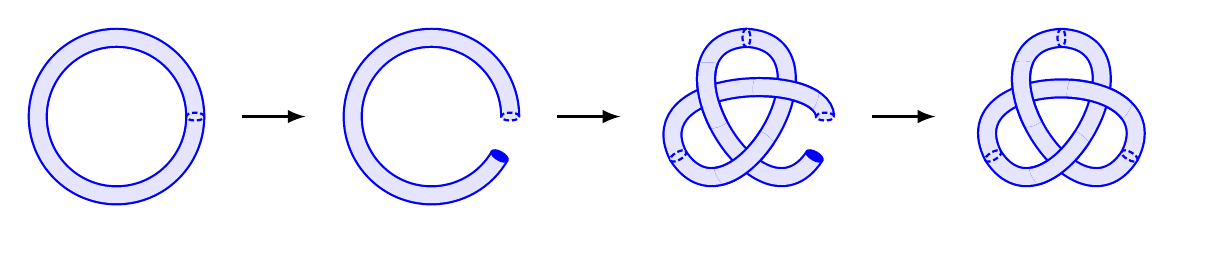
\begin{tikzpicture}[
            arrow/.style={very thick,-latex,black}
        ]
            \colorlet{bly}{blue!10}
            \begin{scope}[
                xshift=-2cm,
                every path/.append style={thick,blue}
            ]
                \draw [double=bly,double distance=2mm] circle (1cm);
                \draw [dashed,dash pattern=on 2pt off 1pt] (1,0) ellipse (1.15mm and 0.5mm);
            \end{scope}
            \draw [arrow] (-0.4,0) -- (0.4,0);
            \begin{scope}[
                xshift=2cm,
                every path/.append style={thick,blue}
            ]
                \draw [double=bly,double distance=2mm] (1,0) arc[start angle=0,end angle=330,radius=1cm];
                \filldraw [fill=bly,dashed,dash pattern=on 2pt off 1pt] (1,0) ellipse (1.15mm and 0.5mm);
                \filldraw [rotate=-30] (1,0) ellipse (1.15mm and 0.5mm);
            \end{scope}
            \draw [arrow] (3.6,0) -- (4.4,0);
            \begin{scope}[xshift=6cm]
                \begin{knot}[
                    clip width=5,
                    consider self intersections,
                    ignore endpoint intersections=false,
                    only when rendering/.style={
                        double=bly,
                        double distance=2mm
                    }
                ]
                    \strand [blue,thick] (-30:1)
                        to [bend left=117,looseness=1.9] (90:1)
                        to [bend left=117,looseness=1.9] (-150:1)
                        to [bend left=102,out looseness=1.5,in looseness=0.8] (0:1)
                    ;
                    \flipcrossings{1,3}
                \end{knot}
                \foreach \x in {-150,0,90} {
                    \draw [draw=blue,fill=bly,thick,dashed,dash pattern=on 2pt off 1pt,rotate=\x] (1,0) ellipse (1.15mm and 0.5mm);
                }
                \filldraw [blue,thick,rotate=-30] (1,0) ellipse (1.15mm and 0.5mm);
            \end{scope}
            \draw [arrow] (7.6,0) -- (8.4,0);
            \begin{scope}[xshift=10cm]
                \begin{knot}[
                    % line width=2pt,
                    % line join=round,
                    clip width=5,
                    consider self intersections,
                    % background color=white,
                    only when rendering/.style={
                        double=bly,
                        double distance=2mm,
                        line cap=round
                    }
                ]
                    \strand [blue,thick] (90:1)
                        \foreach \x in {1,2,3} {
                            to [bend left=117,looseness=1.9] ({90+120*\x}:1)
                        }
                    ;
                    \flipcrossings{1,3}
                \end{knot}
                \foreach \x in {-150,-30,90} {
                    \draw [blue,thick,dashed,dash pattern=on 2pt off 1pt,rotate=\x] (1,0) ellipse (1.15mm and 0.5mm);
                }
            \end{scope}
        \end{tikzpicture}
        \vspace{-1.2em}
        \caption{Homeomorphic surfaces.}
        \label{fig:homeo}
    \end{figure}
    \item \textbf{Homeomorphic}: Two surfaces such that \dq{one of them can be triangulated, then cut along a subset of the edges into pieces, and then glued back together along the edges according to the instructions given by the orientations and labels on the edges, in order to obtain the second surface}{76}
    \item For example, the leftmost and rightmost surfaces in Figure \ref{fig:homeo} are both homeomorphic with a torus.
    \begin{itemize}
        \item However, proving that the two are not isotropic would take some work.
    \end{itemize}
    \item It is not necessary to find a complete triangulation to prove that two surfaces are homeomorphic --- it will suffice to circularly cut and put like circles back together, as in Figure \ref{fig:homeo}.
    \begin{itemize}
        \item One could also cut just edges and put like edges back together.
    \end{itemize}
    \item A sphere and a torus are clearly not homeomorphic because every closed loop on a sphere cuts it into two pieces. However, there exist closed loops on a torus that do not cut it into two pieces$^[$\footnote{This is not an actual proof.}$^]$.
    \item The sphere, torus, two-hole torus, and three-hole torus are all not homeomorphic to one another.
    \item Since we could keep increasing the number of holes, there are infinitely many distinct (nonhomeomorphic) surfaces.
    \item \textbf{Genus} (of a surface): \dq{The number of holes in the doughnut}{78} \emph{Plural is} \textbf{genera}.
    \begin{itemize}
        \item The sphere has genus 0 while the torus has genus 1.
    \end{itemize}
    \item \textbf{Embedding} (of a surface): \dq{A choice of how to place a surface in space}{78}
    \begin{itemize}
        \item The leftmost and rightmost surfaces of Figure \ref{fig:homeo} are two distinct embeddings of the torus in three-space.
    \end{itemize}
    \item \textbf{Cube-with-holes}: The surface of a solid object obtained by drilling wormholes out of a cube.
    \item \textbf{Homeomorphism type}: The elementary surface to which a surface can be related.
    \begin{itemize}
        \item Could be found via the triangulation method/cut-and-past technique.
        \item Could be found using its \textbf{Euler characteristic}.
    \end{itemize}
    \item \textbf{Euler characteristic}: Given a triangulation (or subdivision) of a surface, the sum $V-E+F$, where $V$ is the number of vertices, $E$ is the number of edges, and $F$ is the number of triangles (or $n$-gon faces). \emph{Also known as} $\chi$.
    \begin{equation}\label{eqn:eulerchar}
        \chi=V-E+F
    \end{equation}
    \item For example, $\chi$ for the leftmost sphere in Figure \ref{fig:triangulations} is $6-12+8=2$.
    \item \emph{Exercise 4.5}: Compute the Euler characteristic of the second triangulation of the sphere in Figure \ref{fig:triangulations}.
    \begin{figure}[h!]
        \centering
        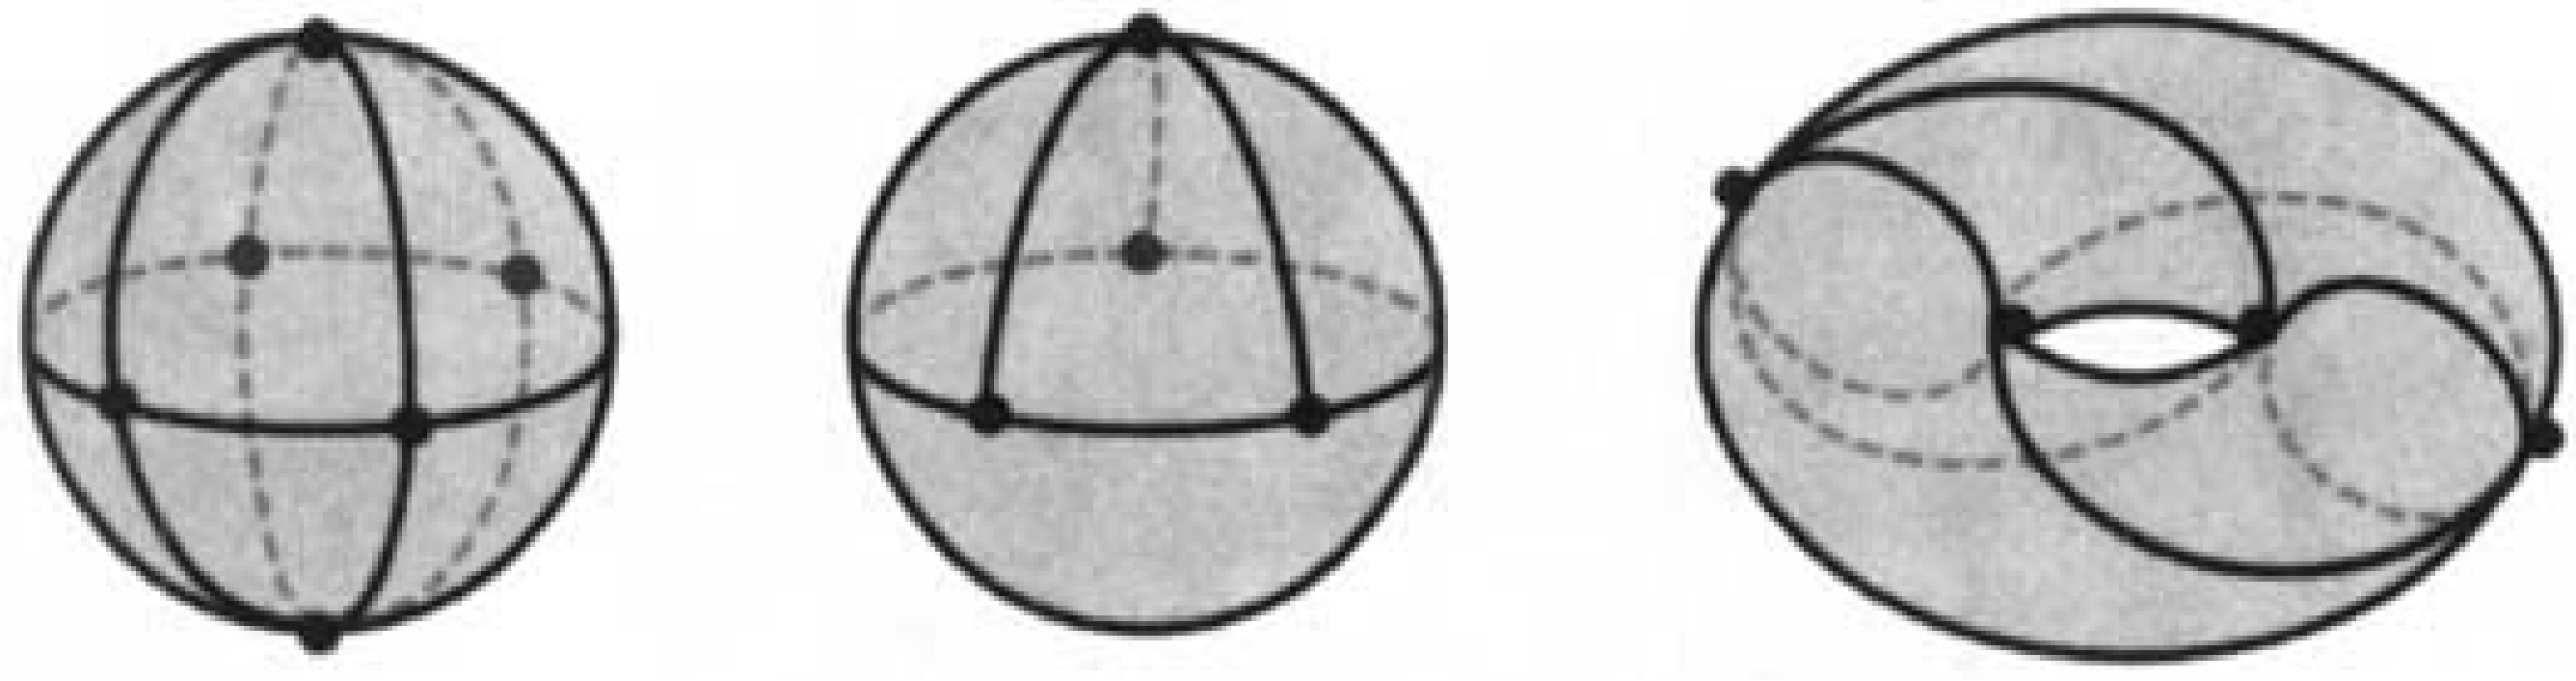
\includegraphics[width=0.6\linewidth]{Blender/ex4-5.png}
        \caption{Triangulations of the sphere and the torus.}
        \label{fig:triangulations}
    \end{figure}
    \begin{itemize}
        \item $\chi=4-6+4=2$
    \end{itemize}
    \item \emph{Exercise 4.6}: Compute the Euler characteristic of the triangulation of the torus in Figure \ref{fig:triangulations}.
    \begin{itemize}
        \item $\chi=4-12+8=0$
    \end{itemize}
    \item The sameness of the Euler characteristics of the two triangulations of the sphere exemplifies the fact the the Euler characteristic depends only on the surface, not the triangulation.
    \item A summary of the proof that any two triangulations have the same Euler characteristic follows.
    %image with this proof?
    \begin{itemize}
        \item Take $T_1$ and $T_2$, two different triangulations of a surface. We will overlay them and add appropriate edges (to make triangles) to make $T_3$. This process will prove that $T_1$ and $T_3$ have the same Euler characteristic. Since $T_2$ could have $T_1$ overlayed, $T_2$ and $T_3$ also have the same Euler characteristic. Therefore, $T_1$ and $T_2$ have the same Euler characteristic (transitive property).
        \item Each edge of $T_2$ intersects $T_1$ a finite number of times, and no vertices are overlaid --- this can be assured by shifting where $T_2$ is overlaid by a slight bit.
        \item Add vertices at the intersections of edges. The addition of one vertex and the subsequent splitting of one edge into two cancel out in the Euler characteristic.
        \item Add the vertices of $T_2$ and a corresponding new edge to each. These edges should be a subset of the edges in $T_2$. Vertices increase by 1 for each vertex and edges increase by 1 for each edge, so the change likewise cancels out.
        \item Add the rest of the edges from $T_2$. Note that for every edge added, a face is split in two, canceling out the change.
        \item Add edges to split all $n$-gon faces into triangles. Each added edge splits a face, so the change, again, cancels out.
        \item Q.E.D.
    \end{itemize}
    \item $\chi(\text{genus}=0)=2$.
    \item $\chi(\text{genus}=1)=0$.
    \item For a genus 2 surface, we could find a triangulation and calculate $\chi$, or we could be clever.
    \item \textbf{Connected sum}: Remove a disk from each of two objects and then glue them together.
    \item With triangulations of two tori, we can imagine that a genus 2 surface can be created via the connected sum of the two tori minus two matching faces.
    \item So, $F\rightarrow F-2$, and because 3 vertices and 3 edges are merged, $V\rightarrow V-3$ and $E\rightarrow E-3$. The vertices and edges cancel out, giving the following property.
    \begin{equation}
        \chi(S)=\chi\left( S_1 \right)+\chi\left( S_2 \right)-2
    \end{equation}
    \item Therefore, $\chi(\text{genus}=2)=-2$.
    \item \emph{Exercise 4.8}: Use connected sums to show that the Euler characteristic of a genus 3 surface is $-4$.
    \begin{itemize}
        \item $S_{\text{genus}=2}+S_{\text{genus}=1}=S_{\text{genus}=3}$.
        \item $\chi\left( S_{\text{genus}=3} \right)=\chi\left( S_{\text{genus}=2} \right)+\chi\left( S_{\text{genus}=1} \right)-2=-2+0-2=-4$.
    \end{itemize}
    \item \emph{Exercise 4.9}: Use induction to show that the Euler characteristic of a surface of genus $g$ is $2-2g$.
    \begin{itemize}
        \item Basis step: $2\overset{\checkmark}{=}2-2(0)$.
        \item Induction hypothesis: $\chi\left( S_{\text{genus}=g} \right)=2-2g$
        \item Induction step:
        \begin{align*}
            \chi\left( S_{\text{genus}=g+1} \right) &\overset{?}{=} 2-2(g+1)\\
            \chi\left( S_{\text{genus}=g} \right)+\chi\left( S_{\text{genus}=1} \right)-2 &\overset{?}{=} 2-2g-2\\
            (2-2g)+0-2 &\overset{?}{=} 0-2g\\
            0-2g &\overset{\checkmark}{=} 0-2g
        \end{align*}
        \item Therefore, the following equation holds true.
        \begin{equation}\label{eqn:chig}
            \chi(g)=2-2g
        \end{equation}
    \end{itemize}
    \item Every surface has a triangulation.
    \item \textbf{Compact} (surface): A surface with a triangulation with a finite number of triangles.
    \item A plane and torus minus a disk are both noncompact surfaces.
    \item Surfaces appear in knot theory in the space around a knot.
    \item \textbf{Complement} (of the knot): The space around the knot $M=\mathbb{R}^3-K$, where $\mathbb{R}^3$ is the three-dimensional space around the knot $K$.
    \item A splittable link can be defined as a link such that there exists a sphere in the link complement between the two link components.
    \item Every knot is contained within a torus. Some knots can be surrounded by a torus in unusual ways or by a genus $2+$ surface.
    \item We are particularly interseted in the surfaces that cannot be simplified.
    \item \textbf{Compressible} (surface): For a link $L$, a surface $F$ where there exists \dq{a disk $D$ in $\mathbb{R}^3-L$ such that $D$ intersects $F$ exactly in its boundary and its boundary does not bound another disk on $F$. Note that $D$ is not allowed to intersect $L$}{86}
    \item \textbf{Compression}: The simplifying operation of cutting $F$ along $D$, gluing $D$ to each open curve, and using an isotropy to "smooth out" the surface.
    \item \emph{Exercise 4.11}: Show that a compression always increases the Euler characteristic. Use this to show that the genus of the resulting surface or surfaces is always less than the genus of the original surface.
    \begin{itemize}
        \item Think of $D$ as a triangle. During the compression, three vertices and three edges separate into two \emph{pairs} of three vertices and three edges. This does not change the Euler characteristic.
        \item However, two faces are also added. This increases the Euler characteristic by 2.
        \item This change of $+2$ changes the genus by $-1$.
    \end{itemize}
    \item \textbf{Incompressible} (surface): A surface that is not compressible.
    \item Any time we have a composite knot, there exists an incompressible \textbf{swallow-follow torus}.
    %swallow-follow torus image
    \item \textbf{Swallow-follow torus}: A torus that encompases (swallows) one factor knot and wraps around the strand of (follows) the other factor knot.
\end{itemize}


\subsection{Surfaces with Boundary}
\begin{itemize}
    \item \textbf{Boundary component}: Discs (that may have been deformed) that have been removed from surfaces.
    \item The Euler characteristic of a surface with boundary is that of that surface without boundary minus the number of boundary components.
    \begin{itemize}
        \item Think of adding each boundary component as removing the face of a triangle.
    \end{itemize}
    \item \textbf{Capping off} (a surface with boundary): \dq{Filling in boundary components by attaching disks}{88}
    \item \emph{Exercise 4.13}: Find the Euler characteristics of each of the surfaces in Figure \ref{fig:boundcomps} without triangulating them.
    \begin{figure}[h!]
        \centering
        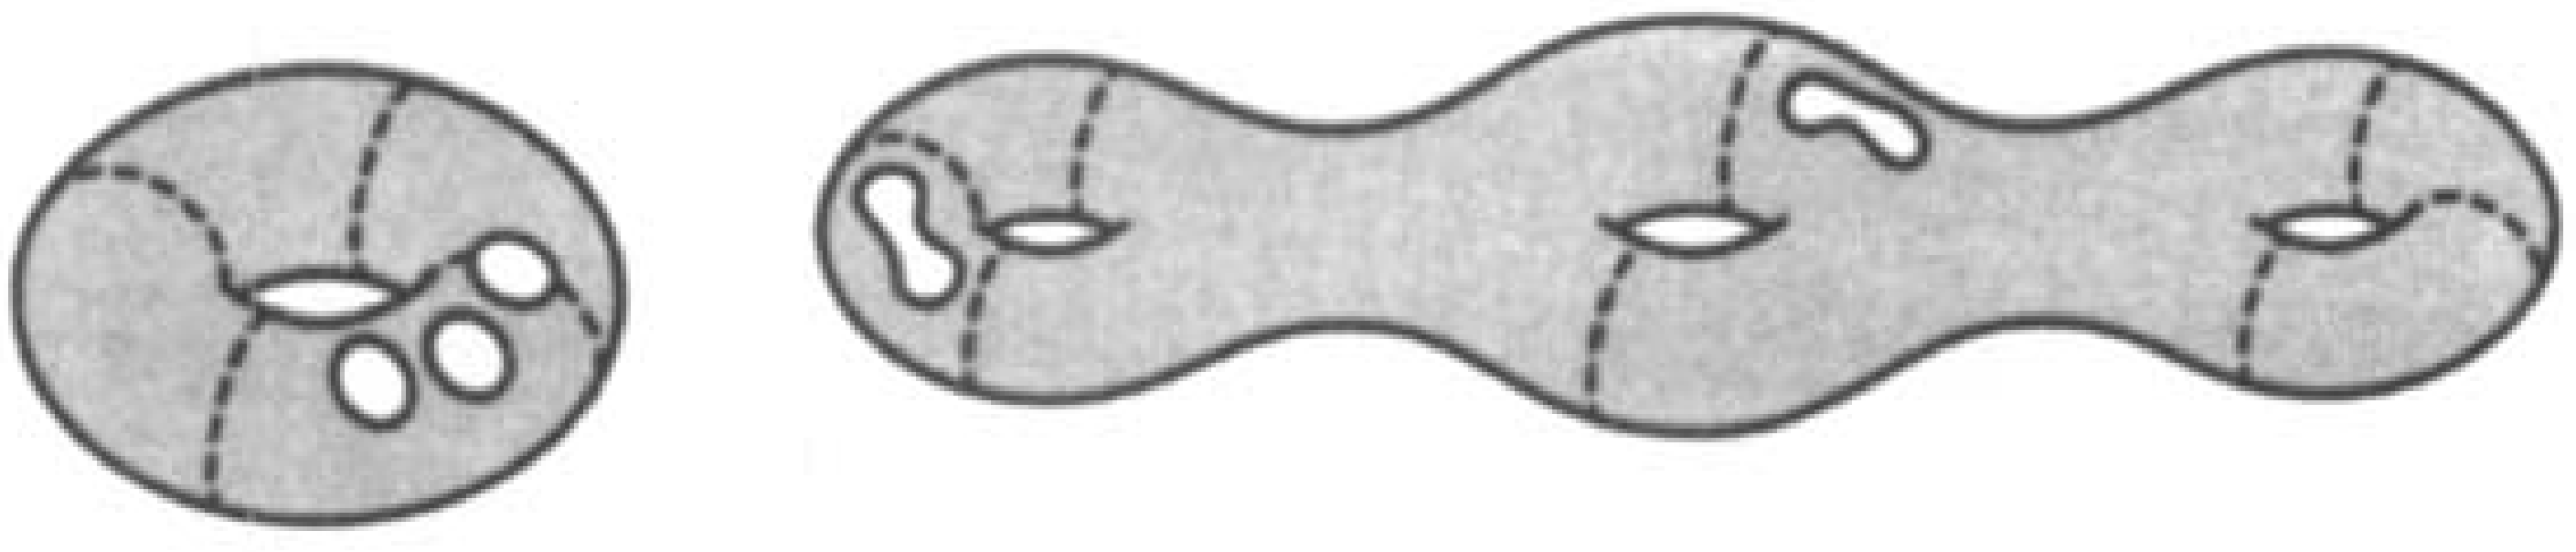
\includegraphics[width=0.6\linewidth]{Blender/ex4-13.png}
        \caption{Surfaces with boundary.}
        \label{fig:boundcomps}
    \end{figure}
    \begin{itemize}
        \item The left surface is a genus 1 surface with three boundary components. Therefore, it has $\chi=0-3=-3$.
        \item The right surface is a genus 3 surface with two boundary components. Therefore, it has $\chi=-4-2=-6$.
    \end{itemize}
    \item The Euler characteristic does not definitively distinguish surfaces with boundary.
    \item There are other ways, such as \textbf{orientability}.
    \item \textbf{Orientable} (surface): A surface sitting in $\mathbb{R}^3$ with \dq{two sides that can be painted different colors, say black and white, so that the black paint never meets the white paint except along the boundary of the surface}{90}
    \begin{itemize}
        \item For example, a disk and a torus are both orientable.
        \item Furthermore, any torus with any number of boundary components is orientable.
    \end{itemize}
    \begin{figure}[h!]
        \centering
        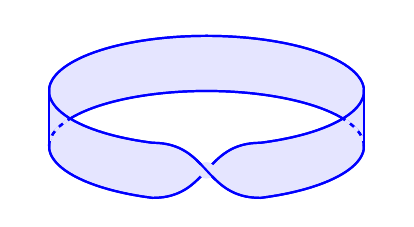
\begin{tikzpicture}
            \fill [blue!10] (0,0)
                arc [start angle=-70,end angle=250,x radius=2cm,y radius=0.7cm]
                to [out=0,in=180,looseness=1.2] (0,-0.7)
                arc [start angle=-70,end angle=250,x radius=2cm,y radius=0.7cm]
                to [out=0,in=180,looseness=1.2] cycle
            ;
            \fill [blue!10] (-2.685,0.694) rectangle (-2,-0.043);
            \fill [blue!10] (0.5,0.694) rectangle (1.315,-0.043);
            \fill [white] (1.05,0.3)
                arc [start angle=30,end angle=150,x radius=2cm,y radius=0.7cm]
                arc [start angle=210,end angle=330,x radius=2cm,y radius=0.7cm]
            ;
            \fill [white] (0,0)
                to [out=180,in=45] (-0.68,-0.35)
                to [out=135,in=0] (-1.4,0)
            ;
            \begin{knot}[
                clip width=8,
                clip radius=3pt,
                consider self intersections,
                background color=blue!10
            ]
                \strand [draw=blue,thick] (0,0)
                    arc [start angle=-70,end angle=250,x radius=2cm,y radius=0.7cm]
                    to [out=0,in=180,looseness=1.2] (0,-0.7)
                    arc [start angle=-70,end angle=250,x radius=2cm,y radius=0.7cm]
                    to [out=0,in=180,looseness=1.2] cycle
                ;
            \end{knot}
            \draw [blue,thick,dash pattern= on 2pt off 2pt,postaction={draw,blue!10,dash pattern= on 2pt off 2pt,dash phase=2pt,line width=1.1pt}] (-2.685,-0.043) arc [start angle=180,end angle=150,x radius=2cm,y radius=0.7cm];
            \draw [blue,thick,dash pattern= on 2pt off 2pt,postaction={draw,blue!10,dash pattern= on 2pt off 2pt,dash phase=2pt,line width=1.1pt}] (1.315,-0.043) arc [start angle=0,end angle=30,x radius=2cm,y radius=0.7cm];
            %applicability to tricolorability?
            \draw [blue,thick] (1.315,0.694) -- (1.315,-0.043);
            \draw [blue,thick] (-2.685,0.694) -- (-2.685,-0.043);
        \end{tikzpicture}
        \caption{A M\"{o}bius band.}
        \label{fig:mobius}
    \end{figure}
    \item \textbf{M\"{o}bius band}: One of the simplest surfaces that is not orientable (see Figure \ref{fig:mobius}).
    \item \dq{A surface is nonorientable if and only if it contains a M\"{o}bius band within it}{91}
    \item A M\"{o}bius band must have an odd number of half-twists in it.
    \item \emph{Exercise 4.15}: Decide which of the two surfaces in Figure \ref{fig:orients} is orientable and which is nonorientable.
    \begin{figure}[H]
        \centering
        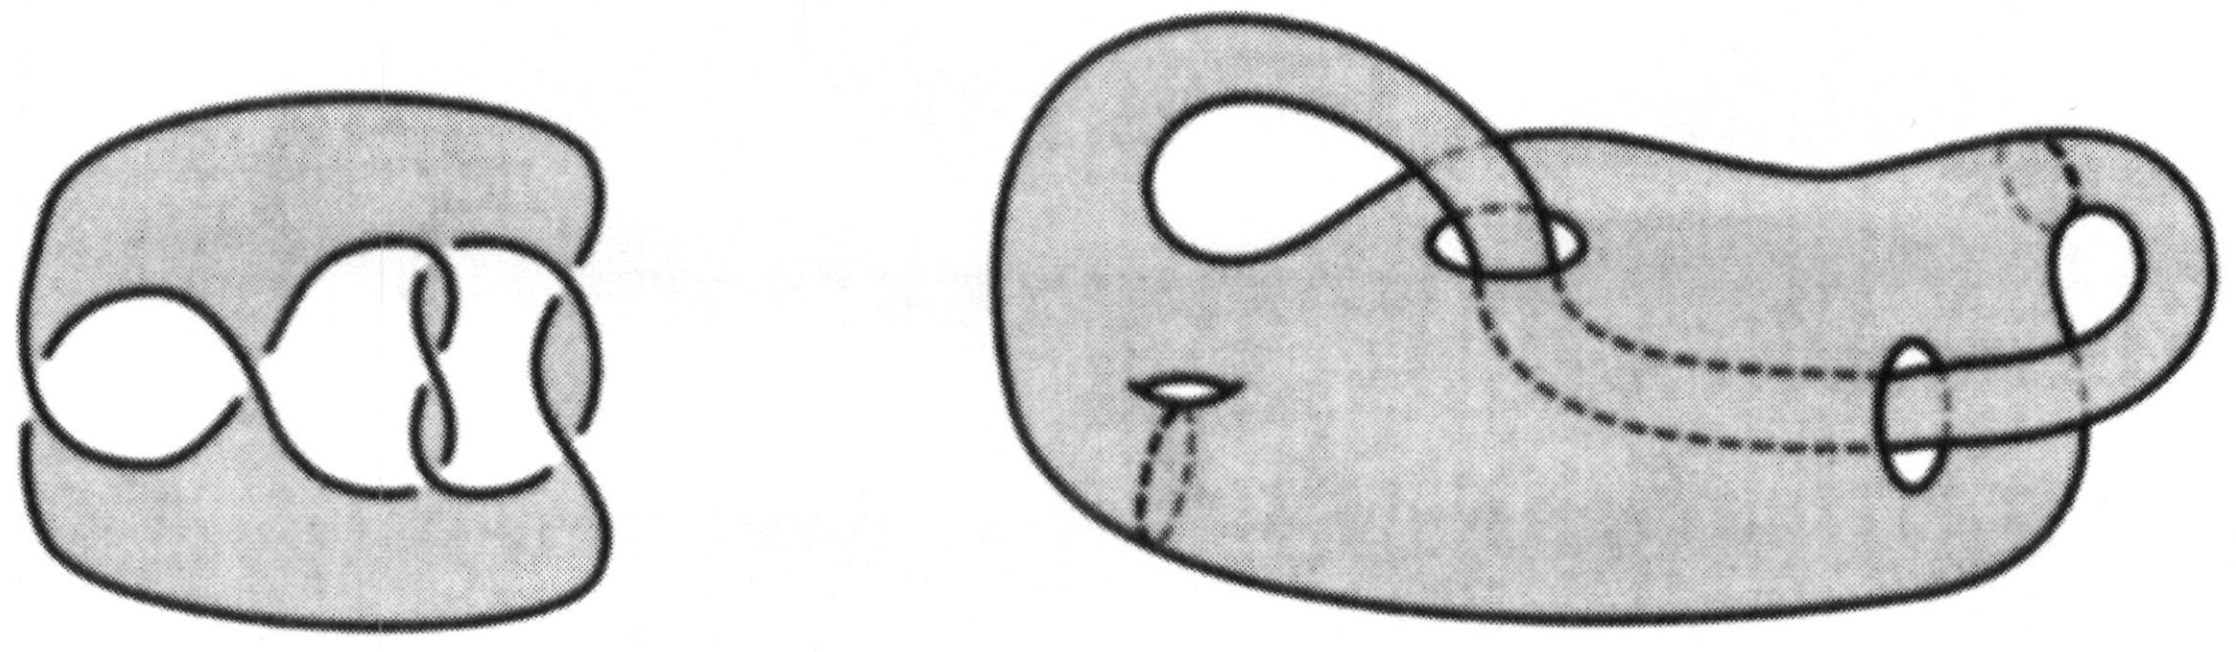
\includegraphics[width=0.6\linewidth]{Blender/ex4-15.png}
        \caption{Possibly orientable surfaces.}
        \label{fig:orients}
    \end{figure}
    \begin{itemize}
        \item The surface on the left is nonorientable while the one on the right is orientable.
    \end{itemize}
    \item Three facts completely determine the homeomorphic type of a surface with boundary.
    \begin{enumerate}
        \item \dq{Is it orientable or nonorientable?
        \item How many boundary components does it have?
        \item What is its Euler characteristic?}{92}
    \end{enumerate}
    \item My techniques:
    \begin{itemize}
        \item Choose a subdivision that has one chord for every twist between boundary components.
        \begin{itemize}
            \item Alternatively, for simpler counting at the expense of bigger numbers, choose two chords at every twist.
        \end{itemize}
        \item Count edges along each boundary component and then count the chords.
    \end{itemize}
    \item \emph{Exercise 4.16}: Use the three criteria to identify the surface with boundary in Figure \ref{fig:boundsurfidenta}.
    \begin{figure}[h!]
        \centering
        \begin{subfigure}[b]{0.3\linewidth}
            \centering
            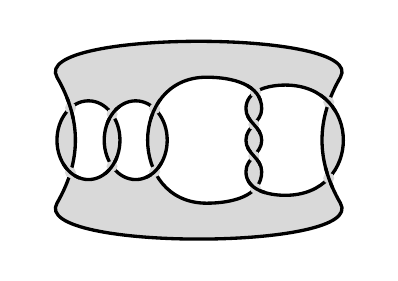
\begin{tikzpicture}
                \colorlet{blx}{black}
                \colorlet{bly}{blx!15}
    
                \fill [bly] (-0.4,0.8)
                    to [out=120,in=60,looseness=0.5] (3.2,0.8)
                    to [out=-120,in=120] (3.2,-0.8)
                    to [out=-60,in=-120,looseness=0.5] (-0.4,-0.8)
                    to [out=60,in=-60] cycle
                ;
                \fill [bly] (0,0) ellipse (4mm and 5mm);
                \fill [bly] (2.5,0.7)
                    to [out=0,in=0,looseness=1.8] (2.5,-0.7)
                    to [out=180,in=-90] (2,-0.4)
                    to [out=90,in=-90] (2.2,0)
                    to [out=90,in=-90] (2,0.4)
                    to [out=90,in=180] cycle
                ;
                \fill [white] (-0.22,0.4)
                    to [out=40,in=120] (0.3,0.33)
                    to [out=-120,in=120] (0.3,-0.33)
                    to [out=-120,in=-45] (-0.22,-0.4)
                    to [out=75,in=-75] cycle
                ;
                \fill [white] (0.3,0.33)
                    to [out=60,in=135] (0.84,0.4)
                    to [out=-110,in=110] (0.84,-0.4)
                    to [out=-135,in=-50] (0.3,-0.33)
                    to [out=60,in=-60] cycle
                ;
                \fill [white] (0.84,0.4)
                    to [out=60,in=135] (2.12,0.6)
                    to [out=-150,in=150] (2.1,0.2)
                    to [out=-135,in=135] (2.1,-0.2)
                    to [out=-150,in=150] (2.12,-0.6)
                    to [out=-135,in=-60] (0.84,-0.4)
                    to [out=50,in=-50] cycle
                ;
                \fill [white] (3.05,0.48)
                    to [out=135,in=30] (2.12,0.6)
                    to [out=-50,in=50] (2.1,0.2)
                    to [out=-50,in=50] (2.1,-0.2)
                    to [out=-50,in=50] (2.12,-0.6)
                    to [out=-30,in=-135] (3.05,-0.48)
                    to [out=110,in=-110] cycle
                ;
        
                \begin{knot}[
                    clip width=5,
                    clip radius=2pt,
                    ignore endpoint intersections=false,
                    background color=bly,
                    every strand/.append style={blx,very thick}
                ]
                    \strand (0,0) ellipse (4mm and 5mm);
                    \strand (0.6,0) ellipse (4mm and 5mm);
                    \strand (1.5,0.8)
                        to [out=180,in=180,looseness=1.6] (1.5,-0.8)
                        to [out=0,in=-90] (2.2,-0.4)
                        to [out=90,in=-90] (2,0)
                        to [out=90,in=-90] (2.2,0.4)
                        to [out=90,in=0,] cycle
                    ;
                    \strand (2.5,0.7)
                        to [out=0,in=0,looseness=1.8] (2.5,-0.7)
                        to [out=180,in=-90] (2,-0.4)
                        to [out=90,in=-90] (2.2,0)
                        to [out=90,in=-90] (2,0.4)
                        to [out=90,in=180] cycle
                    ;
                    \strand (-0.4,0.8)
                        to [out=120,in=60,looseness=0.5] (3.2,0.8)
                        to [out=-120,in=120] (3.2,-0.8)
                        to [out=-60,in=-120,looseness=0.5] (-0.4,-0.8)
                        to [out=60,in=-60] cycle
                    ;
                    \flipcrossings{1,3,5,7,9,12}
                \end{knot}
            \end{tikzpicture}
            \caption{A surface.}
            \label{fig:boundsurfidenta}
        \end{subfigure}
        \begin{subfigure}[b]{0.3\linewidth}
            \centering
            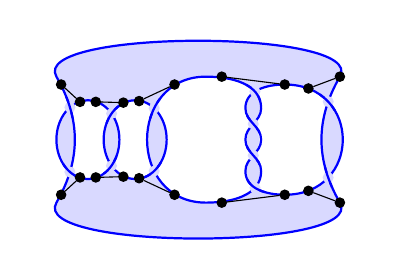
\begin{tikzpicture}
                \colorlet{blx}{blue}
                \colorlet{bly}{blx!15}
                
                \fill [bly] (-0.4,0.8)
                    to [out=120,in=60,looseness=0.5] (3.2,0.8)
                    to [out=-120,in=120] (3.2,-0.8)
                    to [out=-60,in=-120,looseness=0.5] (-0.4,-0.8)
                    to [out=60,in=-60] cycle
                ;
                \fill [bly] (0,0) ellipse (4mm and 5mm);
                \fill [bly] (2.5,0.7)
                    to [out=0,in=0,looseness=1.8] (2.5,-0.7)
                    to [out=180,in=-90] (2,-0.4)
                    to [out=90,in=-90] (2.2,0)
                    to [out=90,in=-90] (2,0.4)
                    to [out=90,in=180] cycle
                ;
                \fill [white] (-0.22,0.4)
                    to [out=40,in=120] (0.3,0.33)
                    to [out=-120,in=120] (0.3,-0.33)
                    to [out=-120,in=-45] (-0.22,-0.4)
                    to [out=75,in=-75] cycle
                ;
                \fill [white] (0.3,0.33)
                    to [out=60,in=135] (0.84,0.4)
                    to [out=-110,in=110] (0.84,-0.4)
                    to [out=-135,in=-50] (0.3,-0.33)
                    to [out=60,in=-60] cycle
                ;
                \fill [white] (0.84,0.4)
                    to [out=60,in=135] (2.12,0.6)
                    to [out=-150,in=150] (2.1,0.2)
                    to [out=-135,in=135] (2.1,-0.2)
                    to [out=-150,in=150] (2.12,-0.6)
                    to [out=-135,in=-60] (0.84,-0.4)
                    to [out=50,in=-50] cycle
                ;
                \fill [white] (3.05,0.48)
                    to [out=135,in=30] (2.12,0.6)
                    to [out=-50,in=50] (2.1,0.2)
                    to [out=-50,in=50] (2.1,-0.2)
                    to [out=-50,in=50] (2.12,-0.6)
                    to [out=-30,in=-135] (3.05,-0.48)
                    to [out=110,in=-110] cycle
                ;
        
                \begin{knot}[
                    clip width=5,
                    clip radius=2pt,
                    ignore endpoint intersections=false,
                    background color=bly,
                    every strand/.append style={blx,thick}
                ]
                    \strand (0,0) ellipse (4mm and 5mm);
                    \strand (0.6,0) ellipse (4mm and 5mm);
                    \strand (1.5,0.8)
                        to [out=180,in=180,looseness=1.6] (1.5,-0.8)
                        to [out=0,in=-90] (2.2,-0.4)
                        to [out=90,in=-90] (2,0)
                        to [out=90,in=-90] (2.2,0.4)
                        to [out=90,in=0,] cycle
                    ;
                    \strand (2.5,0.7)
                        to [out=0,in=0,looseness=1.8] (2.5,-0.7)
                        to [out=180,in=-90] (2,-0.4)
                        to [out=90,in=-90] (2.2,0)
                        to [out=90,in=-90] (2,0.4)
                        to [out=90,in=180] cycle
                    ;
                    \strand (-0.4,0.8)
                        to [out=120,in=60,looseness=0.5] (3.2,0.8)
                        to [out=-120,in=120] (3.2,-0.8)
                        to [out=-60,in=-120,looseness=0.5] (-0.4,-0.8)
                        to [out=60,in=-60] cycle
                    ;
                    \flipcrossings{1,3,5,7,9,12}
                \end{knot}
    
                \begin{scope}[
                    every node/.style={circle,draw,fill,inner sep=1.2pt}
                ]
                    \node (a) at (-0.34,0.7) {};
                    \node at (-0.1,0.48) {}
                        edge (a)
                    ;
                    \node (b) at (0.45,0.47) {};
                    \node at (0.1,0.48) {}
                        edge (b)
                    ;
                    \node (c) at (0.65,0.49) {};
                    \node at (1.1,0.7) {}
                        edge (c)
                    ;
                    \node (d) at (2.5,0.7) {};
                    \node at (1.7,0.8) {}
                        edge (d)
                    ;
                    \node (e) at (2.8,0.65) {};
                    \node at (3.2,0.8) {}
                        edge (e)
                    ;
    
                    \node (f) at (-0.34,-0.7) {};
                    \node at (-0.1,-0.48) {}
                        edge (f)
                    ;
                    \node (g) at (0.45,-0.47) {};
                    \node at (0.1,-0.48) {}
                        edge (g)
                    ;
                    \node (h) at (0.65,-0.49) {};
                    \node at (1.1,-0.7) {}
                        edge (h)
                    ;
                    \node (i) at (2.5,-0.7) {};
                    \node at (1.7,-0.8) {}
                        edge (i)
                    ;
                    \node (j) at (2.8,-0.65) {};
                    \node at (3.2,-0.8) {}
                        edge (j)
                    ;
                \end{scope}
            \end{tikzpicture}
            \caption{A subdivision.}
            \label{fig:boundsurfidentb}
        \end{subfigure}
        \caption{Identifying a surface with boundary.}
        \label{fig:boundsurfident}
    \end{figure}
    \begin{itemize}
        \item Begin by choosing the subdivision in Figure \ref{fig:boundsurfidentb} according to the first technique above.
        \item Count $V=20$, $E=30$, and $F=7$. Count $BC=5$ where $BC$ is the number of boundary components.
        \item Thus, $\chi=-3$. Adding $+1$ to $\chi$ for every boundary component, find $\chi$ for the original surface without boundary to be $2$.
        \item Therefore, the surface without boundary corresponding to Figure \ref{fig:boundsurfidenta} is the sphere.
    \end{itemize}
    \item Define the genus of a surface with boundary to be that of the surface without boundary obtained by capping off each of its boundary components.
    \item Coming back to knot theory, one way to define knots is as the boundary of surfaces, i.e., the unknot could be defined as the boundary of a disk.
    \item \textbf{Annulus}: A sphere with two boundary components that lies outside one of the factor knots in a composite knot.
    \begin{itemize}
        \item Note that this definition necessitates that the knot be thickened from a one-manifold.
        \item Otherwise, an annulus would be a sphere with two punctures.
    \end{itemize}
    \item Therefore, another definition of composite knot is \dq{a knot such that there is a sphere in space punctured twice by the knot such that the knot is nontrivial both inside and outside the sphere}{93}
    \item \textbf{Conway sphere}: A sphere with four punctures enclosing a tangle.
    \begin{itemize}
        \item This is the $\mathbb{R}^3$ analogy to the cyan circles in the projection plane in Figure \ref{fig:tangles}.
        \item If the knot is thickened, the Conway sphere becomes a sphere with four boundary components.
    \end{itemize}
    \begin{figure}[h!]
        \centering
        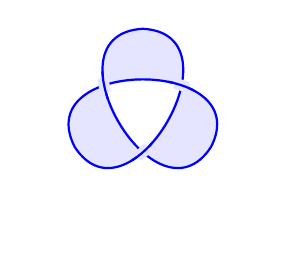
\begin{tikzpicture}
            \colorlet{blx}{blue}
            \colorlet{bly}{blx!10}
    
            \fill [bly] (90:1)
                \foreach \x in {1,2,3} {
                    to [bend left=117,looseness=1.9] ({90+120*\x}:1)
                }
            ;
            \fill [white] (30:0.57)
                \foreach \x in {1,2,3} {
                    to [bend left=10] ({30-120*\x}:0.57)
                }
            ;
    
            \begin{knot}[
                clip width=5,
                clip radius=3pt,
                background color=bly,
                every strand/.append style={blx,thick},
                consider self intersections
            ]
                \strand (90:1)
                    \foreach \x in {1,2,3} {
                        to [bend left=117,looseness=1.9] ({90+120*\x}:1)
                    }
                ;
                \flipcrossings{1,3}
            \end{knot}
        \end{tikzpicture}
        \vspace{-0.7cm}
        \caption{The trefoil as a M\"{o}bius band.}
        \label{fig:trefoilmobius}
    \end{figure}
    \item Continuing with the idea that a disk defines the unknot, the trefoil knot (for instance) can be defined as the boundary of a M\"{o}bius band of three half-twists, as in Figure \ref{fig:trefoilmobius}.
    \item Clearly, of particular interest are orientable surfaces with one boundary component such that said boundary component is a knot.
\end{itemize}


\subsection{Genus and Seifert Surfaces}\label{sss:GenusSeifert}
\begin{itemize}
    \item There is one type of surface that appears in the complement of any knot.
    \begin{itemize}
        \item In 1934, Herbert Seifert developed \dq{an algorithm so that, given any knot, one can create an orientable surface with one boundary component such that the boundary circle is that knot}{95}
    \end{itemize}
    \item Seifert's algorithm is summarized as follows.
    \begin{itemize}
        \item Take a knot and assign an orientation.
        \item Eliminate each crossing by connecting the strand flowing in with the adjacent strand flowing out.
        \item This produces a collection of \textbf{Seifert circles}.
        \item Each circle bounds a disk in a plane. To avoid intersections, raise and lower the disks to different $z$-heights.
        \item Finally, connect the disks to one another at the crossings of the knot by twisted bands.
    \end{itemize}
    \item \textbf{Seifert circle}: A loop that can be deformed into a circle via a planar isotropy.
    \item \emph{Exercise 4.18}: Show that the surface that we get doesn't depend on the direction we choose for the orientation on the knot.
    \begin{figure}[H]
        \centering
        \begin{subfigure}[b]{0.6\linewidth}
            \centering
            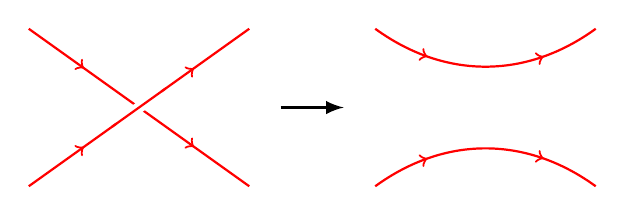
\begin{tikzpicture}
                \draw[very thick,-latex] (-0.4,0) -- (0.4,0);
                \begin{knot}[
                    xshift=-2.2cm,
                    clip width=5,
                    every strand/.append style={
                        red,thick,
                        decoration={markings,
                            mark=at position 0.25 with \arrow{>},
                            mark=at position 0.75 with \arrow{>}
                        },
                        postaction={decorate}
                    }
                ]
                    \strand (-1.4,-1) to (1.4,1);
                    \strand (-1.4,1) to (1.4,-1);
                \end{knot}
                \begin{knot}[
                    xshift=2.2cm,
                    clip width=5,
                    clip radius=3pt,
                    every strand/.append style={
                        red,thick,
                        decoration={markings,
                            mark=at position 0.25 with \arrow{>},
                            mark=at position 0.75 with \arrow{>}
                        },
                        postaction={decorate}
                    }
                ]
                    \strand (-1.4,-1) to[out=36,in=144] (1.4,-1);
                    \strand (-1.4,1) to[out=-36,in=-144] (1.4,1);
                \end{knot}
            \end{tikzpicture}
            \caption{Orientation 1.}
            \label{fig:seifertcrossinga}
        \end{subfigure}\\
        \vspace{1em}
        \begin{subfigure}[b]{0.6\linewidth}
            \centering
            \begin{tikzpicture}
                \draw[very thick,-latex] (-0.4,0) -- (0.4,0);
                \begin{knot}[
                    xshift=-2.2cm,
                    clip width=5,
                    every strand/.append style={
                        red,thick,
                        decoration={markings,
                            mark=at position 0.25 with \arrow{<},
                            mark=at position 0.75 with \arrow{<}
                        },
                        postaction={decorate}
                    }
                ]
                    \strand (-1.4,-1) to (1.4,1);
                    \strand (-1.4,1) to (1.4,-1);
                \end{knot}
                \begin{knot}[
                    xshift=2.2cm,
                    clip width=5,
                    clip radius=3pt,
                    every strand/.append style={
                        red,thick,
                        decoration={markings,
                            mark=at position 0.25 with \arrow{<},
                            mark=at position 0.75 with \arrow{<}
                        },
                        postaction={decorate}
                    }
                ]
                    \strand (-1.4,-1) to[out=36,in=144] (1.4,-1);
                    \strand (-1.4,1) to[out=-36,in=-144] (1.4,1);
                \end{knot}
            \end{tikzpicture}
            \caption{Orientation 2.}
            \label{fig:seifertcrossingb}
        \end{subfigure}
        \caption{The relationship between orientation and crossing changes in Seifert's algorithm.}
        \label{fig:seifertcrossing}
    \end{figure}
    \begin{itemize}
        \item At each crossing, two strands flow in and two flow out, regardless of the orientation, as in the left part of both subfigures in Figure \ref{fig:seifertcrossing}. In effect, any crossing can be reworked to resemble the aforementioned parts of subfigures.
        \item One of the strands adjacent to a strand flowing in always flows out and vice versa.
        \item Because of this, reversing the orientation does not change the above fact (compare the left part of Figure \ref{fig:seifertcrossinga} with that of Figure \ref{fig:seifertcrossingb}).
        \item Thus, whatever adjacent strands were paired up before will be paired up again (see the right side of Figures \ref{fig:seifertcrossinga} and \ref{fig:seifertcrossingb}).
        \item Since the Seifert circles determine the final surface, the above proof that said circles will be unchanged verifies that the surfaces will remain unchanged.
    \end{itemize}
    \item The surface is orientable because of the following thought experiment.
    \begin{itemize}
        \item For any circle with a clockwise orientation, paint the upper face white and the lower face black.
        \item For any circle with a counterclockwise orientation, paint the upper face black and the lower face white.
        \item Any two circles above/below one another will have the same orientation, and, thus, the half-twist connects like colored faces.
        \item Any two circles adjacent to each other will have opposite orientations, and, thus, the half-twist connects like colored faces.
        \item Therefore, the surface is orientable.
    \end{itemize}
    \item \emph{Exercise 4.19}: Note that if we add an edge and two vertices to the surface across each crossing, cutting each band in half, we cut the surface up into valid faces. Use this fact to show that if $c$ is the number of crossings and $s$ is the number of Seifert circles, then $\chi=s-c$ and the genus of the surface is $g=\frac{c-s+1}{2}$.
    \begin{itemize}
        \item Every 2-vertices-1-edge addition described above has a predictable effect on $V$ and $E$.
        \begin{itemize}
            \item Each vertex adds one new vertex (obviously), so two vertices are added for each 2-vertices-1-edge addition.
            \item Each vertex splits an existing edge into two edges. Accounting for the addition of the connecting edge, three edges are added for each 2-vertices-1-edge addition.
            \item Since two vertices and three edges are added each time, the quantity $V-E$ changes by $-1$ with each 2-vertices-1-edge addition.
            \item Because, by the problem statement, a 2-vertices-1-edge addition occurs at each crossing, there are $c$ such additions.
            \item Thus, $V-E=-c$ for the entire process.
        \end{itemize}
        \item The final subdivision, on the other hand, reveals something about $F$.
        \begin{itemize}
            \item Each face is separated from the others at the crossings.
            \item Thus, since each face is composed of a Seifert circle plus a bit of twisting connection, the number of faces corresponds to the the original number of Seifert circles $s$, or $F=s$.
        \end{itemize}
        \item Therefore, the sum of the derived values can be substituted into the sum $V-E+F$ to yield $-c+s$ or $s-c$.
        \item Since Equation \ref{eqn:eulerchar} gives us $\chi=V-E+F$, the following equation holds by the transitive property.
        \begin{equation}\label{eqn:chisc}
            \chi=s-c
        \end{equation}
        \item According to Equation \ref{eqn:chig}, $\chi=2-2g$, so $g=\frac{2-\chi}{2}$.
        \begin{itemize}
            \item However, the genus of a surface with boundary is that of the surface without boundary acquired via capping off said surface with boundary.
            \item Since the surface at hand is known to have specifically one boundary component, the $\chi$ that should presently be considered is the $\chi$ of the previous part plus one, or $\chi_1=s-c+1$.
        \end{itemize}
        \item Substitute: $g=\frac{2-(s-c+1)}{2}$.
        \item Simplify.
        \begin{align*}
            g &=\frac{2-(s-c+1)}{2}\\
            &=\frac{2-s+c-1}{2}\\
            g &=\frac{c-s+1}{2}\stepcounter{equation}\tag{\theequation}\label{eqn:gensei}
        \end{align*}
    \end{itemize}
    \item \emph{Exercise 4.21}: Show that Seifert's algorithm always generates at least two Seifert circles.
    \begin{figure}[h!]
        \centering
        \begin{subfigure}[b]{0.27\linewidth}
            \centering
            \begin{tikzpicture}
                \node (a) at (-1,0) [circle,draw=red,thick,fill=orange!50] {$L_1$};
                \node (b) at (1,0)  [circle,draw=red,thick,fill=orange!50] {$L_2$};
                \begin{knot}[
                    clip width=5,
                    every strand/.append style={red,thick}
                ]
                    \strand ([xshift=-0.5pt]a.45) to[out=0,in=180] ([xshift=0.5pt]b.-135);
                    \strand ([xshift=-0.5pt]a.-45) to[out=0,in=180] ([xshift=0.5pt]b.135);
                \end{knot}
            \end{tikzpicture}
            \caption{Two connected loops.}
            \label{fig:Scirccrossa}
        \end{subfigure}
        \begin{subfigure}[b]{0.27\linewidth}
            \centering
            \begin{tikzpicture}
                \node (a) at (-1,0) [circle,draw=red,thick,fill=orange!50] {$L_1$};
                \node (b) at (1,0)  [circle,draw=red,thick,fill=orange!50] {$L_2$};
                \begin{knot}[
                    clip width=5,
                    every strand/.append style={
                        red,thick,postaction={decorate}
                    }
                ]
                    \strand [
                        decoration={markings,
                            mark=at position 0.25 with \arrow{<},
                            mark=at position 0.75 with \arrow{<}
                        }
                    ] ([xshift=-0.5pt]a.45) to[out=0,in=180] ([xshift=0.5pt]b.-135);
                    \strand [
                        decoration={markings,
                            mark=at position 0.25 with \arrow{>},
                            mark=at position 0.75 with \arrow{>}
                        },
                    ] ([xshift=-0.5pt]a.-45) to[out=0,in=180] ([xshift=0.5pt]b.135);
                \end{knot}
            \end{tikzpicture}
            \caption{An orientation.}
            \label{fig:Scirccrossb}
        \end{subfigure}
        \begin{subfigure}[b]{0.27\linewidth}
            \centering
            \begin{tikzpicture}
                \node (a) at (-1,0) [circle,draw=red,thick,fill=orange!50] {$L_1$};
                \node (b) at (1,0)  [circle,draw=red,thick,fill=orange!50] {$L_2$};
                \begin{knot}[
                    clip width=5,
                    every strand/.append style={
                        red,thick,postaction={decorate}
                    }
                ]
                    \strand [
                        decoration={markings,
                            mark=at position 0.25 with \arrow{<},
                            mark=at position 0.75 with \arrow{<}
                        }
                    ] ([xshift=-0.5pt]a.45) to[out=0,in=0,looseness=3] ([xshift=-0.5pt]a.-45);
                    \strand [
                        decoration={markings,
                            mark=at position 0.25 with \arrow{>},
                            mark=at position 0.75 with \arrow{>}
                        },
                    ] ([xshift=0.5pt]b.-135) to[out=180,in=180,looseness=3] ([xshift=0.5pt]b.135);
                \end{knot}
            \end{tikzpicture}
            \caption{Two Seifert circles.}
            \label{fig:Scirccrossc}
        \end{subfigure}
        \caption{Generating Seifert circles from a crossing.}
        \label{fig:Scirccross}
    \end{figure}
    \begin{itemize}
        \item In any knot with $c(K)>0$, there exists a region with a crossing between two (possibly knotted) loops $L_1$ and $L_2$, as in Figure \ref{fig:Scirccrossa}.
        \item When assigning an orientation to this crossing, the directions on the subarcs \emph{must} be reversed.
        \begin{itemize}
            \item If they both flowed from left to right (for example), that would imply that there is some point in $L_1$ from which the orientation "flows outward" in both directions and some point in $L_2$ to which the orientation "flows inward" from both directions.
            \item This is contrary to the definition of an orientation, and, therefore, cannot be the case.
        \end{itemize}
        \item Thus, the orientation in Figure \ref{fig:Scirccrossb} is valid.
        \item Given this orientation, the subarcs must separate into two Seifert circles, as in Figure \ref{fig:Scirccrossc}, according to Seifert's algorithm.
        \item This separation would hold for the opposite orientation, as demonstrated by Figure \ref{fig:seifertcrossing}.
    \end{itemize}
    \item It is possible to create multiple different-looking surfaces for the same knot by having a different starting projection.
    \item \textbf{Seifert surface} (for $K$): Given a knot $K$, \dq{an orientable surface with one boundary component such that the boundary component of the surface is the knot $K$}{99}
    \item \textbf{Genus} (of a knot): \dq{The least genus of any Seifert surface for that knot}{99}
    \item The unknot has genus 0 (and is the only knot with genus 0).
    \item Seifert's algorithm yields a Seifert surface of genus 1 for the figure-eight knot, and since the figure-eight knot is nontrivial, no Seifert surface of lower genus can exist for it. Therefore, the genus of the figure-eight knot is 1.
    \item \emph{Exercise 4.22}: The twist knots are the knots obtained by linking together the two ends of a twisted loop. They include the trefoil and figure-eight knots. Show that all of the twist knots have genus 1.
    \begin{figure}[h!]
        \centering
        \begin{tikzpicture}
            \begin{knot}[
                clip width=5,
                clip radius=3pt,
                consider self intersections,
                ignore endpoint intersections=false
            ]
                \strand [red,thick] (-0.3,1)
                    to [out=-5,in=90] (0.2,0.5)
                    to [out=-90,in=90] (-0.2,-0.5)
                    to [out=-90,in=-90,looseness=3] (0.2,-0.5)
                    to [out=90,in=-90] (-0.2,0.5)
                    to [out=90,in=-175] (0.3,1)
                    to [out=5,in=0,out looseness=1.7,in looseness=2.2] (0,-0.7)
                    to [out=180,in=175,out looseness=2.2,in looseness=1.7] cycle
                ;
                \flipcrossings{3,5}
            \end{knot}
            \node [fill=white,inner sep=3mm] at (0,0.1) {\Huge$\vdots$};
        \end{tikzpicture}
        \caption{The general twist knot.}
        \label{fig:twistknots}
    \end{figure}
    \begin{itemize}
        \item This demonstration will follow the format of an induction proof. By Equation \ref{eqn:gensei}, if $g=1$ for a knot, then $s=c-1$. This argument will prove by induction that $s=c-1$.
        \item Every twist knot can be projected in the mold of Figure \ref{fig:twistknots}, where the dots are replaced by some number of twists.
        \item For the trefoil knot, this number of twists is 0 and $s\overset{\checkmark}{=}c-1$.
        \item Each new twist obviously adds one crossing.
        \item This new crossing, when the knot is assigned an orientation, will perfectly match one of the two left images in Figure \ref{fig:seifertcrossing}.
        \begin{itemize}
            \item This is because the orientation weaves its way down all of one of the two "vertical-ish" strands and then changes direction at the bottom loop to weave its way back up.
        \end{itemize}
        \item Like in Figure \ref{fig:seifertcrossing}, Seifert's algorithm will yield one of the two products --- separate loops.
        \item Thus, because every new crossing adds a new place to separate loops, both $s$ and $c$ increase by $+1$ in each subsequent twist knot.
        \item Therefore, since $s+1=c+1-1$, $s$ always equals $c-1$.
    \end{itemize}
    \item \emph{Exercise 4.23}: Show that a minimal genus Seifert surface for a knot $K$ must be incompressible (consider Euler characteristic).
    \begin{itemize}
        \item Proof by contradiction: Take a compressible Seifert surface $F$ for a knot $K$ of minimal genus $g_0$.
        \item Compress it, adding $+2$ to the Euler characteristic $\chi_0$ to get $\chi_1=\chi_0+2$.
        \item By Equation \ref{eqn:chig}, the following holds.
        \begin{align*}
            \chi_0 &=2-2g_0\\
            \chi_1 &=2-2g_1\\
            \chi_0+2 &=2-2g_1\\
            2-2g_0 &=-2g_1\\
            g_1 &=g_0-1\\
            g_1 &<g_0
        \end{align*}
        \item But since no genus $g$ for $K$ can be lower than $g_0$ by $g_0$'s definition as minimal, we have arrived at a contradiction.
        \item Therefore, the minimal genus Seifert surface must be incompressible.
    \end{itemize}
    \item \dq{Applying Seifert's algorithm to an alternating projection of an alternating knot or link does yield a Seifert surface of minimal genus}{100}
    \item The following equation holds.
    \begin{equation}\label{eqn:genuscomp}
        g(J\#K)=g(J)+g(K)
    \end{equation}
    \begin{itemize}
        \item Clearly, $g(J\#K)\leq g(J)+g(K)$ because taking the composition of the two Seifert surfaces does not add any vertices, edges, or faces.
        \item \emph{Isotope surfaces, clean up intersections, perform surgeries to lower the number of intersection curves}$^[$\footnote{Return to at a later date. Perhaps surgeries always increase Euler characteristic, lowering genus, until $g(J)$ and $g(K)$ are both at their minimum. Then their sum must be less than or equal to their composition?}$^]$.
        \item Arrive at $g(J)+g(K)\leq g(J\#K)$.
        \item Therefore, $g(J\#K)=g(J)+g(K)$.
    \end{itemize}
    \item Referencing Section \ref{sss:Composition}, the trivial knot cannot be the composition of two nontrivial knots because $g(K)\geq 1$ where $K$ is nontrivial, so by Equation \ref{eqn:genuscomp}, $g(J\#K)\geq 2>0\Rightarrow g(J\#K)$ is nontrivial.
    \item \emph{Exercise 4.27}: Show that the genus 1 knots are prime.
    \begin{itemize}
        \item For a knot to be nontrivial, its genus must be greater than or equal to 1.
        \item For a knot to be composite, its genus must be greater than or equal to 2.
        \item Therefore, all knots with genus 1 have a high enough genus to be nontrivial (prime or composite) but not a low enough genus to not be composite (they are only prime).
    \end{itemize}
    \item \emph{Exercise 4.28}: Prove that if we take the composition of $n$ copies of the same nontrivial knot, calling the result $J_n$, then as $n\rightarrow\infty$, $c(J_n)\rightarrow\infty$. Hint: Use the fact that there are only a finite number of knots with a given crossing number, but first use the Dowker notation to prove this fact.
    \begin{itemize}
        \item For $c(K)=n$, the Dowker notation will consist of $n$ even numbers ranging from $2$ to $2n$. Therefore, there are $n$ possibilities for the first number, $n-1$ for the second number, and so on and so forth. This compresses down to $n!$ possible knots of $c(K)=n$.
        \begin{itemize}
            \item Note that a large number of these knots will not be of this crossing number. This is an upper bound in the most literal sense.
        \end{itemize}
        \item One way to prove this would be to use Equation \ref{eqn:genuscomp} to prove that the genus must increase with successive compositions. Since the genus is directly proportional to the quantity $c-s$ (by Equation \ref{eqn:gensei}), $c-s$ must increase with successive compositions. Since $s$ cannot decrease with successive compositions (and certainly cannot decrease infinitely), $c$ must increase with successive compositions.
        \item I believe that the desired way to prove this is as follows. Composite knots are distinct from their factor knots. Generating a new composite knot creates a new knot. Since there are a finite number of knots of $c(K)=n$, eventually, all low-crossing possibilities (which will not all be reached, but regardless) must be used up. This forces $c(K)$ higher and higher as new knots are created.
    \end{itemize}
    \item \emph{Exercise 4.29}: Prove that if $J_n$ is the composition of $n$ copies of the same nontrivial knot, then $c(J_n)\geq n$. Hint: Use the Euler characteristic of a Seifert surface along with Equations \ref{eqn:chisc} and \ref{eqn:gensei} and \emph{Exercise 4.21}. Subsequently, prove that $c(J_n)\geq 2n+1$.
    \begin{itemize}
        \item See the first solution to Exercise 4.28.
    \end{itemize}
    \item Seifert's algorithm's applicability to finding genus has been extended from alternating links to \textbf{alternative links}, which also include all \textbf{torus links} (see Section \ref{sss:TorusKnots}).
    \item There are some knots from which the minimal genus Seifert surface cannot be obtained using Seifert's algorithm on any projection of said knot.
    \item \textbf{Canonical genus} (of a knot): \dq{The minimal genus of any Seifert surface obtained by applying Seifert's algorithm to a projection of the knot}{106} \emph{Also known as} $g_c(K)$.
    \item Genus was used to tell apart the Kinoshita-Terasaka mutants (see Section \ref{sss:Conway}).
\end{itemize}
\newpage



\section{Types of Knots}
\subsection{Torus Knots}\label{sss:TorusKnots}
\begin{itemize}
    \item \textbf{Torus knot}: A knot that lies on an unknotted torus such that the subarcs do not cross each other on the torus's surface.
    \begin{figure}[h!]
        \centering
        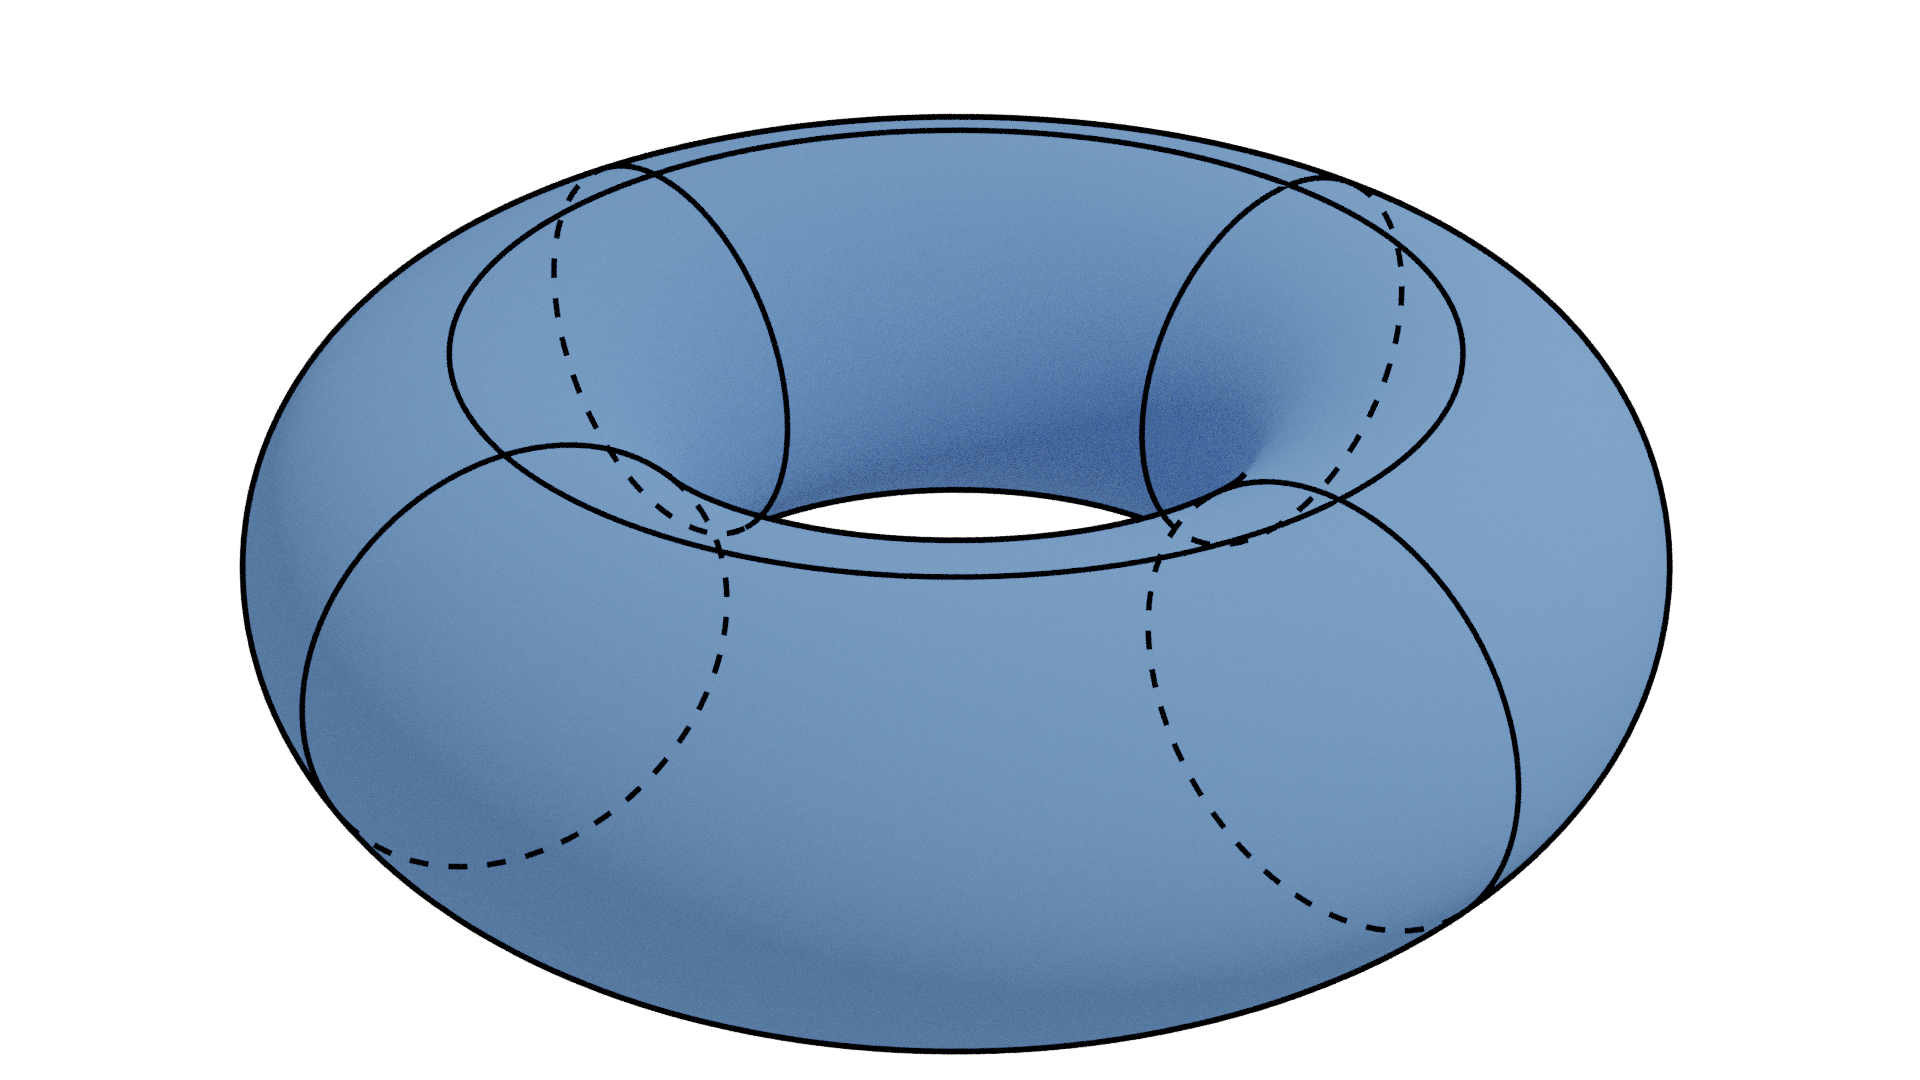
\includegraphics[width=0.3\linewidth]{Blender/Long-merid.png}
        \begin{tikzpicture}[remember picture,overlay]
            \node at (0,2.5) {Longitude}
                edge [->] (-1.3,2)
            ;
            \node at (-5.5,2.5) {Meridian}
                edge [->] (-4.0,1.5)
            ;
        \end{tikzpicture}
        \caption{Longitude and meridian curves.}
        \label{fig:longmerid}
    \end{figure}
    \item \textbf{Meridian curve}: \dq{A curve that runs once the short way around the torus}{108}
    \item \textbf{Longitude curve}: \dq{A curve that runs once around the torus the long way}{108}
    \item Every torus knot is a $(p,q)$-torus knot for some pair of positive integers $p$ and $q$.
    \begin{itemize}
        \item $p$ and $q$ will always be \textbf{relatively prime}.
    \end{itemize}
    \item \textbf{Relatively prime} (numbers): Two numbers whose greatest common divisor is $1$.
    \item On the trefoil's torus notation.
    \begin{itemize}
        \item Since the trefoil knot crosses a longitude 3 times, it must wrap around the torus thrice meridionally.
        \item Since the trefoil knot crosses a meridian 2 times, it must wrap around the torus twice longitudinally.
        \item Therefore, the trefoil knot is a $(3,2)$-torus knot.
    \end{itemize}
    \item \emph{Exercise 5.1}: What torus knot is shown in Figure \ref{fig:ex5-1}?
    \begin{figure}[h!]
        \centering
        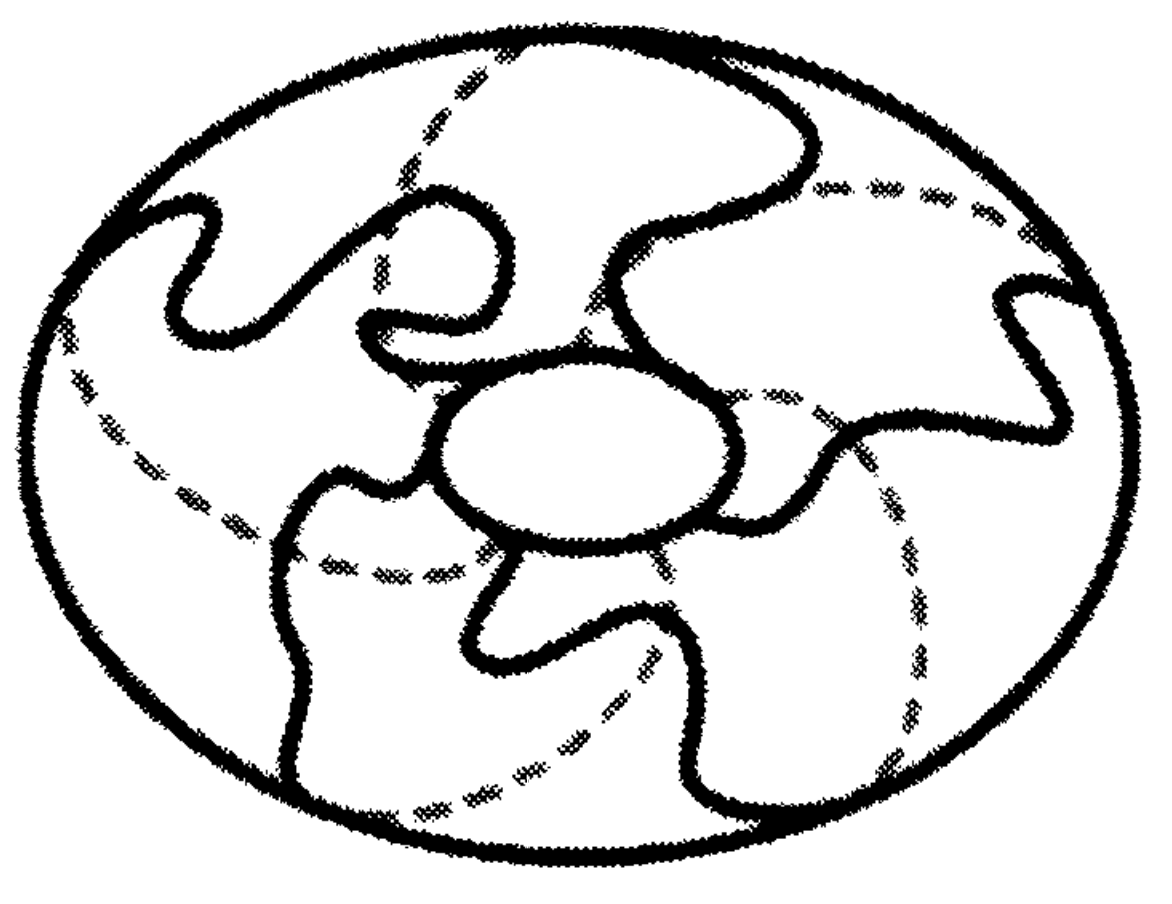
\includegraphics[width=0.2\linewidth]{Blender/ex5-1.png}
        \caption{A mystery torus knot.}
        \label{fig:ex5-1}
    \end{figure}
    \begin{itemize}
        \item Since it crosses a longitude curve five times and a meridian curve twice, it is the $(5,2)$-torus knot.
    \end{itemize}
    \item Drawing a $(p,q)$-torus knot.
    \begin{itemize}
        \item Begin by drawing two concentric ovals that represent the inner and outer bounds of the torus.
        \item Draw $p$ evenly spaced dots around the perimiter of both circles in corresponding locations.
        \item Draw a dashed, curved$^[$\footnote{Draw it curved to highlight the roundness of the torus.}$^]$ line between each corresponding point. This makes it so that the upper lines can account for all $q$ intersections with meridians.
        \item Draw a curved line between a point on the outer circle and a point that is a $\frac{q}{p}$ clockwise turn away on the inner circle.
        \item Do this for all points.
    \end{itemize}
    \item \emph{Exercise 5.2}: Draw a $(4,3)$-torus knot.
    \begin{figure}[h!]
        \centering
        \begin{tikzpicture}[
            every path/.style={thick}
            % cmark/.style={decoration={markings,
            %     mark=at position #1 with {\fill circle (2pt);}
            %     },postaction={decorate}
            % }
        ]
            \colorlet{blx}{blue}
            \colorlet{bly}{blx!10}
            \colorlet{rex}{red}
    
            \foreach \r/\c in {1/bly,0.3/white} {
                \fill [\c,scale=\r] ellipse (2cm and 1.4cm);
            }
            \foreach \r in {0,90,180,270} {
                \draw [rex,dashed,yscale=0.7,rotate=\r] (0,2) to[bend right=30] (0,0.6);
                \draw [rex,domain=-1*pi:0.5*pi,samples=500,yscale=0.7,rotate=\r] plot ({deg(\x)}:{0.6+2.8/(3*pi)*(\x+pi)});
            }
            \foreach \s in {1,0.3} {
                \draw [blue,thick,scale=\s,decoration={markings,
                    mark=between positions 0 and 0.9 step 0.25 with {\fill circle (2pt);}
                },postaction={decorate}] ellipse (2cm and 1.4cm);
                % cmark/.list={0,0.25,0.5,0.75}
            }
        \end{tikzpicture}
        \caption{Solution to \emph{Exercise 5.2}.}
        \label{fig:ex5-2}
    \end{figure}
    \item \emph{Exercise 5.3}: What would happen if we tried to draw a torus knot where $p$ and $q$ were not relatively prime? Say a $(3,6)$-torus knot?
    \begin{itemize}
        \item If $p$ and $q$ are not relatively prime, then there is some natural number $n$ that, multiplied by either $p$ or $q$ will yield the other.
        \item Thus, such a torus knot can be denoted as a $(p,np)$-torus knot or as an $(nq,q)$-torus knot where $n\in\mathbb{N}$.
        \item Let's take this case by case for each of the two above cases.
        \item Case 1: What knot is a $(p,np)$-torus knot?
        \begin{itemize}
            \item By the previously given method of drawing a knot, each point on the outer ellipse is connected with a point on the inner ellipse via a $\frac{q}{p}$ clockwise turn.
            \item If $np=q$, then such points are connected via $\frac{np}{p}=n$ clockwise turns.
            \item Thus, the point connected to via the line on the underside of the torus will be the original point.
            \item Because the strand has only completed one loop the short way around the torus, it is a meridian, and, thus, the unknot.
            \item Since this process is repeated $p$ times, a $(p,np)$-torus knot is $p$ unknots.
        \end{itemize}
        \item Case 2: What knot is an $(nq,q)$-torus knot?
        \begin{itemize}
            \item By the previously given method of drawing a knot, each point on the outer ellipse is connected with a point on the inner ellipse via a $\frac{q}{p}$ clockwise turn.
            \item If $nq=p$, then such points are connected via a $\frac{q}{nq}=\frac{1}{n}$ clockwise turn.
            \item To get back to either the original point will require 1 full turn, or $n$ turns of value $\frac{1}{n}$ (because $n\times\frac{1}{n}=1$).
            \item This process can be repeated $q$ times to yield $q$ such loops.
            \item Since these loops are the same distance apart everywhere on the torus (parallel) and have no intersections, they are a set of deformed, radially stacked unknots.
            \item Therefore, an $(nq,q)$-torus is $q$ unknots.
        \end{itemize}
        \item Therefore, a torus knot where $p$ and $q$ are not relatively prime yields a number of unknots equal to whichever value ($p$ or $q$) is smaller.
        \item A $(3,6)$-torus knot would be 3 unknots.
    \end{itemize}
    \item \emph{Exercise 5.4}: Show that a $(p,q)$-torus knot always has a projection with $p(q-1)$ crossings.
    \begin{itemize}
        \item There is a potential underpass every $\frac{1}{p}$ turn.
        \item In going through a $\frac{q}{p}$ turn, a strand begins at one of these potential underpasses and touches $\frac{q/p}{1/p}=q$ more underpasses.
        \item Therefore, there are $q+1$ possible crossings.
        \item However, since the beginning and end "crossings" are just continuations of a line, they are not crossings.
        \item Thus, each strand generates $q+1-2=q-1$ crossings.
        \item Therefore, for $p$ strands, the number of crossings is the product $p(q-1)$.
    \end{itemize}
    \item \dq{Every $(p,q)$-torus knot is also a $(q,p)$-torus knot}{110}
    \begin{itemize}
        \item Remove a disk from the torus that does not intersect the knot.
        \item Transform it into two attached bands.
        \item Turn each band inside out.
        \item Transform it back into a torus.
        \item Replace the disk.
    \end{itemize}
    \item In conjunction with \emph{Exercise 5.4}, this means that a $(p,q)$-torus knot has a projection with $q(p-1)$ crossings.
    \begin{itemize}
        \item Therefore, $c(K)\leq \min\left( p(q-1),q(p-1) \right)$.
        \item In fact, Murasugi (1991) recently proved that $c(K)= \min\left( p(q-1),q(p-1) \right)$.
    \end{itemize}
    \item \textbf{Solid torus}: \dq{A doughnut where we include both the interior of the doughnut as well as the surface}{112}
    \item \textbf{Core curve} (of a solid torus): \dq{The trivial knot that runs once around the center of the doughnut}{112}
    \item \textbf{Meridional disk} (of a solid torus): \dq{A disk that has a meridian curve as its boundary}{112}
    \item \emph{Exercise 5.5}: Let $K$ be a $(p,q)$-torus knot sitting on a torus that is the boundary of a solid torus. Let $J$ be the core curve at the center of the solid torus. Determine the linking number of $J$ and $K$. What if $K$ sits on the torus as a $(q,p)$-torus knot?
    \begin{figure}[h!]
        \centering
        \includegraphics[width=0.4\linewidth]{Blender/ex5-5.png}
        \caption{$p$ such regions exist in a solid torus.}
        \label{fig:ex5-5}
    \end{figure}
    \begin{itemize}
        \item For a $(p,q)$-torus knot, there are $p$ spirals inward and $p$ loops outward.
        \item The spirals always pass over the core curve while the loops always pass under the core curve.
        \item For each $p$, there exists a region similar to the one in Figure \ref{fig:ex5-5}. Each of these regions contributes $+1$ to the linking number as drawn (see Figure \ref{fig:linkingnumber}).
        \item Therefore, the linking number is $p$.
        \item If $K$ sits on the torus as a $(q,p)$-torus knot, then the linking number is $q$ by the same logic.
    \end{itemize}
    \item $u\left( (p,q)\text{-torus knot} \right)=\frac{(p-1)(q-1)}{2}$
    \item \emph{Exercise 5.7}: Show that in the speific case that $(p,q)=(3,4)$, the $(p,q)$-torus knot can be unknotted with $\frac{(p-1)(q-1)}{2}$ crossing changes.
    \begin{figure}[h!]
        \centering
        \begin{subfigure}[b]{0.3\linewidth}
            \centering
            \includegraphics[width=\linewidth]{Blender/ex5-7a.png}
            \caption{Original with orientation.}
            \label{fig:ex5-7a}
        \end{subfigure}
        \hspace{2em}
        \begin{subfigure}[b]{0.3\linewidth}
            \centering
            \includegraphics[width=\linewidth]{Blender/ex5-7b.png}
            \caption{Unknotted projection.}
            \label{fig:ex5-7b}
        \end{subfigure}
        \caption{Unknotting the $(3,4)$-torus knot.}
        \label{fig:ex5-7}
    \end{figure}
    \begin{itemize}
        \item Assign the orientation shown in Figure \ref{fig:ex5-7a} and start at the leftmost point on the outer edge of the torus.
        \item Use the method conjectured in \emph{Exercise 1.7} and described in detail in Section \ref{sss:UnknottingNumber}.
        \item This method will end up changing only $\frac{(3-1)(4-1)}{2}=3$ crossings and producing a projection of the unknot (Figure \ref{fig:ex5-7b}). Note the difference between Figures \ref{fig:ex5-7a} and \ref{fig:ex5-7b} to see which crossings were changed.
    \end{itemize}
    \item \dq{Seifert's algorithm applied to a projection [like Figure \ref{fig:ex5-2}] will yield a minimal genus Seifert surface}{113}
    \begin{itemize}
        \item Remember that both alternating knots and torus knots qualify as alternative knots, as mentioned in Section \ref{sss:GenusSeifert}.
    \end{itemize}
    \item \emph{Exercise 5.8} (a): Applying the above result, use a standard projection to determine the genus of a $(p,q)$-torus knot.
    \begin{itemize}
        \item Apply Seifert's algorithm to generate $s$ Seifert circles.
        \begin{itemize}
            \item Assign a clockwise orientation.
            \item At every crossing, the entering strand spiraling inward will merdge with the leaving strand looping outward.
            \item Likewise, the entering strand looping outward will merge with the leaving strand spiraling inward.
            \item As this process continues, eventually, there will be a distinct Seifert circle for each of $q$ crossings of a meridian.
            \item Therefore, $s=q$.
        \end{itemize}
        \item Count the number of crossings $c$.
        \begin{itemize}
            \item According to \emph{Exercise 5.4}, the standard projection of a $(p,q)$-torus knot has $p(q-1)$ crossings.
            \item Therefore, $c=p(q-1)$.
        \end{itemize}
        \item According to Equation \ref{eqn:gensei}, $g=\frac{c-s+1}{2}$.
        \item Therefore, the following holds.
        \begin{align*}
            g &=\frac{p(q-1)-q+1}{2}\\
            &=\frac{pq-p-q+1}{2}\\
            g &=\frac{(p-1)(q-1)}{2}\stepcounter{equation}\tag{\theequation}\label{eqn:genpq}
        \end{align*}
    \end{itemize}
    \item \emph{Exercise 5.8} (b): Does it matter if the projection comes from the knot represented as a $(q,p)$-torus knot rather than a $(p,q)$-torus knot?
    \begin{itemize}
        \item Substitute $p=q$ and $q=p$ into Equation \ref{eqn:genpq} and employ the commutative property of multiplication to prove that the first equation below is equal to Equation \ref{eqn:genpq}.
        \begin{align*}
            g &=\frac{(q-1)(p-1)}{2}\\
            &=\frac{(p-1)(q-1)}{2}
        \end{align*}
    \end{itemize}
    \item $s((p,p-1)\text{-torus knot})=2p$.
    \begin{itemize}
        \item $s(K)$ is the stick number of a knot $K$ (see Section \ref{sss:KnotsSticks}).
        \item Used the idea of curvature to obtain a lower bound for $p\geq 3$.
    \end{itemize}
    \item $s((p,q)\text{-torus knot})=2p$ if $p>q>\frac{p}{2}$.
    \begin{itemize}
        \item Used a variation on bridge number called superbridge number to obtain a lower bound.
    \end{itemize}
    \item \textbf{\emph{n}-braid}: A $(p,n)$-torus knot.
    \item \textbf{Torus knot} [formally]: \dq{A nontrivial knot that can be placed on the surface of a \textbf{standardly embedded} torus without crossing over or under itself on the surface}{114}
    \item \textbf{Standardly embedded} (surface): A surface that is unknotted in space.
    \item \textbf{Two-embeddable knot}: A knot \dq{that cannot be placed on a standardly embedded torus but that can be placed on a standardly embedded genus two surface}{114}
    \begin{itemize}
        \item The figure-eight knot is a two-embeddable knot.
    \end{itemize}
    \item \textbf{\emph{n}-embeddable knot}: A knot that \dq{can be placed on a genus $n$ standardly embedded surface without any crossings, but [that] cannot be placed on any standardly embedded surface of lower genus without crossings}{114}
    \item \emph{Exercise 5.9}: Determine the minimal genus standardly embedded surface that the $5_2$ knot can be embedded on, given that it is not a torus knot.
    \begin{figure}[h!]
        \centering
        \begin{subfigure}[b]{0.3\linewidth}
            \centering
            \includegraphics[width=0.65\linewidth]{Blender/ex5-9a.png}
            \caption{$5_2$ as tangles.}
            \label{fig:32knota}
        \end{subfigure}
        \begin{subfigure}[b]{0.6\linewidth}
            \centering
            \includegraphics[width=0.9\linewidth]{Blender/ex5-9b.png}
            \caption{$5_2$ as a two-embeddable knot.}
            \label{fig:32knotb}
        \end{subfigure}
        \caption{Solution to \emph{Exercise 5.9}.}
        \label{fig:32knot}
    \end{figure}
    \begin{itemize}
        \item This is far from an ideal method, but it does successfully embed the $5_2$ knot on a genus 2 surface.
        \item Begin with the Conway notation of the $5_2$ knot, namely $32$.
        \item This tells us that the knot can be drawn as the product of two elementary rational tangles (see Figure \ref{fig:32knota}).
        \item Draw a standardly embedded genus 2 surface.
        \item Draw the $2$ tangle on its left handle and the $3$ tangle on its right handle. Note that the choice of left versus right is arbitrary.
        \item Based on the red, blue, and green connections in Figure \ref{fig:32knota}, draw the corresponding connections in Figure \ref{fig:32knotb}.
        \item Since the purple connection cannot leave the torus like in Figure \ref{fig:32knota}, have it pass along the underside of the torus, directly, as in Figure \ref{fig:32knotb}. This will add 3 new crossings, but it will embed $5_2$ on a genus 2 surface.
    \end{itemize}
    \item A knot with bridge number $b$ is an $n$-embeddable knot where $n\leq b$.
    \item Any knot is an $n$-embeddable knot for some $n$.
    \item If $K$ is an $n$-embeddable knot, then the genus of $K$ is at most $n-1$$^[$\footnote{These last 3 statements all exist as provable exercises that are feasible with more time.}$^]$.
\end{itemize}


\subsection{Satellite Knots}
\begin{itemize}
    \item \textbf{Satellite knot}: The knot $K_3$ produced by taking a knot $K_1$, which resides within a solid torus, and then knotting the torus into a distinct knot $K_2$.
    \begin{itemize}
        \item $K_1$ must lie within the torus such that it hits every meridional disk and cannot be isotropied to miss any of the disks.
    \end{itemize}
    \item \textbf{Companion knot}: The knot $K_2$ in the above description.
    \begin{itemize}
        \item $K_2$ must be a nontrivial knot.
        \item The companion knot is the core curve about which $K_3$ \emph{orbits}. This is why $K_3$ is a \emph{satellite} knot.
    \end{itemize}
    \item For every satellite knot, there exists a knotted torus in the complement of the knot.
    \begin{itemize}
        \item This knotted torus is always incompressible.
    \end{itemize}
    \item \textbf{Whitehead double} (of the companion knot): A satellite knot where $K_1$ is the unknot twisted up as in Figure \ref{fig:whiteheaddouble}.
    \begin{figure}[h!]
        \centering
        \begin{tikzpicture}
            \colorlet{blx}{blue}
            \colorlet{bly}{blx!10}
            \colorlet{rex}{red}
    
            \begin{scope}[
                every path/.style={thick}
            ]
                \foreach \r/\c in {1/bly,0.3/white} {
                    \fill [\c,scale=\r] ellipse (2cm and 1.4cm);
                }
                \foreach \s in {1,0.3} {
                    \draw [blue,thick,scale=\s] ellipse (2cm and 1.4cm);
                }
            \end{scope}
            \begin{knot}[
                clip width=5,
                consider self intersections,
                ignore endpoint intersections=false,
                every strand/.append style={red,thick},
                background color={bly}
            ]
                \strand (-1.4,0)
                    to [out=90,in=90,looseness=2] (-0.9,0)
                    to [out=-90,in=-90,looseness=1.3] (1,0)
                    to [out=90,in=90,looseness=1.3] (-1.1,0)
                    to [out=-90,in=-90,looseness=2] (-1.6,0)
                    to [out=90,in=90,looseness=1.3] (1.5,0)
                    to [out=-90,in=-90,looseness=1.3] cycle
                ;
            \end{knot}
        \end{tikzpicture}
        \caption{$K_1$ of a Whitehead double.}
        \label{fig:whiteheaddouble}
    \end{figure}
    \begin{itemize}
        \item So named because $K_1$ resembles the Whitehead link (see Figure \ref{fig:WhiteheadBorromeana}).
        \item For example, if we take $K_1$ as the unknot in Figure \ref{fig:whiteheaddouble} and then knot the solid torus into a trefoil, we will have obtained a Whitehead double of the trefoil knot.
        \item If we perform a $k$-move where $k$ is even$^[$\footnote{This is equivalent to cutting open the torus along a meridional disk, twisting it some number of full revolutions, and gluing it back together.}$^]$ on the unknot in Figure \ref{fig:whiteheaddouble} and then knot the solid torus into a trefoil, we will have obtained another Whitehead double of the trefoil knot.
        \begin{itemize}
            \item Both of these Whitehead doubles have the property that if $\mathbb{R}^3$ is cut along the boundary of the knotted torus, the two pieces will be the solid torus at hand and three-space minus a solid torus knotted as $K_2$.
        \end{itemize}
    \end{itemize}
    \item \textbf{Two-strand cable} (of the companion knot): A satellite knot where $K_1$ is the unknot twisted up as in Figure \ref{fig:twostrandcable}.
    \begin{figure}[h!]
        \centering
        \begin{tikzpicture}
            \colorlet{blx}{blue}
            \colorlet{bly}{blx!10}
            \colorlet{rex}{red}
    
            \begin{scope}[
                every path/.style={thick}
            ]
                \foreach \r/\c in {1/bly,0.3/white} {
                    \fill [\c,scale=\r] ellipse (2cm and 1.4cm);
                }
                \foreach \s in {1,0.3} {
                    \draw [blue,thick,scale=\s] ellipse (2cm and 1.4cm);
                }
            \end{scope}
            \begin{knot}[
                clip width=5,
                consider self intersections,
                ignore endpoint intersections=false,
                every strand/.append style={red,thick},
                background color={bly}
            ]
                \strand ([rotate=10]-1.5,0)
                    to [out=90,in=-90] ([rotate=-10]-1,0)
                    to [out=90,in=90,in looseness=1.3] (1,0)
                    to [out=-90,in=-90,out looseness=1.3] ([rotate=10]-1,0)
                    to [out=90,in=-90] ([rotate=-10]-1.5,0)
                    to [out=90,in=90,in looseness=1.3] (1.5,0)
                    to [out=-90,in=-90,out looseness=1.3] cycle
                ;
            \end{knot}
        \end{tikzpicture}
        \caption{$K_1$ of a two-strand cable.}
        \label{fig:twostrandcable}
    \end{figure}
    \begin{itemize}
        \item Again, the two-strand cable will not be unique (even $k$-moves).
    \end{itemize}
    \item If $K_1$ has only one strand reaching longitudinally around the solid torus, then $K_3=K_1\#K_2$.
    \begin{itemize}
        \item Thus, satellite knots can be thought of as a broader category (a generalization) of composition in that all composite knots are satellite knots but not all satellite knots are composite knots.
        \item Note that in this case, the knotted torus is a swallow-follow torus.
    \end{itemize}
    \item In the same way that every composite knot can be factored into a unique set of prime knots, every satellite knot can be factored into a unique sequence of taking satellites.
    \item \emph{Exercise 5.14}: Determine how the satellite knot in Figure \ref{fig:ex5-14} was made. Identify its companion and draw it inside the solid torus before the solid torus is knotted.
    \begin{figure}[h!]
        \centering
        \includegraphics[width=0.25\linewidth]{Blender/ex5-14.png}
        \caption{A satellite knot.}
        \label{fig:ex5-14}
    \end{figure}
    \begin{itemize}
        \item I will not answer all parts of this exercise.
        \item The companion knot is the figure-eight knot, though.
        \item Furthermore, it appears to be constructed from the composition of 3 trefoil knots, several $k$-moves, and was originally an unknot similar to the one in Figure \ref{fig:whiteheaddouble}.
    \end{itemize}
    \item \textbf{Cable knot} (of the companion knot): A satellite knot where $K_1$ is a torus knot.
    \begin{itemize}
        \item Cable knots can be iterative, i.e., cables on cables on cables on torus knots.
    \end{itemize}
\end{itemize}


\subsection{Hyperbolic Knots}\label{sss:Hyperbolic}
\begin{itemize}
    \item It is suspected that the vast majority of knots are hyperbolic knots.
    \begin{itemize}
        \item By "the vast majority of an infinite set," \dq{we mean that for all of the prime knots of $n$ or fewer crossings, a certain large percentage of them are hyperbolic. As $n$ approaches $\infty$, that percentage is expected to approach 100\%}{119}
    \end{itemize}
    \item \dq{William Thurston proved in 1978 that the only knots that are not hyperbolic knots are torus knots and satellite knots}{119}
    \begin{itemize}
        \item Note that this statement includes all composite knots as satellite knots, a disputed claim.
    \end{itemize}
    \item \emph{Interesting tidbit on hyperbolic knot history}.
    \item \textbf{Hyperbolic knot}: \dq{A knot that has a complement that can be given a \textbf{metric} of constant curvature $-1$}{120}
    \item \textbf{Metric}: A method of measuring distance.
    \item \textbf{Euclidean metric}: The typical way to measure distance in three-space, i.e., through the use of Equation \ref{eqn:distance}.
    \begin{equation}\label{eqn:distance}
        d(P_0,P_1)=\sqrt{(x_1-x_0)^2+(y_1-y_0)^2+(z_1-z_0)^2}
    \end{equation}
    \item On curvature:
    \begin{itemize}
        \item A sphere has positive curvature --- at a point on the sphere, cross sections of the sphere through that point yield circles that all curve away in the same direction.
        \item A plane has zero curvature --- at a point on the plane, lines on the plane through that point are flat.
        \item A saddle has negative curvature --- at the central point, one cross section opens up while another opens down.
    \end{itemize}
    \item The Euclidian metric is a \textbf{flat metric}.
    \item \textbf{Flat metric}: A metric with curvature 0.
    \item \textbf{Hyperbolic metric}: A metric with curvature $-1$.
    \item \textbf{Hyperbolic geometry}: The geometry that results from applying a hyperbolic metric to three-space.
    \item \textbf{Hyperbolic three-space}: \dq{The simplest example of a three-dimensional space that has a hyperbolic metric}{121} \emph{Also known as} $\mathbb{H}^3$.
    \item The model of $\mathbb{H}^3$ considered herein is called the \textbf{Pointcar\'{e} model}.
    \item The points considered by this model are those of three-space inside the unit ball, or the following in set notation.
    \begin{equation}
        \mathbb{H}^3=\left\{ (x,y,z):x^2+y^2+z^2<1 \right\}
    \end{equation}
    \item On measuring distance in $\mathbb{H}^3$:
    \begin{figure}[h!]
        \centering
        \begin{tikzpicture}
            \colorlet{blx}{blue}
            \colorlet{bly}{blx!10}
            \colorlet{blz}{blx!50}
            \colorlet{grx}{green!50!black}
    
            \fill [bly] circle (1.5cm);
            \foreach \r/\n in {0/,45/-,135/,180/-} {
                \draw [thick,rotate=\r] (0,1.48) rectangle (\n0.1,1.38);
            }
    
            \begin{knot}[
                clip width=5,
                background color=bly,
                flip crossing/.list={3,4},
                every strand/.append style={thick}
            ]
                \strand [blx] (-1.5,0) arc[start angle=-180,end angle=0,x radius=1.5cm,y radius=0.5cm];
                \strand [blz,only when rendering/.style={dashed}] (-1.5,0) arc[start angle=180,end angle=0,x radius=1.5cm,y radius=0.5cm];
                \clip circle (1.5cm);
                \strand [grx] (-2.12,0) circle (1.5cm);
                \strand [grx] (0,1.5) to (0,-1.5);
            \end{knot}
    
            \draw [blx,ultra thick] circle (1.5cm);
            \fill [grx] (0,0.8) circle (2pt);
            \fill [grx] (0,-0.8) circle (2pt);
            \fill [grx] (-0.85,0.8) circle (2pt);
            \fill [grx] (-0.85,-0.8) circle (2pt);
            \node at (-0.4,0.8) {$P_1$};
            \node at (-0.4,-0.8) {$P_2$};
        \end{tikzpicture}
        \caption{Paths between points in $\mathbb{H}^3$.}
        \label{fig:H3paths}
    \end{figure}
    \begin{itemize}
        \item Refer to Figure \ref{fig:H3paths} throughout the following description.
        \item Let $P_1$ and $P_2$ be two points in $\mathbb{H}^3$.
        \item If $P_1$ and $P_2$ both line on a diameter, then define the partiular path between them to lie along that diameter.
        \item Otherwise, $P_1$ and $P_2$ lie on a circle that intersects both of them, and then the unit ball perpendicularly.
        \begin{itemize}
            \item Such a circle is called a \textbf{geodesic}.
            \item For any two points on a geodesic, the shortest distance between them also lies on the curve.
            \item Play the same role as straight lines in Euclidean space.
        \end{itemize}
        \item \dq{The shortest path in hyperbolic three-space from $P_1$ to $P_2$ is the path within the arc of a circle or vertical line from $P_1$ to $P_2$}{121}
        \begin{itemize}
            \item Call this path $w$.
        \end{itemize}
        \item To measure the distance between $P_1$ and $P_2$, use the following path integral$^[$\footnote{Perhaps a fun topic to explore at a later date.}$^]$ where $r$ is the distance to the origin.
        \begin{equation}
            d(P_1,P_2)=\int_w \frac{2}{1-r^2}\,\text{d}s
        \end{equation}
    \end{itemize}
    \item \textbf{Geodesic} (in $\mathbb{H}^3$): \dq{Any arc of a circle or diameter in $\mathbb{H}^3$ that is perpendicular to the unit sphere}{121}
    \item \dq{The angles of any triangle in hyperbolic three-space add up to less than $180^\circ$$^[$\footnote{Similar to the discussion of Non-Euclidian geometry and the parallel postulate in \emph{Journey Through Genius}.}$^]$}{122}
    \item Use tetrahedral pieces of $\mathbb{H}^3$ to obtain a hyperbolic manifold.
    \begin{itemize}
        \item The edges of such tetrahedra are geodesics, and the faces are geodesic planes (instead of the circular intersection in Figure \ref{fig:H3paths}, use a sphere that satisfies the same conditions).
    \end{itemize}
    \item Similar to gluing together triangles (Figure \ref{fig:triangleintersects}) to form surfaces, glue together tetrahedra in $\mathbb{H}^3$ to form a knot complement.
    \begin{itemize}
        \item \dq{If the tetrahedra that we glue together are actually hyperbolic tetrahedra, in that they sit inside hyperbolic space, and if we glue them together along their faces so that their faces match without distortion, in order that the hyperbolic method of measuring distances within the individual tetrahedra match, the result is a hyperbolic knot complement}{123}
    \end{itemize}
    \item We can then extrapolate the distance metric of $\mathbb{H}^3$ (applicable to the edges of a tetrahedron) to measure the entire knot complement hyperbolically.
    \item If this can be done, then the knot is a hyperbolic knot.
    \item The measurements facilitated by this process allow for the calculation of the \textbf{hyperbolic volume}.
    \item \textbf{Hyperbolic volume}: A positive real number that is \dq{the sum of the volumes of the individual hyperbolic tetrahedra that make up the knot complement}{123}
    \begin{itemize}
        \item Although a knot complement might seem like it's infinite, measured hyperbolically, it's finite.
    \end{itemize}
    \item Hyperbolic volume is a knot invariant.
    \begin{itemize}
        \item In fact, it is incredibly useful in distinguishing knots.
        \item However, it obviously cannot distinguish knots that are not hyperbolic.
        \item It struggles with $k$-moves sometimes.
        \item Mutants have the same hyperbolic volume.
    \end{itemize}
    \item The figure-eight knot does, indeed, have the smallest hyperbolic volume (Meyerhoff and Cao, 1997).
    \item To compute the hyperbolic volume (very surface-level):
    \begin{itemize}
        \item Cut the complement into tetrahedra.
        \item Place the tetrahedra in hyperbolic three=space.
        \item In order to ensure that they properly mesh in $\mathbb{H}^3$, a set of polynomial equations must be satisfied.
        \begin{itemize}
            \item \dq{If there are $n$ tetrahedra, we obtain $n$ polynomial equations in $n$ variables}{125}
            \item These variables are complex variables.
        \end{itemize}
        \item Use numerical methods to solve the system.
        \item The solution determines the hyperbolic metric on each tetrahedron.
        \item The volume can then be computed for each tetrahedron individually.
        \item The individual volumes can be summed to get the hyperbolic volume.
    \end{itemize}
    \item This process can be carried out by hand, but there is also a computer program to do it.
\end{itemize}


\subsection{Braids}
\begin{itemize}
    \item \textbf{Braid}: \dq{A set of $n$ strings, all of which are attached to a horizontal bar at the top and at the bottom}{127}
    \begin{itemize}
        \item See Figure \ref{fig:braidclosurea}.
    \end{itemize}
    \item Each strand can intersect a horizontal plane between the horizontal bars only once.
    \begin{itemize}
        \item Each strand must constantly head down --- it cannot loop back upward.
    \end{itemize}
    \item \textbf{Equivalent} (braids): Two braids such that one can be rearranged to look like the other \dq{without passing any strings through one another or themselves while keeping the bars fixed and keeping the strings attached to the bars}{128}
    \begin{itemize}
        \item The strings cannot be pulled over the upper bar or beneath the bottom bar in rearranging a braid.
        \item Think of the bars as infinite sheets to discourage this urge.
    \end{itemize}
    \begin{figure}[h!]
        \centering
        \begin{subfigure}[b]{0.3\linewidth}
            \centering
            \begin{tikzpicture}
                \begin{knot}[
                    clip width=5,
                    clip radius=3pt,
                    every strand/.append style={red,thick},
                    flip crossing/.list={2,4,5}
                ]
                    \strand (-0.4,1.7)
                        to [out=-90,in=90] (0,0)
                        to [out=-90,in=90] (-0.4,-0.7)
                        to [out=-90,in=90] (0.4,-1.7)
                    ;
                    \strand (0,1.7)
                        to [out=-90,in=90] (0.4,0.7)
                        to [out=-90,in=90] (-0.4,0.1)
                        to [out=-90,in=90] (-0.1,-0.8)
                        to [out=-90,in=90] (-0.4,-1.7)
                    ;
                    \strand (0.4,1.7)
                        to [out=-90,in=90] (0,0.8)
                        to [out=-90,in=90] (0.4,0)
                        to [out=-90,in=90] (0,-1.7)
                    ;
                \end{knot}
    
                \foreach \y in {,-} {
                    \draw [thick] (-0.7,\y1.7) -- (0.7,\y1.7);
                }
            \end{tikzpicture}
            \caption{A braid.}
            \label{fig:braidclosurea}
        \end{subfigure}
        \begin{subfigure}[b]{0.3\linewidth}
            \centering
            \begin{tikzpicture}
                \begin{knot}[
                    clip width=5,
                    clip radius=2pt,
                    consider self intersections,
                    ignore endpoint intersections=false,
                    every strand/.append style={red,thick},
                    scale=0.6,
                    flip crossing/.list={2,3,6}
                ]
                    \strand (-0.4,1.7)
                        to [out=-90,in=90] (0,0)
                        to [out=-90,in=90] (-0.4,-0.7)
                        to [out=-90,in=90] (0.4,-1.7)
                        to [out=-90,in=-90,looseness=1.5] (-2.4,-1.7)
                        to (-2.4,1.7)
                        to [out=90,in=90,looseness=1.5] (0.4,1.7)
                        to [out=-90,in=90] (0,0.8)
                        to [out=-90,in=90] (0.4,0)
                        to [out=-90,in=90] (0,-1.7)
                        to [out=-90,in=-90,looseness=1.5] (-2,-1.7)
                        to (-2,1.7)
                        to [out=90,in=90,looseness=1.5] (0,1.7)
                        to [out=-90,in=90] (0.4,0.7)
                        to [out=-90,in=90] (-0.4,0.1)
                        to [out=-90,in=90] (-0.1,-0.8)
                        to [out=-90,in=90] (-0.4,-1.7)
                        to [out=-90,in=-90,looseness=1.5] (-1.6,-1.7)
                        to (-1.6,1.7)
                        to [out=90,in=90,looseness=1.5] cycle
                    ;
                \end{knot}
            \end{tikzpicture}
            \vspace{-0.5em}
            \caption{The closure of the braid.}
            \label{fig:braidclosureb}
        \end{subfigure}
        \caption{A braid and its closure.}
        \label{fig:braidclosure}
    \end{figure}
    \item \textbf{Closure} (of a braid): The link formed by pulling the bottom bar around and gluing it to the top bar.
    \begin{itemize}
        \item See the difference between the braid in Figure \ref{fig:braidclosurea} and the closure of that braid in Figure \ref{fig:braidclosureb}.
    \end{itemize}
    \item Imagine an axis perpendicular to the page through the center of Figure \ref{fig:braidclosureb}.
    \begin{itemize}
        \item The closure is wrapped around this axis.
    \end{itemize}
    \item \textbf{Closed braid representation} (of a knot): A projection where there exists \dq{a choice of orientation on the knot so that, as we traverse the knot in that direction, we always travel clockwise around the axis without any backtracking}{128}
    \item \emph{Exercise 5.16}: Draw closed braid representations of the knots in Figure \ref{fig:ex5-16}. Hint: You may want to make them out of string or an extention cord and then see if you can rearrange them to travel clockwise around a pencil. Another option is to make a choice of an axis and then start to have the knot travel around the axis clockwise. Whenever it starts to travel counterclockwise, pass that portion of the knot through the axis to fix the problem. It is recommended that you do not try to use the technique that follows this problem in order to do it.
    \begin{figure}[h!]
        \centering
        \begin{subfigure}[b]{0.2\linewidth}
            \centering
            \includegraphics[width=0.8\linewidth]{Blender/ex3-8b.png}
            \caption{$4_1$}
            \label{fig:ex5-16a}
        \end{subfigure}
        \begin{subfigure}[b]{0.2\linewidth}
            \centering
            \includegraphics[width=0.8\linewidth]{Blender/ex2-3b.png}
            \caption{$6_3$}
            \label{fig:ex5-16b}
        \end{subfigure}
        \begin{subfigure}[b]{0.2\linewidth}
            \centering
            \includegraphics[width=0.85\linewidth]{Blender/ex1-22.png}
            \caption{$7_4$}
            \label{fig:ex5-16c}
        \end{subfigure}
        \caption{Draw these knots as closed braids.}
        \label{fig:ex5-16}
    \end{figure}
    \begin{figure}[h!]
        \centering
        \begin{subfigure}[b]{0.2\linewidth}
            \centering
            \includegraphics[width=0.8\linewidth]{Blender/ex5-16-2a.png}
            \caption{$4_1$}
            \label{fig:ex5-16-2a}
        \end{subfigure}
        \begin{subfigure}[b]{0.2\linewidth}
            \centering
            \includegraphics[width=0.8\linewidth]{Blender/ex5-16-2b.png}
            \caption{$6_3$}
            \label{fig:ex5-16-2b}
        \end{subfigure}
        \caption{Solution to \emph{Exercise 5.16} (incomplete).}
        \label{fig:ex5-16-2}
    \end{figure}
    \item \dq{Every knot or link is a closed braid}{129}
    \item This was proven in 1923 by J. W. Alexander of the Alexander polynomial (see Section \ref{sse:polynomials}).
    \item Let's take a look at this proof.
    %pictures?
    \begin{itemize}
        \item This proof utilizes the idea of bridges from Section \ref{sss:Bridge}.
        \item Let $L$ be a knot or link.
        \item Assign an orientation to $L$.
        \item For each subarc (strand between crossings), choose a point along said subarc.
        \item Choose a point and label it $P_1$.
        \item Proceed along the orientation of the knot, labeling each successive point $P_i$ through $P_n$. These points will be vertices (the places where overpasses and underpasses pass through the projection plane).
        \item Notice that the strand between $P_1$ and $P_2$ is an overpass while the strand between $P_2$ and $P_3$ is an underpass. In fact, the strand between $P_{2i-1}$ and $P_{2i}$ is always an overpass while the strand between $P_{2i}$ and $P_{2i+1}$ is always an underpass.
        \item Isotope the projection so that the understrands are lined up vertically next to each other. Make sure not to add any new crossings.
        \item Let $A$ be a straight line in the projection plane that is perpendicular to each underpass.
        \item Each of the underpasses obviously cross $A$ only once, but make sure that the overpasses only cross $A$ once, too.
        \begin{itemize}
            \item Every overpass crosses $A$ an odd number of times (because one must cross at least once to move from $P_{2i-1}$ to $P_{2i}$ and any other crossings could be thought of as Type II Reidemeister moves, which add 2 crossings each time).
            \item To resolve any issues, go to the problematic overpass's second crossing of $A$ along the orientation.
            \item Push it beneath $A$, reating a new underpass, a bridge that crosses $A$ once, and a bridge that crosses $A$ two fewer times.
            \item Repeat this process for all problem areas.
        \end{itemize}
        \item For all underpasses, start at $P_{2i}$, decrease $z$ until the crossing with $A$, and then increase $z$ to intersect with $P_{2i+1}$.
        \item For all overpasses, first make sure that all strands lie over the region contained by the underpasses. If the overpasses have to cross one another, that is fine. Now, start at $P_{2i-1}$, increase $z$ until the crossing with $A$, and then decrease $z$ to intersect $P_{2i}$.
        \item The result is a closed braid with $A$ as an axis.
    \end{itemize}
    \item \textbf{Braid index}: \dq{The least number of strings in a braid corresponding to a closed braid representation of the link}{132} \emph{Also known as} $b(L)$.
    \begin{table}[h!]
        \centering
        \renewcommand{\arraystretch}{1.4}
        \begin{tabular}{|r|c|c|c|}
            \hline
            \textbf{Knot}        & unknot & $3_1$ & $4_1$\\
            \hline
            \textbf{Braid index} & 1      & 2     & 3    \\
            \hline
        \end{tabular}
        \caption{Some braid indices.}
        \label{tab:simpb-L}
    \end{table}
    \item \emph{Exercise 5.17}: Describe all of the knots and links of braid index 2.
    \begin{itemize}
        \item All of the knots and links of braid index have crossings that can be undone by a single $k$-move, i.e., all such knots and links are $k$-equivalent to the trivial link of 2 components.
        \item All such knots and links are $(k,2)$-torus knots or links.
        \item If $k$ is even, the manifold is a link of 2 components of linking number $\frac{k}{2}$.
        \item If $k$ is odd, the manifold is the $k_1$ knot (Alexander-Briggs notation).
    \end{itemize}
    \item The braid index is a link invariant.
    \begin{itemize}
        \item Upper bounds are easy to find.
        \item Lower bounds, however, are difficult to find. One way uses polynomials (see Section \ref{sse:polynomials}).
    \end{itemize}
    \item \dq{The braid index of a knot is equal to the least number of Seifert circles in any projection of the knot}{132}
    \item Given a nonsplittable link $L$ with crossing number $c(L)$ and braid index $b(L)$, Equation \ref{eqn:bLcL} holds.
    \begin{equation}\label{eqn:bLcL}
        2(b(L)-1)\leq c(L)
    \end{equation}
    \item To describe a braid, use a \textbf{word}.
    \item \textbf{Word} (for a braid): Given a braid with $n$ strings, first ensure that all crossings are at different vertical heights. Working one's way down the braid from the top, denote the $i^\text{th}$ string crossing over the $(i+1)^\text{th}$ string by $\sigma_i$ and the $i^\text{th}$ string crossing under the $(i+1)^\text{th}$ string by $\sigma_i^{-1}$. Concatenate all such notations.
    \begin{figure}[h!]
        \centering
        \begin{subfigure}[b]{0.15\linewidth}
            \centering
            \begin{tikzpicture}
                \begin{knot}[
                    clip width=5,
                    every strand/.append style={red,thick}
                ]
                    \strand (-0.4,1.7)
                        to (-0.4,0.7)
                        to [out=-90,in=90] (0,-0.7)
                        to (0,-1.7)
                    ;
                    \strand (0,1.7)
                        to (0,0.7)
                        to [out=-90,in=90] (-0.4,-0.7)
                        to (-0.4,-1.7)
                    ;
                    \strand (0.4,1.7)
                        to (0.4,-1.7)
                    ;
                \end{knot}
    
                \foreach \y in {,-} {
                    \draw [thick] (-0.7,\y1.7) -- (0.7,\y1.7);
                }
            \end{tikzpicture}
            \caption{$\sigma_1$}
            \label{fig:braidcrossingsa}
        \end{subfigure}
        \begin{subfigure}[b]{0.15\linewidth}
            \centering
            \begin{tikzpicture}
                \begin{knot}[
                    clip width=5,
                    every strand/.append style={red,thick}
                ]
                    \strand (-0.4,1.7)
                        to (-0.4,0.7)
                        to [out=-90,in=90] (0,-0.7)
                        to (0,-1.7)
                    ;
                    \strand (0,1.7)
                        to (0,0.7)
                        to [out=-90,in=90] (-0.4,-0.7)
                        to (-0.4,-1.7)
                    ;
                    \strand (0.4,1.7)
                        to (0.4,-1.7)
                    ;
                    \flipcrossings{1}
                \end{knot}
    
                \foreach \y in {,-} {
                    \draw [thick] (-0.7,\y1.7) -- (0.7,\y1.7);
                }
            \end{tikzpicture}
            \caption{$\sigma_1^{-1}$}
            \label{fig:braidcrossingsb}
        \end{subfigure}
        \begin{subfigure}[b]{0.15\linewidth}
            \centering
            \begin{tikzpicture}
                \begin{knot}[
                    clip width=5,
                    every strand/.append style={red,thick}
                ]
                    \strand (0,1.7)
                        to (0,0.7)
                        to [out=-90,in=90] (0.4,-0.7)
                        to (0.4,-1.7)
                    ;
                    \strand (0.4,1.7)
                        to (0.4,0.7)
                        to [out=-90,in=90] (0,-0.7)
                        to (0,-1.7)
                    ;
                    \strand (-0.4,1.7)
                        to (-0.4,-1.7)
                    ;
                \end{knot}
    
                \foreach \y in {,-} {
                    \draw [thick] (-0.7,\y1.7) -- (0.7,\y1.7);
                }
            \end{tikzpicture}
            \caption{$\sigma_2$}
            \label{fig:braidcrossingsc}
        \end{subfigure}
        \begin{subfigure}[b]{0.15\linewidth}
            \centering
            \begin{tikzpicture}
                \begin{knot}[
                    clip width=5,
                    every strand/.append style={red,thick}
                ]
                    \strand (0,1.7)
                        to (0,0.7)
                        to [out=-90,in=90] (0.4,-0.7)
                        to (0.4,-1.7)
                    ;
                    \strand (0.4,1.7)
                        to (0.4,0.7)
                        to [out=-90,in=90] (0,-0.7)
                        to (0,-1.7)
                    ;
                    \strand (-0.4,1.7)
                        to (-0.4,-1.7)
                    ;
                    \flipcrossings{1}
                \end{knot}
    
                \foreach \y in {,-} {
                    \draw [thick] (-0.7,\y1.7) -- (0.7,\y1.7);
                }
            \end{tikzpicture}
            \caption{$\sigma_2^{-1}$}
            \label{fig:braidcrossingsd}
        \end{subfigure}
        \begin{subfigure}[b]{0.15\linewidth}
            \centering
            \begin{tikzpicture}
                \begin{knot}[
                    clip width=5,
                    every strand/.append style={red,thick}
                ]
                    \strand (-0.4,1.7)
                        to (-0.4,1.4)
                        to [out=-90,in=90] (0.4,-1.4)
                        to (0.4,-1.7)
                    ;
                    \strand (0,1.7)
                        to (0,1.4)
                        to [out=-90,in=90] (-0.4,0)
                        to (-0.4,-1.7)
                    ;
                    \strand (0.4,1.7)
                        to (0.4,0)
                        to [out=-90,in=90] (0,-1.4)
                        to (0,-1.7)
                    ;
                    \flipcrossings{2}
                \end{knot}
    
                \foreach \y in {,-} {
                    \draw [thick] (-0.7,\y1.7) -- (0.7,\y1.7);
                }
            \end{tikzpicture}
            \caption{$\sigma_1\sigma_2^{-1}$}
            \label{fig:braidcrossingse}
        \end{subfigure}
        \caption{Denoting crossings in a braid.}
        \label{fig:braidcrossings}
    \end{figure}
    \item \emph{Exercise 5.18}: Draw the five-string braid given by the word $\sigma_1\sigma_2\sigma_3\sigma_2^{-1}\sigma_4\sigma_1^{-1}$.
    \begin{figure}[h!]
        \centering
        \includegraphics[width=0.12\linewidth]{Blender/ex5-18.png}
        \caption{Solution to \emph{Exercise 5.18}.}
        \label{fig:ex5-18}
    \end{figure}
    \item \emph{Exercise 5.19}: Identify the knot that has four-string braid word $\left( \sigma_1^{-1}\sigma_2\sigma_3^{-1} \right)^2{\sigma_3}^3$. It is one of the six-crossing knots.
    \begin{itemize}
        \item After drawing the closure of the braid, reduce crossings down to six.
        \item At this point, a 4 tangle and a 2 tangle can be picked out.
        \item Therefore, this is the $6_1$ knot.
    \end{itemize}
    \item \emph{Exercise 5.20}: Find a word such that the closure of the corresponding braid gives the $6_3$ knot.
    \begin{itemize}
        \item Use Figure \ref{fig:ex5-16-2b}, which gives a closed braid representation of $6_3$. From this projection, it is possible to pick find the word.
        \item Therefore, the word is $\sigma_2\sigma_2\sigma_1^{-1}\sigma_2\sigma_1^{-1}\sigma_1^{-1}$.
    \end{itemize}
    \item \emph{Exercise 5.21}: Show that the closure of the $n$-string braid $\left( \sigma_1\sigma_2\cdots\sigma_{n-1} \right)^m$ is a knot if and only if $n$ and $m$ are relatively prime.
    \begin{itemize}
        % \item If $m=cn$ where $c\in\mathbb{N}$ for the word in question, then every strand touches the bottom and top bar at the same position relative to every other strand. Therefore, a link of $n$ components is generated.
        % \item If $n=cm$ where $c\in\mathbb{N}$ for the word in question, then every strand shifts $m$ places from top to bottom. Therefore, a loop will pass through the braid $\frac{n}{m}=\frac{cm}{m}=c$ times before reaching its starting point. Therefore, a link of $c$ components is generated.
        \item Given this particular word, every strand "shifts" $m$ places from top to bottom.
        \begin{itemize}
            \item Consider a scenario where $n=3$ and $m=1$.
            \item The left strand at the top becomes the rightmost strand at the bottom by the definition of the word.
            \item This means that the right strand at the top becomes the middle strand at the bottom and the middle strand at the top becomes the left strand at the bottom.
            \item Now consider when $n=3$ and $m=2$.
            \item The above shifting of strands takes place, but then it takes place again, i.e., every strand shifts twice.
            \item Thus, from top to bottom, left $\rightarrow$ right $\rightarrow$ middle, middle $\rightarrow$ left $\rightarrow$ right, and right $\rightarrow$ middle $\rightarrow$ left.
        \end{itemize}
        \item Take a strand that is $i^\text{th}$ from the left at the top.
        \item Assuming that $i>m$, the strand will be $(i-m)^\text{th}$ from the left at the bottom.
        \item Therefore, it will reenter the top of the braid in the $(i-m)^\text{th}$ from the left position.
        \item It may then leave at the $(i-2m)^\text{th}$ from the left position (or it may shift back to the right side).
        \item Regardless, it will pass through some number of strands of the braid in this fashion.
        \item Only if $n$ and $m$ are relatively prime will one loop pass through every strand in a nontrivial fashion.
    \end{itemize}
    \item \emph{Exercise 5.22}: Check that the closure of the $n$-string braid $\left( \sigma_1\sigma_2\cdots\sigma_{n-1} \right)^m$ is simply the $(m,n)$-torus knot (assuming $m$ and $n$ are relatively prime).
    \begin{itemize}
        \item Indeed, this is the case.
    \end{itemize}
    \item The word notation has some useful advantages.
    \begin{figure}[h!]
        \centering
        \begin{subfigure}[b]{0.15\linewidth}
            \centering
            \begin{tikzpicture}
                \begin{knot}[
                    clip width=5,
                    every strand/.append style={red,thick}
                ]
                    \strand (0,1.7)
                        to (0,-1.7)
                    ;
                    \strand (-0.4,1.7)
                        to (-0.4,-1.7)
                    ;
                    \strand (0.4,1.7)
                        to (0.4,-1.7)
                    ;
                    \strand (-0.8,1.7)
                        to (-0.8,-1.7)
                    ;
                \end{knot}
        
                \foreach \y in {,-} {
                    \draw [thick] (-1.1,\y1.7) -- (0.7,\y1.7);
                }
            \end{tikzpicture}
            \caption{$1$}
            \label{fig:braidIIa}
        \end{subfigure}
        \begin{subfigure}[b]{0.15\linewidth}
            \centering
            \begin{tikzpicture}
                \begin{knot}[
                    clip width=5,
                    every strand/.append style={red,thick}
                ]
                    \strand (-0.4,1.7)
                        to [out=-90,in=90] (0,0)
                        to [out=-90,in=90] (-0.4,-1.7)
                    ;
                    \strand (0,1.7)
                        to [out=-90,in=90] (-0.4,0)
                        to [out=-90,in=90] (0,-1.7)
                    ;
                    \strand (0.4,1.7)
                        to (0.4,-1.7)
                    ;
                    \strand (-0.8,1.7)
                        to (-0.8,-1.7)
                    ;
                \end{knot}
        
                \foreach \y in {,-} {
                    \draw [thick] (-1.1,\y1.7) -- (0.7,\y1.7);
                }
            \end{tikzpicture}
            \caption{$\sigma_i\sigma_i^{-1}$}
            \label{fig:braidIIb}
        \end{subfigure}
        \caption{Braids equivalent via a Type II Reidemeister move.}
        \label{fig:braidII}
    \end{figure}
    \begin{itemize}
        \item If a $\sigma_i\sigma_i^{-1}$ term appears somewhere within a word, it corresponds to the crossings shown in Figure \ref{fig:braidII}.
        \item These crossings can easily be undone via a Type II Reidemesiter move.
        \item In the same way, $\sigma_i\sigma_i^{-1}=1$ by the definition of an inverse, so the term reduces out of the word.
    \end{itemize}
    \item \emph{Exercise 5.23}: If a given word represents a knot with a particular orientation, what word gives the same knot but with the opposite orientation?
    \begin{itemize}
        \item Take the terms of the word and reverse their order.
    \end{itemize}
    \item To multiply two $n$-string braids, just stack them on top of each other.
    \begin{itemize}
        \item This is reflected by the notation --- stacking tangles means that the word of the top one will be immediately followed by the word of the bottom one.
    \end{itemize}
    \item \emph{Exercise 5.24} (a): Describe an $n$-string braid $I_n$ that acts as an identify when it multiplies any other $n$-string braid. That is to say, multiplying a braid $B$ by this braid yields the braid $B$ back again.
    \begin{itemize}
        \item $I_n$ is the trivial braid of $n$-strings.
        \item Multiplication extends the bottom strands, but they can be isotoped back to being shorter.
    \end{itemize}
    \item \emph{Exercise 5.24} (b): Describe an inverse braid for a given braid $B$. That is to say, find a braid $B^{-1}$ that has the property that $BB^{-1}=I_n=B^{-1}B$.
    \begin{itemize}
        \item $B^{-1}$ is just $B$ but with the inverse of the terms of the word listed in reverse order.
        \item For example, if $B=\sigma_1\sigma_2^{-1}\sigma_2$, then $B^{-1}=\sigma_2^{-1}\sigma_2\sigma_1^{-1}$.
    \end{itemize}
    \item \emph{Exercise 5.24} (c): Show that the multiplication of $n$-string braids is associative, namely $B_1\left( B_2B_3 \right)=\left( B_1B_2 \right)B_3$ for any threee $n$-string braids $B_1$, $B_2$, and $B_3$.
    \begin{itemize}
        \item Since the terms of a word follow the normal rules of multiplication, so do words, themselves$^[$\footnote{This is like proving that a vector space is closed under addition and scalar multiplication using the fact the regular numbers (components of vectors) are obey addition and scalar multiplication.}$^]$.
    \end{itemize}
    \item $B_n$ will denote the \textbf{group} of $n$-string braids (developed throughout \emph{Exercise 5.24}).
    \item \textbf{Group}: A set of elements and a way to multiply the elements such that:
    \begin{enumerate}
        \item \dq{There exists an identity element that, when multiplying any element, doesn't change it;
        \item Every element has an inverse;
        \item The multiplication is associative, that is, $a(bc)=(ab)c$ for any three elements $a$, $b$, and $c$ of the group}{135}
    \end{enumerate}
    \item A particular element of $B_n$ is an equivalent class of braids.
    \item \emph{Exercise 5.26}: Using a picture, show that the two braids $\sigma_i\sigma_{i+1}\sigma_i$ and $\sigma_{i+1}\sigma_i\sigma_{i+1}$ are equivalent.
    \begin{figure}[h!]
        \centering
        \begin{subfigure}[b]{0.2\linewidth}
            \centering
            \begin{tikzpicture}
                \begin{knot}[
                    clip width=5,
                    every strand/.append style={red,thick}
                ]
                    \strand (-0.4,1.7)
                        to (-0.4,1.2)
                        to [out=-90,in=90] (0.4,-0.4)
                        to (0.4,-1.7)
                    ;
                    \strand (0,1.7)
                        to (0,1.2)
                        to [out=-90,in=90] (-0.4,0.4)
                        to (-0.4,-0.4)
                        to [out=-90,in=90] (0,-1.2)
                        to (0,-1.7)
                    ;
                    \strand (0.4,1.7)
                        to (0.4,0.4)
                        to [out=-90,in=90] (-0.4,-1.2)
                        to (-0.4,-1.7)
                    ;
                    \strand (0.8,1.7)
                        to (0.8,-1.7)
                    ;
                    \strand (-0.8,1.7)
                        to (-0.8,-1.7)
                    ;
                \end{knot}
        
                \foreach \y in {,-} {
                    \draw [thick] (-1.1,\y1.7) -- (1.1,\y1.7);
                }
            \end{tikzpicture}
            \caption{$\sigma_i\sigma_{i+1}\sigma_i$}
            \label{fig:braidIIIa}
        \end{subfigure}
        \begin{subfigure}[b]{0.2\linewidth}
            \centering
            \begin{tikzpicture}
                \begin{knot}[
                    clip width=5,
                    every strand/.append style={red,thick}
                ]
                    \strand [rotate=180] (-0.4,1.7)
                        to (-0.4,1.2)
                        to [out=-90,in=90] (0.4,-0.4)
                        to (0.4,-1.7)
                    ;
                    \strand [rotate=180] (0,1.7)
                        to (0,1.2)
                        to [out=-90,in=90] (-0.4,0.4)
                        to (-0.4,-0.4)
                        to [out=-90,in=90] (0,-1.2)
                        to (0,-1.7)
                    ;
                    \strand [rotate=180] (0.4,1.7)
                        to (0.4,0.4)
                        to [out=-90,in=90] (-0.4,-1.2)
                        to (-0.4,-1.7)
                    ;
                    \strand (0.8,1.7)
                        to (0.8,-1.7)
                    ;
                    \strand (-0.8,1.7)
                        to (-0.8,-1.7)
                    ;
                \end{knot}
        
                \foreach \y in {,-} {
                    \draw [thick] (-1.1,\y1.7) -- (1.1,\y1.7);
                }
            \end{tikzpicture}
            \caption{$\sigma_{i+1}\sigma_i\sigma_{i+1}$}
            \label{fig:braidIIIb}
        \end{subfigure}
        \caption{Braids equivalent via a Type III Reidemeister move.}
        \label{fig:braidIII}
    \end{figure}
    \item If $\sigma_i\sigma_j$ is changed to $\sigma_j\sigma_i$ when $|i-j|>1$, equivalence is maintained.
    \begin{figure}[h!]
        \centering
        \begin{subfigure}[b]{0.25\linewidth}
            \centering
            \begin{tikzpicture}
                \begin{knot}[
                    clip width=5,
                    every strand/.append style={red,thick}
                ]
                    \strand (0.4,1.7)
                        to (0.4,0)
                        to [out=-90,in=90] (0.8,-1.4)
                        to (0.8,-1.7)
                    ;
                    \strand (0.8,1.7)
                        to (0.8,0)
                        to [out=-90,in=90] (0.4,-1.4)
                        to (0.4,-1.7)
                    ;
                    \strand [rotate=180] (0.4,1.7)
                        to (0.4,0)
                        to [out=-90,in=90] (0.8,-1.4)
                        to (0.8,-1.7)
                    ;
                    \strand [rotate=180] (0.8,1.7)
                        to (0.8,0)
                        to [out=-90,in=90] (0.4,-1.4)
                        to (0.4,-1.7)
                    ;
                    \strand (0,1.7)
                        to (0,-1.7)
                    ;
                    \strand (1.2,1.7)
                        to (1.2,-1.7)
                    ;
                    \strand (-1.2,1.7)
                        to (-1.2,-1.7)
                    ;
                \end{knot}
        
                \foreach \y in {,-} {
                    \draw [thick] (-1.5,\y1.7) -- (1.5,\y1.7);
                }
            \end{tikzpicture}
            \caption{$\sigma_i\sigma_j$}
            \label{fig:braid121a}
        \end{subfigure}
        \begin{subfigure}[b]{0.25\linewidth}
            \centering
            \begin{tikzpicture}
                \begin{knot}[
                    clip width=5,
                    every strand/.append style={red,thick}
                ]
                    \strand (0.4,1.7)
                        to (0.4,1.4)
                        to [out=-90,in=90] (0.8,0)
                        to (0.8,-1.7)
                    ;
                    \strand (0.8,1.7)
                        to (0.8,1.4)
                        to [out=-90,in=90] (0.4,0)
                        to (0.4,-1.7)
                    ;
                    \strand [rotate=180] (0.4,1.7)
                        to (0.4,1.4)
                        to [out=-90,in=90] (0.8,0)
                        to (0.8,-1.7)
                    ;
                    \strand [rotate=180] (0.8,1.7)
                        to (0.8,1.4)
                        to [out=-90,in=90] (0.4,0)
                        to (0.4,-1.7)
                    ;
                    \strand (0,1.7)
                        to (0,-1.7)
                    ;
                    \strand (1.2,1.7)
                        to (1.2,-1.7)
                    ;
                    \strand (-1.2,1.7)
                        to (-1.2,-1.7)
                    ;
                \end{knot}
        
                \foreach \y in {,-} {
                    \draw [thick] (-1.5,\y1.7) -- (1.5,\y1.7);
                }
            \end{tikzpicture}
            \caption{$\sigma_j\sigma_i$}
            \label{fig:braid121b}
        \end{subfigure}
        \caption{Braids equivalent via a shifting of unconnected strings.}
        \label{fig:braid121}
    \end{figure}
    \begin{itemize}
        \item Not based on a Type I Reidemeister move.
        \item Just changes the relative height of two distinct twists.
    \end{itemize}
    \item \dq{Two words $w_1$ and $w_2$ represent the same braid if and only if we can get from the one word to the other by a sequence of these operations}{136}
    \item \emph{Exercise 5.27}: Show that the two words $w_1=\sigma_2\sigma_1\sigma_2\sigma_1\sigma_2^{-1}\sigma_4$ and $w_2={\sigma_2}^2\sigma_3\sigma_1\sigma_3^{-1}\sigma_4$ represent the same five-string braid, up to equivalence.
    \begin{align*}
        w_1 =&\ \sigma_2\sigma_1\sigma_2\sigma_1\sigma_2^{-1}\sigma_4\\
        \xrightarrow{\text{Rule 2}} &\ \sigma_2\sigma_2\sigma_1\sigma_2\sigma_2^{-1}\sigma_4\\
        \xrightarrow{\text{Rule 1}} &\ \sigma_2\sigma_2\sigma_1\sigma_4\\
        \xrightarrow{\text{Condense}} &\ {\sigma_2}^2\sigma_1\sigma_4\\
        \xrightarrow{\text{Rule 1}} &\ {\sigma_2}^2\sigma_1\sigma_3\sigma_3^{-1}\sigma_4\\
        \xrightarrow{\text{Rule 3}} &\ {\sigma_2}^2\sigma_3\sigma_1\sigma_3^{-1}\sigma_4=w_2
    \end{align*}
    \item \textbf{Markov equivalent} (braids): Two braids whose \dq{closures yield the same oriented link}{137}
    \item \textbf{Markov's theorem}: Two braids are Markov equivalent if and only if they can be transformed into one another via the previous three operations, \textbf{conjugation}, and \textbf{stabilization}.
    \item \textbf{Conjugation}: Multiply the word by $\sigma_j$ at the beginning and $\sigma_j^{-1}$ at the end (or vice versa).
    \begin{figure}[h!]
        \centering
        \begin{subfigure}[b]{0.2\linewidth}
            \centering
            \begin{tikzpicture}
                \begin{knot}[
                    clip width=5,
                    every strand/.append style={red,thick}
                ]
                    \strand (0,1.7)
                        to (0,-1.7)
                    ;
                    \strand (-0.4,1.7)
                        to (-0.4,-1.7)
                    ;
                    \strand (0.4,1.7)
                        to (0.4,-1.7)
                    ;
                    \strand (-0.8,1.7)
                        to (-0.8,-1.7)
                    ;
                \end{knot}
    
                \node [draw=red,thick,fill=white,minimum width=1.4cm] at (-0.2,0) {Braid};
        
                \foreach \y in {,-} {
                    \draw [thick] (-1.1,\y1.7) -- (0.7,\y1.7);
                }
            \end{tikzpicture}
            \caption{Unconjugated.}
            \label{fig:braidII2a}
        \end{subfigure}
        \begin{subfigure}[b]{0.2\linewidth}
            \centering
            \begin{tikzpicture}
                \begin{knot}[
                    clip width=5,
                    every strand/.append style={red,thick}
                ]
                    \strand (-0.4,1.7)
                        to [out=-90,in=90] (0,0)
                        to [out=-90,in=90] (-0.4,-1.7)
                    ;
                    \strand (0,1.7)
                        to [out=-90,in=90] (-0.4,0)
                        to [out=-90,in=90] (0,-1.7)
                    ;
                    \strand (0.4,1.7)
                        to (0.4,-1.7)
                    ;
                    \strand (-0.8,1.7)
                        to (-0.8,-1.7)
                    ;
                \end{knot}
    
                \node [draw=red,thick,fill=white,minimum width=1.4cm] at (-0.2,0) {Braid};
        
                \foreach \y in {,-} {
                    \draw [thick] (-1.1,\y1.7) -- (0.7,\y1.7);
                }
            \end{tikzpicture}
            \caption{Conjugated.}
            \label{fig:braidII2b}
        \end{subfigure}
        \caption{Braids equivalent via conjugation by $\sigma_j$.}
        \label{fig:braidII2}
    \end{figure}
    \item \textbf{Stabilization}: Multiply the word $w$ corresponding to an $n$-string braid by $\sigma_n$ to yield $w\sigma_n$. Alternatively, given an $(n+1)$-string braid $w\sigma_n$ where $\sigma_n$ is only present as the last term, remove $\sigma_n$ to yield $w$. Multiplying by or removing $\sigma_n^{-1}$ is also valid.
    \begin{figure}[h!]
        \centering
        \begin{subfigure}[b]{0.2\linewidth}
            \centering
            \begin{tikzpicture}
                \begin{knot}[
                    clip width=5,
                    every strand/.append style={red,thick}
                ]
                    \strand (0,1.7)
                        to (0,-1.7)
                    ;
                    \strand (-0.4,1.7)
                        to (-0.4,-1.7)
                    ;
                    \strand (0.4,1.7)
                        to (0.4,-1.7)
                    ;
                    \strand (-0.8,1.7)
                        to (-0.8,-1.7)
                    ;
                \end{knot}
    
                \node [draw=red,thick,fill=white,minimum width=1.4cm] at (-0.2,0) {Braid};
        
                \foreach \y in {,-} {
                    \draw [thick] (-1.1,\y1.7) -- (0.7,\y1.7);
                }
            \end{tikzpicture}
            \caption{$n$-strings.}
            \label{fig:braidIa}
        \end{subfigure}
        \begin{subfigure}[b]{0.2\linewidth}
            \centering
            \begin{tikzpicture}
                \begin{knot}[
                    clip width=5,
                    every strand/.append style={red,thick}
                ]
                    \strand (0.4,1.7)
                        to (0.4,0)
                        to [out=-90,in=90] (0.8,-1.7)
                    ;
                    \strand (0.8,1.7)
                        to (0.8,0)
                        to [out=-90,in=90] (0.4,-1.7)
                    ;
                    \strand (0,1.7)
                        to (0,-1.7)
                    ;
                    \strand (-0.4,1.7)
                        to (-0.4,-1.7)
                    ;
                    \strand (-0.8,1.7)
                        to (-0.8,-1.7)
                    ;
                \end{knot}
    
                \node [draw=red,thick,fill=white,minimum width=1.4cm] at (-0.2,0) {Braid};
        
                \foreach \y in {,-} {
                    \draw [thick] (-1.1,\y1.7) -- (0.7,\y1.7);
                }
            \end{tikzpicture}
            \caption{$(n+1)$-strings.}
            \label{fig:braidIb}
        \end{subfigure}
        \begin{subfigure}[b]{0.2\linewidth}
            \centering
            \begin{tikzpicture}
                \begin{knot}[
                    clip width=5,
                    consider self intersections,
                    every strand/.append style={red,thick}
                ]
                    \strand (0.4,1.7)
                        to [out=-90,in=90] (0.4,0)
                        to [out=-90,in=90] (0.8,-1.4)
                        to [out=-90,in=-90,looseness=1.8] (1.2,-1.4)
                        to (1.2,1.4)
                        to [out=90,in=90,looseness=1.8] (0.8,1.4)
                        to [out=-90,in=90] (0.8,0)
                        to [out=-90,in=90] (0.4,-1.7)
                    ;
                    \strand (0,1.7)
                        to (0,-1.7)
                    ;
                    \strand (-0.4,1.7)
                        to (-0.4,-1.7)
                    ;
                    \strand (-0.8,1.7)
                        to (-0.8,-1.7)
                    ;
                \end{knot}
    
                \node [draw=red,thick,fill=white,minimum width=1.4cm] at (-0.2,0) {Braid};
        
                \foreach \y in {,-} {
                    \draw [thick] (-1.1,\y1.7) -- (0.7,\y1.7);
                }
            \end{tikzpicture}
            \caption{Showing the loop.}
            \label{fig:braidIc}
        \end{subfigure}
        \caption{Braids equivalent via stabilization by $\sigma_n$.}
        \label{fig:braidI}
    \end{figure}
    \begin{itemize}
        \item This move changes the number of strings/loops in a closed braid.
        \item It is kind of like a Type I Reidemeister move.
    \end{itemize}
    \item \textbf{Letter}: An individual $\sigma_i^{\pm 1}$ term in a word.
    \item \textbf{Markov moves}: Formally, the five listed operations (Figures \ref{fig:braidII}, \ref{fig:braidIII}, \ref{fig:braid121}, \ref{fig:braidII2}, and \ref{fig:braidI}).
\end{itemize}


\subsection{Almost Alternating Knots}
\begin{itemize}
    \item \textbf{Almost alternating knot}: A nonalternating knot that has a projection where one crossing change would make the knot alternating.
    \item \dq{Of the 393 nonalternating knots and links of eleven or fewer crossings, all but at most three are almost alternating}{140}
    \item \dq{An algebraic knot that contains no negative signs in its Conway notation is in fact an alternating knot}{141}
    \item \dq{An algebraic link that has exactly one negative sign in its Conway notation has an almost alternating projection$^[$\footnote{Available as an exercise.}$^]$}{141}
    \begin{itemize}
        \item This statement proves that all but 17 of Conway's nonalternating knots are almost alternating.
    \end{itemize}
    \item In this section, results known for alternating knots (many are listed in Section \ref{sse:polynomials}) will be generalized to almost alternating knots.
    \item \dq{Every alternating knot or link has an almost alternating projection}{141}
    \begin{itemize}
        \item A Type II Reidemeister move on the alternating projection produces an almost alternating projection.
    \end{itemize}
    \item \dq{A prime almost alternating knot is either a torus knot or a hyperbolic knot}{142}
    \begin{itemize}
        \item Thus, no satellite knot is an almost alternating knot.
        \item This is an extention of the previously known fact that a prime alternating link is either a torus link or a hyperbolic link.
        \item Because the only alternating torus links are the closures of braids where $b(L)=2$ (see \emph{Exercise 5.17}), almost all prime alternating links are hyperbolic.
    \end{itemize}
    \item \textbf{Tongue move}: A Type II Reidemeister move followed by a Type III Reidemeister move about the nonalternating crossing$^[$\footnote{This is a Type II bridging move!}$^]$.
    \begin{figure}[h!]
        \centering
        \begin{tikzpicture}
            \colorlet{orx}{orange}
            \colorlet{ory}{orx!10}
    
            \begin{scope}[
                xshift=-3cm
            ]
                \fill [ory] (-2,-2) rectangle (2,2);
                \node at (0,-1.7) {Alternating out here};
                \filldraw [draw=red,thick,fill=white] circle (1cm);
                \begin{knot}[
                    clip width=5,
                    clip radius=3pt,
                    ignore endpoint intersections=false,
                    every strand/.append style={red,thick}
                ]
                    \clip circle (1cm);
                    \strand (-1,0) to (1,0);
                    \strand (0,-1) to (0,1);
                    \strand (-1.6,0) circle (1cm);
                    \strand (1.6,0) circle (1cm);
                    \strand (0,-1.6) circle (1cm);
                    \strand (0,1.6) circle (1cm);
                    \flipcrossings{1,2,3}
                \end{knot}
                \draw [cyan,thick,dashed,dash pattern=on 2pt off 1pt,dash phase=1pt] circle (2mm);
            \end{scope}
            \draw [very thick,-latex] (-0.4,0) -- (0.4,0);
            \begin{scope}[
                xshift=3cm
            ]
                \fill [ory] (-2,-2) rectangle (2,2);
                \node at (0,-1.7) {Alternating out here};
                \filldraw [draw=red,thick,fill=white] circle (1cm);
                \begin{knot}[
                    clip width=5,
                    clip radius=3pt,
                    ignore endpoint intersections=false,
                    every strand/.append style={red,thick}
                ]
                    \clip circle (1cm);
                    \strand (-1,0) to (1,0);
                    \strand (0,-1) to (0,1);
                    \strand (-1.6,0) circle (1cm);
                    \strand (1.6,0) circle (1cm);
                    \strand (-0.6,-0.8)
                        to [out=30,in=180] (0,0.3)
                        to [out=0,in=150] (0.6,-0.8)
                    ;
                    \strand (0,1.6) circle (1cm);
                    \flipcrossings{1,2,3}
                \end{knot}
                \draw [cyan,thick,dashed,dash pattern=on 2pt off 1pt,dash phase=1pt] (0,0.3) circle (2mm);
            \end{scope}
        \end{tikzpicture}
        \caption{A tongue move.}
        \label{fig:tongue}
    \end{figure}
    \item \textbf{\emph{m}-almost alternating knot}: \dq{A knot that has a projection where $m$ crossing changes would make the projection alternating, and the knot has no projection that could be made alternating in fewer crossing changes}{144}
    \begin{itemize}
        \item Alternating knots are $0$-almost alternating knots and almost alternating knots are $1$-almost alternating knots.
    \end{itemize}
    \item The simplest Whitehead double of the trefoil knot is $2$-almost alternating.
    \begin{itemize}
        \item It is not alternating.
        \item It is a satellite knot, and, thus, is not almost alternating.
        \item There exists a projection of it where two crossing changes would make it alternating.
    \end{itemize}
    \item \emph{Exercise 5.33}: Show that every knot is $m$-almost alternating for some $m$.
    \begin{itemize}
        \item Take a projection of a knot.
        \item Assign an orientation.
        \item Choose a crossing from which to begin traversing the knot.
        \item Leave on the understrand.
        \item If the next crossing is not passed through on the overstrand, flip the crossing. Otherwise, continue along.
        \item If the crossing after that is not passed through on the understrand, flip the crossing. Otherwise, continue along.
        \item Continue in this manner until you arrive at the original crossing on the understrand. Make sure to not change any single crossing more than once.
        \item Tally up the crossing changes. This is an upper bound on $m$.
    \end{itemize}
    \item \emph{Exercise 5.34}: Show that if a knot has an $m$-almost alternating projection, then it has an $(m+1)$-almost alternating projection.
    \begin{itemize}
        \item Take the initial projection and perform any Type II Reidemeister move that adds two crossings (see above).
        \item This new projection will be $(m+1)$-almost alternating.
    \end{itemize}
    \item \emph{Exercise 5.35}: Show that if a knot $K$ has a projection with $n$ crossings, the it is $m$-almost alternating for some $m\leq\frac{n}{2}$.
    \begin{itemize}
        \item The worst case scenario (the projection that would need the most crossing changes) is a projection where it is possible to travel through every crossing on the understrand before reaching an overpass (or vice versa).
        \item In this case, flip every other crossing ($\frac{n}{2}$ crossings if $n$ is even or $\frac{n-1}{2}$ crossings if $n$ is odd).
        \item Therefore, $m\leq\frac{n}{2}$.
    \end{itemize}
    \item $m$ is similar to the unknotting number.
    \begin{itemize}
        \item The two are extreme opposites: $u(K)$ measures the distance from the "simplest" version of the knot while $m$ measures the distance from the "most complicated" version of the knot.
    \end{itemize}
    \item \textbf{Toroidally alternating knot}: A knot that can be projected onto a torus so that it is alternating when viewed from the outside of the torus. Furthermore, every closed curve on the torus that doesn't bound a disk$^[$\footnote{So then, a longitude?}$^]$ must intersect the projection.
    \item It is easy to tell if a projection on a torus is alternating. The second qualifier can be determined via this process:
    \begin{itemize}
        \item Treat the crossings as vertices and subarcs as edges so that the knot projection becomes a graph.
        \item Cut along the edges to yield disks.
        \item \dq{Any closed curve on the torus that doesn't intersect the projection must lie in one of these disks. But then it will bound a disk on the torus. Hence, this is a toroidally alternating knot}{145}
    \end{itemize}
    \item Any almost alternating knot is toroidally alternating.
    \item Any alternating knot is toroidally alternating$^[$\footnote{These statements exist as exercises.}$^]$.
    \item \dq{Toroidally alternating knots behave similarly to alternating and almost alternating knots}{146}
\end{itemize}
\newpage



\section{Polynomials}\label{sse:polynomials}
\subsection{The Bracket Polynomial and the Jones Polynomial}
\begin{itemize}
    \item A knot polynomial is one of the most successful ways to tell knots apart.
    \begin{itemize}
        \item From a projection, we can find a polynomial.
        \item If two projections yield the same polynomial, they represent the same knot.
        \item If two projections yield different polynomials, they represent different knots.
    \end{itemize}
    \item Therefore, knot polynomials are knot invariants.
    \item \textbf{Laurent polynomial}: A polynomial with both positive and negative powers of $t$.
    \item J. Alexander introduced the first knot polynomial in 1928.
    \item John Conway found a way to calculate the Alexander polynomial of a link using a \textbf{skein relation} in 1969.
    \item \textbf{Skein relation}: An equation that relates the polynomial of a link $L_1$ to the polynomial of a link $L_2$ obtained by changing the crossings in a projection $L_1$.
    \item Vaughan Jones found a new polynomial for knots and links in 1984.
    \item Four months later, the HOMFLY polynomial was announced.
    \begin{itemize}
        \item So named for its discoverers: Hoste, Ocneau, Millet, Freyd, Lickorish, and Yetter.
    \end{itemize}
    \item Since then, many new polynomials have been discovered.
    \item Many of these discoveries have introduced areas of mathematics previously unrelated to knot theory to knot theory.
    \item The first polynomial developed will be the \textbf{bracket polynomial}.
    \begin{itemize}
        \item We will take the approach of a mathematician trying to discover a polynomial invariant for knots and links.
    \end{itemize}
    \item Let $\lbq K\rbq$ denote the bracket polynomial of a knot $K$.
    \item Begin by listing basic requirements that we want the polynomial to have.
    \begin{itemize}
        \item The polynomial should be $1$ for the trivial knot.
        \begin{equation*}
            \text{Rule 1}:\qquad\lbq\bpunknot\rbq\ =1
        \end{equation*}
        \item The polynomial for a link should be able to be obtained in terms of the polynomials of simpler links.
        \begin{itemize}
            \item Use a skein relation.
            \item Split open a crossing of $L_1$ vertically and horizontally in order to obtain two new link projections $L_2$ and $L_3$ with one fewer crossing.
            \item The bracket polynomial of $L_1$ can be given as a linear combination of those for $L_2$ and $L_3$. Use $A$ and $B$ as placeholder coefficients.
            \item Note that the second equation is just the first equation rotated $90^\circ$.
        \end{itemize}
        \begin{align*}
            \text{Rule 2}:\qquad\lbq\tikz[mini]{
                \draw (-1,1) to (1,-1);
                \draw (-1,-1) to (1,1);
            }\rbq &=A\lbq\vertopen\rbq+B\lbq\horiopen\rbq\\
            \lbq\tikz[mini]{
                \draw (1,1) to (-1,-1);
                \draw (1,-1) to (-1,1);
            }\rbq &= A\lbq\horiopen\rbq+B\lbq\vertopen\rbq
        \end{align*}
        \item The polynomial should be able to account for adding in a trivial component to a link.
        \begin{equation*}
            \text{Rule 3}:\qquad\lbq L\cup\bpunknot\rbq\ = C\lbq L\rbq
        \end{equation*}
    \end{itemize}
    \item The most important criterion is that this polynomial be an invariant. Therefore, it must not change under the Reidemeister moves.
    \item Begin with a Type II Reidemeister move's effect.
    \begin{itemize}
        \item In other words, we want $\lbq\tikz[mini]{
            \draw (0.6,1) to[bend right=80,looseness=1.9] (0.6,-1);
            \draw (-1,1) to[bend left=80,looseness=1.9] (-1,-1);
        }\rbq=\lbq\vertopen\rbq$. See the following expansion by the three previous rules.
        \begin{align*}
            \lbq\tikz[mini]{
                \draw (0.6,1) to[bend right=80,looseness=1.9] (0.6,-1);
                \draw (-1,1) to[bend left=80,looseness=1.9] (-1,-1);
            }\rbq 
            &\overset{?}{=} A\lbq\tikz[mini]{
                \draw (-1,1) to[bend right=45,looseness=1.3] (1,1);
                \draw (0,0) to[out=180,in=180,out looseness=2] (1,-1);
                \draw (-1,-1) to[out=0,in=0,in looseness=2] (0,0);
            }\rbq
            +B\lbq\tikz[mini]{
                \draw (-1,1)
                    to[out=0,in=90] (-0.5,0)
                    to[out=-90,in=180] (1,-1)
                ;
                \draw (1,1)
                    to[out=180,in=90] (0.5,0)
                    to[out=-90,in=0] (-1,-1)
                ;
            }\rbq\\
            &\overset{?}{=} A\left( A\lbq\horiopen\rbq
            +B\lbq\tikz[scale=0.15,baseline={(0,-0.09)},every path/.style={red,thick}]{
                \draw (-1,-1) to[bend left=30] (1,-1);
                \draw (-1,1) to[bend right=30] (1,1);
                \draw circle (3mm);
            }\rbq \right)
            +B\left( A\lbq\vertopen\rbq
            +B\lbq\horiopen\rbq \right)\\
            &\overset{?}{=} A\left( A\lbq\horiopen\rbq
            +BC\lbq\horiopen\rbq \right)
            +B\left( A\lbq\vertopen\rbq
            +B\lbq\horiopen\rbq \right)\\
            &\overset{?}{=} \left( A^2+ABC+B^2 \right)\lbq\horiopen\rbq
            +BA\lbq\vertopen\rbq\stepcounter{equation}\tag{\theequation}\label{eqn:bracketABC}\\
            &\overset{?}{=}\ \lbq\vertopen\rbq
        \end{align*}
        \item To make the polynomial unchanged, $BA$ must equal $1$ and $A^2+ABC+B^2$ must equal $0$.
        \item Thus, define $B=A^{-1}$.
        \begin{itemize}
            \item This definition makes the following equal to Equation \ref{eqn:bracketABC}.
        \end{itemize}
        \begin{equation}\label{eqn:bracketAC}
            \left( A^2+C+A^{-2} \right)\lbq\horiopen\rbq
            +\lbq\vertopen\rbq
        \end{equation}
        \item Now define $C=-A^2-A^{-2}$.
        \begin{itemize}
            \item This definition makes the following equal to Equation \ref{eqn:bracketAC} (and, by extention, Equation \ref{eqn:bracketABC}).
        \end{itemize}
        \begin{equation*}
            \lbq\vertopen\rbq
        \end{equation*}
        \item Therefore, the equality associated with Equation \ref{eqn:bracketABC} holds.
    \end{itemize}
    \item Based on the substitutions for $B$ and $C$, Rules 1-3 become the following.
    \begin{align*}
        \text{Rule 1}:\qquad& \lbq\bpunknot\rbq\ =1\\
        \text{Rule 2}:\qquad& \lbq\tikz[mini]{
            \draw (-1,1) to (1,-1);
            \draw (-1,-1) to (1,1);
        }\rbq\ =A\lbq\vertopen\rbq+A^{-1}\lbq\horiopen\rbq\\
        & \lbq\tikz[mini]{
            \draw (1,1) to (-1,-1);
            \draw (1,-1) to (-1,1);
        }\rbq\ = A\lbq\horiopen\rbq+A^{-1}\lbq\vertopen\rbq\\
        \text{Rule 3}:\qquad& \lbq L\cup\bpunknot\rbq\ = \left( -A^2-A^{-2} \right)\lbq L\rbq
    \end{align*}
    \item Now let's look at the Type III Reidemeister move.
    \begin{align*}
        \lbq\tikz[mini]{
            \draw (-1,0) to[bend left=60,looseness=1.6] (1,0);
            \draw (1,1) to (-1,-1);
            \draw (-1,1) to (1,-1);
        }\rbq\ &=
        A\lbq\tikz[mini,every to/.style={bend angle=60,looseness=1.6}]{
            \draw (-1,0) to (1,0);
            \draw (-1,-1) to[bend left] (1,-1);
            \draw (-1,1) to[bend right] (1,1);
        }\rbq
        +A^{-1}\lbq\tikz[mini,every to/.style={bend angle=45,looseness=1.6}]{
            \draw (-1,0) to (1,0);
            \draw (-1,1) to[bend left] (-1,-1);
            \draw (1,1) to[bend right] (1,-1);
        }\rbq\\
        &= A\lbq\tikz[mini,every to/.style={bend angle=60,looseness=1.6}]{
            \draw (-1,0) to[bend right] (1,0);
            \draw (-1,-1) to[bend left] (1,-1);
            \draw (-1,1) to[bend right] (1,1);
        }\rbq
        +A^{-1}\lbq\tikz[mini,every to/.style={bend angle=45,looseness=1.6}]{
            \draw (-1,0) to[bend right] (1,0);
            \draw (-1,1) to[bend left] (-1,-1);
            \draw (1,1) to[bend right] (1,-1);
        }\rbq\\
        &= \lbq\tikz[mini]{
            \draw (-1,0) to[bend right=60,looseness=1.6] (1,0);
            \draw (1,1) to (-1,-1);
            \draw (-1,1) to (1,-1);
        }\rbq
    \end{align*}
    \begin{itemize}
        \item Note that the transition from the first to the second line above is allowed because the bracket polynomial has been proven to be unchanged by Type II Reidemeister moves.
    \end{itemize}
    \item Calculate the polynomial for a trivial link of two components.
    \begin{align*}
        \lbq\bpunknot\cup\bpunknot\rbq &= -\left( A^2+A^{-2} \right)\lbq\bpunknot\rbq\\
        &= -\left( A^2+A^{-2} \right)1\\
        &= -A^2-A^{-2}\stepcounter{equation}\tag{\theequation}\label{eqn:bracket2comp}
    \end{align*}
    \item \emph{Exercise 6.1}: What would the bracket polynomial of the usual projection of the trivial link of $n$ components be?
    \begin{itemize}
        \item It will be given by Equation \ref{eqn:bracketncomp}. This could be proved via mathematical induction.
        \begin{equation}\label{eqn:bracketncomp}
            (-A^2-A^{-2})^{n-1}
        \end{equation}
    \end{itemize}
    \item Calculate the bracket polynomial for the Hopf link (see Figure \ref{fig:unlinkHopfb}).
    \begin{align*}
        \lbq\tikz[scale=0.15,baseline={(0,-0.09)}]{
            \begin{knot}[
                clip width=5,
                clip radius=2pt,
                ignore endpoint intersections=false,
                every strand/.append style={red,thick},
                flip crossing=2
            ]
                \strand (0.5,0) circle (1cm);
                \strand (-0.5,0) circle (1cm);
            \end{knot}
        }\rbq
        &= A\lbq\hspace{-2pt}\tikz[mini]{
            \draw (0.5,-1) to[out=180,in=0,out looseness=2] (-0.5,1);
            \draw (-0.5,1)
                to[out=180,in=180,looseness=1.8] (-0.5,-1)
                to[out=0,in=180,out looseness=2] (0.5,1)
                to[out=0,in=0,looseness=1.8] (0.5,-1)
            ;
        }\hspace{-2pt}\rbq
        +A^{-1}\lbq\hspace{-2pt}\tikz[mini]{
            \draw (0,0)
                to[out=180,in=180,out looseness=2] (0.5,-1)
                to[out=0,in=0,looseness=1.8] (0.5,1)
                to [out=180,in=0] (0,0.5) to[out=180,in=0] (-0.5,1)
                to[out=180,in=180,looseness=1.8] (-0.5,-1)
            ;
            \draw (0,0) to[out=0,in=0,out looseness=2] (-0.5,-1);
        }\hspace{-2pt}\rbq\\
        &= A\left( A\lbq\bpunknot\cup\bpunknot\rbq
        +A^{-1}\lbq\bpunknot\rbq \right)
        +A^{-1}\left( A\lbq\bpunknot\rbq
        +A^{-1}\lbq\bpunknot\cup\bpunknot\rbq \right)\\
        &= A\left( A\left( -A^2-A^{-2} \right)
        +A^{-1}(1) \right)
        +A^{-1}\left( A(1)
        +A^{-1}\left( -A^2-A^{-2} \right) \right)\\
        &= A\left( -A^3-A^{-1}+A^{-1} \right)
        +A^{-1}\left( A-A-A^{-3} \right)\\
        &= A\left( -A^3 \right)+A^{-1}\left( -A^{-3} \right)\\
        &= -A^4-A^{-4}\stepcounter{equation}\tag{\theequation}\label{eqn:bracketHopf}
    \end{align*}
    \item \emph{Exercise 6.2}: Find the bracket polynomial for the trefoil knot (see Figure \ref{fig:circletrefoilb}).
    \begin{figure}[h!]
        \centering
        \begin{subfigure}[b]{0.3\linewidth}
            \centering
            \includegraphics[width=0.3\linewidth]{Blender/ex6-2a.png}
            \caption{Trefoil closure.}
            \label{fig:ex6-2a}
        \end{subfigure}
        \begin{subfigure}[b]{\linewidth}
            \centering
            \includegraphics[width=\linewidth]{Blender/ex6-2b.png}
            \caption{Derivation of the bracket polynomial.}
            \label{fig:ex6-2b}
        \end{subfigure}
        \caption{Solution to \emph{Exercise 6.2}.}
        \label{fig:ex6-2}
    \end{figure}
    \begin{itemize}
        \item To ensure that all of the crossings are aligned the same way, view the trefoil as its closed braid representation (Figure \ref{fig:ex6-2a}).
        \begin{itemize}
            \item For simplicity's sake, only the braid (not its closure) is represented in the equations of Figure \ref{fig:ex6-2b}.
        \end{itemize}
        \item Start in Equation 1 of Figure \ref{fig:ex6-2b} by employing Rule 2 on the top crossing.
        \begin{itemize}
            \item At this point, the left term is $A$ times the unknot while the right term is $A^{-1}$ times the Hopf link (see Figure \ref{fig:unlinkHopfb}).
            \item While the right term can be substituted for the Hopf link, the left term must continue to be split using Rules 1-3 because the effect of the Type I Reidemeister move on the Bracket polynomial has yet to be dealt with.
        \end{itemize}
        \item From Equation 1 to 2 of Figure \ref{fig:ex6-2b}, substitute the right term for the Hopf link and employ Rule 2 to the middle (now upper) crossing of the left term.
        \item From Equation 2 to 3 of Figure \ref{fig:ex6-2b}, employ Rule 2 on the bottom (now only) crossing of each of the left two terms.
        \item From Equation 3 to 4 of Figure \ref{fig:ex6-2b}, substitute knot polynomials in for all of the $\lbq K\rbq$ terms.
        \begin{itemize}
            \item The leftmost term is an unlink of 3 components, so substitute in Equation \ref{eqn:bracketncomp} with $n=3$.
            \item The second-from-the-left and middle terms are unlinks of 2 components, so substitute in Equation \ref{eqn:bracket2comp}.
            \item The second-from-the-right term is the unknot, so substitute in $1$ by Rule 1.
            \item The rightmost term is the Hopf link, so substitute in Equation \ref{eqn:bracketHopf}.
        \end{itemize}
        \item From Equation 4 to 8 of Figure \ref{fig:ex6-2b}, simplify the algebra.
        \item Equation 8 of Figure \ref{fig:ex6-2b} is the final answer.
    \end{itemize}
    \item Now let's look at the Type I Reidemeister move.
    \begin{align*}
        \lbq\tikz[mini]{
            \draw (-1,-1) to[out=0,in=0] (0,1);
            \draw (0,1) to[out=180,in=180] (1,-1);
        }\rbq
        &= A\lbq\tikz[mini]{
            \draw (-1,-1)
                to (-0.5,-1)
                to[out=0,in=180] (0,-0.5)
                to[out=0,in=180] (0.5,-1)
                to (1,-1)
            ;
            \draw (0,0.7) circle (3mm);
        }\rbq
        +A^{-1}\lbq\tikz[mini]{
            \draw (-1,-1)
                to[out=0,in=-90] (-0.2,0)
                to[out=90,in=180,in looseness=2] (0,1)
                to[out=0,in=90,out looseness=2] (0.2,0)
                to[out=-90,in=180] (1,-1)
            ;
        }\rbq\\
        &= A\left( -A^2-A^{-2} \right)\lbq\tikz[mini]{
            \draw (-1,0) to (1,0);
        }\rbq
        +A^{-1}\lbq\tikz[mini]{
            \draw (-1,0) to (1,0);
        }\rbq\\
        &= -A^3\lbq\tikz[mini]{
            \draw (-1,0) to (1,0);
        }\rbq
    \end{align*}
    \begin{align*}
        \lbq\tikz[mini]{
            \draw (0,1) to[out=180,in=180] (1,-1);
            \draw (-1,-1) to[out=0,in=0] (0,1);
        }\rbq
        &= A\lbq\tikz[mini]{
            \draw (-1,-1)
                to[out=0,in=-90] (-0.2,0)
                to[out=90,in=180,in looseness=2] (0,1)
                to[out=0,in=90,out looseness=2] (0.2,0)
                to[out=-90,in=180] (1,-1)
            ;
        }\rbq
        +A^{-1}\lbq\tikz[mini]{
            \draw (-1,-1)
                to (-0.5,-1)
                to[out=0,in=180] (0,-0.5)
                to[out=0,in=180] (0.5,-1)
                to (1,-1)
            ;
            \draw (0,0.7) circle (3mm);
        }\rbq\\
        &= A\lbq\tikz[mini]{
            \draw (-1,0) to (1,0);
        }\rbq
        +A^{-1}\left( -A^2-A^{-2} \right)\lbq\tikz[mini]{
            \draw (-1,0) to (1,0);
        }\rbq\\
        &= -A^{-3}\lbq\tikz[mini]{
            \draw (-1,0) to (1,0);
        }\rbq\stepcounter{equation}\tag{\theequation}\label{eqn:bracketI}
    \end{align*}
    \begin{itemize}
        \item Based on the above, the bracket polynomial \emph{is} changed by a Type I Reidemeister move.
        \item Therefore, the bracket polynomial is not a knot invariant.
        \item However, it can still be modified as follows.
    \end{itemize}
    \item Assign an orientation to the knot or link.
    \item At every crossing, assign a $+1$ or $-1$ as directed by Figure \ref{fig:linkingnumber}.
    \item \textbf{Writhe}: The sum of the $+1$s and $-1$s at every crossing. \emph{Also known as} $w(L)$.
    \begin{itemize}
        \item Note that this is different from the linking number in that every crossing contributes, not just those between different link components.
    \end{itemize}
    \item \emph{Exercise 6.3}: Calculate the writhe of the oriented link projection in Figure \ref{fig:ex6-3}.
    \begin{figure}[h!]
        \centering
        \includegraphics[width=0.2\linewidth]{Blender/ex6-3.png}
        \caption{Determine the writhe of this link projection.}
        \label{fig:ex6-3}
    \end{figure}
    \begin{table}[h!]
        \centering
        \renewcommand{\arraystretch}{1.4}
        \begin{tabular}{|r|c|c|c|c|c|c|c|c|}
            \hline
            \textbf{Crossing number} & $1$  & $2$  & $3$  & $4$  & $5_t$ & $5_b$ & $6_t$ & $6_b$\\
            \hline
            \textbf{Writhe value}    & $-1$ & $-1$ & $-1$ & $+1$ & $-1$  & $-1$  & $+1$  & $+1$\\
            \hline
        \end{tabular}
        \caption{Writhe values.}
        \label{tab:ex6-3}
    \end{table}
    \begin{itemize}
        \item Table \ref{tab:ex6-3} displays the crossings (numbered from left to right and with a top/bottom subscript when necessary) and their corresponding value.
        \item Summing these values gives $w(L)=-2$.
    \end{itemize}
    \item \emph{Exercise 6.4}: Show that the writhe of a link projection is invariant under Reidemeister moves II and III.
    \begin{itemize}
        \item Consider both strands of Figure \ref{fig:reidemb} to have a parallel orientation.
        \begin{itemize}
            \item In either case, the top crossing is $+1$ and the bottom crossing is $-1$, canceling out.
            \item If both strands have an antiparallel orientation, the top crossing is $-1$ and the bottom crossing is $+1$, again canceling out.
        \end{itemize}
        \item A similar (albeit longer) process can be carried out for every case in Figure \ref{fig:reidemc}.
    \end{itemize}
    \item On the other hand, a Type I Reidemeister move always changes the writhe by $\pm 1$.
    \item To counter this, define a new polynomial called the $X$ polynomial as the following.
    \begin{equation}\label{eqn:XL}
        X(L)=\left( -A^3 \right)^{-w(L)}\lbq L\rbq
    \end{equation}
    \item Since both $\lbq L\rbq$ and $w(L)$ are invariant under Type II and Type III Reidemeister moves, so is $X(L)$.
    \item Let's see how the $X$ polynomial handles a Type I Reidemeister move.
    \begin{itemize}
        \item Let the right half of Figure \ref{fig:reidema} be $L$ and the left half be $L'$. The orientation will be top to bottom$^[$\footnote{Note that if it was the opposite orientation, the math would still work out.}$^]$.
        \item First, note that $w(L')=w(L)-1$.
        \item Based on this and Equation \ref{eqn:bracketI}, we find the following equality.
        \begin{align*}
            X(L) &= \left( -A^3 \right)^{-w(L)}\lbq L\rbq\\
            &= \left( -A^3 \right)^{-w(L')+1}\left( -A^{-3} \right)\lbq L'\rbq\\
            &= \left( -A^3 \right)^{-w(L')}\left( -A^3 \right)\left( -A^{-3} \right)\lbq L'\rbq\\
            &= \left( -A^3 \right)^{-w(L')}\lbq L'\rbq\\
            &= X(L')
        \end{align*}
    \end{itemize}
    \item Thus, the $X$ polynomial does not change under any of the three Reidemeister moves.
    \item \dq{Therefore, $X(L)$ is an invariant for knots and links}{153}
    \item \emph{Exercise 6.5}: Compute $X(L)$ for the trefoil knot (Figure \ref{fig:circletrefoilb}) and for the Hopf link (Figure \ref{fig:unlinkHopfb}). What happens if we change the orientation from the original used to calculate $X(L)$?
    \begin{itemize}
        \item By Equation 8 of Figure \ref{fig:ex6-2b}, $\lbq 3_1\rbq=A^7-A^3-A^{-5}$.
        \item By Equation \ref{eqn:XL}, $X(L)=\left( -A^3 \right)^{-w(L)}\lbq L\rbq$.
        \item An examination of Figure \ref{fig:ex6-2a} reveals that $w\left( 3_1 \right)=-3$.
        \item Thus, $X\left( 3_1 \right)=\left( -A^3 \right)^{3}\left( A^7-A^3-A^{-5} \right)$.
        \item Therefore, the following equation holds.
        \begin{equation}\label{eqn:X31}
            X\left( 3_1 \right)=-A^{16}+A^{12}+A^4
        \end{equation}
        \item By Equation \ref{eqn:bracketHopf}, $\lbq 2^2_1\rbq=-A^4-A^{-4}$.
        \item An examination of Figure \ref{fig:unlinkHopfb} reveals that $w\left( 2^2_1 \right)=2$.
        \item Thus, $X\left( 2^2_1 \right)=\left( -A^3 \right)^{-2}\left( -A^4-A^{-4} \right)$.
        \item Therefore, the following equation holds.
        \begin{equation*}
            X\left( 2^2_1 \right)=-A^{-2}-A^{-10}
        \end{equation*}
        \item Nothing would happen for the trefoil.
        \item Changing the orientation of one component of the Hopf link would cause the writhe to be multiplied by $-1$. This would give an alternative $X$ polynomial, namely, one with positive exponents instead of negative and the whole thing multiplied by $-1$.
    \end{itemize}
    \item \emph{Exercise 6.6 should have a fascinating solution.} 
    \item \dq{The Jones polynomial is obtained from the $X$ polynomial by replacing each $A$ by $t^{-\frac{1}{4}}$}{154}
    \item \emph{Exercise 6.7}: Use the solution to \emph{Exercise 6.5} to write the Jones polynomial of the trefoil knot.
    \begin{itemize}
        \item If $A=t^{-\frac{1}{4}}$ in Equation \ref{eqn:X31}, then the Jones polynomial can be written as follows.
        \begin{equation*}
            V(t)=-t^{-4}+t^{-3}+t^{-1}
        \end{equation*}
    \end{itemize}
    \item Does the Jones polynomial distinguish every other knot from the unknot?
    \item The Jones polynomial of an $(m,n)$-torus knot is given by the following.
    \begin{equation*}
        V(t)=t^{\frac{(m-1)(n-1)}{2}}\left( \frac{1-t^{m+1}-t^{n+1}+t^{m+n}}{1-t^2} \right)
    \end{equation*}
    \item The Jones polynomial satisfies its own Skein relation.
    \begin{itemize}
        \item \dq{Let $L_+$, $L_-$, and $L_0$ be three oriented link projections that are identical except where they appear in Figure [\ref{fig:ex6-8}]}{155}
        \item This was the original Skein relation recognized by Vaughan Jones (see Section \ref{sss:Alexander}).
    \end{itemize}
    \item \emph{Exercise 6.8}: Use the skein relation of the bracket polynomial in order to show that the Jones polynomial of the three links in Figure \ref{fig:ex6-8} are related through Equation \ref{eqn:VtSkein}.
    \begin{equation}\label{eqn:VtSkein}
        t^{-1}V(L_+)-tV(L_-)+\left( t^{-\frac{1}{2}}-t^{\frac{1}{2}} \right)V(L_0)=0
    \end{equation}
    \begin{figure}[H]
        \centering
        \begin{subfigure}[b]{0.2\linewidth}
            \centering
            \includegraphics[width=0.6\linewidth]{../Notes/Blender/ex6-8a.png}
            \caption{$L_+$}
            \label{fig:ex6-8a}
        \end{subfigure}
        \begin{subfigure}[b]{0.2\linewidth}
            \centering
            \includegraphics[width=0.6\linewidth]{../Notes/Blender/ex6-8b.png}
            \caption{$L_-$}
            \label{fig:ex6-8b}
        \end{subfigure}
        \begin{subfigure}[b]{0.2\linewidth}
            \centering
            \includegraphics[width=0.6\linewidth]{../Notes/Blender/ex6-8c.png}
            \caption{$L_0$}
            \label{fig:ex6-8c}
        \end{subfigure}
        \caption{Three almost identical link projections.}
        \label{fig:ex6-8}
    \end{figure}
    \begin{itemize}
        \item This is not a pretty solution. It was reverse engineered from Equation \ref{eqn:VtSkein}, so the algebra may not follow any logical pattern, but it is correct.
        \item The substitutions come from Rule 2, the definition of the $X$ polynomial, and the fact that $A=t^{-\frac{1}{4}}$.
    \end{itemize}
    \begin{figure}[H]
        \centering
        \begin{align*}
            \lbq\horiopen\rbq+\left( A^{-2}+A^2 \right)\lbq\vertopen\rbq
            &=\ \lbq\horiopen\rbq+\left( A^2+A^{-2} \right)\lbq\vertopen\rbq\\
            A^{-1}\left( A\lbq\horiopen\rbq+A^{-1}\lbq\vertopen\rbq \right)+A^2\lbq\vertopen\rbq
            &= A\left( A\lbq\vertopen\rbq+A^{-1}\lbq\horiopen\rbq \right)+A^{-2}\lbq\vertopen\rbq\\
            A^{-1}\lbq\tikz[mini]{
                \draw (1,1) to (-1,-1);
                \draw (1,-1) to (-1,1);
            }\rbq+A^2\lbq\vertopen\rbq
            &= A\lbq\tikz[mini]{
                \draw (1,-1) to (-1,1);
                \draw (1,1) to (-1,-1);
            }\rbq+A^{-2}\lbq\vertopen\rbq\\
            -A\lbq\tikz[mini]{
                \draw (1,-1) to (-1,1);
                \draw (1,1) to (-1,-1);
            }\rbq+A^2\lbq\vertopen\rbq
            &= -A^{-1}\lbq\tikz[mini]{
                \draw (1,1) to (-1,-1);
                \draw (1,-1) to (-1,1);
            }\rbq+A^{-2}\lbq\vertopen\rbq\\
            A^4\left( -A^{-3} \right)\lbq\tikz[mini]{
                \draw (1,-1) to (-1,1);
                \draw (1,1) to (-1,-1);
            }\rbq+A^2\lbq\vertopen\rbq
            &= A^{-4}\left( -A^3 \right)\lbq\tikz[mini]{
                \draw (1,1) to (-1,-1);
                \draw (1,-1) to (-1,1);
            }\rbq+A^{-2}\lbq\vertopen\rbq\\
            A^4\left( -A^{3} \right)^{-w(L_+)}\lbq\tikz[mini]{
                \draw (1,-1) to (-1,1);
                \draw (1,1) to (-1,-1);
            }\rbq+A^2\left( -A^3 \right)^{-w(L_0)}\lbq\vertopen\rbq
            &= A^{-4}\left( -A^3 \right)^{-w(L_-)}\lbq\tikz[mini]{
                \draw (1,1) to (-1,-1);
                \draw (1,-1) to (-1,1);
            }\rbq+A^{-2}\left( -A^3 \right)^{-w(L_0)}\lbq\vertopen\rbq\\
            A^4V(L_+)+A^2V(L_0) &= A^{-4}V(L_-)+A^{-2}V(L_0)\\
            t^{-1}V(L_+)+t^{-\frac{1}{2}}V(L_0) &= tV(L_-)+t^{\frac{1}{2}}V(L_0)\\
            t^{-1}V(L_+)-tV(L_-)+\left( t^{-\frac{1}{2}}-t^{\frac{1}{2}} \right)V(L_0) &= 0
        \end{align*}
        \caption{Solution to \emph{Exercise 6.8}.}
        \label{fig:ex6-8-2}
    \end{figure}
\end{itemize}


\subsection{Polynomials of Alternating Knots}
\begin{itemize}
    \item Goal: develop a second way to consider the bracket polynomial.
    \item Four regions of the projection plane (each bounded by two strands) intersect at a crossing (see Figure \ref{fig:ABAB}).
    \begin{figure}[h!]
        \centering
        \begin{tikzpicture}
            \begin{knot}[
                clip width=5,
                every strand/.append style={red,thick}
            ]
                \strand (-1.8,1) -- (1.8,-1);
                \strand (-1.8,-1) -- (1.8,1);
            \end{knot}
            \foreach \pos/\letter/\dis in {above/B/2mm,right/A/4mm,below/B/2mm,left/A/4mm} {
                \node [\pos=\dis of knot 1] {$\letter$};
            }
            \foreach \r in {1,1.4,1.8} {
                \foreach \a in {-25,155} {
                    \draw [thick,-latex] (\a:\r) arc[start angle=\a,end angle={\a+50},radius=\r cm];
                }
            }
        \end{tikzpicture}
        \caption{Labeling a crossing with $A$ and $B$.}
        \label{fig:ABAB}
    \end{figure}
    \begin{itemize}
        \item Imagine rotating the overstrand counterclockwise over the understrand so that two of the regions disappear.
        \item Label each of these disappearing regions $A$.
        \item Label each region that did not disappear $B$.
    \end{itemize}
    \item In Rule 2 for calculating the bracket polynomial, each crossing is split open two ways.
    \item \textbf{\emph{A}-split}: The Rule 2 split that combines the two regions labeled $A$.
    \item \textbf{\emph{B}-split}: The Rule 2 split that combines the two regions labeled $B$.
    \item Suppose $L$ is a link of $n$ crossings.
    \item Rule 2 allows the bracket polynomial of $L$ to be calculated in terms of the bracket polynomials of $L_1$ and $L_2$.
    \begin{itemize}
        \item $L_1$ and $L_2$ each have one fewer crossing than $L$.
        \item Note that $L_1$ and $L_2$ are obtained via an $A$-split and then a $B$-split.
    \end{itemize}
    \item Continuing splitting crossings eventually gives the bracket polynomial of $L$ in terms of the bracket polynomials of $2^n$ links.
    \begin{itemize}
        \item Each of these links is an unlink of $m$ components where $m\leq n$.
        \item Each of these links is a \textbf{state}.
        \item Denote one of these links $L'$.
    \end{itemize}
    \item \textbf{State}: \dq{A choice of how to split all of the $n$ crossings in the projection of $L$}{157}
    \item Let $|S|$ be the number of loops in $L'$.
    \item By Equation \ref{eqn:bracketncomp}, the bracket polynomial of $L'$ is $\left(-A^2-A^{-2}\right)^{|S|-1}$.
    \item However, each split requires that a the bracket polynomial of the simpler link be multiplied by either $A$ or $A^{-1}$.
    \item Every time an $A$-split occurs, $A$ is the factor multiplied.
    \item Every time a $B$-split occurs, $A^{-1}$ is the factor multiplied.
    \item Thus, the factor multiplied by $L'$ is $A^{a(S)}A^{-b(S)}$.
    \begin{itemize}
        \item Let $a(S)$ denote the number of $A$-splits needed to create $S$.
        \item Let $b(S)$ denote the number of $B$-splits needed to create $S$.
    \end{itemize}
    \item Thus, the contribution of $L'$ to the bracket polynomial of $L$ is $A^{a(S)}A^{-b(S)}\left(-A^2-A^{-2}\right)^{|S|-1}$.
    \item Therefore, the bracket polynomial of $L$ is given by Equation \ref{eqn:sumnew}.
    \begin{equation}\label{eqn:sumnew}
        \lbq L\rbq\ =\sum_s \left( A^{a(S)}A^{-b(S)}\left(-A^2-A^{-2}\right)^{|S|-1} \right)
    \end{equation}
\end{itemize}




\end{document}